%********************************************%
%*       Generated from PreTeXt source      *%
%*       on 2025-10-15T23:59:45+01:00       *%
%*   A recent stable commit (2022-07-01):   *%
%* 6c761d3dba23af92cba35001c852aac04ae99a5f *%
%*                                          *%
%*         https://pretextbook.org          *%
%*                                          *%
%********************************************%
\documentclass[oneside,10pt,]{book}
%% Custom Preamble Entries, early (use latex.preamble.early)
%% Default LaTeX packages
%%   1.  always employed (or nearly so) for some purpose, or
%%   2.  a stylewriter may assume their presence
\usepackage{geometry}
%% Some aspects of the preamble are conditional,
%% the LaTeX engine is one such determinant
\usepackage{ifthen}
%% etoolbox has a variety of modern conveniences
\usepackage{etoolbox}
\usepackage{ifxetex,ifluatex}
%% Raster graphics inclusion
\usepackage{graphicx}
%% Color support, xcolor package
%% Always loaded, for: add/delete text, author tools
%% Here, since tcolorbox loads tikz, and tikz loads xcolor
\PassOptionsToPackage{dvipsnames,svgnames,table}{xcolor}
\usepackage{xcolor}
%% begin: defined colors, via xcolor package, for styling
%% end: defined colors, via xcolor package, for styling
%% Colored boxes, and much more, though mostly styling
%% skins library provides "enhanced" skin, employing tikzpicture
%% boxes may be configured as "breakable" or "unbreakable"
%% "raster" controls grids of boxes, aka side-by-side
\usepackage{tcolorbox}
\tcbuselibrary{skins}
\tcbuselibrary{breakable}
\tcbuselibrary{raster}
%% We load some "stock" tcolorbox styles that we use a lot
%% Placement here is provisional, there will be some color work also
%% First, black on white, no border, transparent, but no assumption about titles
\tcbset{ bwminimalstyle/.style={size=minimal, boxrule=-0.3pt, frame empty,
colback=white, colbacktitle=white, coltitle=black, opacityfill=0.0} }
%% Second, bold title, run-in to text/paragraph/heading
%% Space afterwards will be controlled by environment,
%% independent of constructions of the tcb title
%% Places \blocktitlefont onto many block titles
\tcbset{ runintitlestyle/.style={fonttitle=\blocktitlefont\upshape\bfseries, attach title to upper} }
%% Spacing prior to each exercise, anywhere
\tcbset{ exercisespacingstyle/.style={before skip={1.5ex plus 0.5ex}} }
%% Spacing prior to each block
\tcbset{ blockspacingstyle/.style={before skip={2.0ex plus 0.5ex}} }
%% xparse allows the construction of more robust commands,
%% this is a necessity for isolating styling and behavior
%% The tcolorbox library of the same name loads the base library
\tcbuselibrary{xparse}
%% The tcolorbox library loads TikZ, its calc package is generally useful,
%% and is necessary for some smaller documents that use partial tcolor boxes
%% See:  https://github.com/PreTeXtBook/pretext/issues/1624
\usetikzlibrary{calc}
%% We use some more exotic tcolorbox keys to restore indentation to parboxes
\tcbuselibrary{hooks}
%% Save default paragraph indentation and parskip for use later, when adjusting parboxes
\newlength{\normalparindent}
\newlength{\normalparskip}
\AtBeginDocument{\setlength{\normalparindent}{\parindent}}
\AtBeginDocument{\setlength{\normalparskip}{\parskip}}
\newcommand{\setparstyle}{\setlength{\parindent}{\normalparindent}\setlength{\parskip}{\normalparskip}}%% Hyperref should be here, but likes to be loaded late
%%
%% Inline math delimiters, \(, \), need to be robust
%% 2016-01-31:  latexrelease.sty  supersedes  fixltx2e.sty
%% If  latexrelease.sty  exists, bugfix is in kernel
%% If not, bugfix is in  fixltx2e.sty
%% See:  https://tug.org/TUGboat/tb36-3/tb114ltnews22.pdf
%% and read "Fewer fragile commands" in distribution's  latexchanges.pdf
\IfFileExists{latexrelease.sty}{}{\usepackage{fixltx2e}}
%% shorter subnumbers in some side-by-side require manipulations
\usepackage{xstring}
%% Text height identically 9 inches, text width varies on point size
%% See Bringhurst 2.1.1 on measure for recommendations
%% 75 characters per line (count spaces, punctuation) is target
%% which is the upper limit of Bringhurst's recommendations
\geometry{letterpaper,total={340pt,9.0in}}
%% Custom Page Layout Adjustments (use publisher page-geometry entry)
%% This LaTeX file may be compiled with pdflatex, xelatex, or lualatex executables
%% LuaTeX is not explicitly supported, but we do accept additions from knowledgeable users
%% The conditional below provides  pdflatex  specific configuration last
%% begin: engine-specific capabilities
\ifthenelse{\boolean{xetex} \or \boolean{luatex}}{%
%% begin: xelatex and lualatex-specific default configuration
\ifxetex\usepackage{xltxtra}\fi
%% realscripts is the only part of xltxtra relevant to lualatex 
\ifluatex\usepackage{realscripts}\fi
%% end:   xelatex and lualatex-specific default configuration
}{
%% begin: pdflatex-specific default configuration
%% We assume a PreTeXt XML source file may have Unicode characters
%% and so we ask LaTeX to parse a UTF-8 encoded file
%% This may work well for accented characters in Western language,
%% but not with Greek, Asian languages, etc.
%% When this is not good enough, switch to the  xelatex  engine
%% where Unicode is better supported (encouraged, even)
\usepackage[utf8]{inputenc}
%% end: pdflatex-specific default configuration
}
%% end:   engine-specific capabilities
%%
%% Fonts.  Conditional on LaTex engine employed.
%% Default Text Font: The Latin Modern fonts are
%% "enhanced versions of the [original TeX] Computer Modern fonts."
%% We use them as the default text font for PreTeXt output.
%% Default Monospace font: Inconsolata (aka zi4)
%% Sponsored by TUG: http://levien.com/type/myfonts/inconsolata.html
%% Loaded for documents with intentional objects requiring monospace
%% See package documentation for excellent instructions
%% fontspec will work universally if we use filename to locate OTF files
%% Loads the "upquote" package as needed, so we don't have to
%% Upright quotes might come from the  textcomp  package, which we also use
%% We employ the shapely \ell to match Google Font version
%% pdflatex: "varl" package option produces shapely \ell
%% pdflatex: "var0" package option produces plain zero (not used)
%% pdflatex: "varqu" package option produces best upright quotes
%% xelatex,lualatex: add OTF StylisticSet 1 for shapely \ell
%% xelatex,lualatex: add OTF StylisticSet 2 for plain zero (not used)
%% xelatex,lualatex: add OTF StylisticSet 3 for upright quotes
%%
%% Automatic Font Control
%% Portions of a document, are, or may, be affected by defined commands
%% These are perhaps more flexible when using  xelatex  rather than  pdflatex
%% The following definitions are meant to be re-defined in a style, using \renewcommand
%% They are scoped when employed (in a TeX group), and so should not be defined with an argument
\newcommand{\divisionfont}{\relax}
\newcommand{\blocktitlefont}{\relax}
\newcommand{\contentsfont}{\relax}
\newcommand{\pagefont}{\relax}
\newcommand{\tabularfont}{\relax}
\newcommand{\xreffont}{\relax}
\newcommand{\titlepagefont}{\relax}
%%
\ifthenelse{\boolean{xetex} \or \boolean{luatex}}{%
%% begin: font setup and configuration for use with xelatex
%% Generally, xelatex is necessary for non-Western fonts
%% fontspec package provides extensive control of system fonts,
%% meaning *.otf (OpenType), and apparently *.ttf (TrueType)
%% that live *outside* your TeX/MF tree, and are controlled by your *system*
%% (it is possible that a TeX distribution will place fonts in a system location)
%%
%% The fontspec package is the best vehicle for using different fonts in  xelatex
%% So we load it always, no matter what a publisher or style might want
%%
\usepackage{fontspec}
%%
%% begin: xelatex main font ("font-xelatex-main" template)
%% Latin Modern Roman is the default font for xelatex and so is loaded with a TU encoding
%% *in the format* so we can't touch it, only perhaps adjust it later
%% in one of two ways (then known by NFSS names such as "lmr")
%% (1) via NFSS with font family names such as "lmr" and "lmss"
%% (2) via fontspec with commands like \setmainfont{Latin Modern Roman}
%% The latter requires the font to be known at the system-level by its font name,
%% but will give access to OTF font features through optional arguments
%% https://tex.stackexchange.com/questions/470008/
%% where-and-how-does-fontspec-sty-specify-the-default-font-latin-modern-roman
%% http://tex.stackexchange.com/questions/115321
%% /how-to-optimize-latin-modern-font-with-xelatex
%%
%% end:   xelatex main font ("font-xelatex-main" template)
%% begin: xelatex mono font ("font-xelatex-mono" template)
%% (conditional on non-trivial uses being present in source)
\IfFontExistsTF{Inconsolatazi4-Regular.otf}{}{\GenericError{}{The font "Inconsolatazi4-Regular.otf" requested by PreTeXt output processed by the  xelatex  executable is not available.  Either a file cannot be located in default locations via a filename, or a font is not known by its name as part of your system.}{Consult the PreTeXt Guide for help with LaTeX fonts, or perhaps try using  pdflatex  as a test.}{}}
\IfFontExistsTF{Inconsolatazi4-Bold.otf}{}{\GenericError{}{The font "Inconsolatazi4-Bold.otf" requested by PreTeXt output processed by the  xelatex  executable is not available.  Either a file cannot be located in default locations via a filename, or a font is not known by its name as part of your system.}{Consult the PreTeXt Guide for help with LaTeX fonts, or perhaps try using  pdflatex  as a test.}{}}
\usepackage{zi4}
\setmonofont[BoldFont=Inconsolatazi4-Bold.otf,StylisticSet={1,3}]{Inconsolatazi4-Regular.otf}
%% end:   xelatex mono font ("font-xelatex-mono" template)
%% begin: xelatex font adjustments ("font-xelatex-style" template)
%% end:   xelatex font adjustments ("font-xelatex-style" template)
%%
%% Extensive support for other languages
\usepackage{polyglossia}
%% Set main/default language based on pretext/@xml:lang value
%% document language code is "en-US", US English
%% usmax variant has extra hypenation
\setmainlanguage[variant=usmax]{english}
%% Enable secondary languages based on discovery of @xml:lang values
%% Enable fonts/scripts based on discovery of @xml:lang values
%% Western languages should be ably covered by Latin Modern Roman
%% end:   font setup and configuration for use with xelatex
}{%
%% begin: font setup and configuration for use with pdflatex
%% begin: pdflatex main font ("font-pdflatex-main" template)
\usepackage{lmodern}
\usepackage[T1]{fontenc}
%% end:   pdflatex main font ("font-pdflatex-main" template)
%% begin: pdflatex mono font ("font-pdflatex-mono" template)
%% (conditional on non-trivial uses being present in source)
\usepackage[varqu,varl]{inconsolata}
%% end:   pdflatex mono font ("font-pdflatex-mono" template)
%% begin: pdflatex font adjustments ("font-pdflatex-style" template)
%% end:   pdflatex font adjustments ("font-pdflatex-style" template)
%% end:   font setup and configuration for use with pdflatex
}
%% Micromanage spacing, etc.  The named "microtype-options"
%% template may be employed to fine-tune package behavior
\usepackage{microtype}
%% Symbols, align environment, commutative diagrams, bracket-matrix
\usepackage{amsmath}
\usepackage{amscd}
\usepackage{amssymb}
%% allow page breaks within display mathematics anywhere
%% level 4 is maximally permissive
%% this is exactly the opposite of AMSmath package philosophy
%% there are per-display, and per-equation options to control this
%% split, aligned, gathered, and alignedat are not affected
\allowdisplaybreaks[4]
%% allow more columns to a matrix
%% can make this even bigger by overriding with  latex.preamble.late  processing option
\setcounter{MaxMatrixCols}{30}
%%
%%
%% Division Titles, and Page Headers/Footers
%% titlesec package, loading "titleps" package cooperatively
%% See code comments about the necessity and purpose of "explicit" option.
%% The "newparttoc" option causes a consistent entry for parts in the ToC 
%% file, but it is only effective if there is a \titleformat for \part.
%% "pagestyles" loads the  titleps  package cooperatively.
\usepackage[explicit, newparttoc, pagestyles]{titlesec}
%% The companion titletoc package for the ToC.
\usepackage{titletoc}
%% Fixes a bug with transition from chapters to appendices in a "book"
%% See generating XSL code for more details about necessity
\newtitlemark{\chaptertitlename}
%% begin: customizations of page styles via the modal "titleps-style" template
%% Designed to use commands from the LaTeX "titleps" package
%% Plain pages should have the same font for page numbers
\renewpagestyle{plain}{%
\setfoot{}{\pagefont\thepage}{}%
}%
%% Single pages as in default LaTeX
\renewpagestyle{headings}{%
\sethead{\pagefont\slshape\MakeUppercase{\ifthechapter{\chaptertitlename\space\thechapter.\space}{}\chaptertitle}}{}{\pagefont\thepage}%
}%
\pagestyle{headings}
%% end: customizations of page styles via the modal "titleps-style" template
%%
%% Create globally-available macros to be provided for style writers
%% These are redefined for each occurence of each division
\newcommand{\divisionnameptx}{\relax}%
\newcommand{\titleptx}{\relax}%
\newcommand{\subtitleptx}{\relax}%
\newcommand{\shortitleptx}{\relax}%
\newcommand{\authorsptx}{\relax}%
\newcommand{\epigraphptx}{\relax}%
%% Create environments for possible occurences of each division
%% Environment for a PTX "preface" at the level of a LaTeX "chapter"
\NewDocumentEnvironment{preface}{mmmmmmm}
{%
\renewcommand{\divisionnameptx}{#1}%
\renewcommand{\titleptx}{#2}%
\renewcommand{\subtitleptx}{#3}%
\renewcommand{\shortitleptx}{#4}%
\renewcommand{\authorsptx}{#5}%
\renewcommand{\epigraphptx}{#6}%
\chapter*{#2}%
\addcontentsline{toc}{chapter}{#4}
\label{#7}%
}{}%
%% Environment for a PTX "chapter" at the level of a LaTeX "chapter"
\NewDocumentEnvironment{chapterptx}{mmmmmmm}
{%
\renewcommand{\divisionnameptx}{#1}%
\renewcommand{\titleptx}{#2}%
\renewcommand{\subtitleptx}{#3}%
\renewcommand{\shortitleptx}{#4}%
\renewcommand{\authorsptx}{#5}%
\renewcommand{\epigraphptx}{#6}%
\chapter[{#4}]{#2}%
\label{#7}%
}{}%
%% Environment for a PTX "section" at the level of a LaTeX "section"
\NewDocumentEnvironment{sectionptx}{mmmmmmm}
{%
\renewcommand{\divisionnameptx}{#1}%
\renewcommand{\titleptx}{#2}%
\renewcommand{\subtitleptx}{#3}%
\renewcommand{\shortitleptx}{#4}%
\renewcommand{\authorsptx}{#5}%
\renewcommand{\epigraphptx}{#6}%
\section[{#4}]{#2}%
\label{#7}%
}{}%
%% Environment for a PTX "subsection" at the level of a LaTeX "subsection"
\NewDocumentEnvironment{subsectionptx}{mmmmmmm}
{%
\renewcommand{\divisionnameptx}{#1}%
\renewcommand{\titleptx}{#2}%
\renewcommand{\subtitleptx}{#3}%
\renewcommand{\shortitleptx}{#4}%
\renewcommand{\authorsptx}{#5}%
\renewcommand{\epigraphptx}{#6}%
\subsection[{#4}]{#2}%
\label{#7}%
}{}%
%% Environment for a PTX "exercises" at the level of a LaTeX "section"
\NewDocumentEnvironment{exercises-section}{mmmmmmm}
{%
\renewcommand{\divisionnameptx}{#1}%
\renewcommand{\titleptx}{#2}%
\renewcommand{\subtitleptx}{#3}%
\renewcommand{\shortitleptx}{#4}%
\renewcommand{\authorsptx}{#5}%
\renewcommand{\epigraphptx}{#6}%
\section[{#4}]{#2}%
\label{#7}%
}{}%
%% Environment for a PTX "exercises" at the level of a LaTeX "section"
\NewDocumentEnvironment{exercises-section-numberless}{mmmmmmm}
{%
\renewcommand{\divisionnameptx}{#1}%
\renewcommand{\titleptx}{#2}%
\renewcommand{\subtitleptx}{#3}%
\renewcommand{\shortitleptx}{#4}%
\renewcommand{\authorsptx}{#5}%
\renewcommand{\epigraphptx}{#6}%
\section*{#2}%
\addcontentsline{toc}{section}{#4}
\label{#7}%
}{}%
%% Environment for a PTX "subsubsection" at the level of a LaTeX "subsubsection"
\NewDocumentEnvironment{subsubsectionptx}{mmmmmmm}
{%
\renewcommand{\divisionnameptx}{#1}%
\renewcommand{\titleptx}{#2}%
\renewcommand{\subtitleptx}{#3}%
\renewcommand{\shortitleptx}{#4}%
\renewcommand{\authorsptx}{#5}%
\renewcommand{\epigraphptx}{#6}%
\subsubsection[{#4}]{#2}%
\label{#7}%
}{}%
%% Environment for a PTX "appendix" at the level of a LaTeX "chapter"
\NewDocumentEnvironment{appendixptx}{mmmmmmm}
{%
\renewcommand{\divisionnameptx}{#1}%
\renewcommand{\titleptx}{#2}%
\renewcommand{\subtitleptx}{#3}%
\renewcommand{\shortitleptx}{#4}%
\renewcommand{\authorsptx}{#5}%
\renewcommand{\epigraphptx}{#6}%
\chapter[{#4}]{#2}%
\label{#7}%
}{}%
%% Environment for a PTX "index" at the level of a LaTeX "chapter"
\NewDocumentEnvironment{index-chapter}{mmmmmmm}
{%
\renewcommand{\divisionnameptx}{#1}%
\renewcommand{\titleptx}{#2}%
\renewcommand{\subtitleptx}{#3}%
\renewcommand{\shortitleptx}{#4}%
\renewcommand{\authorsptx}{#5}%
\renewcommand{\epigraphptx}{#6}%
\chapter*{#2}%
\addcontentsline{toc}{chapter}{#4}
\label{#7}%
}{}%
%% Environment for a PTX "references" at the level of a LaTeX "chapter"
\NewDocumentEnvironment{references-chapter}{mmmmmmm}
{%
\renewcommand{\divisionnameptx}{#1}%
\renewcommand{\titleptx}{#2}%
\renewcommand{\subtitleptx}{#3}%
\renewcommand{\shortitleptx}{#4}%
\renewcommand{\authorsptx}{#5}%
\renewcommand{\epigraphptx}{#6}%
\chapter[{#4}]{#2}%
\label{#7}%
}{}%
%% Environment for a PTX "references" at the level of a LaTeX "chapter"
\NewDocumentEnvironment{references-chapter-numberless}{mmmmmmm}
{%
\renewcommand{\divisionnameptx}{#1}%
\renewcommand{\titleptx}{#2}%
\renewcommand{\subtitleptx}{#3}%
\renewcommand{\shortitleptx}{#4}%
\renewcommand{\authorsptx}{#5}%
\renewcommand{\epigraphptx}{#6}%
\chapter*{#2}%
\addcontentsline{toc}{chapter}{#4}
\label{#7}%
}{}%
%%
%% Styles for six traditional LaTeX divisions
\titleformat{\part}[display]
{\divisionfont\Huge\bfseries\centering}{\divisionnameptx\space\thepart}{30pt}{\Huge#1}
[{\Large\centering\authorsptx}]
\titleformat{\chapter}[display]
{\divisionfont\huge\bfseries}{\divisionnameptx\space\thechapter}{20pt}{\Huge#1}
[{\Large\authorsptx}]
\titleformat{name=\chapter,numberless}[display]
{\divisionfont\huge\bfseries}{}{0pt}{#1}
[{\Large\authorsptx}]
\titlespacing*{\chapter}{0pt}{50pt}{40pt}
\titleformat{\section}[hang]
{\divisionfont\Large\bfseries}{\thesection}{1ex}{#1}
[{\large\authorsptx}]
\titleformat{name=\section,numberless}[block]
{\divisionfont\Large\bfseries}{}{0pt}{#1}
[{\large\authorsptx}]
\titlespacing*{\section}{0pt}{3.5ex plus 1ex minus .2ex}{2.3ex plus .2ex}
\titleformat{\subsection}[hang]
{\divisionfont\large\bfseries}{\thesubsection}{1ex}{#1}
[{\normalsize\authorsptx}]
\titleformat{name=\subsection,numberless}[block]
{\divisionfont\large\bfseries}{}{0pt}{#1}
[{\normalsize\authorsptx}]
\titlespacing*{\subsection}{0pt}{3.25ex plus 1ex minus .2ex}{1.5ex plus .2ex}
\titleformat{\subsubsection}[hang]
{\divisionfont\normalsize\bfseries}{\thesubsubsection}{1em}{#1}
[{\small\authorsptx}]
\titleformat{name=\subsubsection,numberless}[block]
{\divisionfont\normalsize\bfseries}{}{0pt}{#1}
[{\normalsize\authorsptx}]
\titlespacing*{\subsubsection}{0pt}{3.25ex plus 1ex minus .2ex}{1.5ex plus .2ex}
\titleformat{\paragraph}[hang]
{\divisionfont\normalsize\bfseries}{\theparagraph}{1em}{#1}
[{\small\authorsptx}]
\titleformat{name=\paragraph,numberless}[block]
{\divisionfont\normalsize\bfseries}{}{0pt}{#1}
[{\normalsize\authorsptx}]
\titlespacing*{\paragraph}{0pt}{3.25ex plus 1ex minus .2ex}{1.5em}
%%
%% Styles for five traditional LaTeX divisions
\titlecontents{part}%
[0pt]{\contentsmargin{0em}\addvspace{1pc}\contentsfont\bfseries}%
{\Large\thecontentslabel\enspace}{\Large}%
{}%
[\addvspace{.5pc}]%
\titlecontents{chapter}%
[0pt]{\contentsmargin{0em}\addvspace{1pc}\contentsfont\bfseries}%
{\large\thecontentslabel\enspace}{\large}%
{\hfill\bfseries\thecontentspage}%
[\addvspace{.5pc}]%
\dottedcontents{section}[3.8em]{\contentsfont}{2.3em}{1pc}%
\dottedcontents{subsection}[6.1em]{\contentsfont}{3.2em}{1pc}%
\dottedcontents{subsubsection}[9.3em]{\contentsfont}{4.3em}{1pc}%
%%
%% Begin: Semantic Macros
%% To preserve meaning in a LaTeX file
%%
%% \mono macro for content of "c", "cd", "tag", etc elements
%% Also used automatically in other constructions
%% Simply an alias for \texttt
%% Always defined, even if there is no need, or if a specific tt font is not loaded
\newcommand{\mono}[1]{\texttt{#1}}
%%
%% Following semantic macros are only defined here if their
%% use is required only in this specific document
%%
%% Used for inline definitions of terms
\newcommand{\terminology}[1]{\textbf{#1}}
%% Style of a title on a list item, for ordered and unordered lists
%% Also "task" of exercise, PROJECT-LIKE, EXAMPLE-LIKE
\newcommand{\lititle}[1]{{\slshape#1}}
%% End: Semantic Macros
%% Divisional exercises (and worksheet) as LaTeX environments
%% Third argument is option for extra workspace in worksheets
%% Hanging indent occupies a 5ex width slot prior to left margin
%% Experimentally this seems just barely sufficient for a bold "888."
%% Division exercises, not in exercise group
\tcbset{ divisionexercisestyle/.style={bwminimalstyle, runintitlestyle, exercisespacingstyle, left=5ex, breakable, before upper app={\setparstyle} } }
\newtcolorbox{divisionexercise}[4]{divisionexercisestyle, before title={\hspace*{-5ex}\makebox[5ex][l]{#1.}}, title={\notblank{#2}{#2}{}}, after title={\notblank{#2}{\space}{}}, phantom={\hypertarget{#4}{}}, after={\notblank{#3}{\par\rule{\workspacestrutwidth}{#3}\par\vfill}{\par}}}
%% Equation Numbering
%% Controlled by  numbering.equations.level  processing parameter
%% No adjustment here implies document-wide numbering
\numberwithin{equation}{section}
%% "tcolorbox" environment for a single image, occupying entire \linewidth
%% arguments are left-margin, width, right-margin, as multiples of
%% \linewidth, and are guaranteed to be positive and sum to 1.0
\tcbset{ imagestyle/.style={bwminimalstyle} }
\NewTColorBox{tcbimage}{mmm}{imagestyle,left skip=#1\linewidth,width=#2\linewidth}
%% Wrapper environment for tcbimage environment with a fourth argument
%% Fourth argument, if nonempty, is a vertical space adjustment
%% and implies image will be preceded by \leavevmode\nopagebreak
%% Intended use is for alignment with a list marker
\NewDocumentEnvironment{image}{mmmm}{\notblank{#4}{\leavevmode\nopagebreak\vspace{#4}}{}\begin{tcbimage}{#1}{#2}{#3}}{\end{tcbimage}%
}%% For improved tables
\usepackage{array}
%% Some extra height on each row is desirable, especially with horizontal rules
%% Increment determined experimentally
\setlength{\extrarowheight}{0.2ex}
%% Define variable thickness horizontal rules, full and partial
%% Thicknesses are 0.03, 0.05, 0.08 in the  booktabs  package
\newcommand{\hrulethin}  {\noalign{\hrule height 0.04em}}
\newcommand{\hrulemedium}{\noalign{\hrule height 0.07em}}
\newcommand{\hrulethick} {\noalign{\hrule height 0.11em}}
%% We preserve a copy of the \setlength package before other
%% packages (extpfeil) get a chance to load packages that redefine it
\let\oldsetlength\setlength
\newlength{\Oldarrayrulewidth}
\newcommand{\crulethin}[1]%
{\noalign{\global\oldsetlength{\Oldarrayrulewidth}{\arrayrulewidth}}%
\noalign{\global\oldsetlength{\arrayrulewidth}{0.04em}}\cline{#1}%
\noalign{\global\oldsetlength{\arrayrulewidth}{\Oldarrayrulewidth}}}%
\newcommand{\crulemedium}[1]%
{\noalign{\global\oldsetlength{\Oldarrayrulewidth}{\arrayrulewidth}}%
\noalign{\global\oldsetlength{\arrayrulewidth}{0.07em}}\cline{#1}%
\noalign{\global\oldsetlength{\arrayrulewidth}{\Oldarrayrulewidth}}}
\newcommand{\crulethick}[1]%
{\noalign{\global\oldsetlength{\Oldarrayrulewidth}{\arrayrulewidth}}%
\noalign{\global\oldsetlength{\arrayrulewidth}{0.11em}}\cline{#1}%
\noalign{\global\oldsetlength{\arrayrulewidth}{\Oldarrayrulewidth}}}
%% Single letter column specifiers defined via array package
\newcolumntype{A}{!{\vrule width 0.04em}}
\newcolumntype{B}{!{\vrule width 0.07em}}
\newcolumntype{C}{!{\vrule width 0.11em}}
%% tcolorbox to place tabular outside of a sidebyside
\tcbset{ tabularboxstyle/.style={bwminimalstyle,} }
\newtcolorbox{tabularbox}[3]{tabularboxstyle, left skip=#1\linewidth, width=#2\linewidth,}
%% Fancy Verbatim for consoles, preformatted, code display, literate programming
\usepackage{fancyvrb}
%% Pre-formatted text, a peer of paragraphs
\DefineVerbatimEnvironment{preformatted}{Verbatim}{}
%% More flexible list management, esp. for references
%% But also for specifying labels (i.e. custom order) on nested lists
\usepackage{enumitem}
%% Lists of references in their own section, maximum depth 1
\newlist{referencelist}{description}{4}
\setlist[referencelist]{leftmargin=!,labelwidth=!,labelsep=0ex,itemsep=1.0ex,topsep=1.0ex,partopsep=0pt,parsep=0pt}
%% Description lists as tcolorbox sidebyside
%% "dli" short for "description list item"
\newlength{\dlititlewidth}
\newlength{\dlimaxnarrowtitle}\setlength{\dlimaxnarrowtitle}{11ex}
\newlength{\dlimaxmediumtitle}\setlength{\dlimaxmediumtitle}{18ex}
\tcbset{ dlistyle/.style={sidebyside, sidebyside align=top seam, lower separated=false, bwminimalstyle, bottomtitle=0.75ex, after skip=1.5ex, boxsep=0pt, left=0pt, right=0pt, top=0pt, bottom=0pt, before lower app={\setparstyle\noindent}} }
\tcbset{ dlinarrowstyle/.style={dlistyle, lefthand width=\dlimaxnarrowtitle, sidebyside gap=1ex, halign=flush left, righttitle=10ex} }
\tcbset{ dlimediumstyle/.style={dlistyle, lefthand width=\dlimaxmediumtitle, sidebyside gap=4ex, halign=flush right} }
\NewDocumentEnvironment{descriptionlist}{}{\par\vspace*{1.5ex}}{\par\vspace*{1.5ex}}%
%% begin enviroment has an if/then to open the tcolorbox
\NewDocumentEnvironment{dlinarrow}{mm}{%
\settowidth{\dlititlewidth}{{\textbf{#1}}}%
\ifthenelse{\dlititlewidth > \dlimaxnarrowtitle}%
{\begin{tcolorbox}[title={\textbf{#1}}, phantom={\hypertarget{#2}{}}, dlinarrowstyle]\tcblower}%
{\begin{tcolorbox}[dlinarrowstyle, phantom={\hypertarget{#2}{}}]\textbf{#1}\tcblower}%
}%
{\end{tcolorbox}}%
%% medium option is simpler
\NewDocumentEnvironment{dlimedium}{mm}%
{\begin{tcolorbox}[dlimediumstyle, phantom={\hypertarget{#2}{}}]\textbf{#1}\tcblower}%
{\end{tcolorbox}}%
%% Support for index creation
%% imakeidx package does not require extra pass (as with makeidx)
%% Title of the "Index" section set via a keyword
%% Language support for the "see" and "see also" phrases,
%% but to do so presumes exactly one "index-list" generator is present
\usepackage{imakeidx}
\makeindex[title=Index, intoc=true]
\renewcommand{\seename}{See}
\renewcommand{\alsoname}{See also}
%% Package for tables (potentially) spanning multiple pages
\usepackage{longtable}
%% hyperref driver does not need to be specified, it will be detected
%% Footnote marks in tcolorbox have broken linking under
%% hyperref, so it is necessary to turn off all linking
%% It *must* be given as a package option, not with \hypersetup
\usepackage[hyperfootnotes=false]{hyperref}
%% configure hyperref's  \href{}{}  and  \nolinkurl  to match listings' inline verbatim
\renewcommand\UrlFont{\small\ttfamily}
%% Hyperlinking active in electronic PDFs, all links without surrounding boxes and blue
\hypersetup{colorlinks=true,linkcolor=blue,citecolor=blue,filecolor=blue,urlcolor=blue}
%% Less-clever names for hyperlinks are more reliable, *especially* for structural parts
%% See comments in the code to learn more about the importance of this setting
\hypersetup{hypertexnames=false}
%%The  hypertexnames  setting then confuses the hyperlinking from the index
%%This patch resolves the incorrect links, see code for StackExchange post.
\makeatletter
\patchcmd\Hy@EveryPageBoxHook{\Hy@EveryPageAnchor}{\Hy@hypertexnamestrue\Hy@EveryPageAnchor}{}{\fail}
\makeatother
\hypersetup{pdftitle={Mathematics of fluid dynamics}}
%% If you manually remove hyperref, leave in this next command
%% This will allow LaTeX compilation, employing this no-op command
\providecommand\phantomsection{}
%% Division Numbering: Chapters, Sections, Subsections, etc
%% Division numbers may be turned off at some level ("depth")
%% A section *always* has depth 1, contrary to us counting from the document root
%% The latex default is 3.  If a larger number is present here, then
%% removing this command may make some cross-references ambiguous
%% The precursor variable $numbering-maxlevel is checked for consistency in the common XSL file
\setcounter{secnumdepth}{3}
%%
%%
%% A faux tcolorbox whose only purpose is to provide common numbering
%% facilities for most blocks (possibly not projects, 2D displays)
%% Controlled by  numbering.theorems.level  processing parameter
\newtcolorbox[auto counter, number within=section]{block}{}
%%
%% This document is set to number PROJECT-LIKE on a separate numbering scheme
%% So, a faux tcolorbox whose only purpose is to provide this numbering
%% Controlled by  numbering.projects.level  processing parameter
\newtcolorbox[auto counter, number within=section]{project-distinct}{}
%% A faux tcolorbox whose only purpose is to provide common numbering
%% facilities for 2D displays which are subnumbered as part of a "sidebyside"
\makeatletter
\newtcolorbox[auto counter, number within=tcb@cnt@block, number freestyle={\noexpand\thetcb@cnt@block(\noexpand\alph{\tcbcounter})}]{subdisplay}{}
\makeatother
%%
%% tcolorbox, with styles, for THEOREM-LIKE
%%
%% theorem: fairly simple numbered block/structure
\tcbset{ theoremstyle/.style={bwminimalstyle, runintitlestyle, blockspacingstyle, after title={\space}, before upper app={\setparstyle}, } }
\newtcolorbox[use counter from=block]{theorem}[4]{title={{#1~\thetcbcounter\notblank{#2#3}{\space}{}\notblank{#2}{\space#2}{}\notblank{#3}{\space(#3)}{}}}, phantomlabel={#4}, breakable, after={\par}, fontupper=\itshape, theoremstyle, }
%% lemma: fairly simple numbered block/structure
\tcbset{ lemmastyle/.style={bwminimalstyle, runintitlestyle, blockspacingstyle, after title={\space}, before upper app={\setparstyle}, } }
\newtcolorbox[use counter from=block]{lemma}[4]{title={{#1~\thetcbcounter\notblank{#2#3}{\space}{}\notblank{#2}{\space#2}{}\notblank{#3}{\space(#3)}{}}}, phantomlabel={#4}, breakable, after={\par}, fontupper=\itshape, lemmastyle, }
%% corollary: fairly simple numbered block/structure
\tcbset{ corollarystyle/.style={bwminimalstyle, runintitlestyle, blockspacingstyle, after title={\space}, before upper app={\setparstyle}, } }
\newtcolorbox[use counter from=block]{corollary}[4]{title={{#1~\thetcbcounter\notblank{#2#3}{\space}{}\notblank{#2}{\space#2}{}\notblank{#3}{\space(#3)}{}}}, phantomlabel={#4}, breakable, after={\par}, fontupper=\itshape, corollarystyle, }
%% identity: fairly simple numbered block/structure
\tcbset{ identitystyle/.style={bwminimalstyle, runintitlestyle, blockspacingstyle, after title={\space}, before upper app={\setparstyle}, } }
\newtcolorbox[use counter from=block]{identity}[4]{title={{#1~\thetcbcounter\notblank{#2#3}{\space}{}\notblank{#2}{\space#2}{}\notblank{#3}{\space(#3)}{}}}, phantomlabel={#4}, breakable, after={\par}, fontupper=\itshape, identitystyle, }
%% proposition: fairly simple numbered block/structure
\tcbset{ propositionstyle/.style={bwminimalstyle, runintitlestyle, blockspacingstyle, after title={\space}, before upper app={\setparstyle}, } }
\newtcolorbox[use counter from=block]{proposition}[4]{title={{#1~\thetcbcounter\notblank{#2#3}{\space}{}\notblank{#2}{\space#2}{}\notblank{#3}{\space(#3)}{}}}, phantomlabel={#4}, breakable, after={\par}, fontupper=\itshape, propositionstyle, }
%%
%% tcolorbox, with styles, for PROOF-LIKE
%%
%% proof: title is a replacement
\tcbset{ proofstyle/.style={bwminimalstyle, fonttitle=\blocktitlefont\itshape, attach title to upper, after title={\space}, after upper={\space\space\hspace*{\stretch{1}}\(\blacksquare\)},
} }
\newtcolorbox{proof}[3]{title={\notblank{#2}{#2}{#1.}}, phantom={\hypertarget{#3}{}}, breakable, after={\par}, proofstyle, before upper app={\setparstyle} }
%%
%% tcolorbox, with styles, for DEFINITION-LIKE
%%
%% definition: fairly simple numbered block/structure
\tcbset{ definitionstyle/.style={bwminimalstyle, runintitlestyle, blockspacingstyle, after title={\space}, after upper={\space\space\hspace*{\stretch{1}}\(\lozenge\)}, before upper app={\setparstyle}, } }
\newtcolorbox[use counter from=block]{definition}[3]{title={{#1~\thetcbcounter\notblank{#2}{\space\space#2}{}}}, phantomlabel={#3}, breakable, after={\par}, definitionstyle, }
%%
%% tcolorbox, with styles, for REMARK-LIKE
%%
%% remark: fairly simple numbered block/structure
\tcbset{ remarkstyle/.style={bwminimalstyle, runintitlestyle, blockspacingstyle, after title={\space}, before upper app={\setparstyle}, } }
\newtcolorbox[use counter from=block]{remark}[3]{title={{#1~\thetcbcounter\notblank{#2}{\space\space#2}{}}}, phantomlabel={#3}, breakable, after={\par}, remarkstyle, }
%% note: fairly simple numbered block/structure
\tcbset{ notestyle/.style={bwminimalstyle, runintitlestyle, blockspacingstyle, after title={\space}, before upper app={\setparstyle}, } }
\newtcolorbox[use counter from=block]{note}[3]{title={{#1~\thetcbcounter\notblank{#2}{\space\space#2}{}}}, phantomlabel={#3}, breakable, after={\par}, notestyle, }
%% warning: fairly simple numbered block/structure
\tcbset{ warningstyle/.style={bwminimalstyle, runintitlestyle, blockspacingstyle, after title={\space}, before upper app={\setparstyle}, } }
\newtcolorbox[use counter from=block]{warning}[3]{title={{#1~\thetcbcounter\notblank{#2}{\space\space#2}{}}}, phantomlabel={#3}, breakable, after={\par}, warningstyle, }
%%
%% tcolorbox, with styles, for EXAMPLE-LIKE
%%
%% example: fairly simple numbered block/structure
\tcbset{ examplestyle/.style={bwminimalstyle, runintitlestyle, blockspacingstyle, after title={\space}, after upper={\space\space\hspace*{\stretch{1}}\(\square\)}, before upper app={\setparstyle}, } }
\newtcolorbox[use counter from=block]{example}[3]{title={{#1~\thetcbcounter\notblank{#2}{\space\space#2}{}}}, phantomlabel={#3}, breakable, after={\par}, examplestyle, }
%%
%% tcolorbox, with styles, for FIGURE-LIKE
%%
%% figureptx: 2-D display structure
\tcbset{ figureptxstyle/.style={bwminimalstyle, middle=1ex, blockspacingstyle, fontlower=\blocktitlefont} }
\newtcolorbox[use counter from=block]{figureptx}[4]{lower separated=false, before lower={{\textbf{#1~\thetcbcounter}\space#2}}, phantomlabel={#3}, unbreakable, figureptxstyle, }
%% tableptx: 2-D display structure
\tcbset{ tableptxstyle/.style={bwminimalstyle, middle=1ex, blockspacingstyle, coltitle=black, bottomtitle=2ex, titlerule=-0.3pt, fonttitle=\blocktitlefont, breakable} }
\newtcolorbox[use counter from=block]{tableptx}[4]{title={{\textbf{#1~\thetcbcounter}\space#2}}, phantomlabel={#3}, unbreakable, tableptxstyle, }
%%
%% tcolorbox, with styles, for (PANEL)FIGURE-LIKE
%%
%% panelfigureptx: 2-D display structure
\tcbset{ panelfigureptxstyle/.style={bwminimalstyle, middle=1ex, blockspacingstyle, fontlower=\blocktitlefont} }
\newtcolorbox[use counter from=block]{panelfigureptx}[4]{lower separated=false, before lower={{\textbf{#1~\thetcbcounter}\space#2}}, phantomlabel={#3}, unbreakable, panelfigureptxstyle, }
%%
%% xparse environments for introductions and conclusions of divisions
%%
%% introduction: in a structured division
\NewDocumentEnvironment{introduction}{m}
{\notblank{#1}{\noindent\textbf{#1}\space}{}}{\par\medskip}
%% Graphics Preamble Entries
\usepackage{tikz, pgfplots} \usetikzlibrary{positioning,matrix,arrows} \usetikzlibrary{shapes,decorations,shadows,fadings,patterns} \usetikzlibrary{decorations.markings}
%% If tikz has been loaded, replace ampersand with \amp macro
%% tcolorbox styles for sidebyside layout
\tcbset{ sbsstyle/.style={raster before skip=2.0ex, raster equal height=rows, raster force size=false, raster after skip=0.7\baselineskip} }
\tcbset{ sbspanelstyle/.style={bwminimalstyle, fonttitle=\blocktitlefont, before upper app={\setparstyle}} }
%% Enviroments for side-by-side and components
%% Necessary to use \NewTColorBox for boxes of the panels
%% "newfloat" environment to squash page-breaks within a single sidebyside
%% "xparse" environment for entire sidebyside
\NewDocumentEnvironment{sidebyside}{mmmm}
  {\begin{tcbraster}
    [sbsstyle,raster columns=#1,
    raster left skip=#2\linewidth,raster right skip=#3\linewidth,raster column skip=#4\linewidth]}
  {\end{tcbraster}}
%% "tcolorbox" environment for a panel of sidebyside
\NewTColorBox{sbspanel}{mO{top}}{sbspanelstyle,width=#1\linewidth,valign=#2}
%% Custom Preamble Entries, late (use latex.preamble.late)
%% extpfeil package for certain extensible arrows,
%% as also provided by MathJax extension of the same name
%% NB: this package loads mtools, which loads calc, which redefines
%%     \setlength, so it can be removed if it seems to be in the 
%%     way and your math does not use:
%%     
%%     \xtwoheadrightarrow, \xtwoheadleftarrow, \xmapsto, \xlongequal, \xtofrom
%%     
%%     we have had to be extra careful with variable thickness
%%     lines in tables, and so also load this package late
\usepackage{extpfeil}
%% Begin: Author-provided macros
%% (From  docinfo/macros  element)
%% Plus three from PTX for XML characters
\renewcommand*{\Re}{\operatorname{Re}}
\renewcommand*{\Im}{\operatorname{Im}}
\newcommand{\e}{\mathrm{e}}
\newcommand{\im}{\mathrm{i}}
\newcommand{\de}{\mathrm{d}} 
\newcommand{\dd}[2]{\frac{\de#1}{\de#2}}
\newcommand{\DD}[2]{\frac{\mathrm{D}#1}{\mathrm{D}#2}}
\newcommand{\pd}[2]{\frac{\partial#1}{\partial#2}}
\newcommand{\pD}[2]{\dfrac{\partial#1}{\partial#2}}
\newcommand{\pdd}[2]{\frac{\partial^2\!#1}{\partial#2^2}}  
\newcommand{\dxyz}{\de{x}\de{y}\de{z}} 
\newcommand{\dXYZ}{\de{X}\de{Y}\de{Z}} 
\newcommand{\bx}{\boldsymbol{x}}
\newcommand{\be}{\boldsymbol{e}}
\newcommand{\bX}{\boldsymbol{X}}
\newcommand{\bn}{\boldsymbol{n}}
\newcommand{\bt}{\boldsymbol{t}}
\newcommand{\bu}{\boldsymbol{u}}
\newcommand{\bv}{\boldsymbol{v}}
\newcommand{\ba}{\boldsymbol{a}}
\renewcommand{\bf}{\boldsymbol{f}}
\newcommand{\bg}{\boldsymbol{g}}
\newcommand{\bF}{\boldsymbol{F}}
\newcommand{\bomega}{\boldsymbol{\omega}}
\newcommand{\bsigma}{\boldsymbol{\sigma}}
\newcommand{\btau}{\boldsymbol{\tau}}
\newcommand{\bd}{\boldsymbol{d}}
\newcommand{\bI}{\boldsymbol{I}}
\newcommand{\bi}{\boldsymbol{i}}
\newcommand{\bj}{\boldsymbol{j}}
\newcommand{\bk}{\boldsymbol{k}}
\newcommand{\bzero}{\boldsymbol{0}}
\newcommand{\bnabla}{\boldsymbol{\nabla}}
\DeclareGraphicsRule{.gif}{png}{.png}{}
\newcommand{\lt}{<}
\newcommand{\gt}{>}
\newcommand{\amp}{&}
%% End: Author-provided macros
\begin{document}
%% bottom alignment is explicit, since it normally depends on oneside, twoside
\raggedbottom
\frontmatter
%% begin: half-title
\thispagestyle{empty}
{\titlepagefont\centering
\vspace*{0.28\textheight}
{\Huge Mathematics of fluid dynamics}\\[2\baselineskip]
{\LARGE University of Bath 25-26, MA32051\slash{}MA52129}\\
}
\clearpage
%% end:   half-title
%% begin: title page
%% Inspired by Peter Wilson's "titleDB" in "titlepages" CTAN package
\thispagestyle{empty}
{\titlepagefont\centering
\vspace*{0.14\textheight}
%% Target for xref to top-level element is ToC
\addtocontents{toc}{\protect\hypertarget{my-great-book}{}}
{\Huge Mathematics of fluid dynamics}\\[\baselineskip]
{\LARGE University of Bath 25-26, MA32051\slash{}MA52129}\\[3\baselineskip]
{\Large  }\\[0.5\baselineskip]
{\Large Dept. of Math. Sci., University of Bath}\\[3\baselineskip]
{\Large October 15, 2025}\\}
\clearpage
%% end:   title page
%% begin: copyright-page
\thispagestyle{empty}
\vspace*{\stretch{2}}
\noindent{\bfseries Website}: \href{https://trinh.github.io/BathMAFluids/}{Course website}\par\medskip
\noindent\textcopyright{}2020\textendash{}2024\quad{}You\\[0.5\baselineskip]
This work is licensed under the Creative Commons Attribution-ShareAlike 4.0 International License. To view a copy of this license, visit \href{http://creativecommons.org/licenses/by-sa/4.0/}{CreativeCommons.org}\par\medskip
\vspace*{\stretch{1}}
\null\clearpage
%% end:   copyright-page
%
%
\typeout{************************************************}
\typeout{Preface  Official description}
\typeout{************************************************}
%
\begin{preface}{Preface}{Official description}{}{Official description}{}{}{frontmatter-3}
\begin{figureptx}{Figure}{Rayleigh's 1883 experiment on turbulence, as duplicated in World of Flosws (Darrigol, 2005).}{fig-rayleigh}{}%
\begin{image}{0.1}{0.8}{0.1}{}%
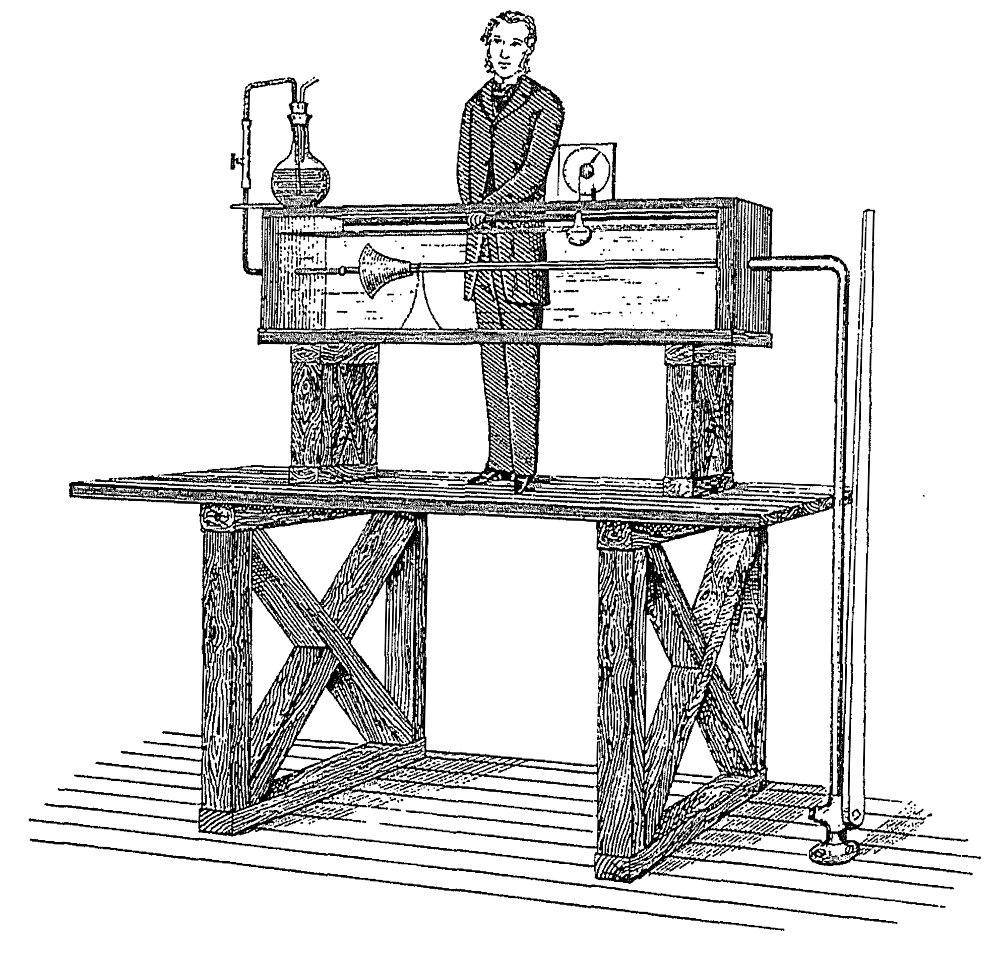
\includegraphics[width=\linewidth]{external/rayleigh_tubulence.jpg}
\end{image}%
\tcblower
\end{figureptx}%
%
\par
The description of this unit in the \href{http://www.bath.ac.uk/catalogues/2025-2026/ma/MA32051.html}{official catalogue} is the following:%
\begin{descriptionlist}
\begin{dlinarrow}{Aims}{frontmatter-3-3-2-1}%
In this unit you will explore the mathematical theory of fluid dynamics, with a view towards applications to physical phenomena such as flight, vortex motion and water waves. You will study the mathematics of conservation laws and the derivation of governing fluid dynamical equations. This unit will provide you with a foundation for further study of more advanced theory of fluid dynamics and continuum mechanics, and its application in scientific areas including engineering, physics and biology.%
\end{dlinarrow}%
\begin{dlinarrow}{Outcomes}{frontmatter-3-3-2-2}%
(i) Demonstrate an understanding of the principles of mathematical fluid dynamics; (ii) discuss and apply techniques from vector calculus and complex variable theory to analyse and solve fluid flow problems; (iii)  give a qualitative and quantitative account of a range of phenomena in fluid dynamics.%
\end{dlinarrow}%
\begin{dlinarrow}{Content}{frontmatter-3-3-2-3}%
Complex analysis primer: Cauchy-Riemann equations; harmonic functions; complex maps; residue integration. The mathematics of fluid phenomena and its applications: derivation and interpretation of governing equations; reduction of governing equations to equations of simpler formulation; potential flow; vortical flow. Two-dimensional incompressible and irrotational flow: velocity potential; stream function; complex potential. Conformal mapping. Vortex motion: vortex lines and tubes; Kelvin circulation theorem; Helmholtz' principal. Water waves: free surfaces; harmonic waves; finite depth; instability; group velocity. Computational fluid dynamics.%
\end{dlinarrow}%
\end{descriptionlist}
%
\end{preface}
%
%
\typeout{************************************************}
\typeout{Preface  History of the unit}
\typeout{************************************************}
%
\begin{preface}{Preface}{History of the unit}{}{History of the unit}{}{}{history}
Previously at Bath in the Mathematical Sciences, there were two units meant to teach continuum and fluid mechanics (or dynamics) to students. Prior to 2025, there was the \href{https://www.bath.ac.uk/catalogues/2024-2025/ma/MA30253.html}{MA30253 Continuum Mechanics} module. This was then continued into the \href{https://www.bath.ac.uk/catalogues/2024-2025/ma/MA40255.html}{MA40255 Viscous fluid dynamics} module.%
\par
As part of the curriculum transformation (with the first change to Year 3 in 2025), we are attempting to unify these two treatments, providing a more streamlined teaching of elementary fluid dynamics, which is oriented towards a broad range of styles of emphasis, from applied mathematics, to physics and engineering. The hope is that this new course on Fluid Dynamics provides you with a strong foundation in different basic fluid flows and their mathematical formulation and study.%
\end{preface}
%
%
\typeout{************************************************}
\typeout{Preface  Related units at Bath}
\typeout{************************************************}
%
\begin{preface}{Preface}{Related units at Bath}{}{Related units at Bath}{}{}{frontmatter-5}
We will only mention units from Year 2 onwards in this. Apart from the key pre-requisites of MA22016 (Differential equations and vector calculus) and\slash{}or MA20223 (the older Vector calculus and partial differential equations), we make an effort to keep the material in the module self-contained. You are recommended to have taken MA22021 (partial differential equations).%
\par
%
\begin{itemize}[label=\textbullet]
\item{}\lititle{MA22016: Differential equations and vector calculus.}\par%
\href{https://www.bath.ac.uk/catalogues/2024-2025/ma/MA22016.html}{This unit} forms a standard second-year module on differential equations and vector calculus, and is a key pre-requisite for this module. In addition to teaching and reviewing basic techniques for solving ordinary differential equations, you will learn about some of the core methods in vector calculus (directional derivatives; gradients; potentials; line integrals; divergence; curl; surface and volume integrals; curvilinear coordinates; integral theorems).%
\par
Note prior to curriculum transformation, this would have been part of the MA20223 unit (with additional material from the below MA22021).%
\item{}\lititle{MA22021: Partial differential equations.}\par%
\href{https://www.bath.ac.uk/catalogues/2024-2025/ma/MA22021.html}{This module} teaches basic techniques and theory for the core PDEs (Laplace, heat, wave equations). Generally, we will make with your broad familiarity of PDE different equation types and terminology (e.g. boundary conditions). This unit will be useful, as it will teach you some basic familiarity with partial differential equations. However, the current fluid dynamics module assumes you may not have taken it, and attempts to fill in any necessary gaps.%
\item{}\lititle{MA32045: Complex analysis.}\par%
\href{https://www.bath.ac.uk/catalogues/2025-2026/ma/MA32045.html}{This module} covers some of the theory and applications behind complex-valued functions. You will have encountered complex functions, e.g. \(f(z) = z^2, \e^z, \log z, \ldots\) in an \emph{ad-hoc} way, perhaps in earlier courses on Analysis. Again, we will attempt to cover all the necessary pre-requisites, and also provide you with helpful references.%
\end{itemize}
%
\end{preface}
%
%
\typeout{************************************************}
\typeout{Preface  Moodle and other references}
\typeout{************************************************}
%
\begin{preface}{Preface}{Moodle and other references}{}{Moodle and other references}{}{}{frontmatter-6}
Besides this document, the main resource for this unit is the \href{https://moodle.bath.ac.uk/course/view.php?id=62758}{Moodle page}. Links to the video recordings, course notes, and other resources are collected there.%
\par
There are countless fluid mechanics or fluid dynamics courses and textbooks, and for the most part, the development of a \emph{first course} on fluid dynamics tends to be quite similar between universities and treatments. If you would like additional references, here are a few useful ones.%
\par
However, note that our goal is to be as self-sufficient as possible via the lecture notes.%
\par
%
\begin{itemize}[label=\textbullet]
\item{}David Acheson's (1990) book \emph{Elementary fluid dynamics} \hyperlink{ref-acheson}{[{\xreffont 4}]}: a significant part of this course follows some of the now-classic treatments that would have been developed simultaneous to the design of this book by Acheson (often used by Oxford UG students). It is written in quite an informal style.%
\par
\begin{image}{0.35}{0.3}{0.35}{}%
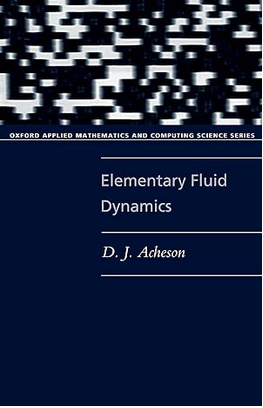
\includegraphics[width=\linewidth]{external/intro_book_acheson.png}
\end{image}%
%
\item{}Multimedia Fluid Mechanics Online, edited by G. M. Homsy \hyperlink{ref-homsy}{[{\xreffont 1}]}: a collection of videos and explanations of various fluid mechanics phenomena. This is an online resource available through the University of Bath library system.%
\par
\begin{image}{0.35}{0.3}{0.35}{}%

\includegraphics[width=\linewidth]{external/ch-frontmatter-9781108583756.jpg}
\end{image}%
%
\item{}Milton Van Dyke's (1982) book "An album of fluid motion" \hyperlink{ref-album}{[{\xreffont 3}]}: a classic album showing beautiful black and white images of fluid motion. Published by an iconic private press and sold (by design by Van Dyke) at affordable prices!%
\par
\begin{image}{0.35}{0.3}{0.35}{}%
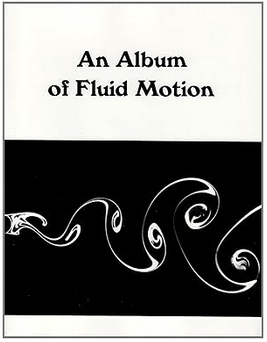
\includegraphics[width=\linewidth]{external/intro_book_vandyke.png}
\end{image}%
%
\item{}Kreyszig, E. (2007) book "Advanced engineering mathematics" \hyperlink{ref-kreyszig}{[{\xreffont 2}]} covers all the necessary essentials in terms of Vector Calculus and Complex Variables. This is one of my favourite reference texts for mathematical methods just on account of how straightfoward it is. Despite the "engineering" in the title, the style of presentation here fits in well with the style of UK applied mathematics.%
\par
\begin{image}{0.35}{0.3}{0.35}{}%
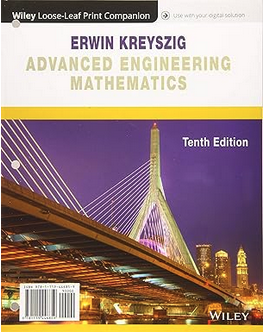
\includegraphics[width=\linewidth]{external/intro_book_eng.png}
\end{image}%
%
\end{itemize}
%
\end{preface}
%% begin: table of contents
%% Adjust Table of Contents
\setcounter{tocdepth}{1}
\renewcommand*\contentsname{Contents}
\tableofcontents
%% end:   table of contents
\mainmatter
%
%
\typeout{************************************************}
\typeout{Chapter 1 Introduction}
\typeout{************************************************}
%
\begin{chapterptx}{Chapter}{Introduction}{}{Introduction}{}{}{ch-chapter01-introduction}
\renewcommand*{\chaptername}{Chapter}
\begin{introduction}{}%
\begin{quote}%
Now I think hydrodynamics is to be the root of all physical science, and is at present second to none in the beauty of its mathematics.%
\nopagebreak\par%
\hfill\textemdash{}{\setlength{\tabcolsep}{0pt}\begin{tabular}[t]{l@{}}
William Thompson (Lord Kelvin), Dec. 1857.
\end{tabular}}\\\par
\end{quote}
As evidenced by the quotation above, during the great Victorian era, Lord Kelvin had predicted that the field of hydronamics (predominantly, the study of liquids) would reign over all the physical sciences. Today that is not quite true, in the sense that hydrodynamics is only one of many sub-branches of the wider study of fluid motion. However, Kelvin's prediction is certainly true in spirit: there are very few branches in the physical sciences, from biology and chemistry, to engineering and physics, where the study of fluid mechanics does not possess strong historical and scientific connections. The principles, language, and techniques of fluid mechanics begin from the fundamental laws of conservation; in their form, one can argue that all of nature can be derived-{}-{}-this grandiose point is, to some extent, what Kelvin had meant when he referred to being the "root of all physical science".%
\par
Moreover, countless areas of mathematics, from the 19th century and onwards, have been developed as a direct consequence of the need to investigate the beautiful nature of fluid motion. These include everything from the theory of ordinary and partial differential equations, calculus, complex analysis, mathematical methods and approximation theory, geometry and topology, analysis, numerical methods and numerical analysis, industrial and applied mathematics, and so forth and so on.%
\begin{remark}{Remark}{Fluid mechanics vs. fluid dynamics.}{ch-chapter01-introduction-2-4}%
Why is this course called fluid dynamics and yet fluid mechanics? What is the difference?%
\par
In general, fluid mechanics includes both "statics" (fluids at rest) and "dynamics" (things in motion). This is a distinction that, in the authors' opinions, mathematicians rarely use (we probably refer to "fluid mechanics" more commonly so as to avoid being specific); these distinctions are perhaps more important in engineering. For example, the study of the shape of a soap film or bubble between a wire hoop is a question of statics; but the behaviour of the soap or bubble if it moves or pops is a question of dynamics!%
\par
A tree diagram of different subfields and their applications might be made as follows.%
\begin{preformatted}
Fluid Mechanics
 ├── Fluid Statics
 │     ├── Hydrostatics → Pressure in tanks and dams
 │     ├── Buoyancy → Ship and submarine design
 │     └── Manometry → Pressure measurement in pipelines
 │
 └── Fluid Dynamics
       ├── Inviscid Flow
       │     ├── Potential Flow → Aerodynamics of airfoils
       │     └── Compressible Flow (ideal gases) → Supersonic jet nozzles
       │
       ├── Viscous Flow
       │     ├── Internal Flows (pipe/duct flow) → Water distribution networks
       │     ├── External Flows (boundary layers) → Drag on cars and airplanes
       │     └── Lubrication Theory → Bearings in machines
       │
       ├── Turbulence
       │     ├── Atmospheric Turbulence → Weather prediction
       │     └── Industrial Turbulence → Mixing in chemical reactors
       │
       └── Multiphase Flow
             ├── Gas–Liquid Flow → Oil & gas pipelines
             ├── Liquid–Solid Flow → Slurry transport in mining
             └── Gas–Solid Flow → Fluidized bed reactors
\end{preformatted}
It is not uncommon for some scientists and mathematicians to devote their entire careers to an entire subbranch of fluid mechanics. Some university departments will focus solely on certain subbranches as well! Hence fluid mechanics is for many, a lifelong pursuit!%
\end{remark}
What is the course about?%
\par
Our first task, starting in \hyperref[ch-chapter02-kinematics]{Chapter~{\xreffont\ref{ch-chapter02-kinematics}}} and \hyperref[ch-chapter03-equations]{Chapter~{\xreffont\ref{ch-chapter03-equations}}} is to derive the so-called Euler equation, given by%
\begin{equation*}
\rho\left(\pd{\bu}{t} + (\bu \cdot \nabla)\bu\right) = -\nabla p + \rho\bg.
\end{equation*}
Euler's equation relates the velocity of a fluid, \(\bu\), with its density \(\rho\), pressure \(p\), and associated forces, \(\bg\). It is an expression of the conservation of momentum of fluid, and is completed with an accompanying equation for conservation of mass. Together, the two equations are solved with the specification of additional boundary conditions to describe many liquids, from the water in your bathtub, to the water in the ocean as a ship travels through the surface.%
\par
Slowly, we will begin to appreciate the use of conservation laws, and the mathematics necessary, to derive the above equations (compressing some hundred years of scientific work into only a handful of lectures!). We will also appreciate that, despite their compact form, the above equations are certainly not easy to solve!%
\begin{figureptx}{Figure}{Flow around an airfoil is an example of potential flow theory. From Van Dyke, An Album of Fluid Motion.}{ch-chapter01-introduction-2-8}{}%
\begin{image}{0}{1}{0}{}%
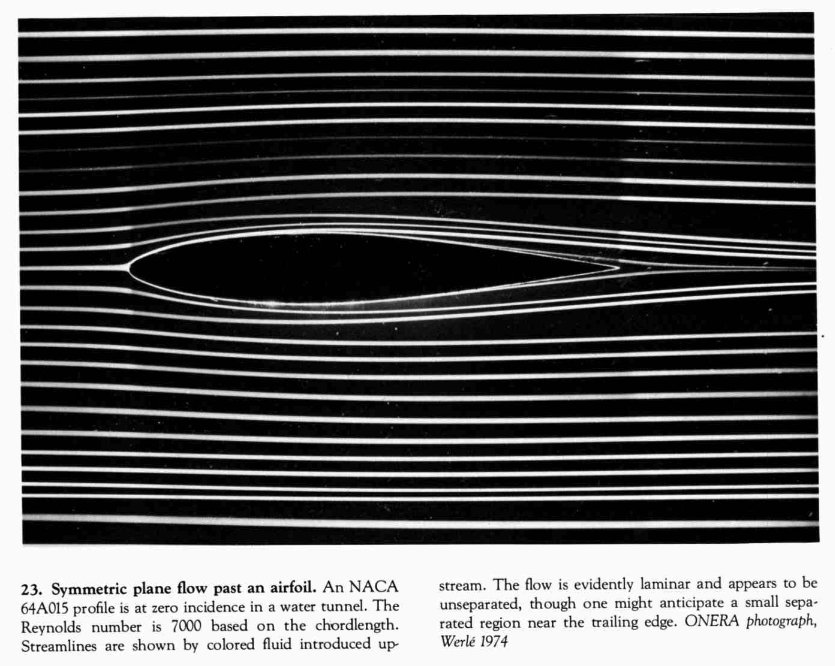
\includegraphics[width=\linewidth]{external/airfoil.png}
\end{image}%
\tcblower
\end{figureptx}%
Our next task, starting in \hyperref[ch-chapter04-potentialflows]{Chapter~{\xreffont\ref{ch-chapter04-potentialflows}}} is to study a particular simplification of the Euler equation that yields the flow of an \emph{ideal} or \emph{potential} fluid. Under such constraints, instead of solving the above difficult equations, we solve a much simpler equation:%
\begin{equation*}
\nabla^2 \phi = 0,
\end{equation*}
for a so-called \emph{velocity potential}, \(\phi\), related to the velocity by \(\bu = \nabla \phi\). Potential flow theory would have occupied some of the greatest minds of our time, from Euler, Lagrange, Bernoulli, d'Alembert, and Laplace of the 18th century; to the great Victorian scientists of the 19th century: Kelvin, Green, Stokes, Helmholtz; then towards the modern 20th century workers such as Prandtl, Lighthill, Milne-Thompson, and so forth. It is the simplest framework for studying the motion of a liquid, such as water, but enjoys incredibly deep connections with the beautiful theory of complex variables. We will study some of these connections, leading to learning about things such as conformal mapping theory.%
\begin{figureptx}{Figure}{In 1887, Kelvin famously predicted that the waves trailing a ship produce a wedge of approximately \(2 \times 19.5^\circ\). This theory belongs to the analysis of linear water waves (though it is unlikely we will have time to reproduce Kelvin's approximation!) From Van Dyke, An Album of Fluid Motion.}{ch-chapter01-introduction-2-10}{}%
\begin{image}{0.15}{0.7}{0.15}{}%
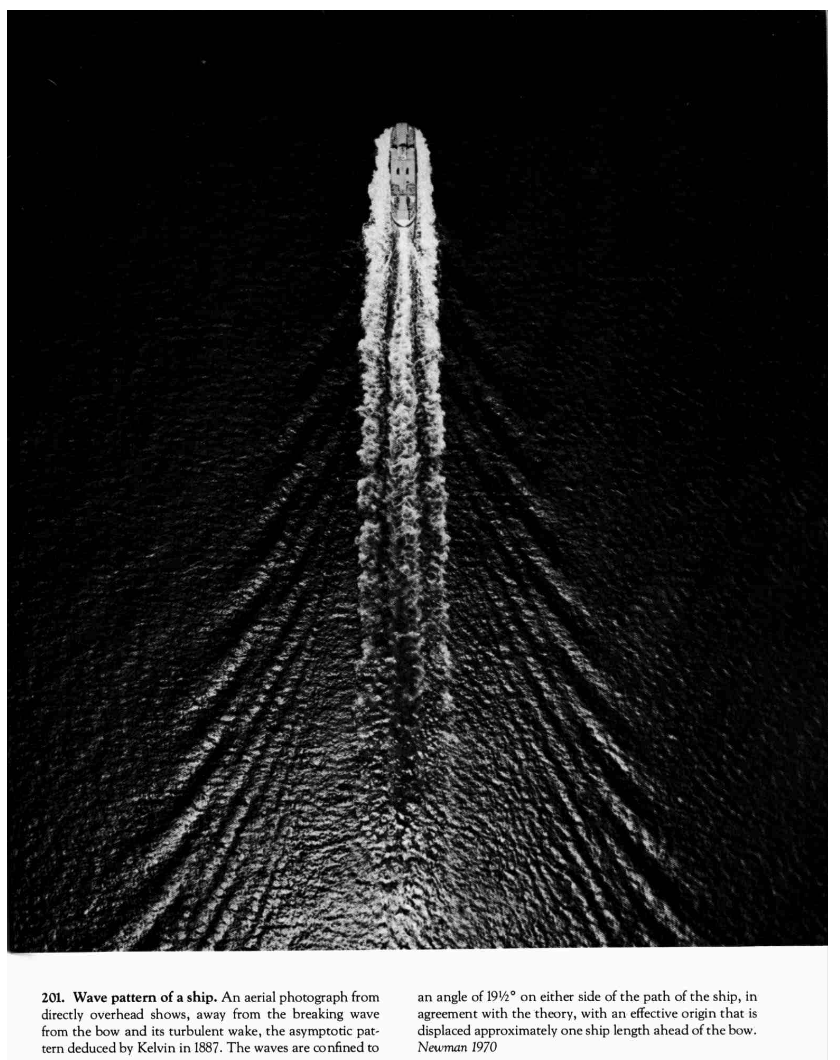
\includegraphics[width=\linewidth]{external/kelvinwave.png}
\end{image}%
\tcblower
\end{figureptx}%
Water waves is probably the application that was at the forefront of Lord Kelvin's thoughts when he discussed the state of hydrodynamics in the quotation that begins in \hyperref[ch-chapter05-waves]{Chapter~{\xreffont\ref{ch-chapter05-waves}}}. The study of the surface motion of water introduces a seemingly minor complexity that is responsible for great heartache: the fluid is now bounded by an unknown free surface, which much now be solved as part of the problem! The theory of water waves was at the heart of many minds in the 19th century, given its importance in all applications naval and oceanic. The study of water waves begins with so-called linear wave theory, and moves towards numerical solutions of the full Euler equations.%
\begin{figureptx}{Figure}{Water ejected from a nozzle forms a vortex sheet that rolls up into two vortex rings. From Van Dyke (1982) "An Album of Fluid Motion" \hyperlink{ref-album}{[{\xreffont 3}]}.}{ch-chapter01-introduction-2-12}{}%
\begin{image}{0.15}{0.7}{0.15}{}%
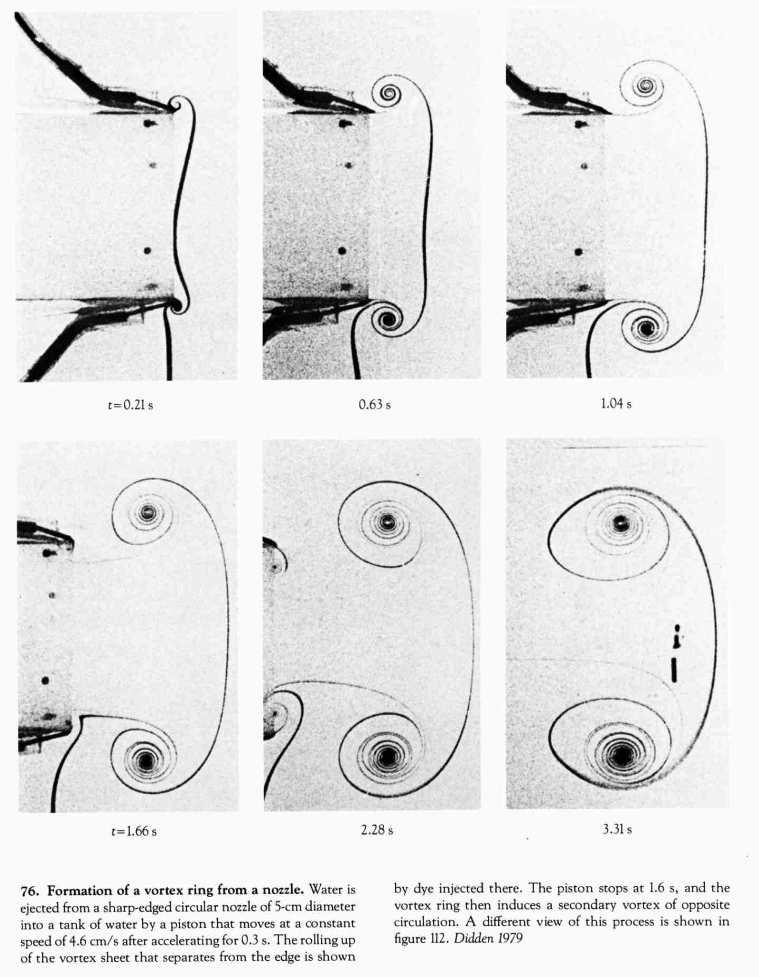
\includegraphics[width=\linewidth]{external/vortexring.png}
\end{image}%
\tcblower
\end{figureptx}%
In the above applications, our attention will be focused on so-called irrotational flows: flows that either do not contain or do not introduce new rotational characteristics. Of course, real life fluids are rarely so well-behaved and indeed, the study of vortices is an important domain in its own right, leading to models for tornados, flight, and many other fluid phenomena. The principle character of \hyperref[ch-chapter06-vorticity]{Chapter~{\xreffont\ref{ch-chapter06-vorticity}}} is the vorticity, \(\omega = \nabla \times \bu\). What is vorticity, how does one measure it, and what is its role in governing fluid motion: these are the topics of this chapter.%
\begin{figureptx}{Figure}{As illustrated in \hyperref[fig-rayleigh]{Figure~{\xreffont\ref{fig-rayleigh}}}, in 1883 Rayleigh performed a famous experiment of stability of flow in a tube, showing the emergence of an instability as the speed of the flow is increased. This leads to turbulence, which is predicted, in principle, from the Navier-Stokes equations of viscous flows. (From Van Dyke, An Album of Fluid Motion.}{ch-chapter01-introduction-2-14}{}%
\begin{image}{0.15}{0.7}{0.15}{}%
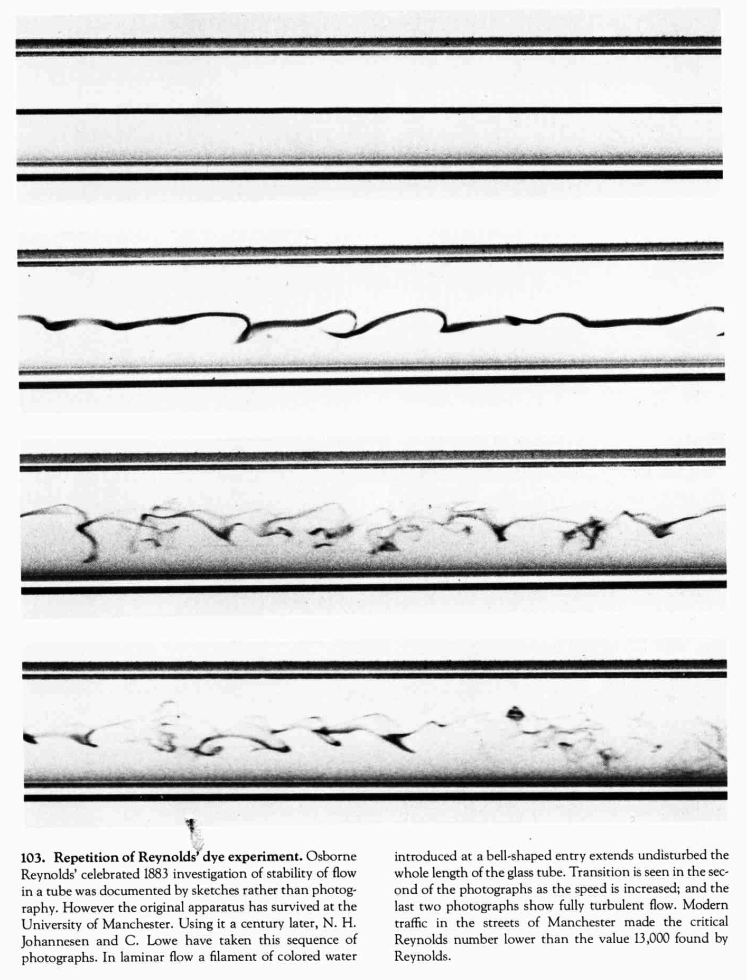
\includegraphics[width=\linewidth]{external/turbulence.png}
\end{image}%
\tcblower
\end{figureptx}%
Finally, the last part of this course will open up to the important discpline of viscous flows in \hyperref[ch-viscousflows]{Chapter~{\xreffont\ref{ch-viscousflows}}}. For this, the Euler equations are no longer sufficient, and we must include a dissipative component,%
\begin{equation*}
\rho\left(\pd{\bu}{t} + (\bu \cdot \nabla)\bu\right) = -\nabla p + \rho \bg + \mu \nabla^2 \bu,
\end{equation*}
with \(\mu\) being the \emph{viscosity} of the fluid. The above equation, together with an equation for conservation of mass, forms the so-called \emph{Navier-Stokes equations}. All fluids are viscous to some extent, though some moreso than others. You will learn about the connections between viscous flow theory and inviscid theory, and some of the simple viscous flows that are foundational in this subbranch.%
\end{introduction}%
%
%
\typeout{************************************************}
\typeout{Section 1.1 A reminder of vector calculus}
\typeout{************************************************}
%
\begin{sectionptx}{Section}{A reminder of vector calculus}{}{A reminder of vector calculus}{}{}{sec-preliminary-vector-calculus}
\begin{figureptx}{Figure}{George Green's monumental work on electricity and magnetism, making use of many new concepts in vector calculus, 1828.}{fig-intro-green}{}%
\begin{image}{0.25}{0.5}{0.25}{}%
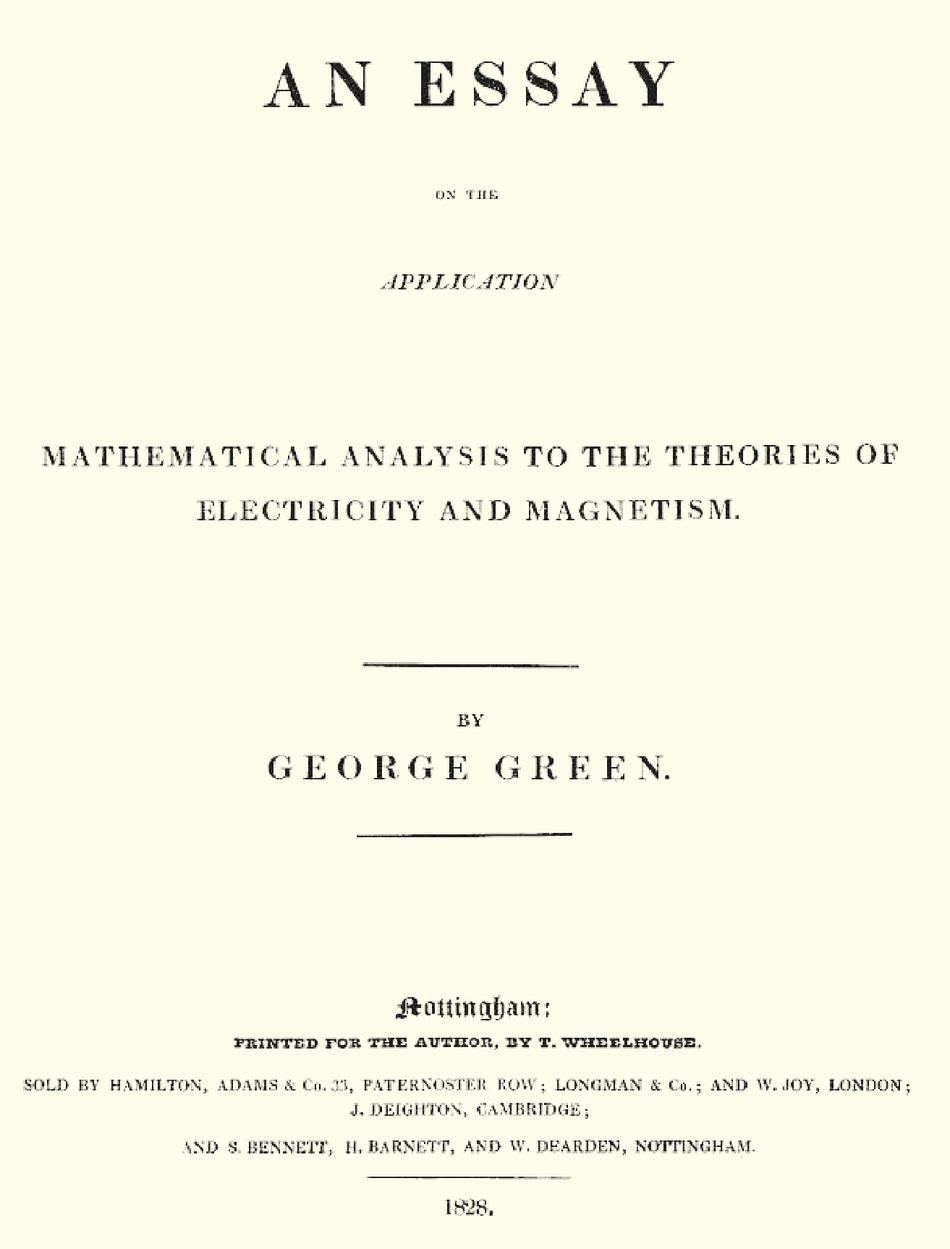
\includegraphics[width=\linewidth]{external/GreenEssay.png}
\end{image}%
\tcblower
\end{figureptx}%
During the first week, we will provide a very brief review of some of the necessities that you may require in terms of vector calculus. Many of you will have taken the MA20223 Vector Calculus and Partial Differential Equations module, and a version of the 2024-25 lecture notes has been updated for easy reference \href{https://moodle.bath.ac.uk/course/view.php?id=62758}{on Moodle}.%
\par
We will assume that you are familiar enough with how to interpret many of the vector calculus identities found in Sec. 10 of the University of Bath book of tables, which can be access on Moodle or \href{https://people.bath.ac.uk/ensdasr/ME10304.bho/UniBathFormulaeAndStatisticalTables.pdf}{via this link}.%
\par
In general, over the next few weeks, you will want to be familiar with recalling\slash{}looking up concepts like:%
\begin{itemize}[label=\textbullet]
\item{}The use of identities like div curl = 0 and curl grad = 0. Some of these are found on p.24 of the above tables.%
\item{}The notion of line integrals, surface integrals, and volume integrals.%
\item{}The divergence theorem and Stokes' theorem. (p.24)%
\item{}Conversion of vector operations and integrals into different coordinate systems (p.25)%
\end{itemize}
%
\end{sectionptx}
%
%
\typeout{************************************************}
\typeout{Section 1.2 A reminder of complex variables}
\typeout{************************************************}
%
\begin{sectionptx}{Section}{A reminder of complex variables}{}{A reminder of complex variables}{}{}{sec-preliminary-complex-variables}
\begin{introduction}{}%
In \hyperref[ch-chapter04-potentialflows]{Chapter~{\xreffont\ref{ch-chapter04-potentialflows}}}, we will leverage the power of complex variables to study certain problems in fluids (flow of a potential flow). One concept that you may be unfamiliar with at this stage is the concept of a \emph{branch cut}.%
\begin{figureptx}{Figure}{An image from Tristan Needham's "Visual Complex Analysis" \hyperlink{ref-needham}{[{\xreffont 5}]} showing how complex mappings transform shapes from one region to another.}{fig-intro-needham}{}%
\begin{image}{0.1}{0.8}{0.1}{}%
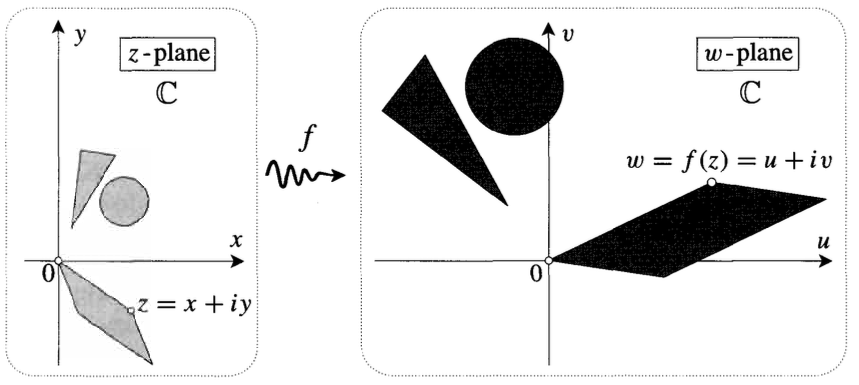
\includegraphics[width=\linewidth]{external/intro_needham.png}
\end{image}%
\tcblower
\end{figureptx}%
\end{introduction}%
%
%
\typeout{************************************************}
\typeout{Subsection 1.2.1 Basic complex representations}
\typeout{************************************************}
%
\begin{subsectionptx}{Subsection}{Basic complex representations}{}{Basic complex representations}{}{}{sec-preliminary-complex-variables-3}
Generally, we write the Cartesian and polar form of a complex number as,%
\begin{equation*}
z = x + \im y = r\e^{\im\theta},
\end{equation*}
for magnitude \(r > 0\) and angle \(\theta\). Below, we will consistently refer to \(z\in\mathbb{C}\). The decomposition of the complex exponential is given by Euler's identity:%
\begin{equation}
\e^{\im\theta} = \cos \theta + \im \sin\theta.\label{eq-complex-euler}
\end{equation}
%
\par
The usual trigonometric functions can be extended to the complex plane by considering their definition in terms of complex exponentials and Euler's identity. For example, we have%
\begin{equation}
\cos z = \frac{\e^{\im z} + \e^{-\im z}}{2} \quad \text{and} \quad \sin z = \frac{\e^{\im z} - \e^{-\im z}}{2\im}.\label{eq-complex-cossin}
\end{equation}
%
\par
Another important function we shall consider is the complex logarithm, defined as%
\begin{equation}
\log z \equiv \log r + \im \theta,\label{eqn-intro-complex-log}
\end{equation}
where \(z = r\e^{\im\theta}\). That this definition is sensible is verified by checking that the logarithm is the inverse of the exponential. That is,%
\begin{equation*}
\e^{\log z} = \e^{\log r + \im\theta} = \e^{\log r} \e^{\im\theta} = z.
\end{equation*}
%
\par
However, the definition \hyperref[eqn-intro-complex-log]{({\xreffont\ref{eqn-intro-complex-log}})} is troubling because it is not single-valued. For example, writing \(z = 1 \e^{\im \cdot 0}\) and \(z = 1 \e^{\im \cdot 2\pi}\) gives two different possible values of \(\log z\) for the same value of \(z = 1\). We dig deeper into this issue.%
\end{subsectionptx}
%
%
\typeout{************************************************}
\typeout{Subsection 1.2.2 Complex functions}
\typeout{************************************************}
%
\begin{subsectionptx}{Subsection}{Complex functions}{}{Complex functions}{}{}{sec-preliminary-complex-variables-4}
A complex function maps points on the complex plane to points on the complex plane. For instance, the square function,%
\begin{equation*}
f(z) = z^2 = r^2 \e^{2\im \theta},
\end{equation*}
can be better understood by its effect on points on the unit circle, \(|z| = 1\).%
\par
Consider a particle that orbits around the unit circle in the \(z-\)plane at unit speed. If the particle rotates by half a revolution, with \(\theta = \pi\), then in the image plane, the image particle has rotated by a full revolution, with \(f(z) = (\e^{\im \pi})^2\) in this same unit time. This is illustrated by the image in \hyperref[fig-intro-z2map]{Figure~{\xreffont\ref{fig-intro-z2map}}}.%
\begin{figureptx}{Figure}{A revolution of \(\pi\) in the pre-image produces a full rotation in the image plane.}{fig-intro-z2map}{}%
\begin{image}{0}{1}{0}{}%
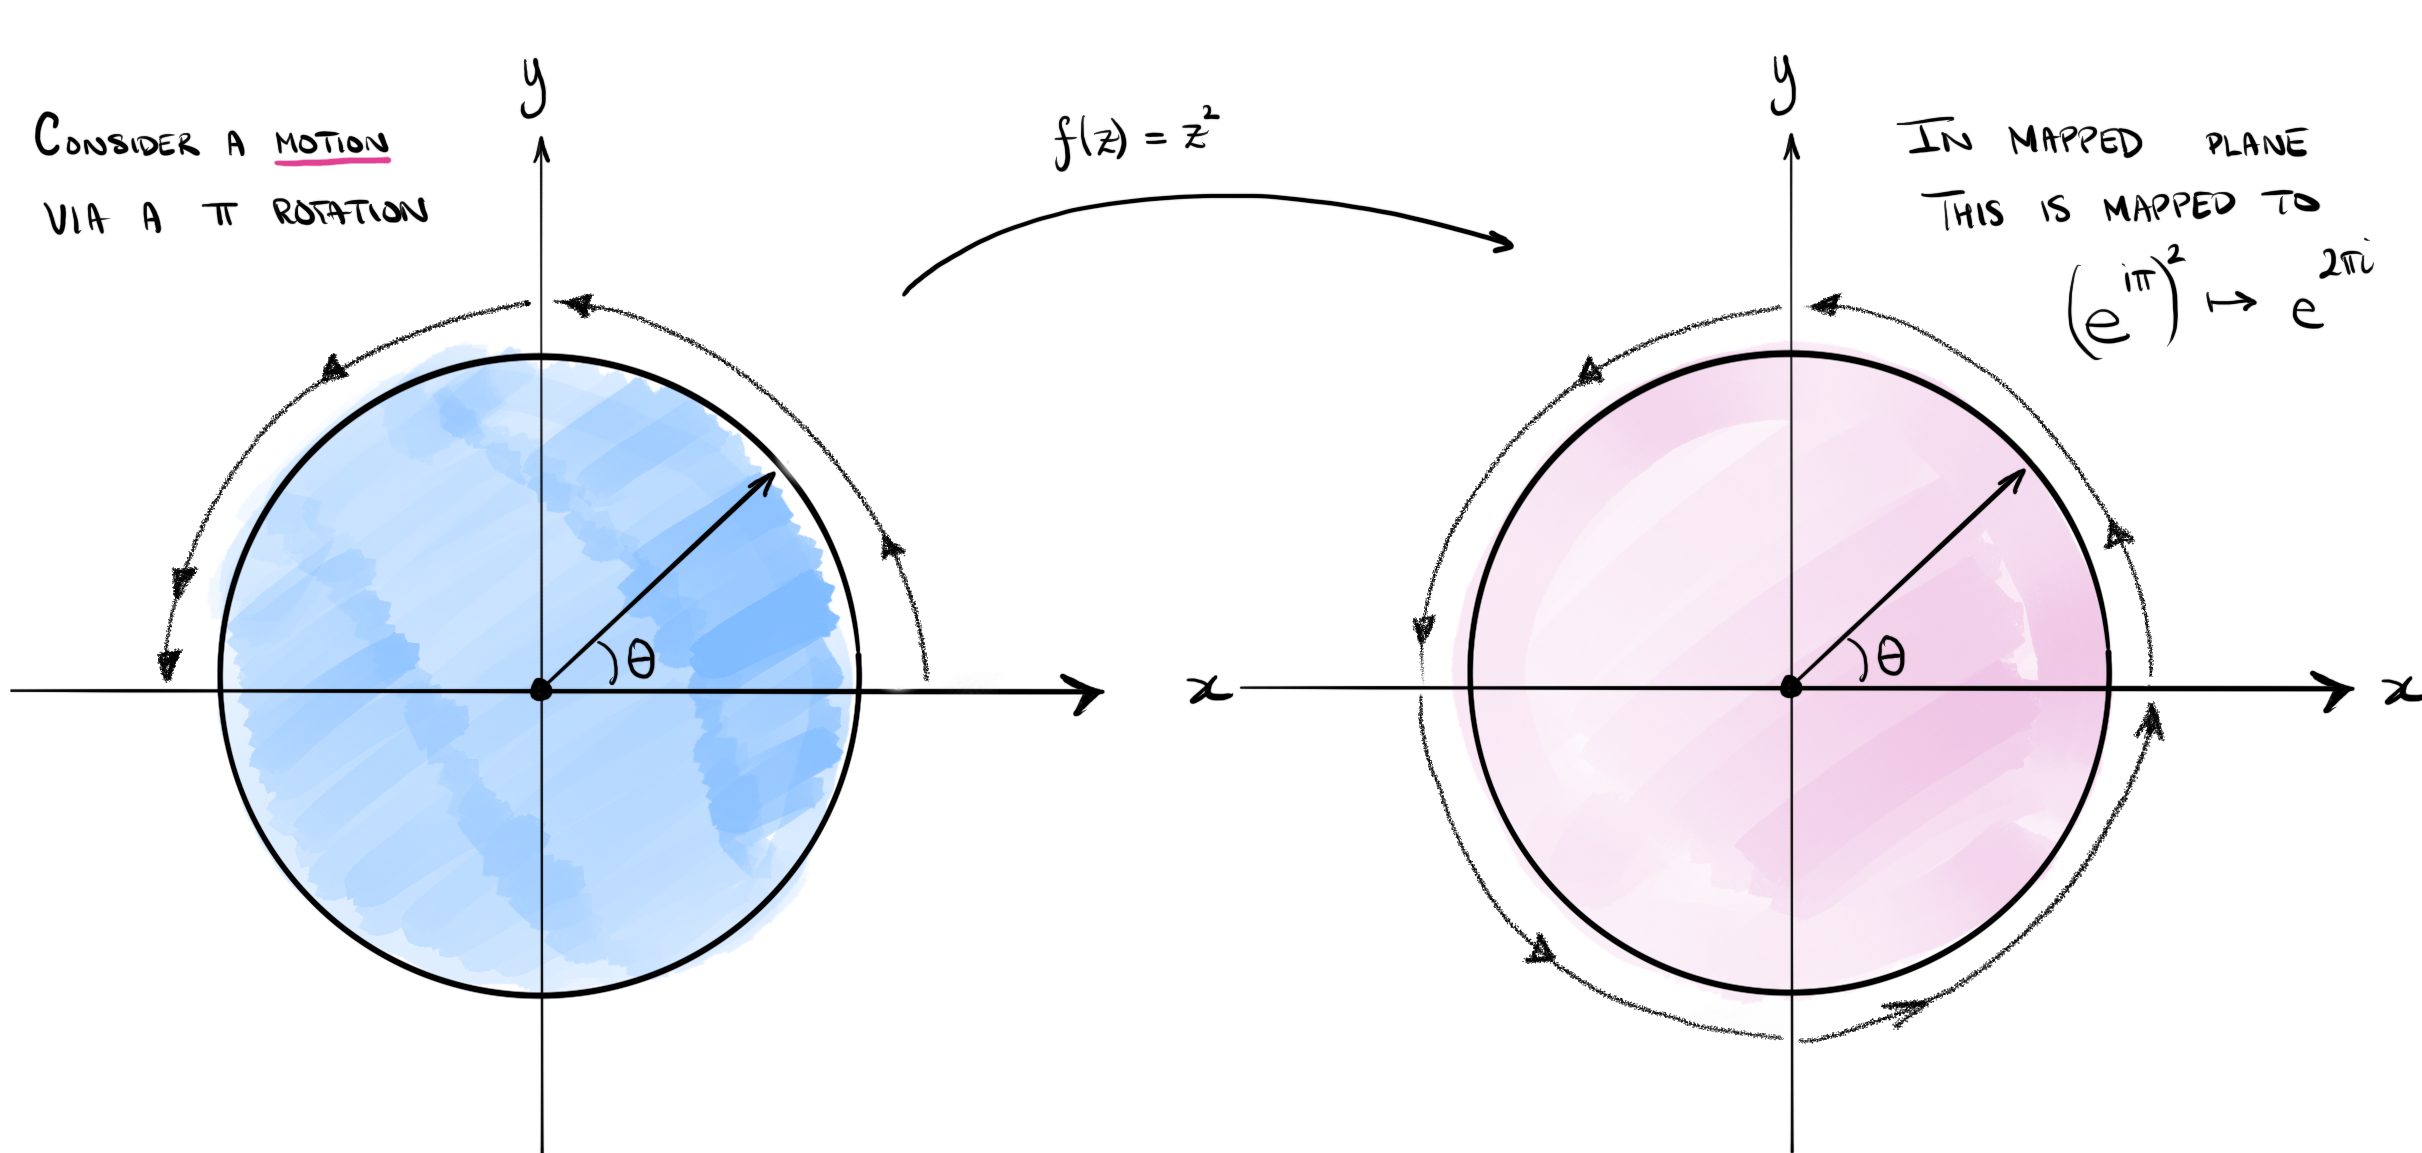
\includegraphics[width=\linewidth]{external/intro_z2map.png}
\end{image}%
\tcblower
\end{figureptx}%
Now we continue rotating around the unit circle in the \(z-\)plane, performing an additional \(\pi\) rotation. Within the image plane, the particle has now completed another full rotation around the unit circle. This is shown in \hyperref[fig-intro-z2map_02]{Figure~{\xreffont\ref{fig-intro-z2map_02}}}.%
\begin{figureptx}{Figure}{A revolution of \(\pi\) in the pre-image produces a full rotation in the image plane.}{fig-intro-z2map_02}{}%
\begin{image}{0}{1}{0}{}%
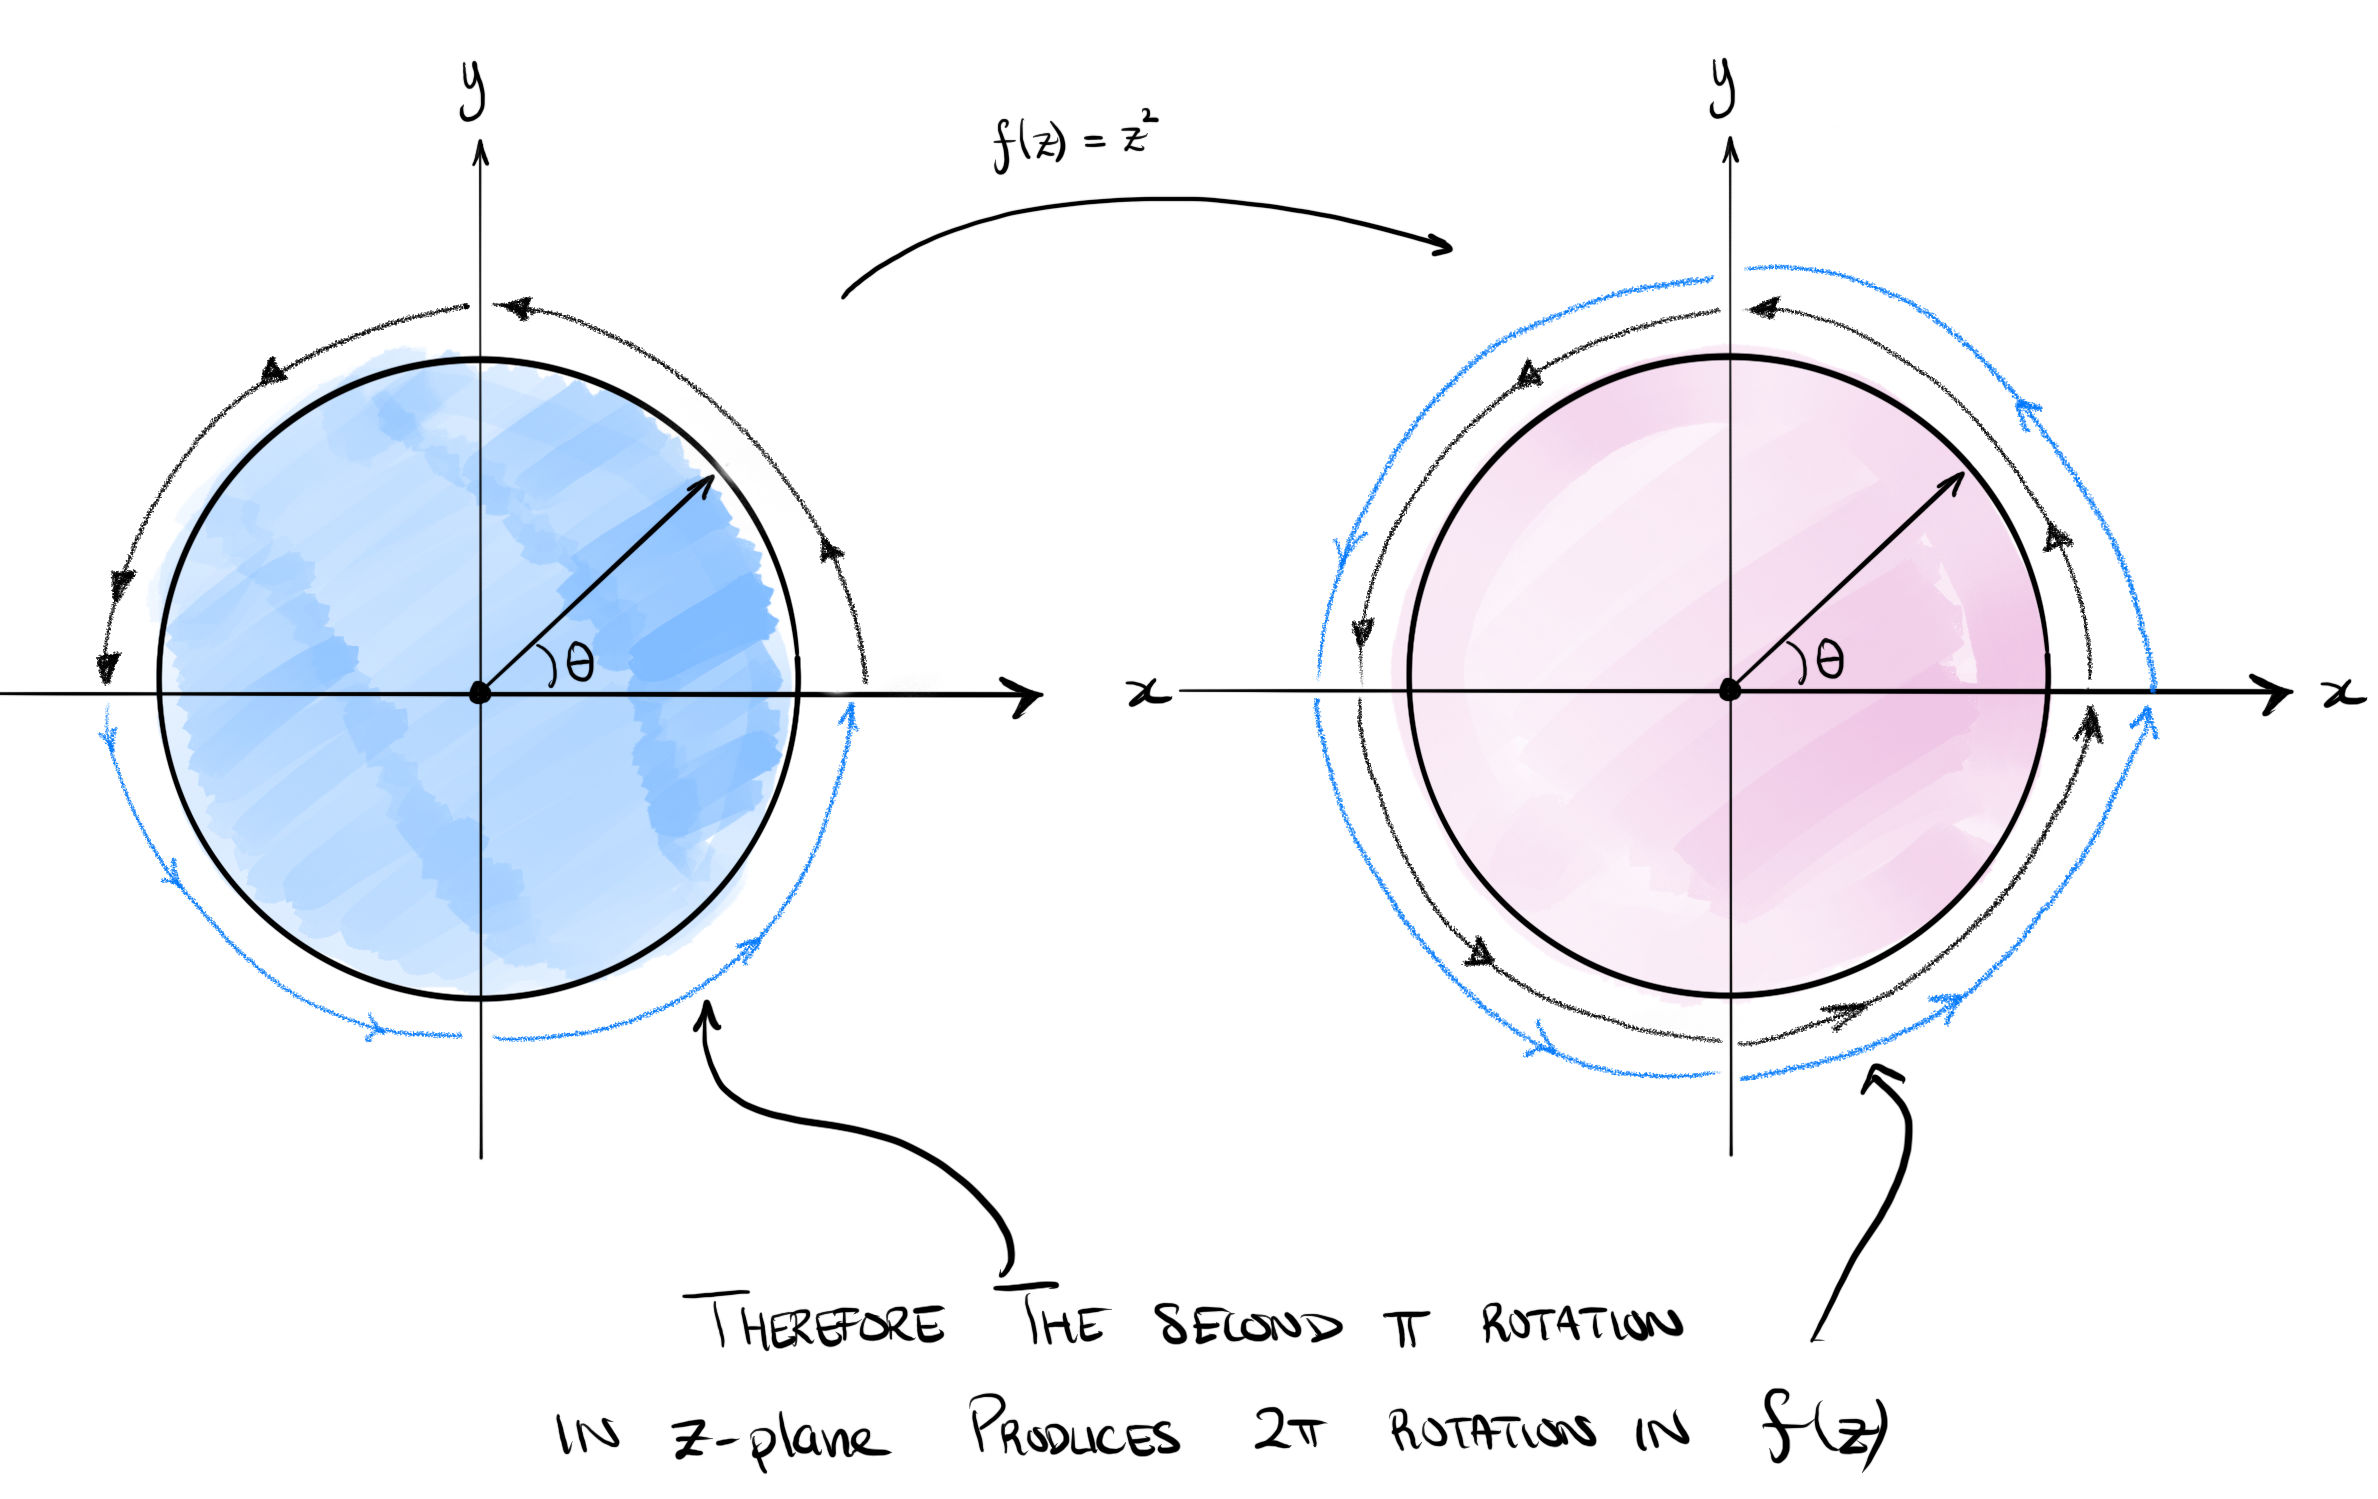
\includegraphics[width=\linewidth]{external/intro_z2map_02.jpg}
\end{image}%
\tcblower
\end{figureptx}%
\end{subsectionptx}
%
%
\typeout{************************************************}
\typeout{Subsection 1.2.3 Multifunctions, branch cuts, and Riemann sheets}
\typeout{************************************************}
%
\begin{subsectionptx}{Subsection}{Multifunctions, branch cuts, and Riemann sheets}{}{Multifunctions, branch cuts, and Riemann sheets}{}{}{sec-preliminary-complex-variables-5}
Now consider the inverse function of the above, given by the square root function,%
\begin{equation*}
f(z) = z^{1/2}.
\end{equation*}
%
\par
Visually, we can simply consider the same figures as before, but now with the mapping proceeding from the right subfigure to the left subfigure. Observe that there is now an ambiguity, because for each point in the original \(z-\)plane, there are two possible images to assign for \(z^{1/2}\), corresponding to either the top semicircle of the left figure, or the bottom semicircle.%
\par
That is, it is unclear of whether we should define:%
\begin{equation*}
f(z) = z^{1/2} = r^{1/2} \e^{\im\theta/2},
\end{equation*}
or%
\begin{equation*}
f(z) = z^{1/2} = -r^{1/2} \e^{\im\theta/2}.
\end{equation*}
%
\par
Moreover there is a problem, for if we allow a "motion" of the \(z\) values such that \(z\) rotates more than a complete revolution around the origin, then \(f(z)\) is no longer well-defined and takes on multiple possible values.%
\par
This leads to the following restriction. We define a \emph{branch cut} of the \(z-\)plane, and restrict the possible argument values. For example, we may choose%
\begin{equation*}
0 \leq \theta < 2\pi,
\end{equation*}
hence imposing that the branch cut is along the positive real axis. This is illustrated in \hyperref[fig-intro-branchcut]{Figure~{\xreffont\ref{fig-intro-branchcut}}} where the branch cut is shown as a wavy line.%
\begin{figureptx}{Figure}{Branch cut}{fig-intro-branchcut}{}%
\begin{image}{0.1}{0.8}{0.1}{}%
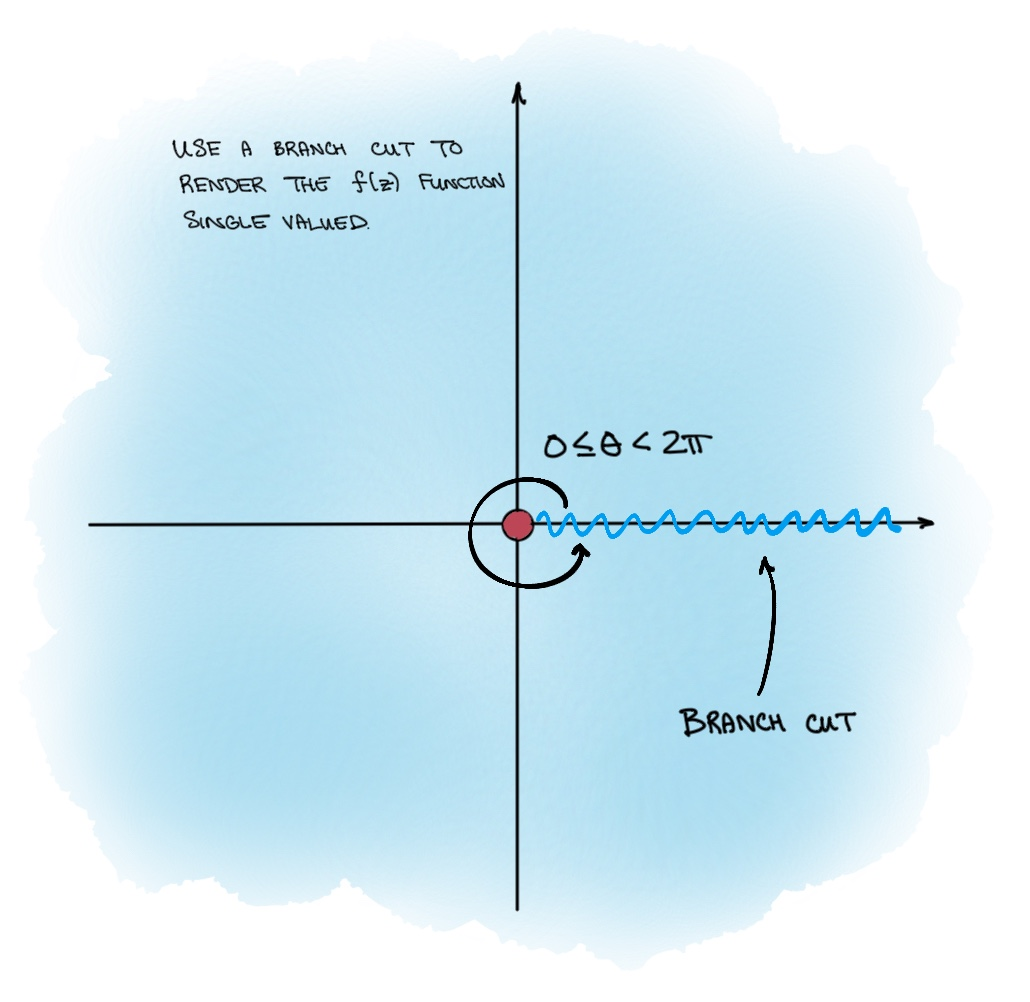
\includegraphics[width=\linewidth]{external/intro_branchcut.jpg}
\end{image}%
\tcblower
\end{figureptx}%
Alternatively, we could have equally chosen%
\begin{equation*}
-\pi \leq \theta < \pi,
\end{equation*}
hence taken the branch cut along the negative real axis.%
\par
Once the branch cut has been selected, the previous multi-function is restricted to one of the two possible definitions above. This leads to the definition as follows.%
\begin{definition}{Definition}{Branches of the square root function.}{sec-preliminary-complex-variables-5-10}%
The positive branch of the square root, with branch cut taken along the positive real axis, is defined by%
\begin{equation*}
f(z) = f_1(z) = z^{1/2} = r^{1/2} \e^{\im\theta/2},
\end{equation*}
for \(r > 0 \) and \(0 \leq \theta < 2\pi\). Other branch cut choices can be taken in an analogous manner (curve that extends from \(z= 0\) to \(z = \infty\)).%
\par
Then the above \(f\) with \(z\) restricted as given is a well-defined single-valued function.%
\par
There is an analogous negative branch defined as%
\begin{equation*}
f(z) = f_2(z) = z^{1/2} = -r^{1/2} \e^{\im\theta/2},
\end{equation*}
%
\par
Therefore, \(f_1\) and \(f_2\) make up the two "layers" of the square root function.%
\par
We often refer to each individual "layer" as a \emph{Riemann sheet}\index{Riemann sheet}. The critical point \(z = 0\) is referred to as a \emph{branch point}\index{branch point}.%
\par
The collection of Riemann sheets is referred to as a \emph{Riemann surface}\index{Riemann surface}.%
\end{definition}
In \hyperlink{ex-Riemannsurface}{Exercise~{\xreffont 1.3.1}}, you will plot the Riemann surface that corresponds to \(f(z) = z^{1/2}\). The result might look like this version created using Python graphing tool: \begin{figureptx}{Figure}{Riemann surface for the square root function. This shows the real part of the square root, which consists of both a positive branch and a negative branch. In the above case, we have placed the branch cut along the negative real axis.}{fig-intro-sqrt-surface}{}%
\begin{image}{0}{1}{0}{}%
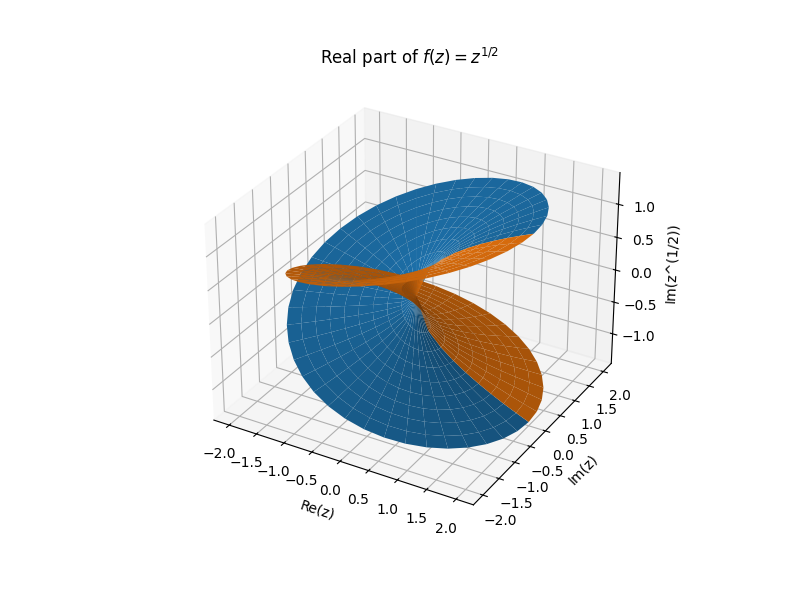
\includegraphics[width=\linewidth]{external/intro_sqrt_01.png}
\end{image}%
\tcblower
\end{figureptx}%
%
\par
A similar argument would indicate that the function%
\begin{equation}
f(z) = (z + 1)^{1/2} (z - 1)^{1/2},\label{eq-intro-twobranch}
\end{equation}
requires two branch cuts in general, each cut originating from the two branch points at \(z = \pm 1.\) You will study this function in more detail in \hyperlink{ex-branch1}{Exercise~{\xreffont 1.3.2}}.%
\par
Also in \hyperlink{ex-log}{Exercise~{\xreffont 1.3.3}}, you will study the branch structure of the complex logarithm in \hyperref[eqn-intro-complex-log]{({\xreffont\ref{eqn-intro-complex-log}})}.%
\end{subsectionptx}
%
%
\typeout{************************************************}
\typeout{Subsection 1.2.4 Other functions and visualisations}
\typeout{************************************************}
%
\begin{subsectionptx}{Subsection}{Other functions and visualisations}{}{Other functions and visualisations}{}{}{sec-preliminary-complex-variables-6}
The theory of complex analysis is rich in different kinds of visualisations. Another way to visualise a complex function is by considering its effect on a gridded pattern in the original \(z\)-plane, and then to imagine the function as warping this pattern. With this interpretation, it will be seen clearly that the operation of \(f(z) = z^2\) essentially rotates and expands the \((x, y)\) plane. This is seen in the following video.%
\begin{sidebyside}{2}{0.075}{0.075}{0.17}%
\begin{sbspanel}{0.47}%
\noindent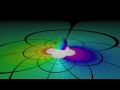
\includegraphics[width=\linewidth]{generated/youtube/sec-preliminary-complex-variables-6-3.jpg}
\end{sbspanel}%
\begin{sbspanel}{0.21}%
\noindent
\includegraphics[width=\linewidth]{generated/qrcode/sec-preliminary-complex-variables-6-3.png}
\href{https://trinh.github.io/BathMAFluids/sec-preliminary-complex-variables-6-3.html}{Standalone}%
\end{sbspanel}%
\end{sidebyside}%
\par
However, you will also encounter some of these more complex mappings, notably the inversion map, \(f(z) = 1/z\) in \hyperref[ch-chapter04-potentialflows]{Chapter~{\xreffont\ref{ch-chapter04-potentialflows}}}.%
\par
The theory in the video (visualisation on the Riemann sphere) is not necessary for this course; it is presented here just out of interest (and because the video is beautiful!).%
\begin{remark}{Remark}{}{sec-preliminary-complex-variables-6-6}%
It is sensible to ask: \emph{what does this have to do with fluid mechanics?}. In \hyperref[ch-chapter04-potentialflows]{Chapter~{\xreffont\ref{ch-chapter04-potentialflows}}}, we will see that the use of complex functions can map a region of fluid to another.%
\end{remark}
\end{subsectionptx}
%
%
\typeout{************************************************}
\typeout{Subsection 1.2.5 Differentiation of complex functions}
\typeout{************************************************}
%
\begin{subsectionptx}{Subsection}{Differentiation of complex functions}{}{Differentiation of complex functions}{}{}{sec-preliminary-complex-variables-7}
In this chapter, we will only cover the basic necessities of visualising and studying complex functions. In \hyperref[ch-chapter04-potentialflows]{Chapter~{\xreffont\ref{ch-chapter04-potentialflows}}}, we will need additional theory on the differentiation of complex functions.%
\end{subsectionptx}
%
%
\typeout{************************************************}
\typeout{Subsection 1.2.6 Summary}
\typeout{************************************************}
%
\begin{subsectionptx}{Subsection}{Summary}{}{Summary}{}{}{sec-preliminary-complex-variables-8}
Certain complex functions are only well-defined with appropriate branch cuts chosen. However, once such restrictions are made (and an individual Riemann sheet chosen), the complex function is well defined. The branch cut will correspond to locations where the function is nonsmooth (in its real and\slash{}or imaginary components).%
\end{subsectionptx}
\end{sectionptx}
%
%
\typeout{************************************************}
\typeout{Exercises 1.3 Exercises}
\typeout{************************************************}
%
\begin{exercises-section}{Exercises}{Exercises}{}{Exercises}{}{}{ws-intro}
\begin{introduction}{}%
The main function of this chapter was to briefly review complex functions and also review\slash{}introduce you to the notion of branch cuts. Complex functions will be used in the potential theory of \hyperref[ch-chapter04-potentialflows]{Chapter~{\xreffont\ref{ch-chapter04-potentialflows}}} and wave theory of \hyperref[ch-chapter05-waves]{Chapter~{\xreffont\ref{ch-chapter05-waves}}}.%
\end{introduction}%
\begin{divisionexercise}{1}{Plotting a Riemann surface.}{}{ex-Riemannsurface}%
Select the branch cut of \(f(z) = z^{1/2}\) that runs along the positive real axis.%
\begin{enumerate}[font=\bfseries,label=(\alph*),ref=\alph*]%
\item{}Consider a contour that starts from \(z = 1\), then encircles the origin (anticlockwise) and returns to \(z = 1\). What is the jump in the value of \(f(z)\) at the end of the contour as compared to the start?%
\par\smallskip%
\noindent\textbf{\blocktitlefont Hint}.\hypertarget{ex-Riemannsurface-3-2}{}\quad{}Let \(z = \e^{\im \theta}\) and consider \(\theta\) ranging from the initial value to a final value.%
\par\smallskip%
\noindent\textbf{\blocktitlefont Solution}.\hypertarget{ex-Riemannsurface-3-3}{}\quad{}Let \(z = \e^{\im \theta}\). For \(\theta = 0\), \(f(z) = r^{1/2}\) if we choose the positive branch of the square root (by convention). At the other side of the branch cut, \(\theta = 2\pi\) and \(f(z) = r^{1/2} \e^{\pi \im} = -r^{1/2}\). Therefore there is a jump in value of \(-2r^{1/2}\).%
\item{}By hand, plot the Riemann surface as visualised in \((x, y, \Im f(x + \im y))\)-space, where \(\Im f(z) = r^{1/2} \sin(\theta/2)\). You may also confirm your sketch with a computational tool, if desired.%
\par\smallskip%
\noindent\textbf{\blocktitlefont Hint}.\hypertarget{ex-Riemannsurface-4-2}{}\quad{}It is useful to first consider the plot of \(\sin(\theta/2)\), and then separately, what happens for the magnitude variation that depends on \(r^{1/2}\).%
\par\smallskip%
\noindent\textbf{\blocktitlefont Solution}.\hypertarget{ex-Riemannsurface-4-3}{}\quad{}A sketch of the imaginary part of the square root function is shown below. The two key features to capture is the dependence on \(\theta\) and the dependence on \(r\).%
\begin{figureptx}{Figure}{Sketch of the imaginary part of the square root function}{ex-Riemannsurface-4-3-2}{}%
\begin{image}{0.1}{0.8}{0.1}{}%
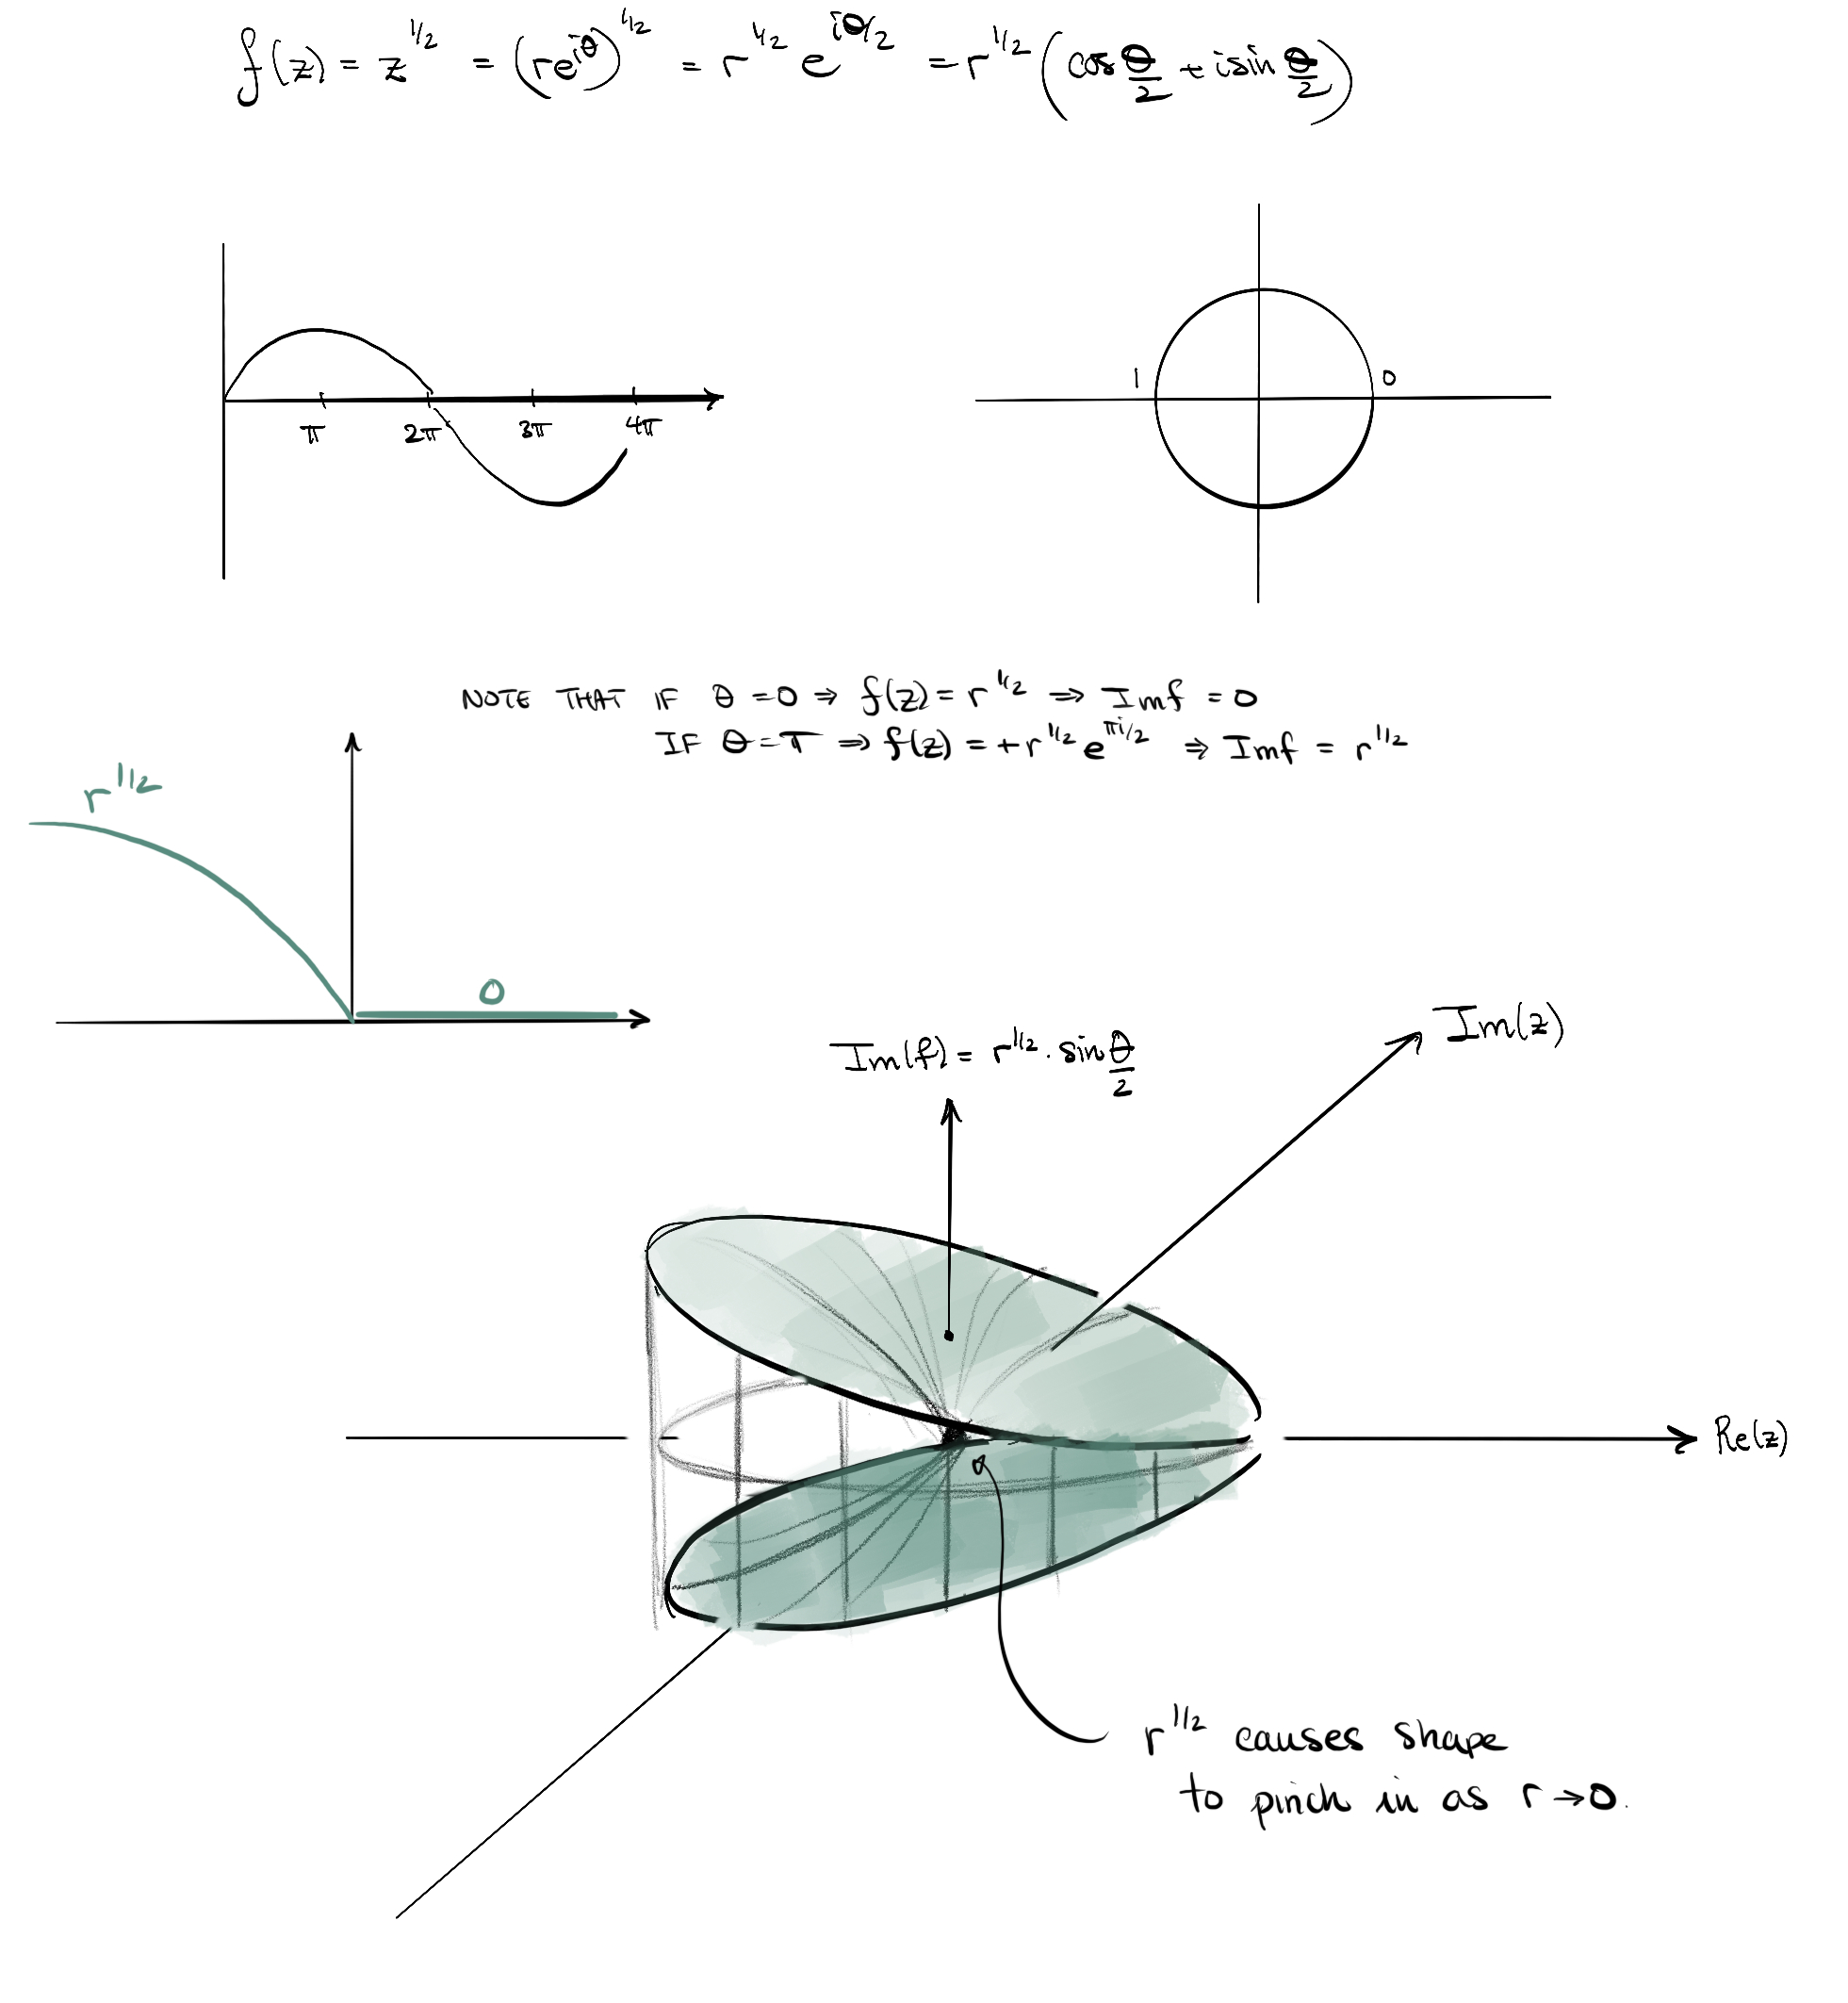
\includegraphics[width=\linewidth]{external/intro_squareroot.jpg}
\end{image}%
\tcblower
\end{figureptx}%
\end{enumerate}%
\end{divisionexercise}%
\begin{divisionexercise}{2}{A function with two branch points.}{}{ex-branch1}%
Consider the function \hyperref[eq-intro-twobranch]{({\xreffont\ref{eq-intro-twobranch}})}:%
\begin{equation*}
f(z) = (z + 1)^{1/2} (z - 1)^{1/2}.
\end{equation*}
%
\begin{enumerate}[font=\bfseries,label=(\alph*),ref=\alph*]%
\item{}Choose the branch cut from \(z = 1\) in the positive real direction. Choose the branch cut from \(z = -1\) in the negative real direction. Write either \(z = r_1 \e^{\im\theta_1}\) or \(z = r_2 \e^{\im\theta_2}\) for \(\theta_1\) and \(\theta_2\) defined as relative angles from the two branch points.%
\par
Show that: (i) when \(z = 1\) is encircled by a complete revolution, the function jumps in value by a factor of \(\e^{\im \pi}\); (ii) that there is a similar jump in value when \(z = -1\) is encircled. Finally what happens if (iii) \(z = 0\) is encircled?%
\par
Draw a picture of the final \(z\)-plane, showing the branch cuts.%
\par\smallskip%
\noindent\textbf{\blocktitlefont Solution}.\hypertarget{ex-branch1-3-2}{}\quad{}(i) We have that%
\begin{equation*}
f(z) = (r_1 r_2)^{1/2} \e^{\im \theta_1/2} \e^{\im \theta_2/2}.
\end{equation*}
Let \(\theta_1 \in [0, 2\pi)\) be the angle about the point \(z = 1\). Similarly let \(\theta_2 \in [-\pi, \pi)\) be the angle about the point \(z = -1\).%
\par
Considering firstly a revolution around \(z = 1\) (that does not also enclose \(z = -1\)). Let the initial point be denoted "A", with \(\theta_1 = 0, \theta_2 = 0\). And the final point be "B", with \(\theta_1 = 2\pi\) and \(\theta_2 = 0\).%
\par
Then%
\begin{equation*}
f(B) - f(A) = (r_1 r_2)^{1/2} \e^{2\pi\im/2} - (r_1 r_2)^{1/2} \e^0 = -2(r_1 r_2)^{1/2}.
\end{equation*}
so indeed there is a jump in the function about the branch cut along \(z > 1\).%
\par
(ii) We would similarly verify that for a contour around the branch point \(z = -1\) there is a jump. Let the initial point be denoted "A" with \(\theta_1 = \pi, \theta_2 = -\pi\). And the final point be "B" with \(\theta_1 = \pi, \theta_2 = \pi\). Then%
\begin{equation*}
f(B) - f(A) = (r_1 r_2)^{1/2} \e^{(\pi + \pi)\im/2} - (r_1 r_2)^{1/2} \e^{(\pi - \pi)\im/2} = -2(r_1 r_2)^{1/2}.
\end{equation*}
so indeed there is also a jump about the branch cut that runs \(z < -1\).%
\par
(iii) For the centre point, there are two cases to consider. The first case is if only \(z = 0\) is encircled and none of the other branch points. This was the situation originally envisioned in the question. For example, consider the circle of radius 1\slash{}2, i.e. \(z = (1/2) \e^{\im \theta}\) with \(\theta \in [0, 2\pi)\). You can verify that for this circle the start and end points agree.%
\par
If along with \(z = 0\), one of the branch points is encircled, then there would be a discontinuity. If both branch points are encircled, there is no discontinuity.%
\begin{figureptx}{Figure}{Branch cut configuration for the double square root. The original choice of branches is shown on top. Through the analysis, we see that a circle (i) around \(z = 1\) does not produce a discontinuity. Hence only the second picture of the cut arrangement is needed.}{ex-branch1-3-2-7}{}%
\begin{image}{0.15}{0.7}{0.15}{}%
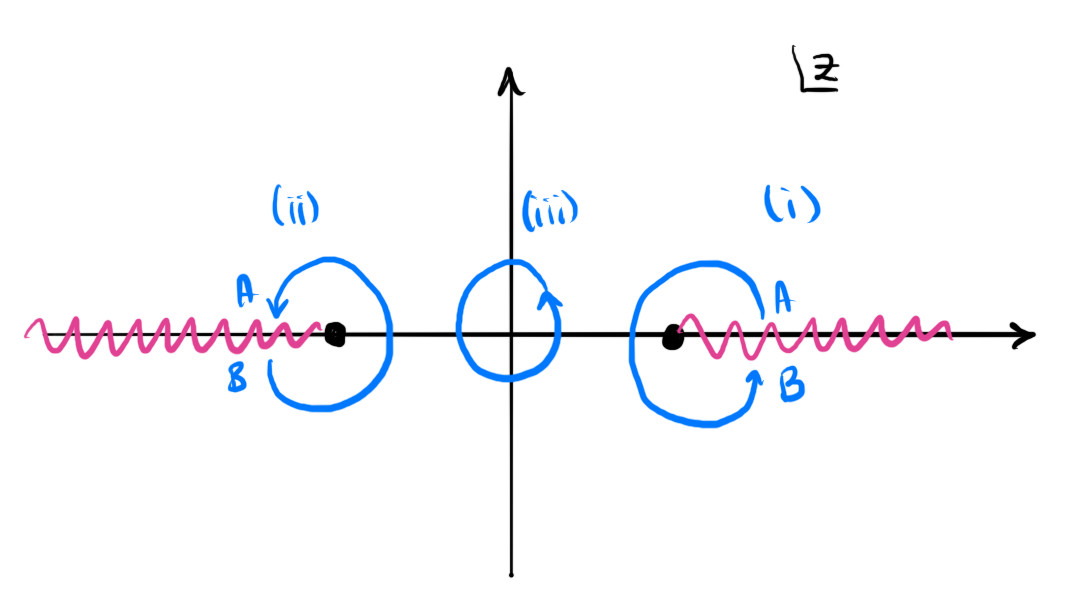
\includegraphics[width=\linewidth]{external/intro_doublesqrt_branch01.jpg}
\end{image}%
\tcblower
\end{figureptx}%
\item{}Consider now a branch cut from \(z = -1\) that tends in the positive real direction and the branch cut from \(z = 1\) tends in the positive real direction as well. Repeat the experiment above, considering (i)-(iii). Conclude that there is no jump in value along the region \(z > 1\) and hence the branch cuts required only extends between \(z = \pm 1\).%
\par
Draw a picture of the final \(z\)-plane, showing the branch cuts.%
\par\smallskip%
\noindent\textbf{\blocktitlefont Solution}.\hypertarget{ex-branch1-4-2}{}\quad{}For this situation, we would define the ranges of \(\theta_1 \in [0, 2\pi)\) and \(\theta_2 \in [0, 2\pi)\). One main difference is the analysis around the point \(z = 1\). Consider the similar loop to the above with,%
\begin{equation*}
f(B) - f(A) = (r_1 r_2)^{1/2} \e^{(2\pi + 2\pi)\im/2} - (r_1 r_2)^{1/2} \e^{(0 + 0)\im/2} = 0,
\end{equation*}
so in this case, notice that there is no jump due to the fact the total variation of angle is \(2 \pi + 2\pi\).%
\par
In essence, because both branch cuts are running in the positive real direction, when we orbit across \(z > 1\), we jump through both branches, hence returning to the original. There is no required branch cut for \(z > 1\).%
\par
The analysis of parts (ii) and (iii) are identical, with the exception of the angle range. However, the final result, of whether there exists a jump is the same.%
\par
In the end, the final branch cut picture is shown in the figure below.%
\begin{figureptx}{Figure}{Branch cut configuration for the double square root}{ex-branch1-4-2-5}{}%
\begin{image}{0.15}{0.7}{0.15}{}%
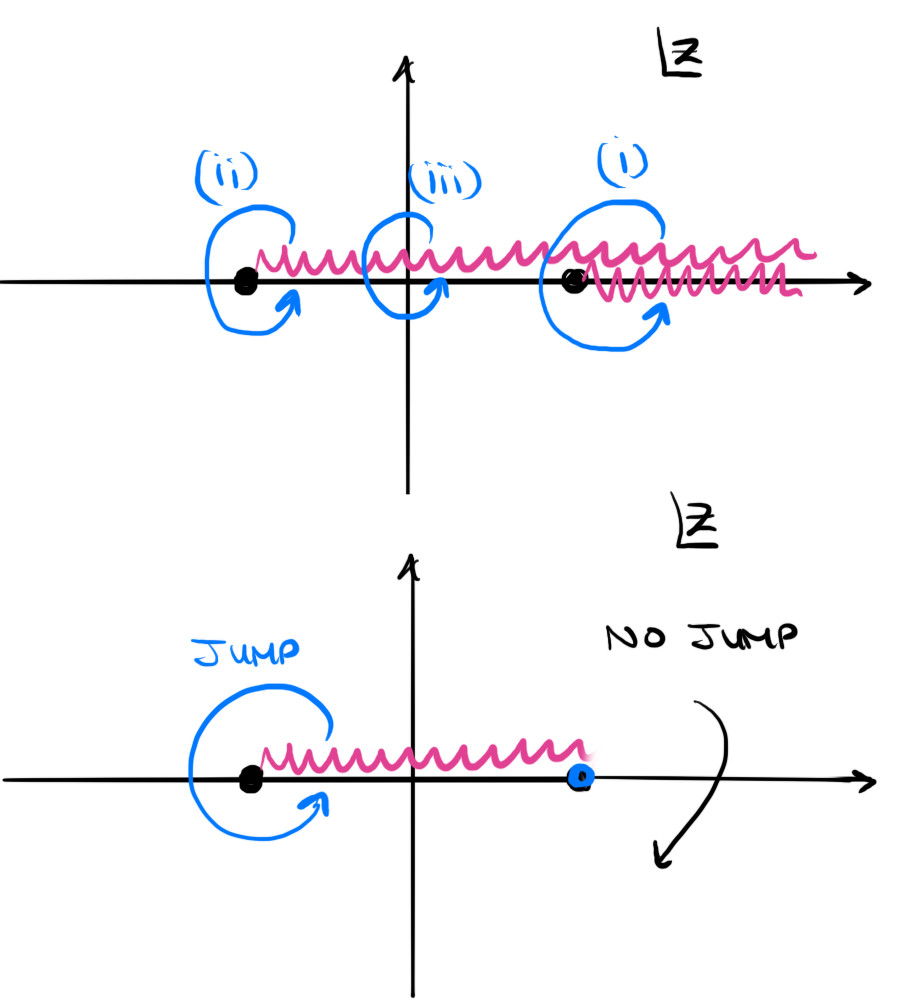
\includegraphics[width=\linewidth]{external/intro_doublesqrt_branch02.jpg}
\end{image}%
\tcblower
\end{figureptx}%
\item{}(Challenging). If you consider a plot of \((x, y, \Re f(x + \im y))\) or \((x, y, \Im f(x + \im y))\), what will the Riemann surface look like? You can attempt to plot this using any tool.%
\par\smallskip%
\noindent\textbf{\blocktitlefont Solution}.\hypertarget{ex-branch1-5-2}{}\quad{}This is certainly not an easy function to imagine! There are two features you may want to keep in mind. First, in examining the imaginary part of the function, if \(z > 1\) on the real axis, then the imaginary part is zero. Second, if \(z < -1\) on the real axis, then again the function is zero. Finally, for the case of the branch selection in part (b), the there is a cut along \([-1, 1]\). A generated plot is shown below for the imaginary part.%
\begin{figureptx}{Figure}{The imaginary part of \(f(z) = (z-1)^{1/2}(z +1)^{1/2}\)}{ex-branch1-5-2-2}{}%
\begin{image}{0.15}{0.7}{0.15}{}%
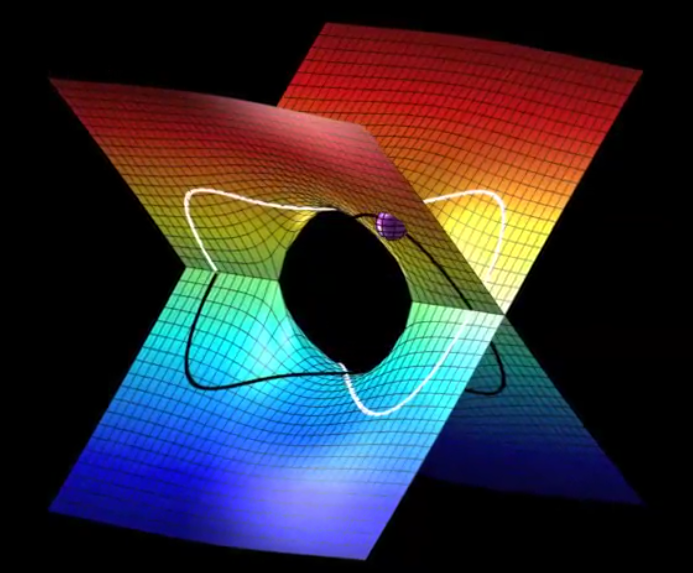
\includegraphics[width=\linewidth]{external/intro_doublesqrt_surf.png}
\end{image}%
\tcblower
\end{figureptx}%
\end{enumerate}%
\end{divisionexercise}%
\begin{divisionexercise}{3}{Branch cuts of the complex logarithm.}{}{ex-log}%
Consider the complex logarithm as defined in \hyperref[eqn-intro-complex-log]{({\xreffont\ref{eqn-intro-complex-log}})}.%
\begin{enumerate}[font=\bfseries,label=(\alph*),ref=\alph*]%
\item{}Explain why there must be a branch cut imposed, originating from the branch point at \(z = 0\).%
\par\smallskip%
\noindent\textbf{\blocktitlefont Solution}.\hypertarget{ex-log-3-2}{}\quad{}The logarithm will have a jump in the imaginary part every rotation of \(2\pi\) in the argument.%
\item{}Take the branch cut along the positive real axis. Do your best to draw the Riemann surface (consisting of the distinct Riemann sheets) of the logarithm, as visualised in the space \((x, y, \Im f(x + \im y))\).%
\par\smallskip%
\noindent\textbf{\blocktitlefont Solution}.\hypertarget{ex-log-4-2}{}\quad{}\begin{figureptx}{Figure}{The imaginary part of \(f(z) = \log z\).}{ex-log-4-2-1}{}%
\begin{image}{0}{1}{0}{}%
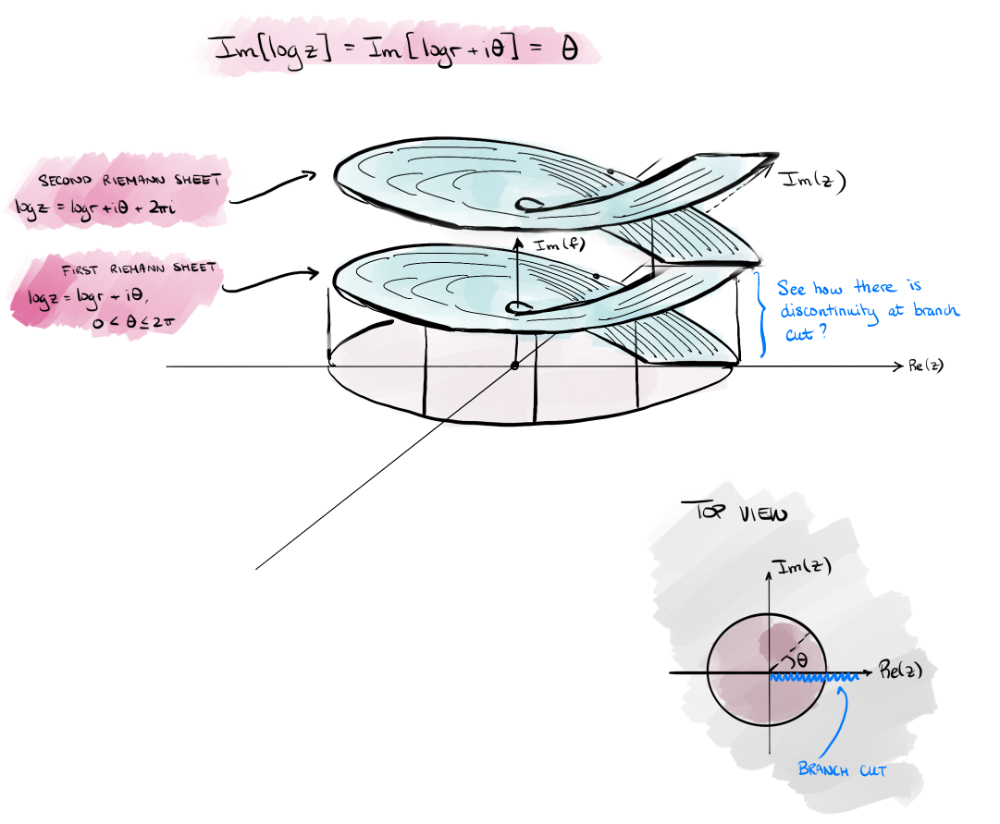
\includegraphics[width=\linewidth]{external/intro_log_surf.jpg}
\end{image}%
\tcblower
\end{figureptx}%
\item{}Again, you may find it useful to confirm your work above by plotting the function using a computational tool.%
\par\smallskip%
\noindent\textbf{\blocktitlefont Solution}.\hypertarget{ex-log-5-2}{}\quad{}There is a picture of the complex logarithm on \href{https://en.wikipedia.org/wiki/Complex_logarithm}{Wikipedia}.%
\end{enumerate}%
\end{divisionexercise}%
\end{exercises-section}
\end{chapterptx}
%
%
\typeout{************************************************}
\typeout{Chapter 2 Kinematics}
\typeout{************************************************}
%
\begin{chapterptx}{Chapter}{Kinematics}{}{Kinematics}{}{}{ch-chapter02-kinematics}
\renewcommand*{\chaptername}{Chapter}
\begin{introduction}{}%
Fluid \emph{kinematics} refers to the study of fluid motions without considering the associated forces (or energies) that cause such a fluid to move. In a nutshell, it relates to studying e.g. the general velocity and acceleration fields of a fluid, visualising the fluid trajectories, and so forth.%
\begin{figureptx}{Figure}{Eulerian description of flow from the \href{https://techtv.mit.edu/collections/ifluids/videos/32597-eulerian-and-lagrangian-descriptions-in-fluid-mechanics}{NCFMF video}.}{fig-euler-vid}{}%
\begin{image}{0.15}{0.7}{0.15}{}%
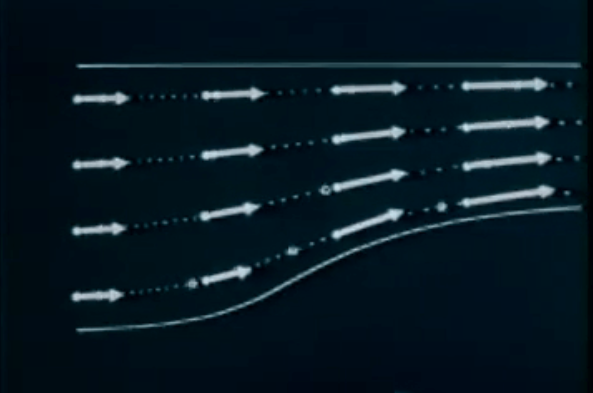
\includegraphics[width=\linewidth]{external/01_euler_trim.png}
\end{image}%
\tcblower
\end{figureptx}%
There are some unintuitive challenges when it comes to defining even the most basic quantities in fluid dynamics. Consider the following two thought experiments.%
\par
In the first experiment, we consider a tube filled with water, where the bottom is released at time \(t = 0\). One can imagine that the entire column of fluid will fall under the effect of gravity.%
\begin{figureptx}{Figure}{(a) Tube filled with fluid with a plate to be removed; (b) fluid falls under the effect of gravity with uniform acceleration everywhere.}{kinematic-tube01}{}%
\begin{image}{0.1}{0.8}{0.1}{}%
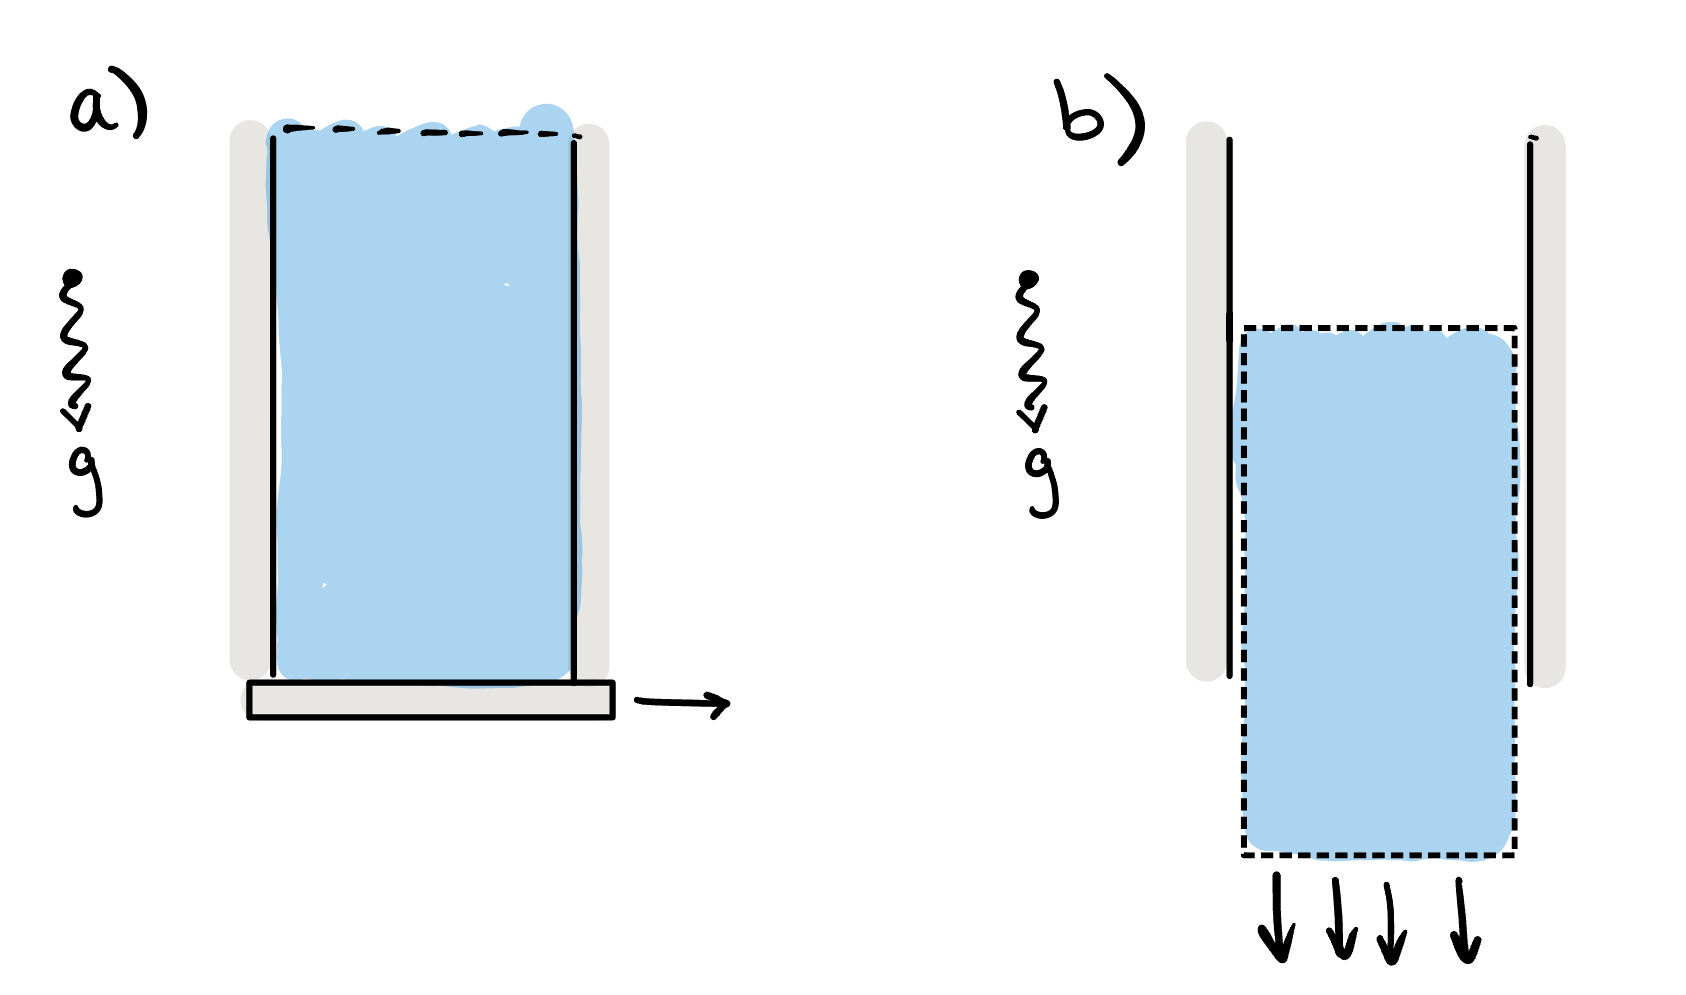
\includegraphics[width=\linewidth]{external/ch-chapter01-kinematics-tube01.png}
\end{image}%
\tcblower
\end{figureptx}%
Each particle within the fluid is accelerated downwards at a constant rate (gravity). Therefore the velocity of the fluid is given by \(\bu = (0, 0, -U(t)).\) In this case, we imagine that acceleration can be defined simply as the partial derivative, in time, of the velocity field, or%
\begin{equation*}
\ba
= \pd{\bu}{t} = (0, 0, -\dot{U}(t)) = (0, 0, -g),
\end{equation*}
where we have used the over-dot notation for a derivative in time.%
\par
However, consider now the second thought experiment of fluid being pumped through the vessel shown in the figure below. The fluid has reached a steady-state (so the streamlines of the flow, if you can imagine them, are constant and travelling from left-to-right).%
\begin{figureptx}{Figure}{Fluid pumped through a tube with variable cross-sectional area, \(A_1, A_2\) and corresponding velocities \(U_1, U_2\).}{kinematic-tube02}{}%
\begin{image}{0.1}{0.8}{0.1}{}%
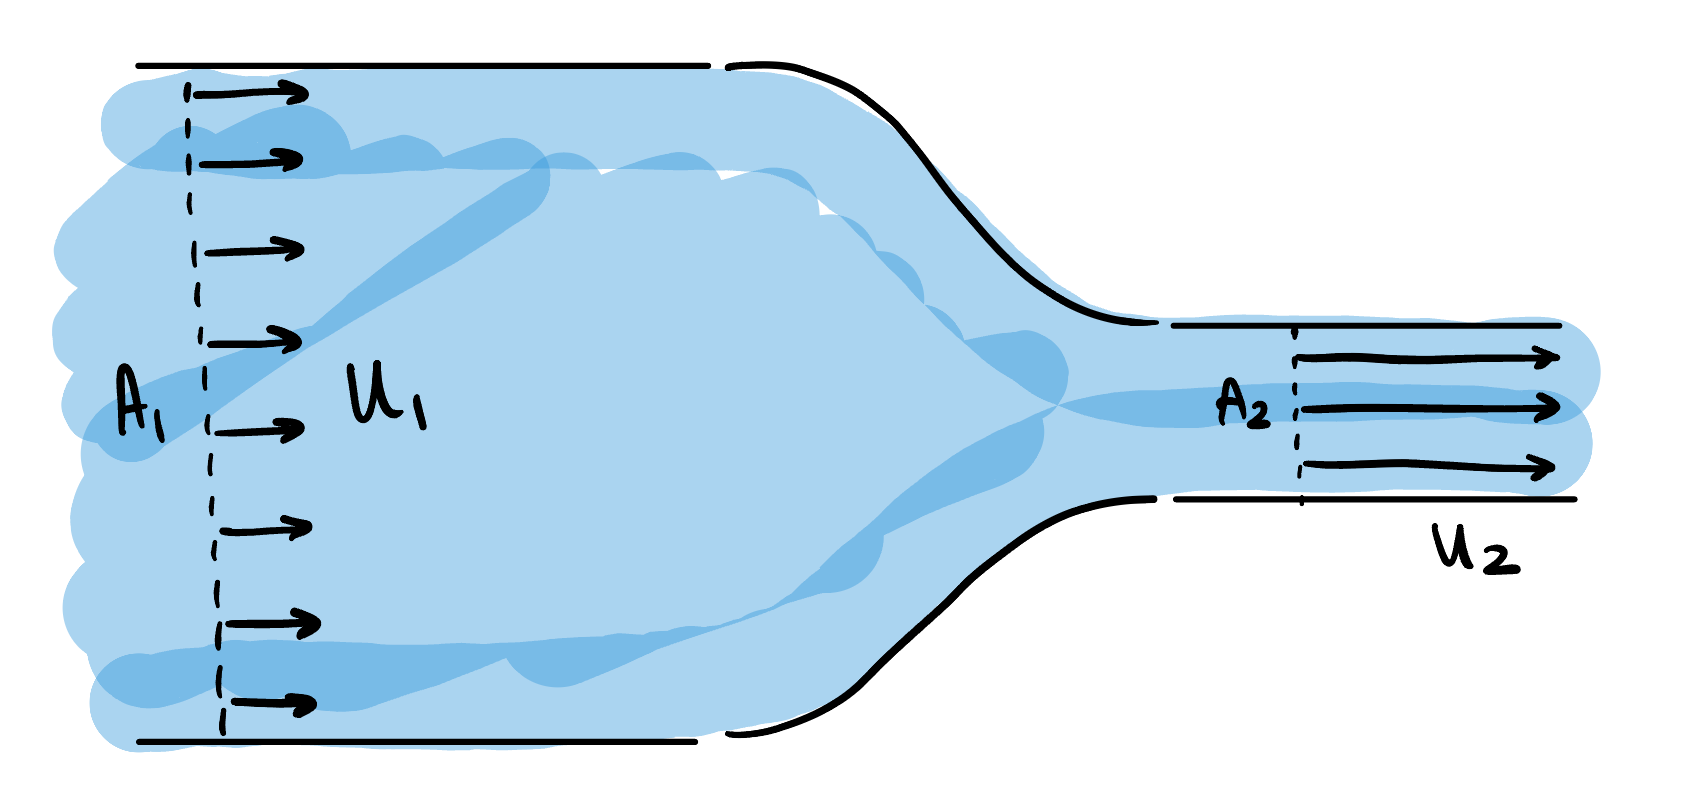
\includegraphics[width=\linewidth]{external/ch-chapter01-kinematics-tube02.png}
\end{image}%
\tcblower
\end{figureptx}%
Upstream of the bottleneck, the volume flowrate is equal to the velocity times area, or%
\begin{equation*}
\textrm{Upstream flow rate (area times velocity)} = A_1 U_1.
\end{equation*}
This is the amount of fluid that is flowing through a cross section of the pipe upstream. Similarly, we have%
\begin{equation*}
\textrm{Downstream flow rate (area times velocity)} = A_2 U_2.
\end{equation*}
%
\par
However, since mass must be conserved, that fact that there is a smaller cross-sectional area downstream must mean that the velocity is higher downstream. Therefore, \(U_2 > U_1\), and to achieve this, the fluid must therefore have been accelerated somewhere within the channel.%
\par
However, a thought to the situation might convince you that the velocity field in the channel is time-independent: it only changes as a function of its position and is therefore of the form \(\bu = \bu(\bx)\). Indeed, at every fixed point in the channel, the velocity \emph{at that point} is not changing in time. Therefore, if we use our previous definition that \(\ba = \dot{\bu}\) we see that the acceleration would be zero everywhere!%
\par
The crux of the issue, and the difference between the two thought experiments, is that velocity is both a function of space and time, i.e. \(\bu = \bu(\bx, t)\). The change in velocity (acceleration) can therefore derive from changes in \(\bu\) at fixed space and variable time; but also due to changes in \(\bu\) at fixed time and variable space. Disentangling this leads us to define the nature of Eulerian and Lagrangian coordinates, presented next.%
\end{introduction}%
%
%
\typeout{************************************************}
\typeout{Section 2.1 Eulerian and Lagrangian coordinates}
\typeout{************************************************}
%
\begin{sectionptx}{Section}{Eulerian and Lagrangian coordinates}{}{Eulerian and Lagrangian coordinates}{}{}{sec-eulerlagrang}
\begin{introduction}{}%
There are essentially two natural ways to think of motion in a fluid. We can imagine positioning ourselves at a fixed point in space, \(\bx = (x, y, z)\). At this point, we then attempt to measure a fluid quantity such as the density, \(\rho(\bx, t)\), or temperature, \(T(\bx, t)\). This is essentially the \emph{Eulerian frame}. One can imagine, for example, fixing sensor station into the ocean bottom, and obtaining measurements of the water temperature.%
\begin{figureptx}{Figure}{(a) The Eulerian interpretation; (b) the Lagrangian interpretation.}{sec-eulerlagrang-2-2}{}%
\begin{image}{0}{1}{0}{}%
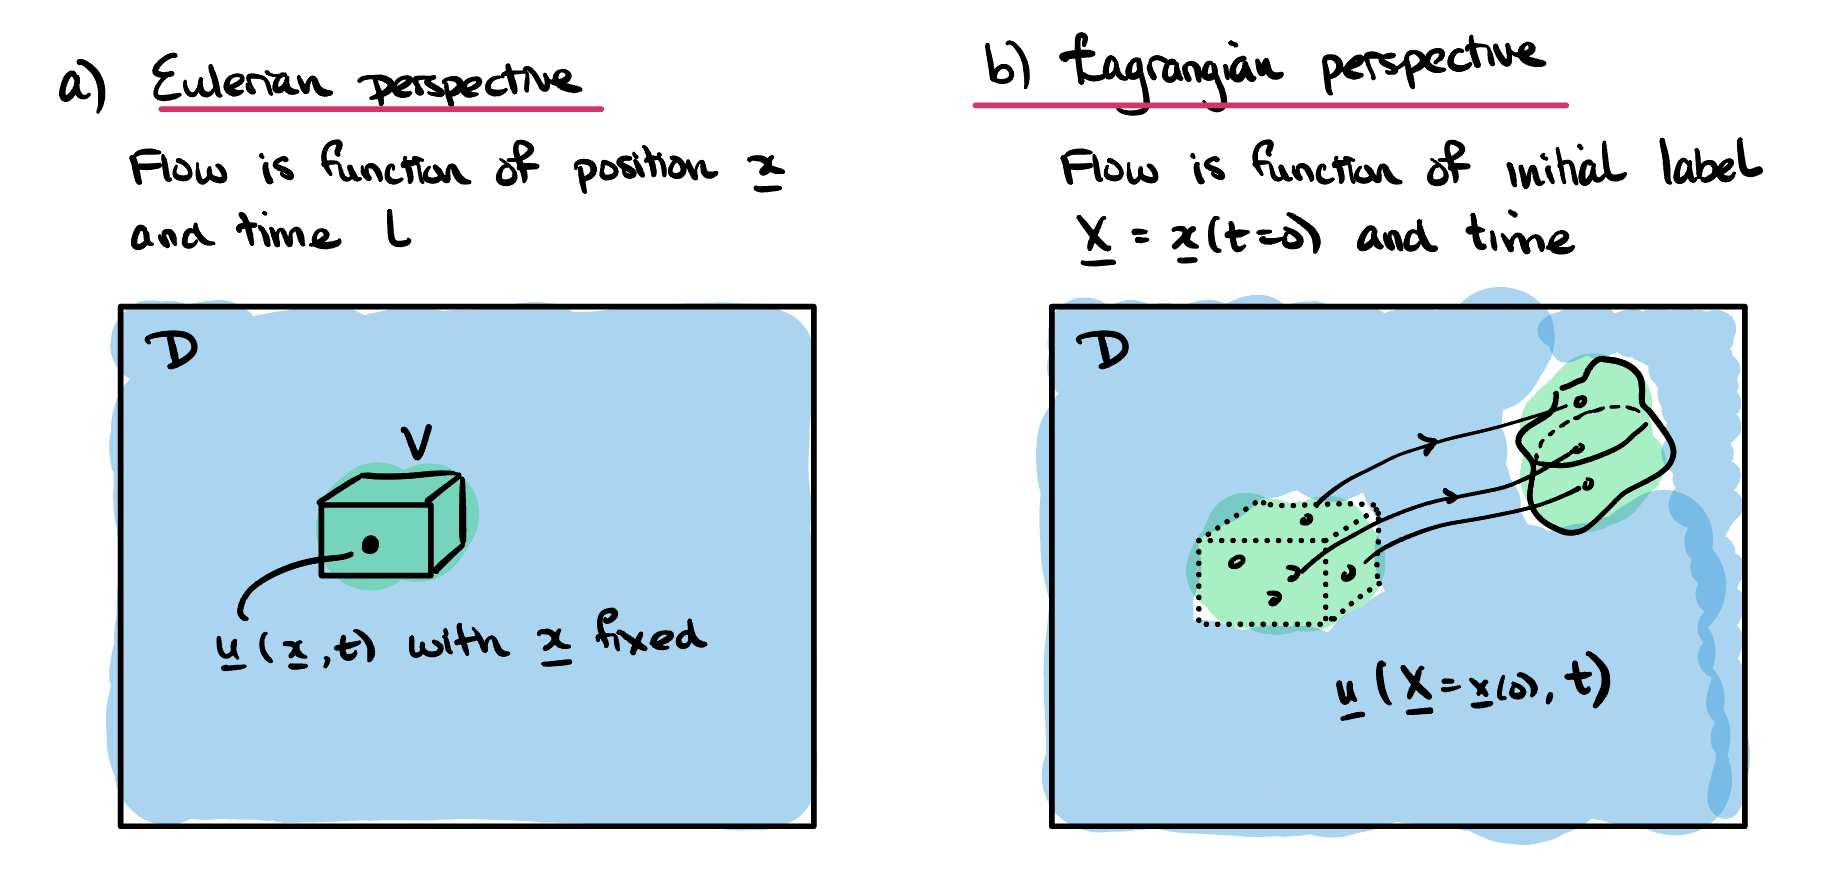
\includegraphics[width=\linewidth]{external/ch-chapter01-kinematics-euler-vs-lagrange.png}
\end{image}%
\tcblower
\end{figureptx}%
Alternatively, we can imagine tracking of a single fixed particle (or a fluid element) within the flow. The particle begins at some position. Let us define a label to describe the particle's initial position. For example, if the particle's position is given by%
\begin{equation*}
(x, y, z) = (x_1(t), y_1(t), z_1(t)),
\end{equation*}
we can define the corresponding \emph{Lagrangian label} as%
\begin{equation*}
\bX = (X, Y, Z) = (x_1(0), y_1(0), z_1(0)).
\end{equation*}
We then ask for the corresponding measurement of the fluid quantity that corresponds to the label \(\bX\). For example, this is equivalent to tagging a free-floating buoy in the ocean with the label \(\bX\), then measuring the temperature of the water as the buoy drifts in the ocean. This Lagrangian temperature could be written \(\mathcal{T}(\bX, t),\) where \(\bX\) is simply a fixed quantity for the particular buoy.%
\par
We are now in a position to define the Eulerian velocity field of a fluid.%
\begin{definition}{Definition}{}{def-velocity}%
The Eulerian velocity \(\bu(\bx,t)\) is the velocity of the fluid at the point with spatial coordinates \(\bx\) at time \(t\). Note that, in physical terms this velocity is the average velocity at the time \(t\) of the fluid particles (e.g. molecules, ions) in a small box centred on the point \(\bx\). See also \hyperref[rem-continuum]{Remark~{\xreffont\ref{rem-continuum}}} for a discussion of the continuum assumption.%
\end{definition}
It will be useful to introduce the concept of steady flow.%
\begin{definition}{Definition}{}{def-steady-flow}%
A velocity field \(\bu\) is defined as steady if it can be written \(\bu=\bu(\bx)\).%
\end{definition}
Note that steady flow does not mean that the fluid particles are not moving. It simply means that at a fixed point in space, the Eulerian velocity does not change in time. The Lagrangian velocity of a fluid particle will generally change in time, even in a steady flow.%
\par
A simple example of the conversion between the Eulerian and Lagrangian reference frames is in \hyperlink{ex-eulerian-lagrangian}{Exercise~{\xreffont 2.3.3}}.%
\end{introduction}%
%
%
\typeout{************************************************}
\typeout{Subsection 2.1.1 The convective derivative}
\typeout{************************************************}
%
\begin{subsectionptx}{Subsection}{The convective derivative}{}{The convective derivative}{}{}{subsec-laglabel}
Let us now be more specific. We wish to consider how different quantities in our flow changes with time, but the matter is made complicated by the two above perspectives (fixed or following the flow).%
\par
Again, let us consider a scalar property of the fluid (for example, its density, temperature, velocity component, pressure, etc.), and let us suppose that this quantity is a function of both position, \(\bx\), and time, \(t\), and denote it by \(f(\bx, t)\). This is the \emph{Eulerian description} of the property since it is defined by specifying a fixed position in space. Fixing \(\bx\) and then measuring \(f\) is akin to standing in the fluid at a fixed location and measuring the property value in time.%
\par
We can alternatively write the property by its Lagrangian description. That is, given a label \(\bX\), we obtain the current position of the particle associated with this label, \(\bx(\bX,
t)\), then obtain its property value. This we can write as the following:%
\begin{equation*}
F(\bX, t) \equiv f(\bx(\bX, t), t).
\end{equation*}
Now, fixing \(\bX\) and changing \(t\) corresponds to tracking the scalar property at a material point in the flow, or, equivalently, how \(f\) changes as we move with the particle along the deforming fluid.%
\par
There are thus two ways of considering time derivatives.%
\begin{definition}{Definition}{}{def-eulerlag}%
We use the normal partial derivative notation to refer to an \emph{Eulerian time derivative}, considered at a fixed point in space:%
\begin{equation*}
\pd{}{t} \equiv \pd{}{t} \biggr\rvert_{\bx} = \text{rate of change with $\bx$ held
constant}.
\end{equation*}
%
\par
On the other hand, the \emph{Lagrangian time derivative} is defined at a fixed material point in the fluid.%
\begin{equation*}
\DD{}{t} \equiv \pd{}{t} \biggr\rvert_{\bX} = \text{rate of change with $\bX$ held
constant}.
\end{equation*}
We often refer to the Lagrangian time derivative as the \emph{convective derivative} or the \emph{material derivative}.%
\end{definition}
\begin{remark}{Remark}{}{subsec-laglabel-7}%
The reason why the above derivatives are introduced is because, for the purpose of much of fluid dynamics, it is easier to work with Eulerian coordinates and quantities. However, for the purpose of deriving many governing equations, it turns out to be much easier to work with Lagrangian variables. This is because physical forces act on physical particles, or material elements, of the fluid.%
\end{remark}
The natural question is how the two derivatives relate to one another. This is given by the following theorem.%
\begin{theorem}{Theorem}{The material\slash{}convective derivative.}{}{thm-material-derivative}%
The \emph{material or convective derivative} can be defined in terms of Eulerian derivative in the following way:%
\begin{equation}
\DD{}{t} = \pd{}{t} + (\bu \cdot \nabla).\label{eqn-DDt}
\end{equation}
%
\end{theorem}
\begin{proof}{Proof}{}{thm-material-derivative-3}
This is a result of the chain rule. For a scalar function \(f = f(\bx, t)\), we have the fact that%
\begin{align*}
\DD{f}{t} &= \DD{t}{t} \pd{f}{t} + \DD{x}{t}\cdot \nabla f \\
&= \pd{f}{t} + \bu \cdot \nabla f. 
\end{align*}
%
\end{proof}
The proof to \hyperref[thm-material-derivative]{Theorem~{\xreffont\ref{thm-material-derivative}}} seems to use magic vector operations! In \hyperlink{ex-material-derivative}{Exercise~{\xreffont 2.3.2}}, we ask you to check this more carefully by expanding the vector operations explicitly.%
\par
We can now apply the above result to the question of how to calculate the acceleration within the fluid (more specifically, we are enquiring about the acceleration of a volume or particle within the fluid). The acceleration is given by the convective or material derivative of the velocity:%
\begin{equation}
\ba \equiv \DD{\bu}{t} = \pd{\bu}{t} + (\bu \cdot \nabla) \bu.\label{eqn-accel}
\end{equation}
You will practice using this formula in \hyperlink{ex-eulerian-lagrangian2}{Exercise~{\xreffont 2.3.4}} of the problem set.%
\begin{remark}{Remark}{Vector gradient.}{remark-vector-gradient}%
In the formula for the acceleration in \hyperref[eqn-accel]{({\xreffont\ref{eqn-accel}})}, the quantity%
\begin{equation*}
\nabla \bu
\end{equation*}
appears. This is a tensor (matrix). One mustn't be too intimidated as it is just a convenient notation.%
\par
It is worth considering what this must be by considering each individual element of the acceleration. The acceleration is calculated simply by taking the velocity,%
\begin{equation*}
\bu = (u, v, w) = (u_1, u_2, u_3). 
\end{equation*}
and working out the material derivative for each individual component. So we have%
\begin{equation}
\DD{u_i}{t} = \pd{u_i}{t} + \bu \cdot \nabla u_i.\label{eqn-material-deriv-ui}
\end{equation}
So the above gives each of the three components of \(\DD{\bu}{t}\).%
\par
You may prefer to see the above written in terms of the notation for \(\bu = (u, v, w)\), so it is%
\begin{align*}
\DD{u}{t} \amp= u_t + (u u_x + v u_y + w u_z)\\
\DD{v}{t} \amp= v_t + (u v_x + v v_y + w v_z)\\
\DD{w}{t} \amp= w_t + (u w_x + v w_y + w w_z)
\end{align*}
%
\par
You can also re-arrange the above in something closer to "matrix" form. So%
\begin{equation*}
\DD{\bu}{t} = \pd{}{t}(u, v, w) + (u, v, w) \cdot \begin{pmatrix} \nabla u \\ \nabla v \\ \nabla w\end{pmatrix},
\end{equation*}
and where the last quantity corresponds to%
\begin{equation}
\nabla \bu \equiv \begin{pmatrix} \nabla u \\ \nabla v \\ \nabla w\end{pmatrix} = 
\begin{pmatrix}
u_x & u_y & u_z \\
v_x & v_y & v_z \\
w_x & w_y & w_z 
\end{pmatrix}.\label{eqn-grad-bu}
\end{equation}
And hence the vector gradient can be defined as a matrix, where each row of the matrix is the gradient of the elements of the vector.%
\par
The author's opinionated note it is that it is easier simply to remember that the material derivative is applied via \hyperref[eqn-material-deriv-ui]{({\xreffont\ref{eqn-material-deriv-ui}})} then it is to try and untangle the multiplication of matrix via \hyperref[eqn-grad-bu]{({\xreffont\ref{eqn-grad-bu}})}.%
\end{remark}
\end{subsectionptx}
\end{sectionptx}
%
%
\typeout{************************************************}
\typeout{Section 2.2 Examples and flow visualisation}
\typeout{************************************************}
%
\begin{sectionptx}{Section}{Examples and flow visualisation}{}{Examples and flow visualisation}{}{}{sec-flowexamples}
\begin{introduction}{}%
There are different ways to visualise the dynamics of a fluid. Given the velocity, \(\bu(\bx,
t)\), we can plot a vector field at each point in space, and at a fixed moment in time. Little arrows are used to indicate the direction and the length of the arrow can be chosen to represent the magnitude. Joining these up at a fixed moment in time into smooth curves gives the \emph{streamlines} of the flow. This is often the easiest type of visualisation to perform mathematically, but the hardest experimentally.%
\par
Another representation of the flow is using \emph{particle paths} or \emph{pathlines}. Given a point and time, the particle path is the trajectory that would result if a particle were dropped into the flow at that chosen point and time. It is thus found by solving an equation where at every point on the trajectory, the particle's velocity is the specified velocity of the fluid.%
\par
A third representation is a \emph{streakline}. If dye were continuously released into a fluid from a fixed chosen point, the streakline at a given time is the line that would be made by the dye. It is thus found by finding the current position of those particles whose pathline has visited the chosen point at any past time. This is often the easiest type of visualisation to perform experimentally, but the hardest to perform mathematically.%
\par
Note that in a steady flow, the streamlines, pathlines and streaklines all coincide. However, in an unsteady flow, they are all different. In \hyperlink{ex-video-flow-visualisation}{Exercise~{\xreffont 2.3.1}} you will study a video showing this concept.%
\end{introduction}%
%
%
\typeout{************************************************}
\typeout{Subsection 2.2.1 Definitions of streamlines, pathlines, streaklines}
\typeout{************************************************}
%
\begin{subsectionptx}{Subsection}{Definitions of streamlines, pathlines, streaklines}{}{Definitions of streamlines, pathlines, streaklines}{}{}{sec-flowexamples-3}
In the definition below, we define these concepts more concretely.%
\begin{definition}{Definition}{Particle streamlines.}{def-streamline}%
Consider a fixed time, \(t = t_1\).%
\par
Select an initial point, \(\bx_1\) at this time.%
\par
The \emph{streamline}, \(\bx = \bx(s)\) through the above point is given by solving the parametric equation%
\begin{equation*}
\dd{\bx}{s} = \bu(\bx(s), t_1), \quad \text{with $\bx(s = 0) = \bx_1$,}
\end{equation*}
where \(s\) is a parameter along the streamline. Choosing a variety of different initial points, \(\bx_1\), and solving the above equation gives a family of streamlines at time \(t_1\).%
\end{definition}
Basically, given a velocity field, we freeze time. The streamlines are those curves that are traced out by the velocity field in the "snapshot".%
\begin{definition}{Definition}{Pathline or particle path.}{def-particle-path}%
Consider now a particle that begins at the location \(\bx_2\) at time \(t = 0\).%
\par
We consider the \emph{partical path} or \emph{pathline} of the particle, given by the curve \(\bx = \bx(t)\) and found by solving the equation%
\begin{equation*}
\dd{\bx}{t} = \bu(\bx(t), t), \quad \text{with $\bx(0) = \bx_2$.}
\end{equation*}
Choosing a variety of initial points, \(\bx_2\), yields a family of pathlines.%
\end{definition}
The pathline or particle path from an initial point is what we would physically expect if we were to dye the point with a colour and follow the dye colour as time increases.%
\begin{definition}{Definition}{Streakline.}{def-streakline}%
Consider now fixing a location \(\bx_3\).%
\par
The \emph{streakline} for a point \(\bx_3\) is given by solving the equation%
\begin{equation*}
\dd{\bx}{t} = \bu(\bx(t), t), \qquad \textrm{with $\bx(t_3) = \bx_3$},
\end{equation*}
for a variety of values of \(t_3\). This gives the current position of all particles that have passed through the point \(\bx_3\) at any time \(t_3\) in the past.%
\end{definition}
If it is the case that the velocity is time independent, i.e. \(\bu = \bu(\bx)\), then the three above definitions coincide.%
\par
You will practice the theory of these concepts in \hyperlink{ex-particle-paths-streamlines}{Exercise~{\xreffont 2.3.5}} and do a worked example in \hyperlink{ex-streamlines-pathlines-streaklines}{Exercise~{\xreffont 2.3.6}} of the problem set.%
\end{subsectionptx}
%
%
\typeout{************************************************}
\typeout{Subsection 2.2.2 Examples of streamlines, pathlines, and streaklines}
\typeout{************************************************}
%
\begin{subsectionptx}{Subsection}{Examples of streamlines, pathlines, and streaklines}{}{Examples of streamlines, pathlines, and streaklines}{}{}{subsec-examples-streamlines}
Let us practice these concepts.%
\begin{example}{Example}{Stagnation point flow.}{subsec-examples-streamlines-3}%
Consider a fluid described by the two-dimensional velocity field%
\begin{equation*}
\bu(\bx, t) = (x, -y, 0).
\end{equation*}
Derive and plot the streamlines of the flow. Discuss what occurs with particle paths and streaklines.%
\par\smallskip%
\noindent\textbf{\blocktitlefont Solution}.\hypertarget{subsec-examples-streamlines-3-3}{}\quad{}There are many online applications, such as \href{https://www.desmos.com/calculator/yhubcn7dij}{this one} that will allow you plot a two-dimensional direction field. It is also good to do it yourself by hand.%
\begin{figureptx}{Figure}{An example of a direction field}{subsec-examples-streamlines-3-3-2}{}%
\begin{image}{0.05}{0.9}{0.05}{}%
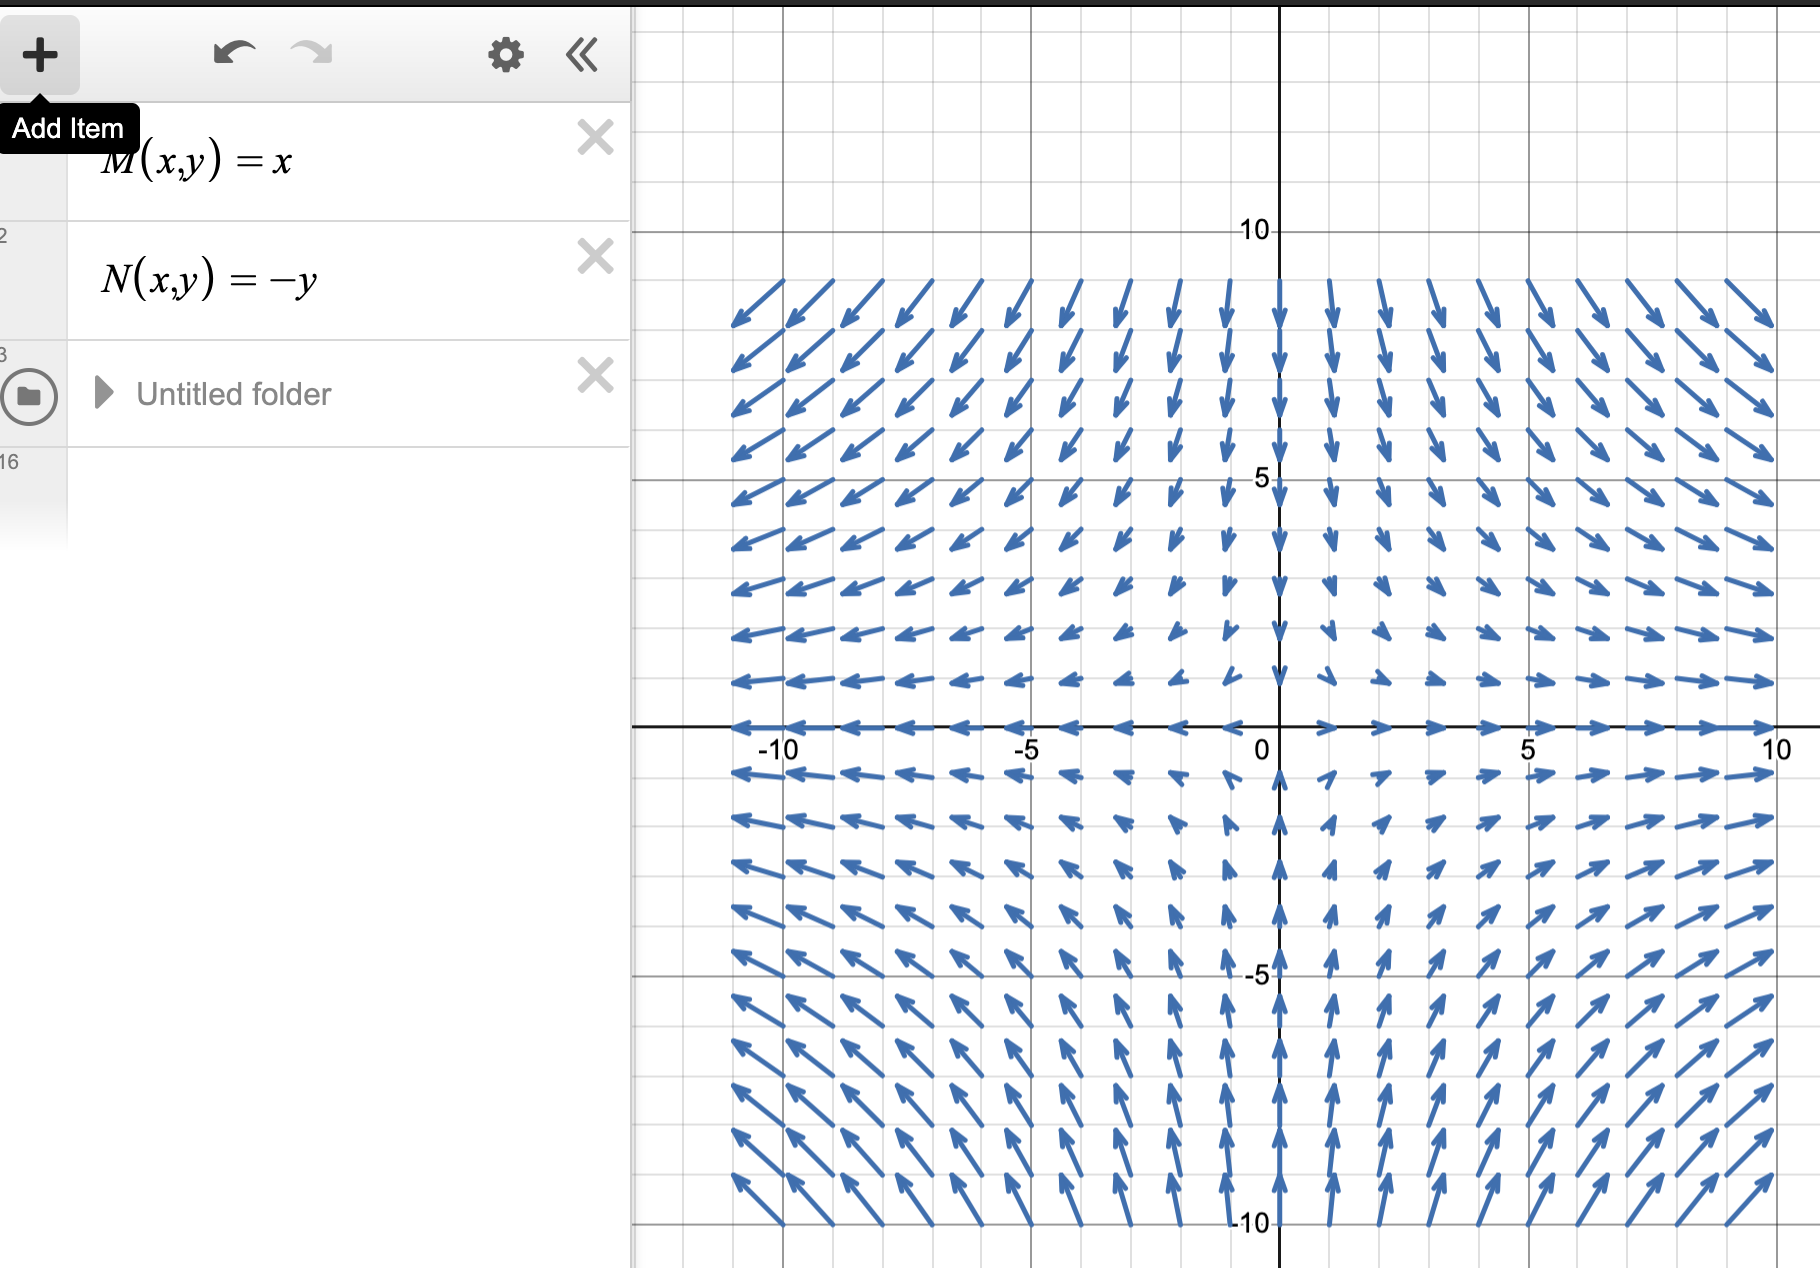
\includegraphics[width=\linewidth]{external/directionfieldexample.png}
\end{image}%
\tcblower
\end{figureptx}%
The streamlines follow from \hyperref[def-streamline]{Definition~{\xreffont\ref{def-streamline}}}. We seek to solve the equations%
\begin{align*}
\dd{x}{s} &= x, \\
\dd{y}{s} &= -y, \\
\dd{z}{s} &= 0. 
\end{align*}
Solving thus gives \(x = A \e^s, y = B\e^{-s}, z = C,\) for constants \(A, B, C\).%
\par
You can put initial conditions to determine the constant and plot the trajectories for different values of \(s\).%
\par
However, in this case, it is easier to remove the time-like variable, \(s\), entirely. Notice that%
\begin{equation*}
xy = AB = \textrm{constant}.
\end{equation*}
Therefore, the trajectories lie along hyperbolae.%
\par
Notice that in this case, the velocity field is time-independent, and therefore the particle paths coincide with the streamlines and streaklines.%
\par
For instance, the particle path through a particle at \(\bx_2 = (1, 1, 0)\) is given by (replacing \(s\) with \(t\)):%
\begin{equation*}
\bx(t) = (\e^t, \, \e^{-t}, \, 0).
\end{equation*}
Similarly, the \emph{streakline} through the point \((1, 1, 0)\) is precisely the set of points above.%
\end{example}
\begin{example}{Example}{Straight streamlines and circular pathlines.}{subsec-examples-streamlines-4}%
Consider the unsteady flow given by%
\begin{equation*}
\bu(\bx, t) = (\cos t, \sin t, 0)\text{.}
\end{equation*}
Plot the streamlines of the flow on the plane \(z = 0\), and also the particle trajectories. What occurs with the streaklines?%
\par\smallskip%
\noindent\textbf{\blocktitlefont Answer}.\hypertarget{subsec-examples-streamlines-4-3}{}\quad{}In this case, the velocity field is changing in time. Consider firstly the concept of the streamline in \hyperref[def-streamline]{Definition~{\xreffont\ref{def-streamline}}}.%
\par
We solve the governing equations for the streamlines \(\bx = \bx(s)\),%
\begin{equation*}
\dd{x}{s} = \cos t, \quad \dd{y}{s} = \sin t, \quad \dd{z}{s} = 0,
\end{equation*}
for fixed \(t\).%
\par
This gives%
\begin{equation*}
x(s) = A + s \cos t, \quad y(s) = B + \sin t, \quad z(s) = C,
\end{equation*}
for constants \(A, B, C\). Therefore the streamline are given by straight lines in the \((x, y)\) plane, if \(z = C\) is fixed.%
\par
Consider instead the definition of particle paths via \hyperref[def-particle-path]{Definition~{\xreffont\ref{def-particle-path}}}. We seek to solve%
\begin{equation*}
\dd{x}{t} = \cos t, \quad \dd{y}{t} = \sin t, \quad \dd{z}{t} = 0,
\end{equation*}
yielding%
\begin{equation*}
x(t) = A + \sin t, \quad y(t) = B - \cos t, \quad z(t) = C, 
\end{equation*}
for constants \(A, B, C\). Therefore, we see that the particle paths are closed circles (in the \(xy\)-plane) of unit radius encircling the point \((A, B, 0)\).%
\par
The fact that the streamlines are straight lines while the particle paths are circular can be visualised in \hyperref[fig-streamlines-example-02]{Figure~{\xreffont\ref{fig-streamlines-example-02}}}%
\begin{figureptx}{Figure}{Streamlines and particle paths}{fig-streamlines-example-02}{}%
\begin{image}{0.25}{0.5}{0.25}{}%
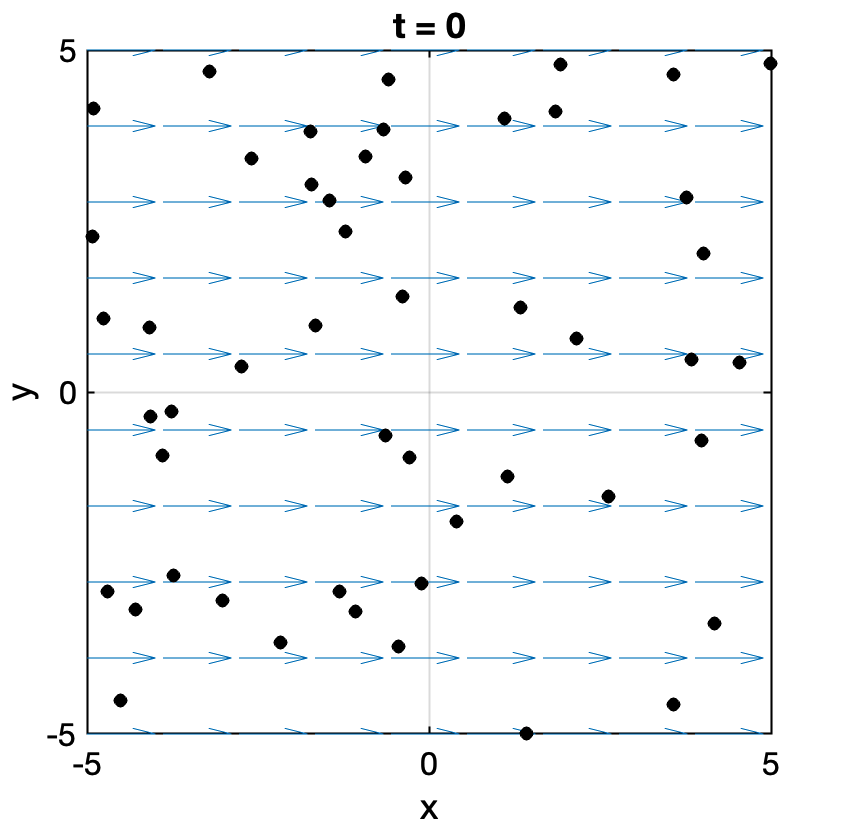
\includegraphics[width=\linewidth]{external/streamlines_example02.png}
\end{image}%
\tcblower
\end{figureptx}%
In this case, considering the streakline via \hyperref[def-streakline]{Definition~{\xreffont\ref{def-streakline}}}, we conclude that the streakline coincides with the particle path. Can you reason why this must be the case in this situation? What is necessary in order for this not to be true?%
\end{example}
\begin{example}{Example}{An oscillating hose\slash{}plate.}{subsec-examples-streamlines-5}%
Water flows out of an oscillating sprinkler head, held along the edge \(y = 0\), such that the velocity field produced is given by%
\begin{equation*}
\bu = [u_0 \sin[\omega(t - y/{v_0})], v_0],
\end{equation*}
where \(u_0\) and \(v_0\) are constants.%
\par
Determine the streamline that passes through the origin at \(t = 0\) and \(t = \pi/(2\omega)\).%
\par
Determine the pathline of the particle that was at the origin at \(t = 0\); at \(t = \pi/2\).%
\par
Qualitatively describe the shape of the streakline that passes through the origin?%
\par\smallskip%
\noindent\textbf{\blocktitlefont Answer}.\hypertarget{subsec-examples-streamlines-5-3}{}\quad{}\begin{figureptx}{Figure}{Isolated pathlines show that particles move along straight paths.}{fig-hose01}{}%
\begin{image}{0.1}{0.8}{0.1}{}%
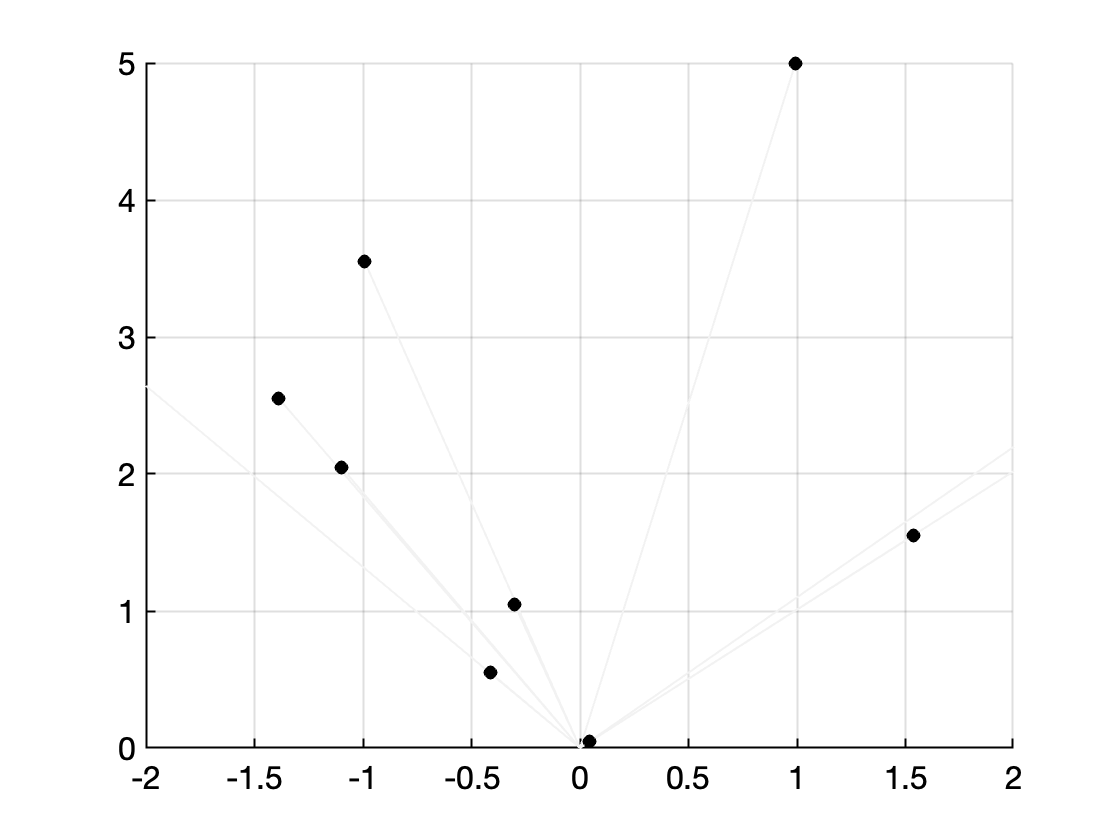
\includegraphics[width=\linewidth]{external/hose01.png}
\end{image}%
\tcblower
\end{figureptx}%
\begin{figureptx}{Figure}{However, viewed in terms of the streakline, the visible pattern is oscillatory.}{fig-hose02}{}%
\begin{image}{0.1}{0.8}{0.1}{}%
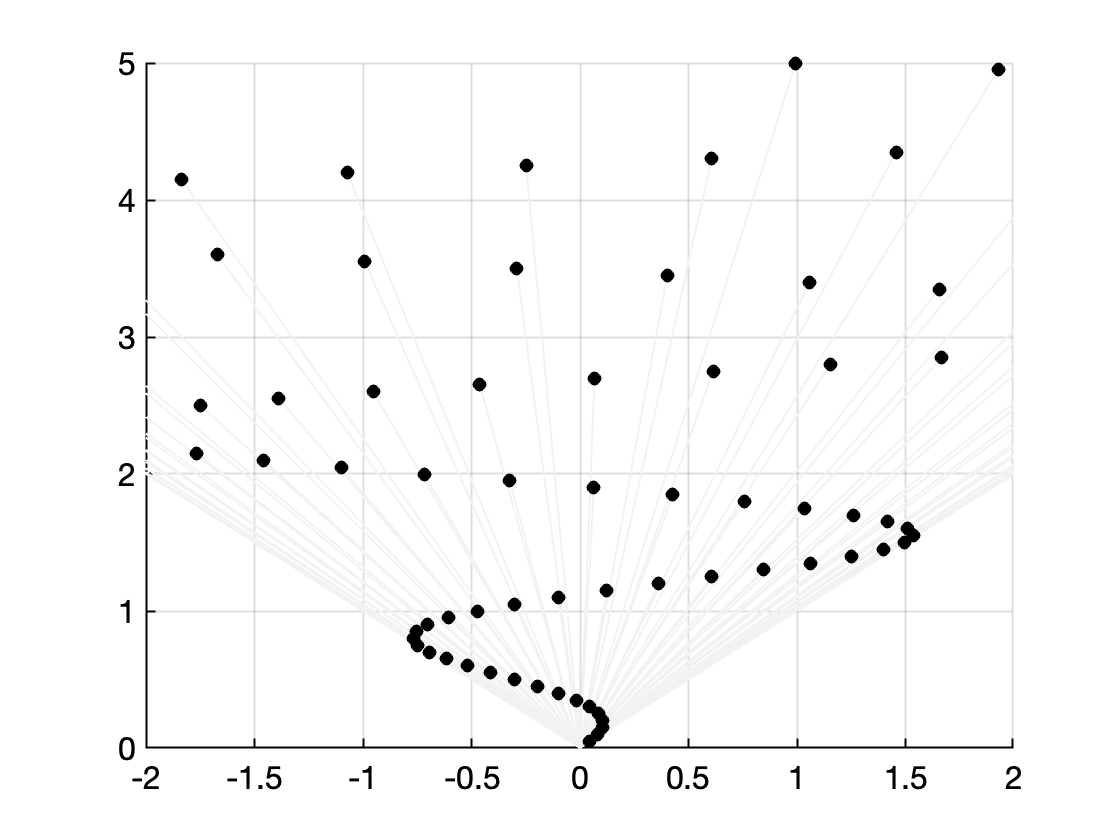
\includegraphics[width=\linewidth]{external/hose02.png}
\end{image}%
\tcblower
\end{figureptx}%
\end{example}
\end{subsectionptx}
\end{sectionptx}
%
%
\typeout{************************************************}
\typeout{Exercises 2.3 Exercises}
\typeout{************************************************}
%
\begin{exercises-section}{Exercises}{Exercises}{}{Exercises}{}{}{ws-kinematics}
\begin{introduction}{}%
The kinematics chapter covered the basic essentials about the measurement and computation of fluid velocities and acceleration. We examined the difference between Eulerian and Lagrangian coordinates and derivatives. Examples of streamlines and velocity fields were examined.%
\end{introduction}%
\begin{divisionexercise}{1}{Flow visualisation.}{}{ex-video-flow-visualisation}%
\href{https://techtv.mit.edu/collections/ifluids/videos/32598-flow-visualization}{Watch the first 13 and half minutes of the video "Flow visualisation" from the NCFMF archives}.%
\begin{enumerate}[font=\bfseries,label=(\alph*),ref=\alph*]%
\item{}Name a few ways in which a fluid flow can be visualised (i.e. how does one produce, in an experiment, such a visualisation?)%
\item{}Define, in words, what \emph{pathline}, \emph{streakline}, \emph{timeline}, and \emph{streamline} means. At 6:30, the author comments that "there is no way to make a streamline visible". Discuss this point.%
\item{}Give the example, shown in the video, where the pathline, streakline, and streamlines all coincide. Draw pictures to illustrate the concept.%
\item{}Give an example, shown in the video, where the pathline, streakline, and streamlines do not coincide. Draw pictures to illustrate the concept.%
\item{}In the video, an intuitive explanation is given for what it means for the velocity to be \emph{incompressible}. What is this explanation? (near 8:25)%
\end{enumerate}%
\end{divisionexercise}%
\begin{divisionexercise}{2}{Derivation of the material derivative.}{}{ex-material-derivative}%
Prove the Eulerian representation of the material derivative, as presented in \hyperref[thm-material-derivative]{Theorem~{\xreffont\ref{thm-material-derivative}}} by manually expanding the components of the function. That is, consider a scalar function \(f(\bx, t)\). Let the spatial coordinate follow \(\bx = \bx(\bX,t)\) and hence is defined by a specified material label \(\bX\). Then derive the identity for%
\begin{equation*}
\DD{f}{t} = \pd{f}{t} \biggr\rvert_{\bX},
\end{equation*}
according to \hyperref[def-eulerlag]{Definition~{\xreffont\ref{def-eulerlag}}}.%
\par\smallskip%
\noindent\textbf{\blocktitlefont Solution}.\hypertarget{ex-material-derivative-3}{}\quad{}This is the chain rule. Denote the three components of \(\bx = (x_1, x_2, x_3)\). Then we differentiate through both outer arguments of \(f\):%
\begin{align*}
\pd{f(\bx(\bX, t), t)}{t}\biggr\rvert_{\bX} &= \pd{f}{t}\biggr\rvert_{\bx} + \sum_{i=1}^3 \pd{x_i(\bX, t)}{t}\biggr\rvert_{\bX} \pd{f}{x_i} 
\end{align*}
%
\par
The factor,%
\begin{equation*}
\pd{x_i}{t}\biggr\rvert_{\bX} = \dd{x_i}{t} \equiv u_i,
\end{equation*}
corresponds to the velocity component in each direction. Then%
\begin{equation*}
\pd{f(\bx(\bX, t), t)}{t}\biggr\rvert_{\bX} = \pd{f}{t} + \bu \cdot \nabla f,
\end{equation*}
as desired.%
\end{divisionexercise}%
\begin{divisionexercise}{3}{Eulerian and Lagrangian descriptions.}{}{ex-eulerian-lagrangian}%
A velocity field is described in Eulerian terms in Cartesian coordinates by \(\mathbf{u}=(-y,x)\).%
\begin{enumerate}[font=\bfseries,label=(\alph*),ref=\alph*]%
\item{}What is the Lagrangian position of the particle that starts at the point \((x_0,y_0)\)? Describe its path. What is its velocity?%
\par\smallskip%
\noindent\textbf{\blocktitlefont Solution}.\hypertarget{ex-eulerian-lagrangian-3-2}{}\quad{}A particle moves with the velocity of the fluid. Then it must satisfy the equations%
\begin{equation*}
\dd{x}{t} = -y(t),\quad \dd{y}{t} = x(t)
\quad\Rightarrow\quad
\dd{^2x}{t^2} = -\dd{y}{t} = -x(t).
\end{equation*}
Trying solutions of the form \(x(t)=\e^{\lambda t}\) gives \(\lambda=\pm i\), so the general solution is%
\begin{equation*}
x(t) = Ae^{it}+Be^{-it},
\end{equation*}
or, equivalently,%
\begin{equation*}
x(t) = C\cos t + D\sin t,
\end{equation*}
where \(C\) and \(D\) are constants, and%
\begin{equation*}
y(t) =-\dd{x}{t}= C\sin t - D\cos t.
\end{equation*}
Setting \(x(0)=x_0\) and \(y(0)=y_0\) gives \(C=x_0\) and \(D=-y_0\), so%
\begin{equation*}
\bx(t) = (x_0\cos t - y_0\sin t, x_0\sin t + y_0\cos t).
\end{equation*}
This is a circular path of radius \(\sqrt{x_0^2+y_0^2}\) going anticlockwise around the origin. The velocity is%
\begin{equation*}
(x,y)(t) = (-x_0\sin t - y_0\cos t, x_0\cos t - y_0\sin t).
\end{equation*}
%
\item{}Express the position and velocity in polar coordinates. What do you notice?%
\par\smallskip%
\noindent\textbf{\blocktitlefont Solution}.\hypertarget{ex-eulerian-lagrangian-4-2}{}\quad{}The calculation works out more simply in polar coordinates; the velocity field is%
\begin{equation*}
\bu = r\be_\theta,
\end{equation*}
where \(\be_{\theta}\) is the angular unit vector given in \hyperref[eqn-appendix-polar-er-etheta]{({\xreffont\ref{eqn-appendix-polar-er-etheta}})}. Then the equation for particle paths is%
\begin{equation*}
\dd{r}{t} = 0,\quad\dd{r\theta}{t}= r\quad\Rightarrow\quad \dd{\theta}{t}=1.
\end{equation*}
Thus \(r(t)=r_0=\sqrt{x_0^2+y_0^2}\) and \(\theta(t)=\theta_0+t\), where \(\theta_0=\tan^{-1}(y_0/x_0)\). The velocity is \(\bu(t)=r_0\be_{\theta}(t)\).%
\end{enumerate}%
\end{divisionexercise}%
\begin{divisionexercise}{4}{Eulerian and Lagrangian descriptions.}{}{ex-eulerian-lagrangian2}%
A fluid flows through the nozzle shown from \(x=0\) to \(x=L\) with one-dimensional velocity%
\begin{equation*}
u=U\left(1+\frac{x}{L}\right)
\end{equation*}
in the \(x\)-direction, where \(U\) and \(L\) are constants. Note that, in reality the flow would be two- or three-dimensional, but we ignore this here for simplicity.%
 \begin{figureptx}{Figure}{Sketch of nozzle.}{fig-nozzle}{}%
\begin{image}{0.2}{0.6}{0.2}{}%
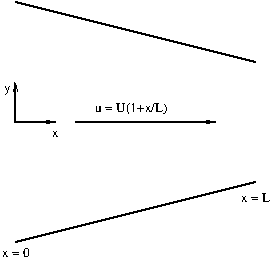
\includegraphics[width=\linewidth]{external/ch-chapter02-nozzle.png}
\end{image}%
\tcblower
\end{figureptx}%
\begin{enumerate}[font=\bfseries,label=(\alph*),ref=\alph*]%
\item{}What is the particle acceleration?%
\par\smallskip%
\noindent\textbf{\blocktitlefont Solution}.\hypertarget{ex-eulerian-lagrangian2-3-2}{}\quad{}%
\begin{align*}
\ba=&\DD{\bu}{t} \\
=& \pd{\bu}{t} + (\bu \cdot \nabla) \bu\\
=&0+\left(u\pd{u}{x}+v\pd{u}{y}+w\pd{u}{z}\right)\be_x
+\left(u\pd{v}{x}+v\pd{v}{y}+w\pd{v}{z}\right)\be_y
+\left(u\pd{w}{x}+v\pd{w}{y}+w\pd{w}{z}\right)\be_z\\
=& u\pd{u}{x}\be_x\\
= & U\left(1+\frac{x}{L}\right)\frac{U}{L}\be_x\\
= & \frac{U^2}{L}\left(1+\frac{x}{L}\right)\be_x
\end{align*}
%
\item{}If a particle starts at \(x=0\) at time \(t=0\), what is its position at time \(t\)?%
\par\smallskip%
\noindent\textbf{\blocktitlefont Solution}.\hypertarget{ex-eulerian-lagrangian2-4-2}{}\quad{}We have%
\begin{equation*}
\dd{x}{t}=u(x)=U\left(1+\frac{x}{L}\right).
\end{equation*}
Solving by separation of variables gives,%
\begin{align*}
&\int_0^x\frac{dx}{1+x/L}=\int_0^t U\,dt\\
\Rightarrow\quad& L\ln\left(1+\frac{x}{L}\right)=Ut\\
\Rightarrow\quad& x(t)=L\left(\e^{Ut/L}-1\right).
\end{align*}
%
\item{}What is its Lagrangian velocity as a function of time?%
\par\smallskip%
\noindent\textbf{\blocktitlefont Solution}.\hypertarget{ex-eulerian-lagrangian2-5-2}{}\quad{}The velocity is%
\begin{align*}
\dd{x}{t}=&\dd{}{t}\left(L\left(\e^{Ut/L}-1\right)\right)\\
=& L\frac{U}{L}\e^{Ut/L}\\
=& U\e^{Ut/L}.
\end{align*}
%
\item{}What is its Lagrangian acceleration as a function of time?%
\par\smallskip%
\noindent\textbf{\blocktitlefont Solution}.\hypertarget{ex-eulerian-lagrangian2-6-2}{}\quad{}The acceleration is%
\begin{align*}
\dd{^2x}{t^2}=&\dd{}{t}\left(U\e^{Ut/L}\right)\\
=& \frac{U^2}{L}\e^{Ut/L}.
\end{align*}
%
\item{}Write the Lagrangian velocity and acceleration as a function of \(x\). Compare with the corresponding Eulerian velocity and particle acceleration. What do you notice?%
\par\smallskip%
\noindent\textbf{\blocktitlefont Solution}.\hypertarget{ex-eulerian-lagrangian2-7-2}{}\quad{}The velocity is%
\begin{equation*}
U\e^{Ut/L}=U\left(1+\frac{x}{L}\right),
\end{equation*}
as expected. This is the same as the Eulerian velocity at the particle position. The acceleration is%
\begin{align*}
\frac{U^2}{L}\e^{Ut/L}=&\frac{U^2}{L}\left(1+\frac{x}{L}\right),
\end{align*}
which is the same as the particle acceleration, as expected from the defintion.%
\item{}How long does it take for a particle to travel from \(x=0\) to \(x=L\)?%
\par\smallskip%
\noindent\textbf{\blocktitlefont Solution}.\hypertarget{ex-eulerian-lagrangian2-8-2}{}\quad{}The particle reaches \(x=L\) when%
\begin{align*}
& L\left(\e^{Ut/L}-1\right)=L\\
\Rightarrow\quad& \e^{Ut/L}=2\\
\Rightarrow\quad& t=\frac{L}{U}\ln(2).
\end{align*}
%
\end{enumerate}%
\end{divisionexercise}%
\begin{divisionexercise}{5}{Particle paths and streamlines.}{}{ex-particle-paths-streamlines}%
\begin{enumerate}[font=\bfseries,label=(\alph*),ref=\alph*]%
\item{}Define the particle paths and streamlines for a velocity field \(\bu(\bx,t)\). When do these coincide?%
\par\smallskip%
\noindent\textbf{\blocktitlefont Answer}.\hypertarget{ex-particle-paths-streamlines-2-2}{}\quad{}Particle paths are the trajectories of individual fluid particles, which are found by solving the ODE%
\begin{equation*}
\dd{\bx}{t} = \bu(\bx,t).
\end{equation*}
Streamlines are curves that are instantaneously tangent to the velocity field, and therefore satisfy%
\begin{equation*}
\dd{\bx}{s} = \bu(\bx,t),
\end{equation*}
where \(s\) is a parameter along the streamline. The two coincide if the flow is steady, i.e. \(\bu(\bx,t)=\bu(\bx)\).%
\item{}Show that a quantity \(f(\bx,t)\) is preserved following the flow if%
\begin{equation*}
\DD{f}{t}=\pd{f}{t}+\bu\cdot\nabla f=0.
\end{equation*}
%
\par\smallskip%
\noindent\textbf{\blocktitlefont Answer}.\hypertarget{ex-particle-paths-streamlines-3-2}{}\quad{}\begin{figureptx}{Figure}{Pathline, showing the particle positions at times \(t\) and \(t+\de t\).}{lagrange-problem}{}%
\begin{image}{0.1}{0.8}{0.1}{}%
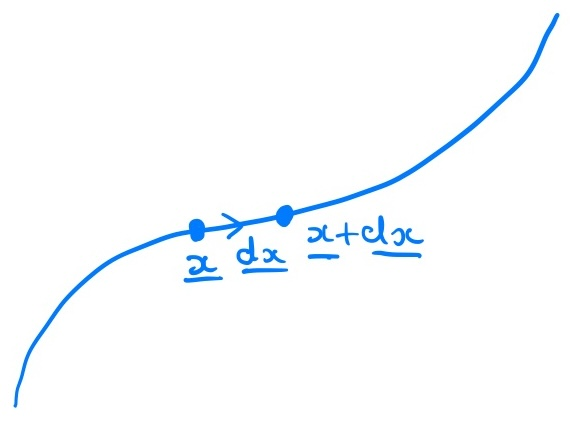
\includegraphics[width=\linewidth]{external/ch-chapter02-lagrange-problem2.jpg}
\end{image}%
\tcblower
\end{figureptx}%
\hyperref[lagrange-problem]{Figure~{\xreffont\ref{lagrange-problem}}} shows the points \(\bx(t)\) and \(\bx(t+dt)=\bx(t)+\de\bx\), and the equation for pathlines gives \(\de\bx=\bu(\bx,t)\de t\). We follow the value of \(f\) following a particle:%
\begin{align*}
\dd{f}{t}&=\lim_{\de t\rightarrow0}\frac1{\de t}\left(f(\bx+\de\bx,t+\de t)-f(\bx,t)\right)\\
&=\lim_{\de t\rightarrow0}\frac1{\de t}\left(f(\bx,t)+\de\bx\cdot\nabla f(\bx,t)+\de t\pd{f}{t}(\bx,t)+\dots-f(\bx,t)\right)\\
&=\lim_{\de t\rightarrow0}\frac1{\de t}\left(\bu(\bx,t)\de t\cdot\nabla f(\bx,t)+\de t\pd{f}{t}(\bx,t)+\dots\right)\\
&=\pd{f}{t}+\bu\cdot\nabla f=\DD{f}{t},
\end{align*}
('{}'{}\(\dots\)'{}'{} denotes higher order terms). Thus the value is preserved if \(\DD{f}{t}=0\).%
\item{}Show also that \(f\) is constant along streamlines if%
\begin{equation*}
\bu\cdot\nabla f=0.
\end{equation*}
%
\par\smallskip%
\noindent\textbf{\blocktitlefont Answer}.\hypertarget{ex-particle-paths-streamlines-4-2}{}\quad{}Now suppose that in \hyperref[lagrange-problem]{Figure~{\xreffont\ref{lagrange-problem}}}, we have shown instead the situation of a streamline.%
\par
In this case, the points \(\bx(s)\) and \(\bx(s+ds)=\bx(s)+\de\bx\) are shown, and the equation for streamlines gives \(\de\bx=\bu(\bx,t)\de s\). We follow the value of \(f\) along the streamline:%
\begin{align*}
\dd{f}{s}&=\lim_{\de s\rightarrow0}\frac1{\de s}\left(f(\bx+\de\bx,t)-f(\bx,t)\right)\\
&=\lim_{\de s\rightarrow0}\frac1{\de s}\left(f(\bx,t)+\de\bx\cdot\nabla f(\bx,t)-f(\bx,t)\right)\\
&=\lim_{\de s\rightarrow0}\frac1{\de s}\left(\bu(\bx,t)\de s\cdot\nabla f(\bx,t)\right)\\
&=\bu\cdot\nabla f.
\end{align*}
%
\par
Thus the value of \(f\) is preserved if \(\bu\cdot\nabla f=0\).%
\end{enumerate}%
\end{divisionexercise}%
\begin{divisionexercise}{6}{Streamlines, pathlines and streaklines.}{}{ex-streamlines-pathlines-streaklines}%
The velocity of a two-dimensional fluid flow in Cartesian coordinates is \(u = 1\), \(v = t e^{-4x}\). Calculate and sketch the following:%
\begin{enumerate}[font=\bfseries,label=(\alph*),ref=\alph*]%
\item{}the streamlines at a fixed time \(t > 0\),%
\par\smallskip%
\noindent\textbf{\blocktitlefont Answer}.\hypertarget{ex-streamlines-pathlines-streaklines-3-2}{}\quad{}The streamlines are given by%
\begin{equation*}
\pd{y}{x}=te^{-4x}\quad\Rightarrow\quad
y=y_0-\frac{t}{4} e^{-4x},
\end{equation*}
for any constant \(y_0\). Different values of \(y_0\) give different streamlines. See \hyperref[flowvisualisationproblem]{Figure~{\xreffont\ref{flowvisualisationproblem}}} for a sketch.%
\begin{figureptx}{Figure}{Sketch of streamlines, pathline and streaklines.}{flowvisualisationproblem}{}%
\begin{image}{0}{1}{0}{}%
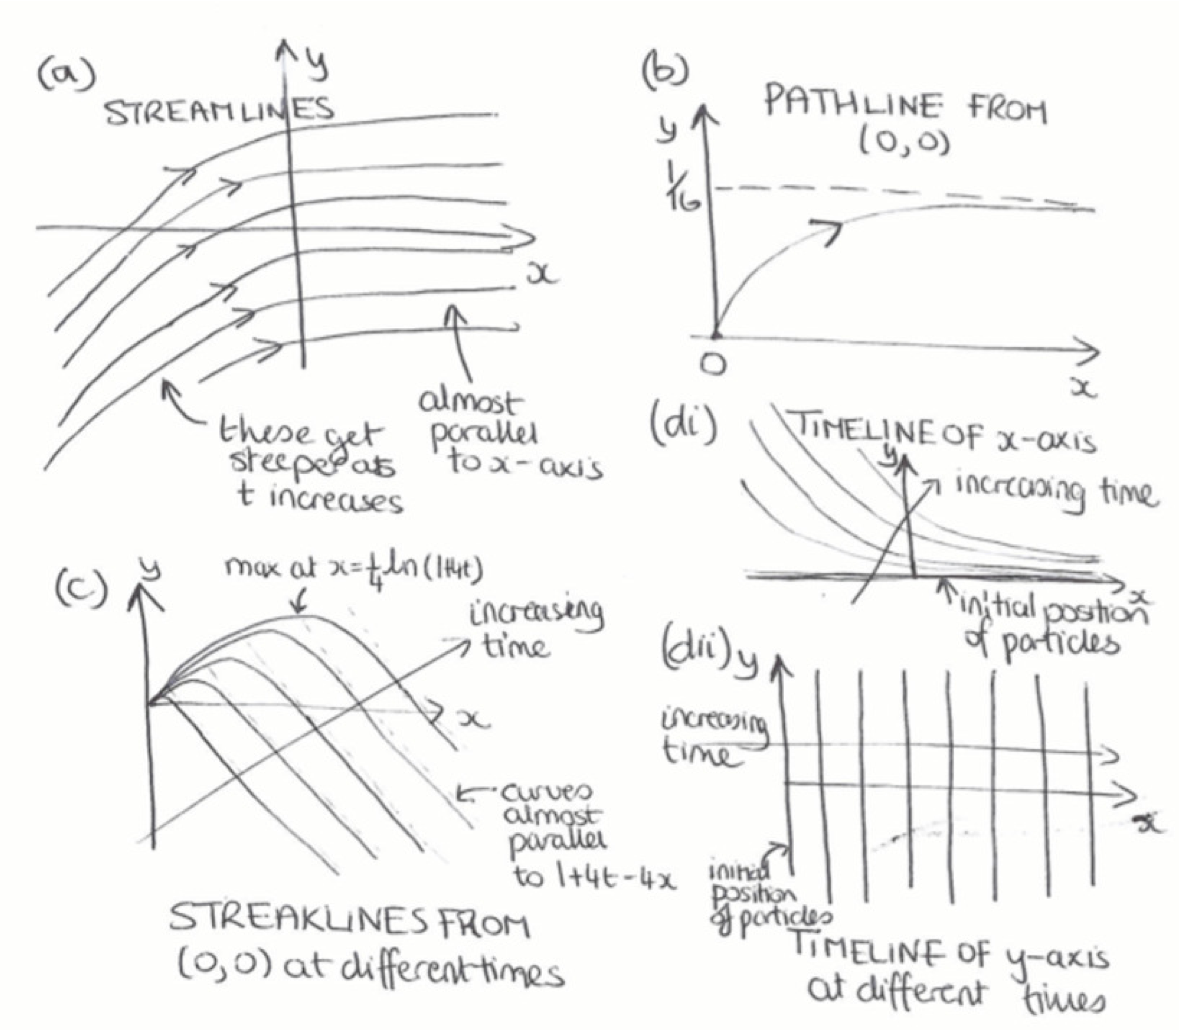
\includegraphics[width=\linewidth]{external/ch-chapter02-flowvisualisationproblem.png}
\end{image}%
\tcblower
\end{figureptx}%
\item{}the pathline of the particle starting from \((0,0)\),%
\par\smallskip%
\noindent\textbf{\blocktitlefont Answer}.\hypertarget{ex-streamlines-pathlines-streaklines-4-2}{}\quad{}The pathlines for a particle starting from \((x_0,y_0)\) are given by%
\begin{align*}
&\dd{x}{t}=1,\quad
\dd{y}{t}=te^{-4x}\\
\Rightarrow\quad&
x = x_0 + t,\quad
y = y_0 + \frac{1}{16} e^{-4x_0} - \frac{1+4t}{16} e^{-4(x_0+t)}.
\end{align*}
Eliminating \(t\):%
\begin{equation*}
y = y_0 + \frac{1}{16} e^{-4x_0}
- \frac{1+4x-4x_0}{16} e^{-4x}.
\end{equation*}
This is a general pathline. For the particular particle that starts from \((0,0)\):%
\begin{equation*}
y = \tfrac{1}{16}\left(1 - (1+4x)e^{-4x}\right).
\end{equation*}
See \hyperref[flowvisualisationproblem]{Figure~{\xreffont\ref{flowvisualisationproblem}}} for a sketch.%
\item{}and the streaklines passing through \((0,0)\).%
\par\smallskip%
\noindent\textbf{\blocktitlefont Answer}.\hypertarget{ex-streamlines-pathlines-streaklines-5-2}{}\quad{}Suppose the particle that started at \((x_0,y_0)\) hits the special point \((0,0)\) at time \(t_1\). From the pathline equation:%
\begin{equation*}
0 = x_0 + t_1, \quad
0 = y_0 + \tfrac{1}{16} e^{-4x_0}
- \tfrac{1+4t_1}{16} e^{-4(x_0+t_1)}.
\end{equation*}
Solving for \(x_0\) and \(y_0\):%
\begin{equation*}
x_0 = -t_1,\quad
y_0 = -\tfrac{1}{16}\left(e^{4t_1} - 1 - 4t_1\right).
\end{equation*}
At time \(t\) the particle is at:%
\begin{equation*}
x = t - t_1,\quad
y = \tfrac{1}{16}\left((1+4t_1) - (1+4t)e^{-4(t-t_1)}\right).
\end{equation*}
Eliminating \(t_1\) gives the streakline at time \(t\):%
\begin{equation*}
y = \tfrac{1}{16}\left((1+4t)(1-e^{-4x}) - 4x\right).
\end{equation*}
See \hyperref[flowvisualisationproblem]{Figure~{\xreffont\ref{flowvisualisationproblem}}} for a sketch. Note that the streamlines, pathlines and streaklines are all very different.%
\item{}For a line\slash{}curve in the \((x,y)\), its timeline at time \(t\) is the locus of the material elements at time \(t\) that started on the line\slash{}curve at \(t=0\). In experiments this can be visualised using a streak of dye placed initally along the line\slash{}curve. Tracking this over time gives the timelines.%
\par
Calculate and sketch the timelines of the line (i) \(y=0\), (ii) \(x=0\).%
\par\smallskip%
\noindent\textbf{\blocktitlefont Answer}.\hypertarget{ex-streamlines-pathlines-streaklines-6-2}{}\quad{}From the pathline equation, a particle starting from \((x_0,0)\) reaches%
\begin{equation*}
x = x_0 + t,\quad
y = \tfrac{1}{16} e^{-4x_0}
- \tfrac{1+4t}{16} e^{-4(x_0+t)}
\end{equation*}
at time \(t\). Eliminating \(x_0\) gives the timeline:%
\begin{equation*}
y = \tfrac{1}{16}\left(e^{4t} - 1 - 4t\right)e^{-4x}.
\end{equation*}
See \hyperref[flowvisualisationproblem]{Figure~{\xreffont\ref{flowvisualisationproblem}}} for a sketch.%
\par
From the pathline equation, a particle starting from \((0,y_0)\) reaches%
\begin{equation*}
x = t,\quad
y = y_0 + \tfrac{1}{16}
- \tfrac{1+4t}{16} e^{-4t}
\end{equation*}
at time \(t\). Since \(y_0\) can take any value, the timeline is just the line \(x = t\). See \hyperref[flowvisualisationproblem]{Figure~{\xreffont\ref{flowvisualisationproblem}}} for a sketch.%
\end{enumerate}%
\end{divisionexercise}%
\begin{divisionexercise}{7}{An experiment for the material derivative.}{}{ex-video-radioactive}%
\href{https://techtv.mit.edu/collections/ifluids/videos/32597-eulerian-and-lagrangian-descriptions-in-fluid-mechanics}{Watch around 12:00 to around 19:00 of the video "Eulerian and Lagrangian Descriptions of Fluid Mechanics" from the NCFMF archives}.%
\begin{enumerate}[font=\bfseries,label=(\alph*),ref=\alph*]%
\item{}In the video, the authors describe an experiment that one can setup to measure decay of a substance, say \(C(x, t)\) along a 1D segment in a river.%
\par
In the first situation, it is assumed that \(C\) is distributed uniformly in the river, but is a naturally decaying substance with some uniform rate of change, \(\dd{C}{t}\). Explain what is the (material) change in \(C\) that would be measured via two sensors, one upstream ane one downstream.%
\item{}Next, the authors imagine a situation where \(C\) is not uniformly distributed. They give a visual and analytical explanation of the material derivative,%
\begin{equation*}
\DD{C}{t} = \pd{C}{t} + u \pd{C}{x},
\end{equation*}
where \(u\) is the horizontal velocity within the infinitessimal 1D section. Write your own explanation of the above.%
\end{enumerate}%
\end{divisionexercise}%
\end{exercises-section}
\end{chapterptx}
%
%
\typeout{************************************************}
\typeout{Chapter 3 Equations of motion}
\typeout{************************************************}
%
\begin{chapterptx}{Chapter}{Equations of motion}{}{Equations of motion}{}{}{ch-chapter03-equations}
\renewcommand*{\chaptername}{Chapter}
\begin{introduction}{}%
In this chapter, we develop the basic equations of fluid dynamics. The equations are derived from applying principles of conservation of mass, momentum, and energy. In the simplest scenario, this leads to Euler's equation for a perfect (or ideal) fluid. Eventually, we relax these assumptions so as to incorporate the effects of viscosity.%
\par
Let \(D\) be a region in a 2D or 3D region filled with fluid. The fluid is in motion and we wish to describe this motion.%
\par
Let \(\bx\in D\) be a point in \(D\) and consider the particle of fluid that moves through the point \(\bx\) at time \(t\). In the figure below, we sketch the trajectory that this particle might take within the fluid. Also at the point \(\bx\) at time \(t\), we let \(\bu(\bx, t)\) be the velocity of the particle. At each fixed time, we can imagine the velocity vectors drawn at each point in the fluid; thus we call \(\bu\) the \emph{velocity field} of the fluid.%
\begin{figureptx}{Figure}{Image of the fluid domain \(D\).}{ch01-fluid}{}%
\begin{image}{0.25}{0.5}{0.25}{}%
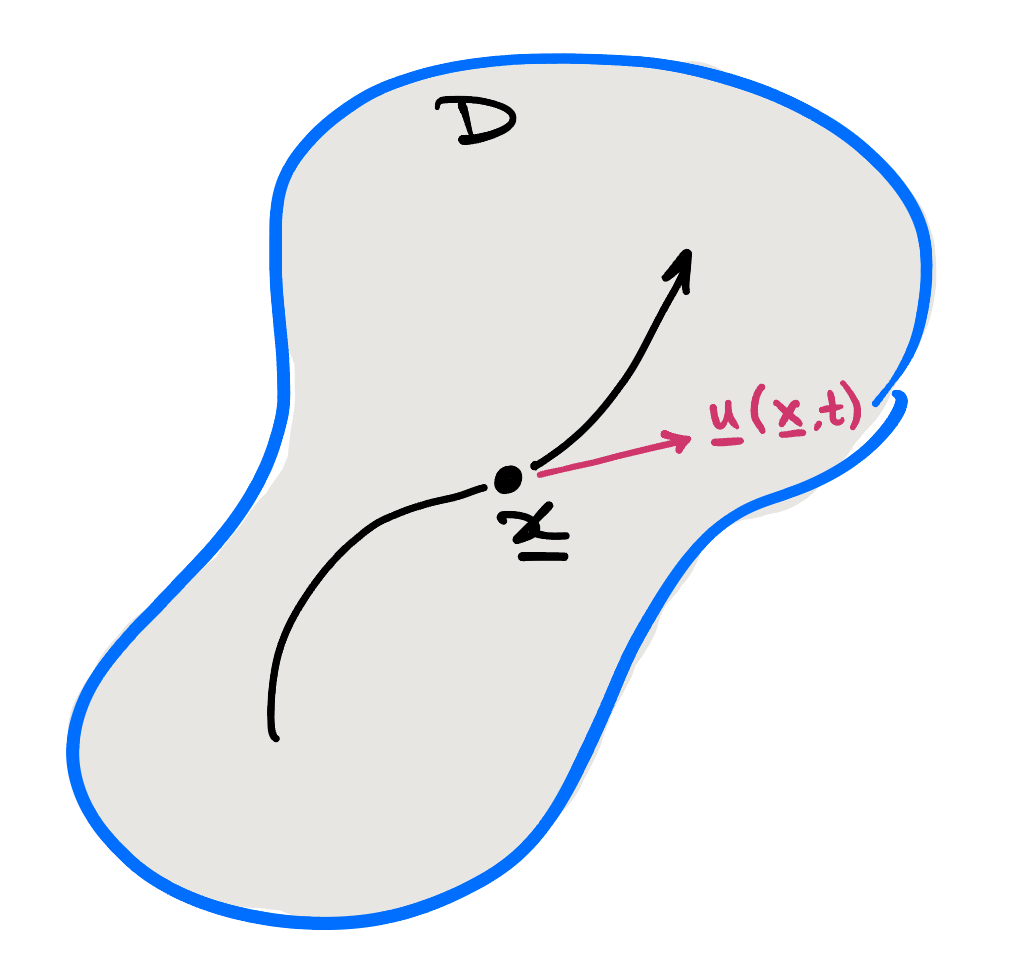
\includegraphics[width=\linewidth]{external/ch-chapter01-equations-fluid.png}
\end{image}%
\tcblower
\end{figureptx}%
At each point in space and moment in time, we assume that the fluid has a well-defined mass density, \(\rho(\bx, t)\). Let \(V \subseteq D\) be any subregion of \(D\). Then the mass of the fluid in \(V\) at time \(t\) is given by%
\begin{equation}
m(t) = \iiint_{V(t)} \rho(\bx, t) \, \mathrm{d}V.     \label{eqn-mass}
\end{equation}
%
\begin{remark}{Remark}{Smoothness and well-posedness.}{ch-chapter03-equations-2-6}%
In most of what follows in this chapter, we shall always assume that the functions \(\bu\), \(\rho\), and similarly for others describing fluid quantities are sufficiently smooth that the standard calculus operations can be applied to them. \emph{Can you think of some situations in fluid dynamics where smoothness might not be guaranteed?}%
\end{remark}
\begin{remark}{Remark}{Continuum assumption.}{rem-continuum}%
The assumption that the fluid can be described by a smooth scalar density field, \(\rho\), is a \emph{continuum assumption.} This is indeed one of the core assumptions that underlies this course, but it is worth noting that this is only an assumption (albeit a widely accepted one, applicable to most real-life scenarios). On the other extreme of this view is the assumption that the fluid is composed of a discrete set of molecules, all bouncing around, and hence fluid dynamics might be posed as the study of the kinetic motion of molecules!%
\par
In the continuum description, we are averaging properties (e.g. velocity) over groups of individual fluid particles that are close to each other. Thus there is a minimum size of the fluid body required for this approach to be valid (if we consider smaller sizes of fluid, the motion of individual particles becomes important):%
\begin{itemize}[label=\textbullet]
\item{}For gases at standard temperature and pressure (STP): the minimum volume is around \(10^{-18}\) m\(^3=1\) \(\mu\)m\(^3\) (this contains around \(3\times10^7\) molecules).%
\item{}For liquids: the minimum volume of fluid is smaller as the particles are closer together. For water, the minimum volume is around \(10^{-21}\) m\(^3\) (this contains around \(3\times10^7\) molecules).%
\item{}For complex fluids: the minimum volume needed to invoke the continuum approximation is often larger, e.g. blood contains red blood cells, which significantly affect its mechanics (the mechanics of blood plasma approximates that of water) and the volume of a single red blood cell is around \(10^{-16}\) m\(^3\).%
\end{itemize}
%
\end{remark}
In \hyperlink{ex-continuum-assumption}{Exercise~{\xreffont 3.6.1}}, you will consider whether salt flow can be considered under a continuum assumption.%
\begin{figureptx}{Figure}{An AI-generated image of salt flowing out of a large orifice.}{fig-salt-flow}{}%
\begin{image}{0.3}{0.4}{0.3}{}%
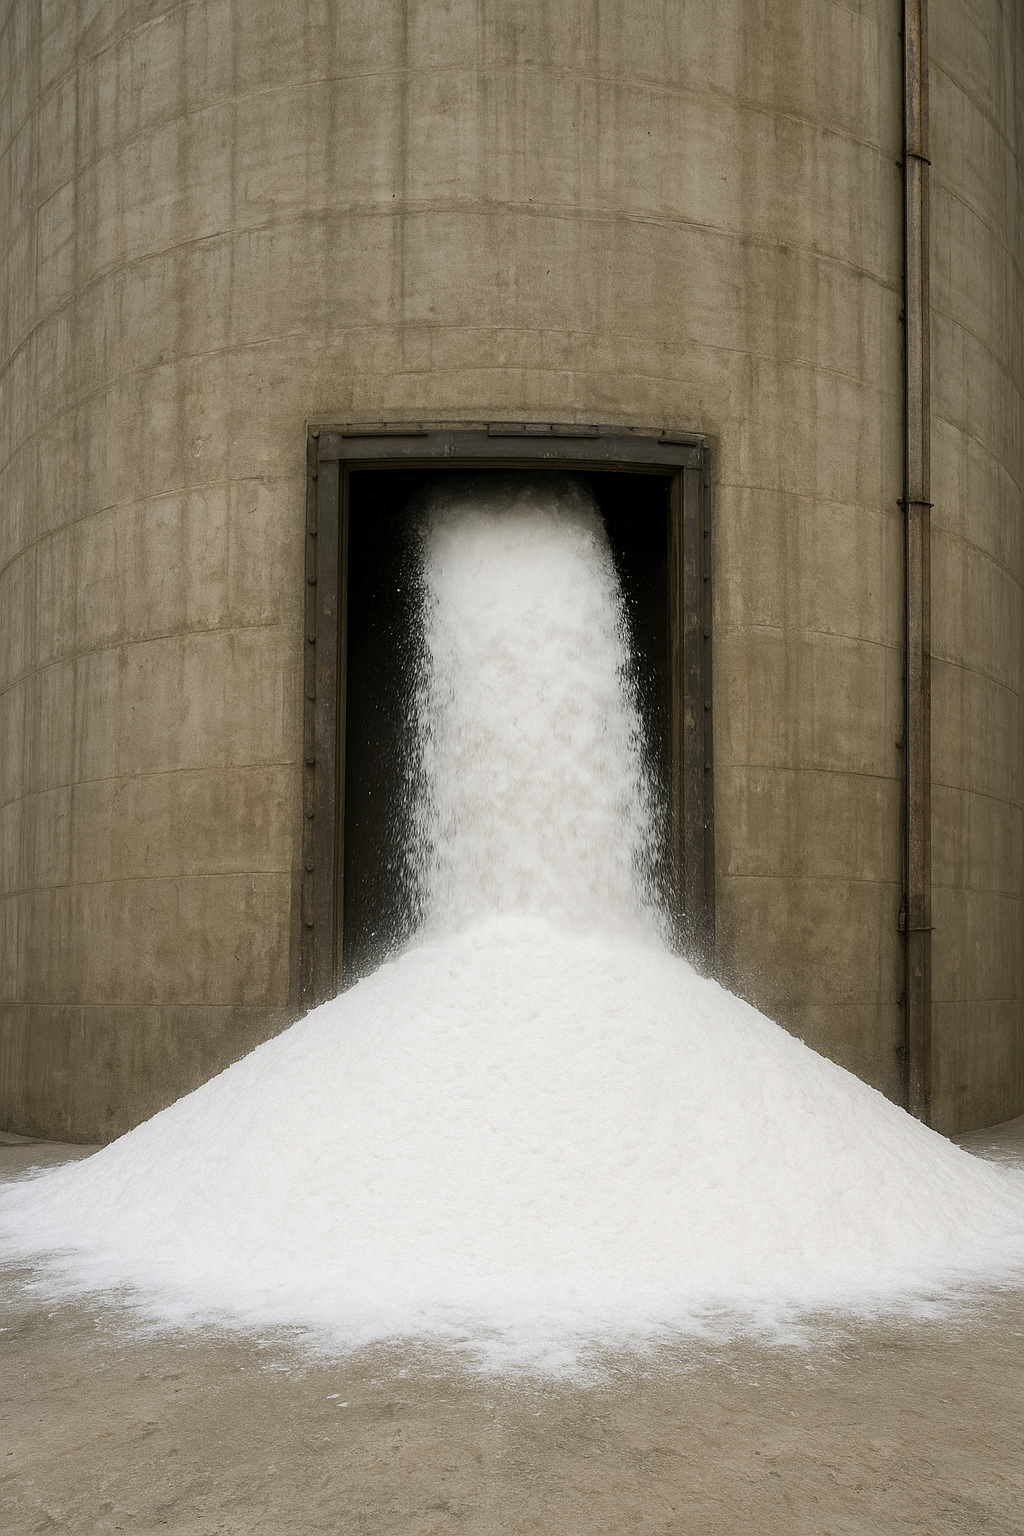
\includegraphics[width=\linewidth]{external/saltflow.png}
\end{image}%
\tcblower
\end{figureptx}%
The derivation of the governing equations for a fluid is then based on three basic principles of physics:%
\begin{enumerate}
\item{}\emph{Conservation of mass:} mass is neither created nor destroyed.%
\item{}\emph{Conservation of momentum:} the rate of change of momentum of a portion of the fluid is equal to the applied force (Newton's second law).%
\item{}\emph{Conservation of energy:} energy is neither created nor destroyed.%
\end{enumerate}
%
\par
Before starting, though, our first task is to derive some helpful results on the differentiation of quantities such as \hyperref[eqn-mass]{({\xreffont\ref{eqn-mass}})}.%
\end{introduction}%
%
%
\typeout{************************************************}
\typeout{Section 3.1 Reynolds' Transport Theorem}
\typeout{************************************************}
%
\begin{sectionptx}{Section}{Reynolds' Transport Theorem}{}{Reynolds' Transport Theorem}{}{}{sec-RTT}
%
%
\typeout{************************************************}
\typeout{Subsection 3.1.1 Jacobian of Lagrangian to Eulerian}
\typeout{************************************************}
%
\begin{subsectionptx}{Subsection}{Jacobian of Lagrangian to Eulerian}{}{Jacobian of Lagrangian to Eulerian}{}{}{subsec-jacob}
Consider a fluid volume, \(V \subset D\), that is initially dyed a certain colour. The packet of fluid is initially located at \(V(0)\). As the fluid evolves in time, it then occupies the volume \(V(t)\) with \(t > 0\).%
\par
As an example, we may express the density of the fluid as%
\begin{equation*}
\rho = \rho(\bx, t), \qquad \textrm{$\bx \in V(t)$}
\end{equation*}
i.e. at every point in space and moment in time, the above retrieves the density of the fluid within a designated region (which may be changing). This is a natural quantity to study in a fixed frame of the fluid.%
\par
Alternatively, we can write%
\begin{equation*}
\rho = \rho(\bX, t), \qquad \textrm{$\bX \in V(0)$}
\end{equation*}
which is the density of fluid for those particles making up an originally chosen volume, \(V(0)\). This is a natural quantity to study if we were to move with the fluid; for instance, if we were to colour the volume \(V(0)\) with a dye and track its density in time.%
\par
The correspondence between the Euclidean and Lagrangian coordinates is written as%
\begin{equation*}
\bx = \bx(\bX, t).
\end{equation*}
%
\begin{theorem}{Theorem}{Jacobian of Lagrangian to Eulerian.}{}{thm-jacobian}%
Since we assume the medium is continuous, then we would generally require that the mapping from Lagrangian to Eulerian coordinates is continuous and one-to-one; then the map assigns every element (label) in the original reference configuration, denoted \(\bX\), a unique position, \(\bx\), in the deformed state.%
\par
From Multivariable Calculus, a sufficient condition for this to be true is that the \emph{Jacobian of the transformation},%
\begin{equation*}
J = \pd{\bx}{\bX} = \pd{(x, y, z)}{(X, Y, Z)} =
\begin{vmatrix}
\pd{x}{X} & \pd{x}{Y} & \pd{x}{Z} \\
\pd{y}{X} & \pd{y}{Y} & \pd{y}{Z} \\
\pd{z}{X} & \pd{z}{Y} & \pd{z}{Z}
\end{vmatrix}
\end{equation*}
is finite and non-zero:%
\begin{equation*}
0 \lt J \lt \infty.
\end{equation*}
%
\end{theorem}
The following requires a bit of algebra, and you are not required to prove the result.%
\begin{theorem}{Theorem}{Euler's identity.}{}{thm-Euleridentity}%
The material derivative of the Jacobian of the transformation \(\bx = \bx(\bX, t)\) is given by%
\begin{equation}
\DD{J}{t} = J \nabla \cdot \bu,\label{eqn-euler-identity}
\end{equation}
where \(\bu =
\DD{\bx}{t}\).%
\end{theorem}
\begin{proof}{Proof}{}{thm-Euleridentity-3}
The proof follows from direct differentiation on the determinant and use of the identity of the material derivative.%
\end{proof}
\end{subsectionptx}
%
%
\typeout{************************************************}
\typeout{Subsection 3.1.2 Reynolds' Transport Theorem}
\typeout{************************************************}
%
\begin{subsectionptx}{Subsection}{Reynolds' Transport Theorem}{}{Reynolds' Transport Theorem}{}{}{subsec-RTT}
We are now ready to derive a key result that eases our path towards developing the governing equations for a fluid. The result is as follows.%
\begin{theorem}{Theorem}{Reynolds' Transport Theorem.}{}{thm-RTT}%
Consider a time-dependent volume, \(V(t)\), that is transported by the fluid so that it always consists of the same fluid particles. Then, for any function, \(f(\bx, t)\), continuously differentiable with respect to its arguments, \emph{Reynolds' Transport Theorem} is as follows:%
\begin{equation}
\dd{}{t} \iiint_{V(t)} f \, \de{x} \, \de{y} \, \de{z} = \iiint_{V(t)} \left[
\pd{f}{t} + \nabla \cdot (f\bu)\right] \, \de{x} \, \de{y} \, \de{z}.\label{eqn-RTT}
\end{equation}
%
\end{theorem}
\begin{proof}{Proof}{}{thm-RTT-3}
We transform the integral in Euclidean coordinates to Lagrangian coordinates, integrating in the label space:%
\begin{equation*}
I(t) \equiv \iiint_{V(t)} f \, \de{x} \de{y} \de{z}
= \iiint_{V(0)} f J \, \de{X} \de{Y} \de{Z},
\end{equation*}
and notice that we now only need to integrate over the fixed volume as defined in Lagrangian space, at the expense of adding the Jacobian factor. We now write%
\begin{align*}
\dd{I}{t} &= \iiint_{V(0)} \DD{(fJ)}{t} \, \de{X}\de{Y}\de{Z} 
\end{align*}
and the material derivative passes through since the domain is fixed. The \hyperref[thm-material-derivative]{Theorem~{\xreffont\ref{thm-material-derivative}}} now allows us to convert the material derivative to regular partial derivatives. By the chain rule:%
\begin{align*}
\DD{(fJ)}{t} &= \DD{f}{t}J + f\DD{J}{t} \\
&= \left[ \pd{f}{t} + \bu \cdot \nabla f\right]J
+ f \left[J \nabla \cdot \bu\right] \\
&= \left[ \pd{f}{t} + \nabla \cdot (f\bu) \right]J 
\end{align*}
and we have differentiated the Jacobian via Euler's identity \hyperref[thm-Euleridentity]{Theorem~{\xreffont\ref{thm-Euleridentity}}} in the second line. The last line follows from the chain rule applied to the vector identity:%
\begin{equation*}
\nabla \cdot (f\bu) = f \nabla \cdot \bu + \nabla f \cdot \bu.
\end{equation*}
We can now revert from Lagrangian to Eulerian integration, and this thus completes the proof of the Reynolds' Transport Theorem.%
\end{proof}
\begin{note}{Note}{}{subsec-RTT-4}%
It is helpful for you to convince yourself that the vector identity used in the proof is the only possible arrangement of operations that makes sense, i.e. in order for \(\nabla \cdot
(f\bu)\) to return a scalar.%
\end{note}
In summary: the Reynolds' Transport Theorem thus gives an identity for how time differentiation can pass through the integral when the domain of integration is changing in time!%
\begin{remark}{Remark}{A 1D version of the Reynolds' Transport Theorem.}{subsec-RTT-6}%
In 1D, Reynolds' Transport Theorem reduces to an identity known as Leibniz's rule. This is presented as an exercise in \hyperlink{ex-leibnitz-rule}{Exercise~{\xreffont 3.6.3}}.%
\end{remark}
\begin{remark}{Remark}{RTT and conserved quantities.}{subsec-RTT-7}%
Reynolds' Transport Theorem is particularly useful when the integral quantity%
\begin{equation*}
B = \iiint_{V(t)} f \, \de{x} \, \de{y} \, \de{z}
\end{equation*}
is a \emph{conserved quantity}. A conserved quantity is something for which we can apply a \emph{principle of conservation}. In practice for this course, this is usually mass or linear momentum:%
\begin{itemize}[label=\textbullet]
\item{}Mass: \(f=\rho\) and the left-hand side of \hyperref[eqn-RTT]{({\xreffont\ref{eqn-RTT}})} is zero because mass is conserved.%
\item{}Linear momentum: \(\bf=\rho\bu\) is now a vector quantity and, by \emph{Newton's second law}, the left-hand side of \hyperref[eqn-RTT]{({\xreffont\ref{eqn-RTT}})} equals the sum of the all the forces acting on the fluid in the control volume \(V\), which are:%
\begin{itemize}[label=$\circ$]
\item{}Surface forces: Forces acting on the surfaces of the fluid, which could be reaction forces from the walls of a container, or forces due to pressure or stress from surrounding fluid. (Note that we will cover stress in \hyperref[ch-viscousflows]{Chapter~{\xreffont\ref{ch-viscousflows}}}.)%
\item{}Body forces: Forces acting over the interior of the fluid, and in this course you will usually only need to consider the force of gravity, although in principle other body forces could act such as an electromagnetic force. In addition, if working in a noninertial frame of reference, other apparent forces need to be added (forces due to linear acceleration, angular acceleration and the Coriolis and centrifugal forces).%
\end{itemize}
%
\end{itemize}
%
\end{remark}
\begin{remark}{Remark}{General statement of RTT.}{rem-RTT-control-volume}%
\emph{Non-examinable:}%
\par
A more general statement of the Reynolds' Transport Theorem is as follows: We define a \emph{control volume} \(V(t)\). This is a region of the fluid that we specify; it could be any fluid-containing volume, and in particular it doesn't need to follow the fluid particles (unlike \hyperref[eqn-RTT]{({\xreffont\ref{eqn-RTT}})}). Then the rate of change of \(B\) in the system of particles equals the integral of the rate of change of \(f\) over the control volume plus the net flux of the \(f\) through the surface of the control volume:%
\begin{equation}
\dd{B_{\textrm{syst}}}{t} = \dd{B_{CV}}{t}+\dot{B}_{CS}.\label{eqn-RTT-simp}
\end{equation}
Here, \(B_{\textrm{syst}}\) is the amount of \(B\) in the system of particles, that is the Lagrangian derivative of \(B\), \(B_{CV}\) is the amount of \(B\) in the control volume and \(\dot{B}_{CS}\) is the flux of \(B\) across the surface of the control volume. Note that, if \(B\) is conserved then we can write the left-hand side in terms of other things (zero if \(B\) is mass and the sum of the forces if \(B\) is linear momentum).%
\par
This is in a form that can be used to solve many problems in engineering. The key point is that these problems are about quantities on the scale of the \emph{control volume} and not about the details of the flow at particular points.%
\par
Thus, for example we could consider a tank with inlets and outlets and, using the fluid in the tank as the control volume, we can apply the conservation of mass to find the volume flow rates in the inlets and outlets and the level of fluid in the tank.%
\par
We can use momentum conservation to find the force on a section of a pipe or the dynamics of a piston moving a fluid to which a known force is applied.%
\end{remark}
\end{subsectionptx}
\end{sectionptx}
%
%
\typeout{************************************************}
\typeout{Section 3.2 Conservation of mass}
\typeout{************************************************}
%
\begin{sectionptx}{Section}{Conservation of mass}{}{Conservation of mass}{}{}{ch-chapter03-equations-4}
\begin{introduction}{}%
Our task from this section is to prove the following equation for the conservation of mass of a fluid:%
\begin{theorem}{Theorem}{Continuity equation.}{}{thm-mass}%
The differential form of the law of conservation of mass, otherwise known as the \emph{continuity equation} is%
\begin{equation}
\pd{\rho}{t} + \nabla \cdot (\rho \bu) = 0,\label{eqn-consvmass1}
\end{equation}
where \(\rho = \rho(\bx,t)\) is the density of the fluid and \(\bu = \bu(\bx, t)\) is the velocity of the fluid.%
\par
The above form is equivalent, by the definition of the convective derivative, to%
\begin{equation}
\DD{\rho}{t} + \rho(\nabla \cdot \bu) = 0. \label{eqn-consvmass2}
\end{equation}
%
\end{theorem}
In fact, as it turns out, the proof of this result is trivial if we use the Reynolds' Transport Theorem and Lagrangian formulation following \hyperref[thm-RTT]{Theorem~{\xreffont\ref{thm-RTT}}}.%
\begin{proof}{Proof}{}{ch-chapter03-equations-4-2-4}
We consider the time differentiation of the mass integral,%
\begin{equation*}
\iiint_{V(t)} \rho \, \de{V},
\end{equation*}
for an arbitrary material volume \(V(t)\) in the fluid.%
\par
By \hyperref[thm-RTT]{Theorem~{\xreffont\ref{thm-RTT}}}, we can use the Reynolds' Transport Theorem to pass the time derivative through the integral. This gives:%
\begin{equation*}
\dd{}{t}\iiint_{V(t)} \rho \de{V} = \iiint_{V(t)} \left[ \pd{\rho}{t} + \nabla \cdot (\rho \bu)\right] \, \de{V},
\end{equation*}
which is satisfied for any volume \(V \subseteq D\) where the fluid is defined. Since the result is true for any such possible volume, then the integrand of the right hand-side, itself, must be zero. This gives immediately \hyperref[eqn-consvmass1]{({\xreffont\ref{eqn-consvmass1}})}.%
\par
The proof of \hyperref[eqn-consvmass2]{({\xreffont\ref{eqn-consvmass2}})} follows immediately from application of the definition of the convective derivative \hyperref[eqn-DDt]{({\xreffont\ref{eqn-DDt}})}.%
\end{proof}
Within the above proof, we use an idea used throughout this chapter, which is that if an integral of a quantity (the integrand) is zero for all possible domains of integration, then the integrand, itself, is zero. This is sometimes referred to as the "Bump lemma".%
\begin{lemma}{Lemma}{Bump lemma.}{}{lem-bump}%
Let \(f(\bx)\) be a sufficiently smooth function defined on \(\Omega \subseteq \mathbb{R}^n\). Suppose it is the case that%
\begin{equation*}
\int_V f(\bx) \, \de{V} = 0,
\end{equation*}
for all \(V \subseteq \Omega\). Then%
\begin{equation*}
f(\bx) \equiv 0
\end{equation*}
in \(\Omega\).%
\end{lemma}
In \hyperlink{ex-bump}{Exercise~{\xreffont 3.6.2}}, you will prove the above lemma.%
\end{introduction}%
%
%
\typeout{************************************************}
\typeout{Subsection 3.2.1 Derivation of mass conservation using Eulerian methods}
\typeout{************************************************}
%
\begin{subsectionptx}{Subsection}{Derivation of mass conservation using Eulerian methods}{}{Derivation of mass conservation using Eulerian methods}{}{}{ch-chapter03-equations-4-3}
The derivation we have just shown for \hyperref[thm-mass]{Theorem~{\xreffont\ref{thm-mass}}}, using the Lagrangian viewpoint and the Reynolds' Transport Theorem is misleadingly simple, and it can be instructive to see how the result is proved purely from the perspective of Eulerian coordinates.%
\par
For this, let us consider \(V\) to be a \emph{fixed and closed} subregion of the overall fluid, \(D\) that does not change with time. An illustration of this is shown in \hyperref[fig-normalvolume]{Figure~{\xreffont\ref{fig-normalvolume}}}.%
\begin{figureptx}{Figure}{Picture of the fluid volume, \(V\), shown in blue, with a small surface element, \(\partial V\), and the outwards flux.}{fig-normalvolume}{}%
\begin{image}{0.2}{0.6}{0.2}{}%
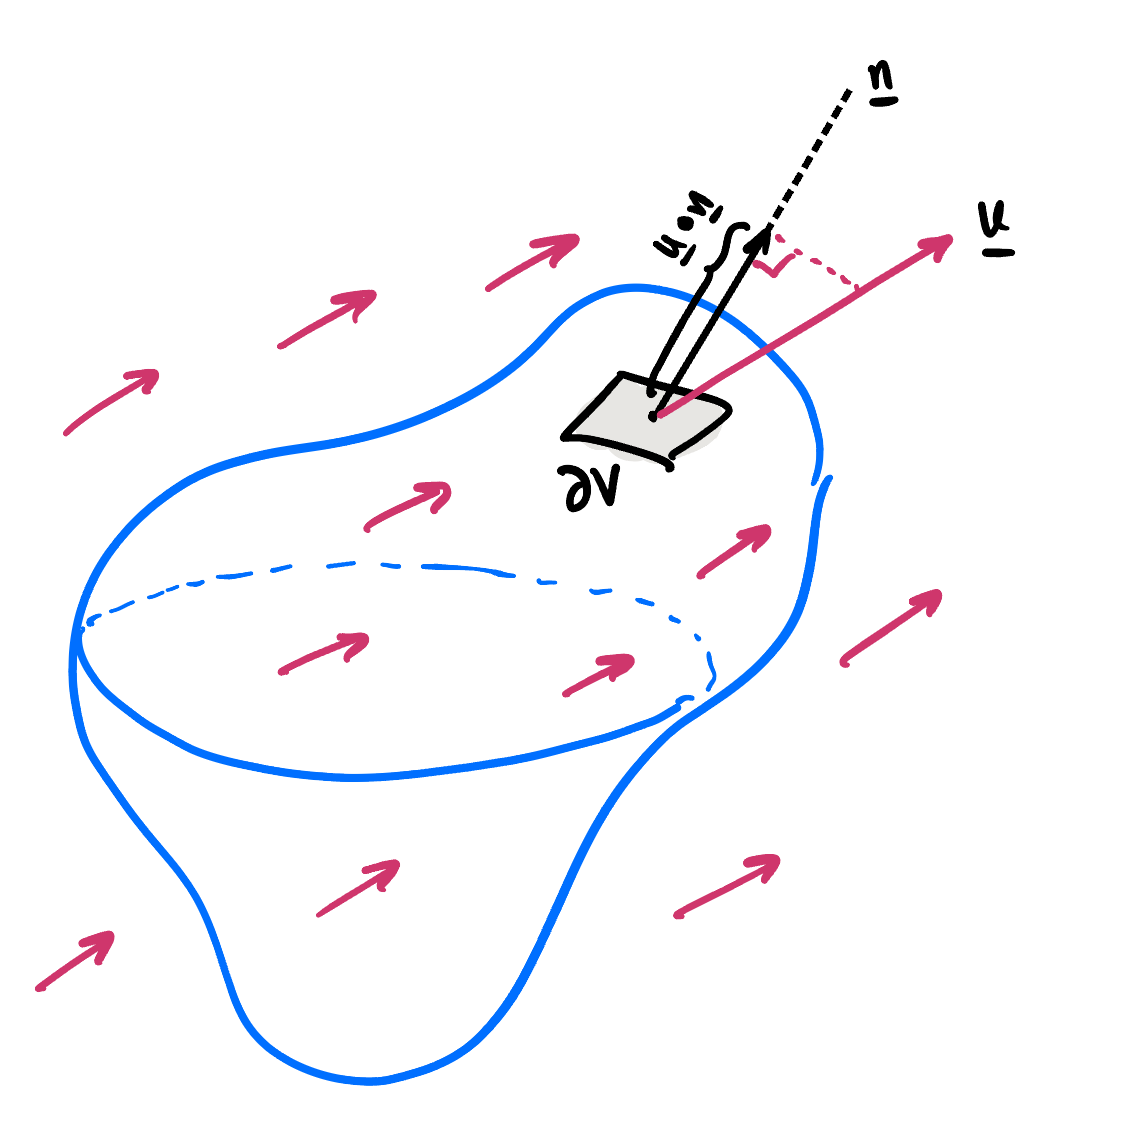
\includegraphics[width=\linewidth]{external/ch-chapter01-equations-09-54-13.png}
\end{image}%
\tcblower
\end{figureptx}%
We want to prove the following result, which essentially equates the change in mass, due to density changes, to the flow of mass in or out of the volume.%
\begin{theorem}{Theorem}{Integral form of the law of conservation of mass.}{}{ch-chapter03-equations-4-3-6}%
Given a fixed volume element \(V\) and boundary \(\partial V\), the integral form of the law of mass conservation is%
\begin{equation}
\dd{}{t} \iiint_V \rho \, \de{V} = -\iint_{\partial V} \rho \bu \cdot \bn \, \de{S}.\label{eqn-integralconservation}
\end{equation}
%
\end{theorem}
\begin{proof}{Proof}{}{ch-chapter03-equations-4-3-6-3}
The rate of change of mass in \(V\) is%
\begin{equation*}
\dd{}{t} \iiint_V \rho(\bx, t) \, \de V = \iiint_V \pd{\rho}{t} \, \de V,
\end{equation*}
and note the derivative passes through the integral since the volume, \(V\), does not change with time.%
\par
Let the boundary of \(V\) be given by \(\partial V\), and let \(\bn\) denote the outward unit normal defined along the boundary \(\partial V\). At each point on the boundary, the volume flow rate (known as the \emph{flux}) across the boundary is given by \(\bu
\cdot \bn\) and therefore the mass flow rate is \(\rho \bu \cdot \bn\).%
\par
We now sum the total mass flow across the entire boundary. This is given by the surface integral%
\begin{equation*}
\text{rate of mass change across $\partial V$} = \iint_{\partial V} \rho \bu \cdot \bn \,
\de{S}.
\end{equation*}
The flux out of the boundary is also sketched in \hyperref[fig-normalvolume]{Figure~{\xreffont\ref{fig-normalvolume}}}.%
\par
Mass conservation is now applied. Therefore, the rate of change of pass in the volume \(V\) is equal to the rate at which mass enters the boundary in the \emph{inwards} direction.%
\end{proof}
We now want to transform the integral form in \hyperref[eqn-integralconservation]{({\xreffont\ref{eqn-integralconservation}})} into the form of a partial differential equation. To do this, apply the \emph{Divergence theorem} to the right hand-side of the above integral, converting the surface integral to a volume integral. Moving all quantities to the left hand side now yields%
\begin{equation*}
\iiint_V \left[ \pd{\rho}{t} + \nabla \cdot (\rho \bu)\right] \, \de{V} = 0.
\end{equation*}
Since the above integral equation holds for all possible \(V\), it must be equivalent to the integrand equated to zero (\hyperref[lem-bump]{Lemma~{\xreffont\ref{lem-bump}}}). This yields our final result leading to \hyperref[thm-mass]{Theorem~{\xreffont\ref{thm-mass}}}.%
\end{subsectionptx}
%
%
\typeout{************************************************}
\typeout{Subsection 3.2.2 Corollary of the Transport Theorem}
\typeout{************************************************}
%
\begin{subsectionptx}{Subsection}{Corollary of the Transport Theorem}{}{Corollary of the Transport Theorem}{}{}{subsec-cor-consvmass}
\begin{corollary}{Corollary}{}{}{cor-convmass}%
There is a useful corollary to the transport theorem in \hyperref[thm-RTT]{Theorem~{\xreffont\ref{thm-RTT}}} in the case where the desired function of integration, \(f\), is proportional to the density, i.e. \(f = \rho h\) for any continuously differentiable \(h\). Indeed consider a moving volume \(V(t)\), and a density \(\rho\) that satisfies the continuity equation \hyperref[eqn-consvmass1]{({\xreffont\ref{eqn-consvmass1}})} or \hyperref[eqn-consvmass2]{({\xreffont\ref{eqn-consvmass2}})}. Then%
\begin{equation}
\dd{}{t} \iiint_{V(t)} \rho h \, \de{V} = \iiint_{V(t)} \rho \DD{h}{t} \, \de{V}.\label{eqn-cor-convmass}
\end{equation}
%
\end{corollary}
\begin{proof}{Proof}{}{cor-convmass-2}
This proof just follows from expansion. Pass the derivative through the integral and use the Reynolds' transport theorem formula. Then expand the quantity:%
\begin{equation*}
\nabla \cdot (f\bu) = \nabla f \cdot \bu + f \nabla \cdot \bu.
\end{equation*}
where \(f = \rho h\). Finally use the continuity equation on \(\rho\).%
\end{proof}
\end{subsectionptx}
\end{sectionptx}
%
%
\typeout{************************************************}
\typeout{Section 3.3 Momentum balance}
\typeout{************************************************}
%
\begin{sectionptx}{Section}{Momentum balance}{}{Momentum balance}{}{}{subsec-euler-momentum}
\begin{introduction}{}%
With mass conservation now handled, we turn our eyes towards a law that governs the conservation of momentum. This is \emph{Newton's second law} the rate of change of momentum of a body is equal to the sum of all forces acting on the body.%
\par
Our task from this section is to prove the following equation for the conservation of mass of a fluid:%
\begin{theorem}{Theorem}{Momentum equation.}{}{thm-momentum}%
The differential form of the law of conservation of momentum, is%
\begin{equation}
\rho \DD{\bu}{t} = \rho \left(\pd{\bu}{t} + \bu \cdot \nabla\bu\right) = - \nabla p + \rho \bg \label{eqn-consvmoment}
\end{equation}
where \(\rho = \rho(\bx,t)\) is the density of the fluid, \(\bu = \bu(\bx, t)\) is the velocity of the fluid, \(p = p(\bx, t)\) is the pressure, and \(\bg\) is the acceleration due to a body force (typically gravity).%
\end{theorem}
Note that above, we have used the notation \(\nabla \bu\) for the gradient of a vector. This is explained in \hyperref[remark-vector-gradient]{Remark~{\xreffont\ref{remark-vector-gradient}}}.%
\end{introduction}%
%
%
\typeout{************************************************}
\typeout{Subsection 3.3.1 Proof of the momentum equation for an inviscid fluid}
\typeout{************************************************}
%
\begin{subsectionptx}{Subsection}{Proof of the momentum equation for an inviscid fluid}{}{Proof of the momentum equation for an inviscid fluid}{}{}{subsec-euler-momentum-3}
Consider again a material volume \(V(t)\) of the fluid. Then the rate of change of net momentum of this volume is equal to%
\begin{equation}
\dd{}{t} \iiint_{V(t)} \rho \bu(\bx, t) \, \de{V}. \label{eqn-momentum1}
\end{equation}
It is helpful to remember that the mass of a volume element is \(\rho \de{V}\) and the acceleration is \(\dd{\bu}{t}\), so the above is similar to mass times acceleration. However, we work with the more general form above to allow for changes in the density throughout the fluid, and also for variable fluid elements, \(V(t)\).%
\par
We must equate the above to the sum of all surface and body forces applied to the fluid element.%
\par
An example of a body force is the force of gravity. For a small volume element of mass \(\rho \de{V}\), the force of gravity is equal to \((\rho \de{V})\bg\). Therefore, the total external force due to gravity on the volume is equal to%
\begin{equation}
\iiint_{V} \rho \bg \, \de{V}.\label{eqn-momentum2}
\end{equation}
There may be other external body forces. For example, if your fluid is electrically conductive (like a plasma), there may be electromagnetic forces that must be considered. In any case, \(\bg\) can be considered as the analogous body force.%
\par
The final type of forces we should consider are \emph{surface forces}, which are applied to the boundary of the fluid element, denoted \(\partial V\). Let us assume that at each point on the boundary, there is a per-surface area surface force, \(\bF\), that decomposes into component normal to the boundary, \(F_n \bn\), and a component tangential to the boundary, \(F_t \bt\). So the surface forces, summed over the boundary, will be%
\begin{equation}
\iint_{\partial V} \left[ F_n \bn + F_t \bt\right] \, \de{S}.\label{eqn-momentum-force}
\end{equation}
In the above, the interpretation is that the force on a small patch of surface area \(\de{S}\) is equal to the per-area force, say \(F_n\), multiplied by the area, then directed into the normal direction, \(\bn\).%
\par
At this point, we make a key assumption that is applied in the particular case of \emph{inviscid fluids}.%
\begin{theorem}{Theorem}{}{}{def-inviscid}%
In the case of \emph{inviscid fluids}, we assume that the surface pressure exerted on (interior) volume elements is accounted solely by a pressure, \(p\), which acts in the inward normal direction at each point, with \(F_n \bn = -p \bn\). Consequently, the surface force, given by \hyperref[eqn-momentum-force]{({\xreffont\ref{eqn-momentum-force}})}, is%
\begin{equation}
\iint_{\partial V} (-p) \bn \, \de{S} = \iiint_V (-\nabla p) \, \de{V}.\label{eqn-eqn-momentum-pressure}
\end{equation}
%
\par
In particular, for the case of inviscid fluids, we ignore tangential internal forces.%
\end{theorem}
\begin{proof}{Proof}{}{def-inviscid-2}
The result follows by a corollary of the diverence theorem. The divergence theorem is%
\begin{equation*}
\iiint_V \nabla \cdot \bF \, \de{V} = \iint_{\partial V} \bF \cdot \bn \, \de{S}.
\end{equation*}
Let \(\bF = p \boldsymbol{c}\) where \(\boldsymbol{c} = [1, 1, 1]\) and apply to the above.%
\end{proof}
Finally, it follows by summation of the forces above that Newton's law states that%
\begin{equation*}
\dd{}{t} \iiint_{V(t)} \rho \bu(\bx, t) \, \de{V} = -\iiint_V (\nabla p) \, \de{V} + \iiint \rho \bg \, \de{V}.
\end{equation*}
We can now use the corollary to the transport theorem \hyperref[cor-convmass]{Corollary~{\xreffont\ref{cor-convmass}}}, with the assignment of \(f = \rho u_x, \rho u_y, \rho u_z\) and this allows us to the conclude that%
\begin{equation*}
\iiint_{V} \left( \rho \DD{\bu}{t} + \nabla p - \rho \bg\right) \, \de{V} = 0.
\end{equation*}
Again, the above holds for all material volumes \(V\) and therefore it must follow that the integrand is zero. We conclude thus with the following result as stated in \hyperref[thm-momentum]{Theorem~{\xreffont\ref{thm-momentum}}}:%
\begin{equation*}
\rho \DD{\bu}{t} = - \nabla p + \rho \bg.
\end{equation*}
%
\par
In \hyperlink{ex-euler-check}{Exercise~{\xreffont 3.6.4}}, you will practice the derivation of the mass and momentum equations.%
\end{subsectionptx}
\end{sectionptx}
%
%
\typeout{************************************************}
\typeout{Section 3.4 The Euler equations}
\typeout{************************************************}
%
\begin{sectionptx}{Section}{The Euler equations}{}{The Euler equations}{}{}{sec-incompressible}
%
%
\typeout{************************************************}
\typeout{Subsection 3.4.1 Incompressible fluids and the Euler equations}
\typeout{************************************************}
%
\begin{subsectionptx}{Subsection}{Incompressible fluids and the Euler equations}{}{Incompressible fluids and the Euler equations}{}{}{sec-incompressible-2}
Recall from \hyperref[thm-Euleridentity]{Theorem~{\xreffont\ref{thm-Euleridentity}}} that the Jacobian relates infinitessimal volumes in Eulerian and Lagrangian frames via%
\begin{equation}
\dxyz = J \dXYZ\text{.}\label{eq-dxyz-Jacobian}
\end{equation}
So the Jacobian is a measure of the local expansion or contraction of a fluid (relative to its original state). If we use Euler's identity in the theorem, we are led to an important interpretation for what it means for a fluid to satisfy \(\nabla \cdot \bu = 0\). This leads us to defining the notion of an \emph{incompressible fluid.} (You already previously encountered an intuitive definition for an incompressible flow as part of \hyperlink{ex-video-flow-visualisation}{Exercise~{\xreffont 2.3.1}}).%
\begin{theorem}{Theorem}{Incompressible fluids.}{}{def-incompressible}%
A fluid is said to be \emph{incompressible} if it preserves infinitessimal volumes. Since such volumes are related via \hyperref[eq-dxyz-Jacobian]{({\xreffont\ref{eq-dxyz-Jacobian}})}, then this is equivalent to%
\begin{equation*}
\DD{J}{t} \equiv 0,
\end{equation*}
within the relevant fluid (and temporal) domain.%
\par
The following equivalence (iff) then follows:%
\begin{equation}
\textrm{Fluid is incompressible} \quad \Longleftrightarrow \quad \nabla \cdot \bu = 0.\label{eqn-incompressibledef}
\end{equation}
%
\end{theorem}
\begin{proof}{Proof}{}{def-incompressible-3}
Note that if \(\DD{J}{t} = 0\), then indeed the an infinitessimal volume element must be of static volume for all time according to \hyperref[eq-dxyz-Jacobian]{({\xreffont\ref{eq-dxyz-Jacobian}})}. Then by Euler's identity in \hyperref[thm-Euleridentity]{Theorem~{\xreffont\ref{thm-Euleridentity}}}, this implies \(\nabla \cdot \bu = 0.\) Conversely, if \(\nabla \cdot \bu = 0\), then again by the identity the fluid is incompressible.%
\end{proof}
So in conclusion, for the case of an incompressible fluid, it suffices to solve the equation%
\begin{equation}
\nabla \cdot \bu = 0,\label{eqn-divu}
\end{equation}
instead of the more complicated equation in \hyperref[thm-mass]{Theorem~{\xreffont\ref{thm-mass}}}.%
\par
By the way, what happens to the mass conservation equation in \hyperref[thm-mass]{Theorem~{\xreffont\ref{thm-mass}}} if the fluid is incompressible? This leads to the following corollary.%
\begin{corollary}{Corollary}{Constant density along streamlines.}{}{cor-incompressible-density}%
For an incompressible fluid, the density is constant along streamlines, i.e.%
\begin{equation*}
\DD{\rho}{t} = \pd{\rho}{t} + (\bu \cdot \nabla)\rho = 0.
\end{equation*}
%
\end{corollary}
\begin{proof}{Proof}{}{cor-incompressible-density-3}
This relies on setting \(\nabla \cdot \bu = 0\) in \hyperref[thm-mass]{Theorem~{\xreffont\ref{thm-mass}}}.%
\end{proof}
Let us return to consider the total sum of equations and unknowns. We have introduced the scalar mass conservation equation found in \hyperref[thm-mass]{Theorem~{\xreffont\ref{thm-mass}}} (or alternatively the more simplified equation \hyperref[eqn-divu]{({\xreffont\ref{eqn-divu}})} for incompressible fluids). Also the vector momentum equation found in \hyperref[thm-momentum]{Theorem~{\xreffont\ref{thm-momentum}}}. This yields four scalar equations for five unknowns: the pressure \(p\), density \(\rho\), and the three velocity components \(\bu\).%
\par
One way of proceeding is to attempt to establish or to inuit a relationship between pressure and density. For instance, the assumption of an ideal gas law can be derived from kinetic theory, which leads to the empirical law that \(p = RT\rho\), relating pressure in a linear fashion to density, and depending on the temperature, \(T\), and a (gas) constant \(R\). Other assumptions of the form \(p = p(\rho)\) are possible, and this is involved in the study of gases and \emph{compressible fluids}.%
\par
However, empirically, we observe that in most liquids, the density only varies within a few percent under typical variations of temperature and pressure. Therefore, it is common to assume:%
\begin{note}{Note}{Constant density assumption.}{sec-incompressible-2-10}%
We often assume that in the situation of liquids, the density is taken to be constant, \(\rho = \textrm{constant}\).%
\end{note}
Note, then that in the case of constant density fluids, if we consider the mass conservation equation \hyperref[eqn-consvmass1]{({\xreffont\ref{eqn-consvmass1}})}, it follows that \(\nabla \cdot \bu = 0\). Therefore, from the definition \hyperref[def-incompressible]{Theorem~{\xreffont\ref{def-incompressible}}}, we conclude that the fluid is indeed incompressible.%
\begin{remark}{Remark}{}{sec-incompressible-2-12}%
Confusingly, in many references, authors define a fluid to be incompressible if \(\rho\) is constant. However, we see this is not necessarily the case. A fluid can be incompressible and therefore \(\DD{\rho}{t} = 0\) without \(\rho\) being constant.%
\end{remark}
We are finally ready to state the \emph{Euler equations}.%
\begin{definition}{Definition}{Euler equations.}{def-euler}%
The \emph{Euler equations} consist of the continuity equation \hyperref[eqn-divu]{({\xreffont\ref{eqn-divu}})} and momentum equations \hyperref[eqn-consvmoment]{({\xreffont\ref{eqn-consvmoment}})}, considered in the situation of an incompressible fluid:%
\begin{align}
\nabla \cdot \bu &= 0, \label{def-euler-2-1-4-1}\\
\left(\pd{\bu}{t} + \bu \cdot \nabla\bu\right) &= - \frac{1}{\rho}\nabla p + \bg.\label{eqn-euler-momentum}
\end{align}
Note this is then four scalar equations for the three unknown velocities in \(\bu\) and pressure \(p\). We shall assume in the course that incompressible fluids have constant density, \(\rho\). The above Euler equations include the (gravitational) body force \(\bg\).%
\end{definition}
Simple applications of the Euler equations are given in \hyperlink{ex-kelvin-circulation-theorem}{Exercise~{\xreffont 6.3.1}}, \hyperlink{ex-fluid-pressure-uniform-velocity}{Exercise~{\xreffont 3.6.5}} and \hyperlink{ex-piston-fluid-problem}{Exercise~{\xreffont 3.6.6}}%
\par
You will consider the derivation of the Euler equations as part of \hyperlink{ex-euler-check}{Exercise~{\xreffont 3.6.4}}.%
\begin{example}{Example}{Computer graphics and fluid simulations.}{sec-incompressible-2-17}%
There has always been an intimate link between the research field of fluid mechanics and the entertainment field, where cutting-edge applications in animation, movie, and video-game graphics use ideas from fluid mechanics to model fluids. Many fluid simulators will use things like the Euler equations (or "bastardised version") to simulate fluids. In some cases, such simulations can even happen in real time. Here is an example of a real-time Euler equation solver \href{https://matthias-research.github.io/pages/tenMinutePhysics/17-fluidSim.html}{coded in Javascript.}%
\end{example}
\end{subsectionptx}
%
%
\typeout{************************************************}
\typeout{Subsection 3.4.2 Boundary conditions}
\typeout{************************************************}
%
\begin{subsectionptx}{Subsection}{Boundary conditions}{}{Boundary conditions}{}{}{subsec-euler-BCs}
\index{boundary conditions}%
A great deal of the complexity of fluid motion comes from the conditions that we must consider between the fluid and its bounding surfaces. For water in the ocean, a bounding surfaces might include the ocean floor bottom and the body of a boat, down to the vegetation in the water or the sand on a beach. \emph{This can get quite complex!} In this module, and when we first learn fluid dynamics, we only consider simple bounded fluid regions (fluid above a plate, fluid in a box, fluid in a channel, etc.)%
\par
In the case of a water wave, a bounding surface will also include the free surface of the wave, itself, which interacts with the surrounding atmospheric gas. This leads to the situation of free-boundary or free-surface conditions\index{free-surface}.%
\par
For the situation of fluid at a solid boundary, this leads us to formulate the following.%
\begin{note}{Note}{No-flux condition through a boundary.}{note-noflux-BC}%
For a fluid in contact with a fixed rigid boundary, \(\partial V\), then we require that the normal velocity of the fluid there must be zero:%
\begin{equation}
\bu \cdot \bn = 0 \quad \textrm{on $\partial V$},\label{eqn-motion-noflux-BC}
\end{equation}
where \(\bn\) is the unit normal to \(\partial V\). This condition states that the fluid cannot flow through \(\partial V\) or separate from \(\partial V\) (hence leaving a vacuum).%
\end{note}
It turns out that the above no-flux condition is sufficient to provide well-posed boundary conditions for most inviscid fluids. Note that in particular, we have not constrained the tangential velocity of the fluid, i.e. \(\bu \cdot \bt\), where \(\bt\) is the tangential vector at the boundary.%
\par
Later in \hyperref[ch-viscousflows]{Chapter~{\xreffont\ref{ch-viscousflows}}}, you will study the situation of a \emph{viscous fluid}, where it will be important to consider the tangential fluid velocity.%
\end{subsectionptx}
\end{sectionptx}
%
%
\typeout{************************************************}
\typeout{Section 3.5 Bernoulli's equation}
\typeout{************************************************}
%
\begin{sectionptx}{Section}{Bernoulli's equation}{}{Bernoulli's equation}{}{}{sec-bernoulli}
\begin{introduction}{}%
There is a reformulation of the momentum equations that proves to be useful. In essence, it emerges from attempting to integrate the momentum equation \hyperref[eqn-euler-momentum]{({\xreffont\ref{eqn-euler-momentum}})} and yields the famous \emph{Bernoulli equation(s)}.%
\par
We will first need a vector identity.%
\begin{identity}{Identity}{}{}{ident-ugradu}%
Note the following identity:%
\begin{equation}
(\bu \cdot \nabla) \bu = \nabla \left(\frac{1}{2}|\bu|^2\right) + (\nabla \times \bu) \times \bu. \label{eqn-ugradu}
\end{equation}
%
\end{identity}
\begin{proof}{Proof}{}{ident-ugradu-2}
The proof follows from direct expansion of both sides.%
\end{proof}
It will also be useful for us to introduce the notion of vorticity.%
\begin{definition}{Definition}{Vorticity of a vector field.}{def-vorticity}%
The \emph{vorticity}, \(\omega\), of a vector field is defined by%
\begin{equation}
\omega \equiv \nabla \times \bu.\label{eqn-vorticity}
\end{equation}
The vorticity is a measure of the local rotation of the flow.%
\end{definition}
Let us recall the definition of a \emph{conservative force}.%
\begin{definition}{Definition}{Conservative forces.}{def-conservative-force}%
A force \(\bF\) is a \emph{conservative force} if and only if there exists a potential \(\chi\), such that%
\begin{equation*}
\bF = -\nabla \chi,
\end{equation*}
in a simply connected region where the quantities are defined.%
\end{definition}
Note the distinction about a simply-connected neighbourhood. The above is not quite the definition of a conservative force (typically defined to be a force for which the work done on an object between two points is independent of path). For now, this is not an important distinction since we will focus on fluid regions that are free of holes. Until told otherwise, we will always assume that the fluid is simply connected and therefore the above serves as a definition of conservative forces.%
\begin{theorem}{Theorem}{Bernoulli's equation for steady flow.}{}{thm-bernoulli-steady}%
Bernoulli's equation (theorem) for steady flow states that%
\begin{equation}
B(\bx) \equiv \frac{p}{\rho} + \frac{1}{2} |\bu|^2 + \chi = \textrm{constant along streamlines},\label{eqn-bernoulli-steady}
\end{equation}
where we have assumed that the body force is \emph{conservative}, i.e. it can be written as%
\begin{equation}
\bg = -\nabla \chi, \label{eqn-gravity-potential}
\end{equation}
for a potential function, \(\chi\).%
\end{theorem}
\begin{proof}{Proof}{}{thm-bernoulli-steady-3}
Start from the momentum equation \hyperref[eqn-consvmoment]{({\xreffont\ref{eqn-consvmoment}})},%
\begin{equation*}
\pd{\bu}{t} + \bu \cdot \nabla\bu = - \frac{1}{\rho}\nabla p - \nabla \chi
\end{equation*}
and use the vector identity \hyperref[eqn-ugradu]{({\xreffont\ref{eqn-ugradu}})} gives%
\begin{equation*}
\pd{\bu}{t} + (\nabla \times \bu) \times \bu = - \nabla \left(\frac{1}{\rho}\nabla p + \frac{1}{2} |\bu|^2 + \chi\right).
\end{equation*}
%
\par
Next, the flow is steady, and therefore we can zero the first term. This leaves%
\begin{equation*}
\bomega \times \bu = -\nabla B.
\end{equation*}
We now take the dot product of both sides of the equation with \(\bu\). We use the fact that,%
\begin{equation*}
\bu \cdot (\bomega \times \bu ) = 0,
\end{equation*}
since it is a triple scalar product with two repeated entries. It therefore results in the fact that%
\begin{equation*}
\bu \cdot \nabla B = 0.
\end{equation*}
Notice that this is the steady component that comes from the material derivative, \(\DD{B}{t} = 0\). So we conclude that \(B\) is constant along streamlines of the flow.%
\par
It is useful to note that if we use the definition of vorticity in \hyperref[eqn-vorticity]{({\xreffont\ref{eqn-vorticity}})}, and the definition of \(B\) in \hyperref[eqn-bernoulli-steady]{({\xreffont\ref{eqn-bernoulli-steady}})}, we have from the above that%
\begin{equation}
\pd{\bu}{t} + \bomega \times \bu = -\nabla B,\label{eqn-bernoulli-vorticity}
\end{equation}
a form that will be useful, shortly.%
\end{proof}
\begin{remark}{Remark}{}{sec-bernoulli-2-10}%
For the typical gravity force directed in the \(-z\) direction, we can write \(\bg = -g[0, 0, 1] = -g \be_z\). So in this case, the (gravitational) potential is \(\chi = gz\).%
\end{remark}
The proof of \hyperref[thm-bernoulli-steady]{Theorem~{\xreffont\ref{thm-bernoulli-steady}}} introduced a useful form of the momentum equation using the vorticity function, resulting in \hyperref[eqn-bernoulli-vorticity]{({\xreffont\ref{eqn-bernoulli-vorticity}})}. This leads to the so-called \emph{vorticity equation} form of the momentum equation.%
\begin{theorem}{Theorem}{The vorticity equation for incompressible flow.}{}{thm-vorticity-equation}%
The momentum equation for incompressible flow, reposed in terms of the vorticity is:%
\begin{equation}
\pd{\bomega}{t} + (\bu \cdot \nabla)\bomega = (\bomega \cdot \nabla)\bu,\label{eqn-vorticity-equation}
\end{equation}
or, equivalently,%
\begin{equation}
\DD{\bomega}{t} = (\bomega \cdot \nabla)\bu,\label{eqn-vorticity-equation-lagrange}
\end{equation}
and is known as the \emph{vorticity equation}.%
\end{theorem}
In the proof, it is useful to use the vector identity for the curl of a cross product:%
\begin{equation}
\nabla \times (\bu \times \bv) = (\nabla \cdot \bv)\bu - (\nabla \cdot \bu)\bv + (\bv \cdot \nabla)\bu - (\bu \cdot \nabla)\bv.  \label{eqn-curlcross}
\end{equation}
%
\begin{proof}{Proof}{}{sec-bernoulli-2-14}
Crucially, we recall the result that "curl grad equals zero" for a vector field. So from \hyperref[eqn-bernoulli-vorticity]{({\xreffont\ref{eqn-bernoulli-vorticity}})}, we take the curl of both sides to obtain%
\begin{equation*}
\nabla \times \left(\pd{\bu}{t} + \bomega \times \bu\right) = 0.
\end{equation*}
Expanding the outer cross product, the first term can be simplified by swapping differentiation in space with differentiation in time. The second term requires the cross product identity \hyperref[eqn-curlcross]{({\xreffont\ref{eqn-curlcross}})}. For the second term, we get%
\begin{equation*}
-\nabla \times (\bu \times \bomega) = 0 - 0 + (\bomega \cdot \nabla)\bu - (\bu \cdot \nabla)\bomega,
\end{equation*}
with the first zero resulting in the fact that "div curl equals zero", while the second results from incompressibility.%
\par
Thus we have,%
\begin{equation*}
\pd{\bomega}{t} + (\bu \cdot \nabla)\bomega = (\bomega \cdot \nabla)\bu,
\end{equation*}
which is the main result.%
\end{proof}
You will prove this result from first principles in \hyperlink{ex-vorticity-equation}{Exercise~{\xreffont 3.6.7}}.%
\end{introduction}%
%
%
\typeout{************************************************}
\typeout{Subsection 3.5.1 Potential flow}
\typeout{************************************************}
%
\begin{subsectionptx}{Subsection}{Potential flow}{}{Potential flow}{}{}{subsec-potential}
We are interested in the simplest scenarios that will result in reducing the governing equations. Previosly, we introduced the notion of incompressible flows, which results in the Euler equations in \hyperref[def-euler]{Definition~{\xreffont\ref{def-euler}}} and in particular, the reduction of the mass conservation equation to \(\nabla \cdot \bu = 0\).%
\par
We attempt to reduce further by assuming that the fluid is \emph{irrotational}. This lends to the following definition.%
\begin{definition}{Definition}{Irrotational flows.}{def-irrotational}%
A flow is said to be \emph{irrotational} if the vorticity is identically zero:%
\begin{equation}
\textrm{flow is irrotational} \Longleftrightarrow  \bomega = \nabla \times \bu \equiv 0.\label{eqn-irrotational}
\end{equation}
%
\end{definition}
For an irrotational and incompressible flow, there is a more powerful version of Bernoulli's equation.%
\begin{theorem}{Theorem}{Bernoulli's equation for steady irrotational flow.}{}{thm-bernoulli-potential}%
For an incompressible and irrotational flow, Bernoulli's theorem states that%
\begin{equation}
B(\bx) \equiv \frac{p}{\rho} + \frac{1}{2} |\bu|^2 + \chi = \textrm{constant everywhere},\label{eqn-bernoulli-potential}
\end{equation}
where \(\bg = -\nabla \chi\) is the body force.%
\end{theorem}
\begin{proof}{Proof}{}{thm-bernoulli-potential-3}
The proof of this relies on returning to the proof of the unsteady Bernoulli's equation in \hyperref[thm-bernoulli-steady]{Theorem~{\xreffont\ref{thm-bernoulli-steady}}}. In the proof, we arrived at the result in \hyperref[eqn-bernoulli-steady]{({\xreffont\ref{eqn-bernoulli-steady}})} that%
\begin{equation*}
\pd{\bu}{t} + \bomega \times \bu = -\nabla B.
\end{equation*}
For steady flow, the first term disappears. If we have the additional assumption that the flow is irrotational, then we have that \(\bomega = 0\), and therefore we have%
\begin{equation*}
\nabla B = 0.
\end{equation*}
But the only way that all spatial derivatives is zero is if the function is constant.%
\end{proof}
You will practice an application of Bernoulli's equation in \hyperlink{ex-bernoulli-streamline}{Exercise~{\xreffont 3.6.8}}.%
\begin{example}{Example}{Airflow into or out of a room.}{subsec-potential-8}%
During the lecture, just for fun, we will play \href{https://www.youtube.com/watch?v=1L2ef1CP-yw}{this video by Matthias Wandel} about airflow out of a room. This is somewhat related to Bernoulli's equation (the connection between pressure and velocity), though the situation is considerably more difficult.%
\end{example}
\begin{example}{Example}{Pascal's bursting barrel.}{subsec-potential-9}%
For fun during the lecture, we will play \href{https://www.youtube.com/watch?v=EJHrr21UvY8}{this video demonstration done at Princeton} demonstrating the power of hydrostatic pressure.%
\end{example}
\begin{example}{Example}{Urination across species.}{subsec-potential-10}%
During the lecture, we will play \href{https://www.youtube.com/watch?v=EidLGwyYpBE}{this video describing} the work by Yang et al. on \href{https://www.pnas.org/doi/pdf/10.1073/pnas.1402289111}{"Duration of urination does not change with body size"}. The title is not quite accurate, and the article describe that for most mammals tested greater than about 3kg, this is true. Bernoulli's equation is used.%
\end{example}
\end{subsectionptx}
\end{sectionptx}
%
%
\typeout{************************************************}
\typeout{Exercises 3.6 Exercises}
\typeout{************************************************}
%
\begin{exercises-section}{Exercises}{Exercises}{}{Exercises}{}{}{ws-equations}
\begin{introduction}{}%
This chapter focused on deriving the key Euler equations for an inviscid and incompressible flow, starting from first principles, and deriving the conservation laws using vector calculus. Eventually, we studied different variations of the Euler equations and its consequences.%
\end{introduction}%
\begin{divisionexercise}{1}{Continuum approximation.}{}{ex-continuum-assumption}%
Domestic salt flows quite well out of a container with a hole in the bottom. Following \hyperref[rem-continuum]{Remark~{\xreffont\ref{rem-continuum}}}, consider whether salt matches up to the properties quoted for a fluid%
\par
What is the size of a typical salt particle? What size of hole would required so that a continuum model of the salt flow is a reasonable assumption? (Based on Q1, p. 42 by Paterson \hyperlink{ref-paterson}{[{\xreffont 10}]}.)%
\par\smallskip%
\noindent\textbf{\blocktitlefont Solution}.\hypertarget{ex-continuum-assumption-3}{}\quad{}Salt is not like a fluid because you can make it into a pile, whereas the surface of a resting fluid is always horizontal. However, some aspects of salt flow are similar to the flow of a fluid. A typical salt particle is approximately a cube of side \(0.5\) mm, and therefore has a volume of approximately \(10^{-10}\) m\(^3\). We need a size of hole that admits a very large number of particles. A reasonable value of the volume \(V\) appearing in the continuum approximation might be the volume of \(3\times10^7\) salt grains (this was the number of gas or liquid molecules quoted in the notes), i.e. \(3\times10^{-3}\) m\(^3\), which is a cube of side length approximately \(10\) cm. We need a hole that is many times this distance, perhaps a hole with a diameter of one metre or so might be reasonable!%
\end{divisionexercise}%
\begin{divisionexercise}{2}{Bump lemma.}{}{ex-bump}%
Within our derivations of the governing equations, we often make use of the so-called "Bump lemma" given in \hyperref[lem-bump]{Lemma~{\xreffont\ref{lem-bump}}}.%
\par
Give a proof of the lemma.%
\par\smallskip%
\noindent\textbf{\blocktitlefont Solution}.\hypertarget{ex-bump-3}{}\quad{}This proof assumes that the function \(f\) is not pathological (e.g. it cannot oscillate infinitely fast, take different values for rational vs. irrational, etc.). That's what we mean by "sufficiently smooth".%
\par
Assume that there exists a point \(\bx_0 \in \Omega\) where \(f(\bx_0) \neq 0\). Suppose without loss of generality \(f > 0\) here. Since \(f\) is sufficiently smooth (and in particular, it is continuous), then there exists a non-trivial neighbourhood near \(\bx_0\) where \(f > 0\) everywhere in this neighbourhood, say \(V_0\). Then \(\int_{V_0} f \, \de{V} = 0\), contradicting the assumption. Therefore \(f\) must be zero everywhere.%
\end{divisionexercise}%
\begin{divisionexercise}{3}{Leibnitz's rule.}{}{ex-leibnitz-rule}%
The Reynolds' Transport Theorem \hyperref[thm-RTT]{Theorem~{\xreffont\ref{thm-RTT}}}, which relates to the passage of a time derivative through an integral, is a general form of the 1D Leibnitz rule:%
\begin{align}
\dd{}{t} & \int_{a(t)}^{b(t)} f(x, t) \, \de{x} \notag\\
& = \int_{a(t)}^{b(t)} \pd{f}{t} \, \de{x} + f(b(t), t) \dot{b}(t) - f(a(t), t)\dot{a}(t).\label{eqn-leibnitz-rule}
\end{align}
%
\begin{enumerate}[font=\bfseries,label=(\alph*),ref=\alph*]%
\item{}Examine the figure in \hyperref[ex-fig-leibnitz]{Figure~{\xreffont\ref{ex-fig-leibnitz}}}. Can you associate the quantities in Leibnitz's rule with the circled elements in the figure?%
\begin{figureptx}{Figure}{Visual "proof" of Leibnitz's rule}{ex-fig-leibnitz}{}%
\begin{image}{0.05}{0.9}{0.05}{}%
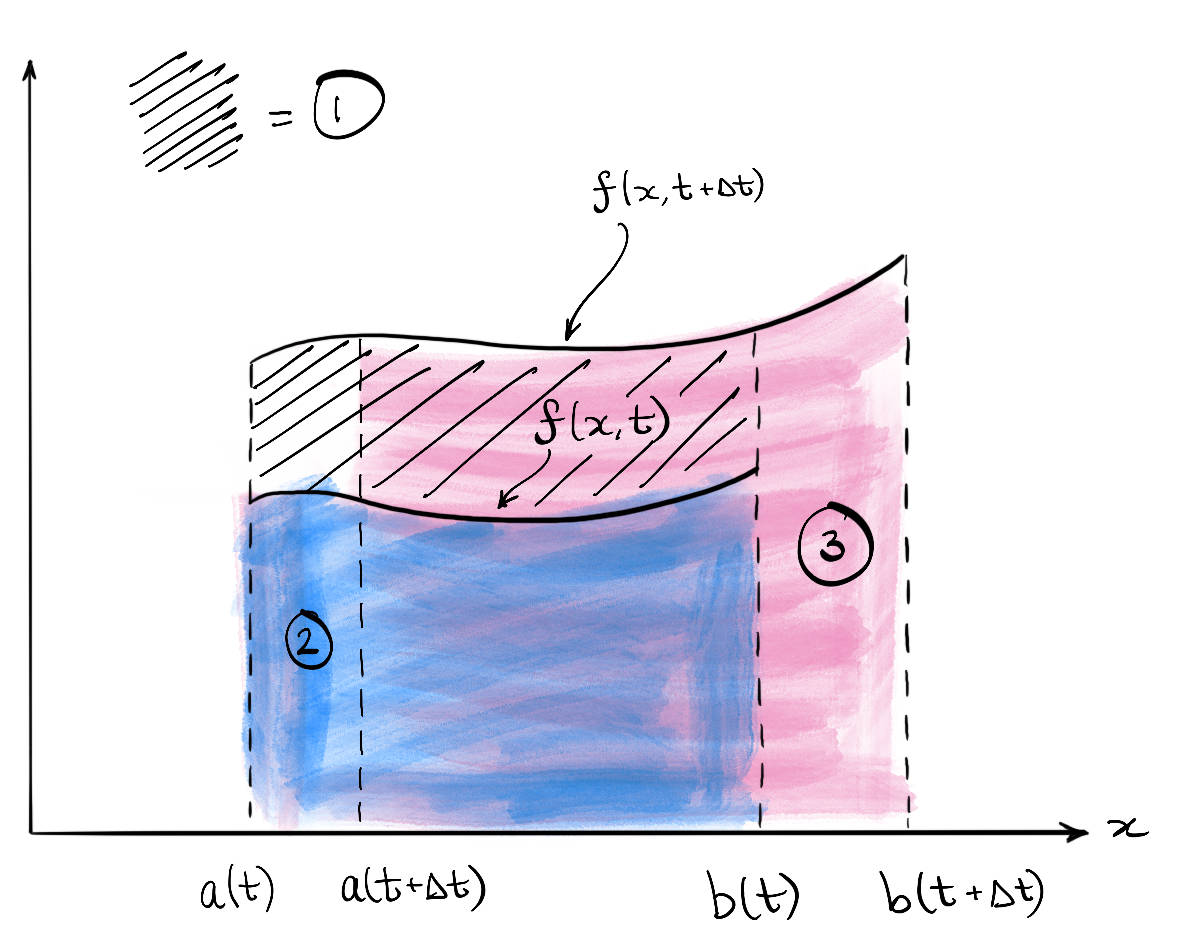
\includegraphics[width=\linewidth]{external/equations_leibnitz.jpg}
\end{image}%
\tcblower
\end{figureptx}%
\par\smallskip%
\noindent\textbf{\blocktitlefont Solution}.\hypertarget{ex-leibnitz-rule-3-2}{}\quad{}The first circled element is associated with the quantity:%
\begin{equation*}
\frac{1}{\Delta t} \int_{a(t)}^{b(t)} [f(x, t + \Delta t) - f(x, t)] \, \de{x}.
\end{equation*}
This is essentially the finite-difference version of the first term on the RHS.%
\par
The second circled element is associated with the quantity:%
\begin{equation*}
f(x, t)[a(t + \Delta t) - a(t)] \frac{1}{\Delta t},
\end{equation*}
and is associated with the area of the rectangle.%
\par
The third circled element is associated with%
\begin{equation*}
f(x, t + \Delta t)[b(t + \Delta t) - b(t)] \frac{1}{\Delta t},
\end{equation*}
and is associated with the area of the rectangle. Notice that for small \(\Delta t\), the rectangle height of \(f(x, t+\Delta t)\) is approximately the same as the rectangle height of \(f(x, t)\).%
\item{}A nice proof of the Leibnitz rule is given in \href{https://www.youtube.com/watch?v=zbWihK9ibhc}{this YouTube video by Brian Storey}. Watch the video and follow the derivation, making your own notes.%
\item{}Can you now connect the form of the rule in \hyperref[eqn-leibnitz-rule]{({\xreffont\ref{eqn-leibnitz-rule}})} to the Reynolds' Transport Theorem in \hyperref[eqn-RTT]{({\xreffont\ref{eqn-RTT}})}?%
\par\smallskip%
\noindent\textbf{\blocktitlefont Solution}.\hypertarget{ex-leibnitz-rule-5-2}{}\quad{}Write the second and third terms on the RHS as%
\begin{equation*}
\int_{a(t)}^{b(t)} \dd{}{x}(f(x, t) u(x, t)) \, \de{x}.
\end{equation*}
%
\end{enumerate}%
\end{divisionexercise}%
\begin{divisionexercise}{4}{Derivation of governing equations.}{}{ex-euler-check}%
\emph{This is a re-derivation of what is already presented in the notes, giving you valuable practice to understand the concepts.}%
\par
Starting from conservation of mass and momentum for a material volume moving in an inviscid fluid, use Reynolds' Transport Theorem \hyperref[eqn-RTT]{({\xreffont\ref{eqn-RTT}})} to derive the equations:%
\begin{gather}
\pd{\rho}{t} + \nabla \cdot(\rho \bu) = 0, \label{ex-euler-check-2-2-2-1}\\
\DD{\bu}{t} = -\frac{1}{\rho} \nabla p + \bg. \label{ex-euler-check-2-2-2-2}
\end{gather}
%
\par
What additional assumptions are required to transform the set of equations to the Euler equations of \hyperref[def-euler]{Definition~{\xreffont\ref{def-euler}}}? Apply these assumptions and conclude with the Euler equations.%
\par\smallskip%
\noindent\textbf{\blocktitlefont Solution}.\hypertarget{ex-euler-check-3}{}\quad{}The proof of the continuity equation is given in \hyperref[thm-mass]{Theorem~{\xreffont\ref{thm-mass}}} and the proof of the momentum equation is given in \hyperref[thm-momentum]{Theorem~{\xreffont\ref{thm-momentum}}}, so make sure you can follow these arguments and produce your own notes.%
\par
The derivation of the Euler equations, as given in \hyperref[def-euler]{Definition~{\xreffont\ref{def-euler}}} requires the additional assumption of an incompressible fluid, following \hyperref[def-incompressible]{Theorem~{\xreffont\ref{def-incompressible}}}. Incompressibility implies that \(\nabla \cdot \bu = 0\), and this equation then replaces the continuity equation.%
\end{divisionexercise}%
\begin{divisionexercise}{5}{Pressure field in uniform flow.}{}{ex-fluid-pressure-uniform-velocity}%
An ideal (incompressible and irrotational) fluid in a gravitational field with density \(\rho\) and acceleration vector \(\bg = -g \bk\) (with \(\bk\) being the unit vector in the positive \(z\)-direction) has uniform velocity%
\begin{equation*}
\bu = (a + b t, \; t^3, \; e^t).
\end{equation*}
The pressure at the origin is fixed at \(p_0\).%
\begin{enumerate}[font=\bfseries,label=(\alph*),ref=\alph*]%
\item{}Using the Euler equations in \hyperref[def-euler]{Definition~{\xreffont\ref{def-euler}}}, find the pressure field in terms of \(x, y, z, t, a, b, g, \rho\) and \(p_0\).%
\par\smallskip%
\noindent\textbf{\blocktitlefont Solution}.\hypertarget{ex-fluid-pressure-uniform-velocity-3-2}{}\quad{}The fluid has a uniform velocity, which means that all components of \(\nabla\bu\) vanish. The Euler equation simplifies to%
\begin{equation*}
\rho\pd{\bu}{t}=-\nabla p-\rho g \bk,
\end{equation*}
where%
\begin{equation*}
\pd{\bu}{t}=(b, \; 3t^2, \; e^t).
\end{equation*}
Hence, the pressure is given by solving the equation,%
\begin{equation*}
\nabla p = -\rho \pd{\bu}{t} - \rho g \bk
= -\rho (\, b, \; 3t^2, \; e^t + g \,),
\end{equation*}
which is a vector equation. Splitting into components, we obtain%
\begin{equation*}
\frac{\partial p}{\partial x} = -\rho b, \quad
\frac{\partial p}{\partial y} = -3\rho t^2, \quad
\frac{\partial p}{\partial z} = -\rho (e^t + g).
\end{equation*}
Solving sequentially, the first equation gives%
\begin{equation*}
p = -\rho b x + f_1(y,z,t).
\end{equation*}
Substituting into the second equation,%
\begin{equation*}
\frac{\partial f_1}{\partial y} = -3\rho t^2
\;\;\Rightarrow\;\;
f_1 = -3\rho t^2 y + f_2(z,t),
\end{equation*}
%
\begin{equation*}
p = -\rho b x - 3\rho t^2 y + f_2(z,t).
\end{equation*}
The third equation then implies%
\begin{equation*}
\frac{\partial f_2}{\partial z} = -\rho(e^t+g)
\;\;\Rightarrow\;\;
f_2 = -\rho(e^t+g)z + f_3(t),
\end{equation*}
%
\begin{equation*}
p = -\rho b x - 3\rho t^2 y - \rho(e^t+g)z + f_3(t).
\end{equation*}
Using \(p = p_0\) at the origin gives \(f_3(t) = p_0\) for all \(t\). Hence%
\begin{equation*}
p = p_0 - \rho \big(bx + 3t^2 y + (e^t + g)z \big).
\end{equation*}
%
\item{}Draw the contours of the pressure at a fixed time \(t\), and hence describe the pressure field.%
\par\smallskip%
\noindent\textbf{\blocktitlefont Solution}.\hypertarget{ex-fluid-pressure-uniform-velocity-4-2}{}\quad{}The pressure is constant on planes normal to the vector \((b, \; 3t^2, \; e^t + g)\), as illustrated below:%
\begin{figureptx}{Figure}{Contours of the pressure field at fixed \(t\).}{fig-pressure-contours}{}%
\begin{image}{0}{1}{0}{}%
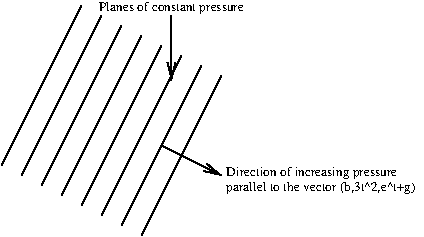
\includegraphics[width=\linewidth]{external/ch-chapter03-pressure-contours.png}
\end{image}%
\tcblower
\end{figureptx}%
\end{enumerate}%
\end{divisionexercise}%
\begin{divisionexercise}{6}{Piston problem.}{}{ex-piston-fluid-problem}%
The piston shown in the diagram below is pushed with a force \(F(t)\) into a pipe of length \(L\) and cross-sectional area \(A\) containing incompressible and irrotational fluid of density \(\rho\).%
\begin{figureptx}{Figure}{Schematic of piston and pipe system.}{fig-piston}{}%
\begin{image}{0}{1}{0}{}%
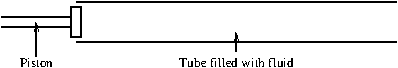
\includegraphics[width=\linewidth]{external/ch-chapter03-piston.png}
\end{image}%
\tcblower
\end{figureptx}%
Assume that the pressure at the open end is held at atmospheric pressure, \(p = p_\text{atm}\).%
\par
Assume the fluid moves as a rigid body and neglect friction and the mass of the piston. Using the Euler equations in \hyperref[def-euler]{Definition~{\xreffont\ref{def-euler}}}, write down a differential equation governing the position, \(X(t)\), of the piston at time \(t\). You may neglect gravity.%
\par\smallskip%
\noindent\textbf{\blocktitlefont Solution}.\hypertarget{ex-piston-fluid-problem-3}{}\quad{}We assume that the fluid pressure at the open end of the pipe is atmospheric pressure. Since the fluid moves as a rigid body, the velocity field has no spatial gradients, and hence the Euler equation reduces to%
\begin{equation*}
\rho\pd{\bu}{t}=-\nabla p,
\end{equation*}
where the velocity is uniformly \(\bu = (\dot{X}(t), 0)\).%
\par
Solving for \(p\) and using the fact that \(p\) is atmospheric pressure at \(x = L\), we have%
\begin{equation*}
p(x,t) = \rho\dd{^2 X}{t^2}(L-x)+p_\text{atm}.
\end{equation*}
%
\par
At the piston side, the pressure is equal to%
\begin{equation*}
\frac{F}{A} + p_\text{atm},
\end{equation*}
(recall pressure is force per unit area, therefore the piston force must be divided by \(A\)). Then%
\begin{equation*}
\frac{F+Ap_{atm}}{A} = \rho\dd{^2X}{t^2}(L-X)+p_{atm}
\quad\Rightarrow\quad
\dd{^2X}{t^2} = \frac{F}{A\rho(L-X)}.
\end{equation*}
%
\end{divisionexercise}%
\begin{divisionexercise}{7}{The vorticity equation.}{}{ex-vorticity-equation}%
Consider an incompressible fluid, with constant density \(\rho\), subject to a conservative body force (i.e. \({\bg} = -\nabla \chi\) for some potential function \(\chi\)).%
\begin{enumerate}[font=\bfseries,label=(\alph*),ref=\alph*]%
\item{}Starting from the Euler equations, show that the vorticity \(\bomega = \nabla \times {\bu}\) satisfies%
\begin{equation*}
\frac{D \bomega}{Dt} = (\bomega \cdot \nabla){\bu}.
\end{equation*}
Note that, in this question, you are expected to do a long-form calculation. The method given in the notes uses an alternative expression for the momentum equation combined with a vector identity to get the same result with less effort.%
\par\smallskip%
\noindent\textbf{\blocktitlefont Solution}.\hypertarget{ex-vorticity-equation-3-2}{}\quad{}The Euler equation reads:%
\begin{equation*}
\rho\left(\pd{\bu}{t} + (\bu \cdot \nabla)\bu\right) = -\nabla p - \rho\nabla \chi.
\end{equation*}
Since the curl of a gradient is zero, \(\rho\) is constant and we can commute derivatives, taking the curl of both sides gives%
\begin{equation*}
\rho\left(\pd{\bomega}{t} + \nabla \times(\bu \cdot \nabla)\bu\right) = 0.
\end{equation*}
We have%
\begin{align*}
& \nabla \times(\bu \cdot \nabla)\bu,\\
=&\begin{vmatrix}
\bi & \bj & \bk \\
\pd{}{x} & \pd{}{y} & \pd{}{z} \\
\bu \cdot \nabla u & \bu \cdot \nabla v & \bu \cdot \nabla w
\end{vmatrix},\\
=&\bi\left(\bu\cdot\nabla\left(\pd{w}{y}-\pd{v}{z}\right)+\pd{\bu}{y}\cdot\nabla w-\pd{\bu}{z}\cdot\nabla v\right)\\
&+\bj\left(\bu\cdot\nabla\left(\pd{u}{z}-\pd{w}{x}\right)+\pd{\bu}{z}\cdot\nabla u-\pd{\bu}{x}\cdot\nabla w\right)\\
&+\bk\left(\bu\cdot\nabla\left(\pd{v}{x}-\pd{u}{y}\right)+\pd{\bu}{x}\cdot\nabla v-\pd{\bu}{y}\cdot\nabla u\right),\\
=&\bu\cdot\nabla\bomega-\bomega\cdot\nabla\bu+\bomega\cdot\nabla\bu\\
&+\bi\left(\pd{u}{y}\pd{w}{x}+\pd{v}{y}\pd{w}{y}+\pd{w}{y}\pd{w}{z}-\pd{u}{z}\pd{v}{x}-\pd{v}{z}\pd{v}{y}-\pd{w}{z}\pd{v}{z}\right)\\
&+\bj\left(\pd{u}{z}\pd{u}{x}+\pd{v}{z}\pd{u}{y}+\pd{w}{z}\pd{u}{z}-\pd{u}{x}\pd{w}{x}-\pd{v}{x}\pd{w}{y}-\pd{w}{x}\pd{w}{z}\right)\\
&+\bk\left(\pd{u}{x}\pd{v}{x}+\pd{v}{x}\pd{v}{y}+\pd{w}{x}\pd{v}{z}-\pd{u}{y}\pd{u}{x}-\pd{v}{y}\pd{u}{y}-\pd{w}{y}\pd{u}{z}\right),\\
=&\bu\cdot\nabla\bomega-\bomega\cdot\nabla\bu\\
&+\bi\left(\left(\pd{w}{y}-\pd{v}{z}\right)\pd{u}{x}+\left(\pd{u}{z}-\pd{w}{x}\right)\pd{u}{y}+\left(\pd{v}{x}-\pd{u}{y}\right)\pd{u}{z}\right)\\
&+\bj\left(\left(\pd{w}{y}-\pd{v}{z}\right)\pd{v}{x}+\left(\pd{u}{z}-\pd{w}{x}\right)\pd{v}{y}+\left(\pd{v}{x}-\pd{u}{y}\right)\pd{v}{z}\right)\\
&+\bk\left(\left(\pd{w}{y}-\pd{v}{z}\right)\pd{w}{x}+\left(\pd{u}{z}-\pd{w}{x}\right)\pd{w}{y}+\left(\pd{v}{x}-\pd{u}{y}\right)\pd{w}{z}\right)\\
&+\bi\left(\pd{u}{y}\pd{w}{x}+\pd{v}{y}\pd{w}{y}+\pd{w}{y}\pd{w}{z}-\pd{u}{z}\pd{v}{x}-\pd{v}{z}\pd{v}{y}-\pd{w}{z}\pd{v}{z}\right)\\
&+\bj\left(\pd{u}{z}\pd{u}{x}+\pd{v}{z}\pd{u}{y}+\pd{w}{z}\pd{u}{z}-\pd{u}{x}\pd{w}{x}-\pd{v}{x}\pd{w}{y}-\pd{w}{x}\pd{w}{z}\right)\\
&+\bk\left(\pd{u}{x}\pd{v}{x}+\pd{v}{x}\pd{v}{y}+\pd{w}{x}\pd{v}{z}-\pd{u}{y}\pd{u}{x}-\pd{v}{y}\pd{u}{y}-\pd{w}{y}\pd{u}{z}\right),\\
=&\bu\cdot\nabla\bomega-\bomega\cdot\nabla\bu+\bomega\nabla\cdot\bu,\\
=&\bu\cdot\nabla\bomega-\bomega\cdot\nabla\bu,
\end{align*}
where the final equality follows from incompressibility. Hence,%
\begin{equation*}
\pd{\bomega}{t} + \bu\cdot\nabla\bomega - \bomega\cdot\nabla\bu = 0
\quad\Rightarrow\quad
\DD{\bomega}{t} = (\bomega \cdot \nabla)\bu,
\end{equation*}
as required.%
\item{}Deduce that, in two-dimensional incompressible flow, \(\omega\) is conserved following the flow.%
\par\smallskip%
\noindent\textbf{\blocktitlefont Solution}.\hypertarget{ex-vorticity-equation-4-2}{}\quad{}If the flow is the \((x,y)\)-plane, we have \(w=0\) and all \(z\)-derivatives are zero. Hence the only non-zero component of the vorticity is the \(z\)-component, \(\omega_z=\partial v/\partial x-\partial u/\partial y\). Thus%
\begin{equation*}
\bomega\cdot\nabla\bu=\omega_z\pd{\bu}{z}=0.
\end{equation*}
Hence%
\begin{equation*}
\DD{\bomega}{t} = 0,
\end{equation*}
meaning that \(\bomega\) is conserved following the flow.%
\end{enumerate}%
\end{divisionexercise}%
\begin{divisionexercise}{8}{Using streamlines: The clepsydra.}{}{ex-bernoulli-streamline}%
One of the earliest means for measuring the passage of time, invented by the ancient Egyptians, was the \terminology{clepsydra} (or ‘water thief’): a large jar with a hole in its base is filled with water. The shape of the jar was such that the interval of time taken for the water surface to pass two equally-spaced markers on the side of the jar is constant.%
 \begin{figureptx}{Figure}{Clepsyndra}{fig-clepsydra}{}%
\begin{image}{0.25}{0.5}{0.25}{}%
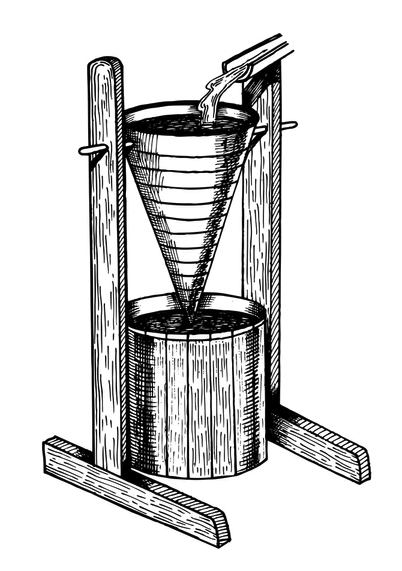
\includegraphics[width=\linewidth]{external/clepsydra.png}
\end{image}%
\tcblower
\end{figureptx}%
 In this question you will determine the shape of jar required to achieve this. In particular, we denote the (axisymmetric) jar radius a height \(z\) above the hole by \(r = a(z)\). The radius of the hole, \(a_h \ne a(0)\), in general.%
\begin{enumerate}[font=\bfseries,label=(\alph*),ref=\alph*]%
\item{}Explain why the curve \(r = a(z)\) is a streamline.%
\par\smallskip%
\noindent\textbf{\blocktitlefont Solution}.\hypertarget{ex-bernoulli-streamline-3-2}{}\quad{}The fluid velocity at the surface of the jar satisfies \(\bu\cdot\bn=0\), so that no fluid leaves or enters the jar through its sides. Thus,%
\begin{equation*}
\bu \cdot \bn = u_r - u_z \pd{a}{z} = 0.
\end{equation*}
This is precisely the condition for \(r = a(z)\) to be a streamline.%
\item{}If the surface of the water lies at \(z = h(t)\), use an appropriate form of Bernoulli’s principle to calculate the speed of liquid, \(u\), leaving the jar at \(z = 0\).%
\par
[You may assume that the desired surface speed \(u_S = |\dot{h}| \ll u\), so that the flow is approximately steady and that the fluid pressure is atmospheric at \(z = 0\).]%
\par\smallskip%
\noindent\textbf{\blocktitlefont Solution}.\hypertarget{ex-bernoulli-streamline-4-2}{}\quad{}We apply Bernoulli's equation to equate the energy at a point at the edge of the free surface at \(z = h(t)\) and the fluid leaving the hole at \(z = 0\). At the free surface, the pressure is atmospheric, \(p = p_{atm}\), and the speed is \(u_S\sqrt{1+a^{'2}}\). At the hole, the pressure is also atmospheric, \(p = p_{atm}\), and the velocity is \(u\). Thus, Bernoulli's equation for the streamline joining the two points gives%
\begin{equation*}
\frac{p_{atm}}{\rho} + \frac12 u_S^2(1+a^{'2}) + gh = \frac{p_{atm}}{\rho} + \frac12 u^2.
\end{equation*}
Assuming that \(u_S \ll u\), this simplifies to%
\begin{equation*}
gh = \frac12 u^2.
\end{equation*}
%
\item{}Use the principle of conservation of mass to link \(u_S\), \(u\), \(a_h\) and \(a(h(t))\); thereby determine the correct shape for a clepsydra.%
\par\smallskip%
\noindent\textbf{\blocktitlefont Solution}.\hypertarget{ex-bernoulli-streamline-5-2}{}\quad{}The volume flux out of the hole is \(\pi a_h^2 u\), while the rate of decrease of the volume of fluid in the jar is \(\pi a(h(t))^2 u_S\). Conservation of mass therefore gives%
\begin{equation*}
\pi a^2 u_S = \pi a_h^2 u,
\end{equation*}
or%
\begin{equation*}
u_S = \frac{a_h^2}{a^2}u.
\end{equation*}
Using the result from part (b) to eliminate \(u\) gives%
\begin{equation*}
u_S = \frac{a_h^2}{a^2}\sqrt{2gh}.
\end{equation*}
We require \(u_S\) to be independent of time so that equally spaced intervals are traversed in equal times. Hence,%
\begin{equation*}
a=\left(\frac{a_h^2\sqrt{2g}}{u_S}\right)^{1/2} h^{1/4}.
\end{equation*}
The terms in the brackets are constant, so we have that the radius of the jar must vary as the fourth root of the height.%
\end{enumerate}%
\end{divisionexercise}%
\end{exercises-section}
\end{chapterptx}
%
%
\typeout{************************************************}
\typeout{Chapter 4 Potential flows}
\typeout{************************************************}
%
\begin{chapterptx}{Chapter}{Potential flows}{}{Potential flows}{}{}{ch-chapter04-potentialflows}
\renewcommand*{\chaptername}{Chapter}
\begin{introduction}{}%
Typically, the most basic introduction on fluid dynamics usually involves the study of two-dimensional incompressible and irrotational flows, otherwise known as \emph{potential flows}. There is a good reason for this: the theory is elegant, visualisable, and uses to its benefit the enormous power of complex-variable theory.%
\par
Previously, we defined the concept of vorticity via \(\omega = \nabla \times \bu\), which serves as a measure of the local angular velocity of the flow. It turns out that in 2D, irrotational flows, with \(\omega = 0\), provide a powerful restricton to the complexity of flows, allowing the development of the above \emph{potential flow theory.}.%
\begin{figureptx}{Figure}{From "Fundamental Principles of Flows" and "Characteristics of the Laminar and Turbulent Flows" by Hunter Rouse. Courtesy of IIHR, University of Iowa.}{ch-chapter04-potentialflows-2-3}{}%
\begin{sidebyside}{2}{0.075}{0.075}{0.17}%
\begin{sbspanel}{0.47}%
\noindent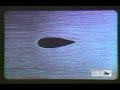
\includegraphics[width=\linewidth]{generated/youtube/ch-chapter04-potentialflows-2-3-2.jpg}
\end{sbspanel}%
\begin{sbspanel}{0.21}%
\noindent
\includegraphics[width=\linewidth]{generated/qrcode/ch-chapter04-potentialflows-2-3-2.png}
\href{https://trinh.github.io/BathMAFluids/ch-chapter04-potentialflows-2-3-2.html}{Standalone}%
\end{sbspanel}%
\end{sidebyside}%
\tcblower
\end{figureptx}%
\end{introduction}%
%
%
\typeout{************************************************}
\typeout{Section 4.1 The velocity potential}
\typeout{************************************************}
%
\begin{sectionptx}{Section}{The velocity potential}{}{The velocity potential}{}{}{sec-Potential-and-streamfunction}
\begin{introduction}{}%
In this chapter, we focus on 2D flows where the velocity vector is given by%
\begin{equation*}
\bu(x, y, t) = u(x, y, t)\bi + v(x, y, z)\bj = [u, v].
\end{equation*}
With the velocity given as above, the vorticity is then%
\begin{equation}
\bomega = \nabla \times \bu = \left(\pd{v}{x} - \pd{u}{y}\right)\bk.\label{eqn-2d-vorticity}
\end{equation}
If we assume that the flow is irrotational according to \hyperref[def-irrotational]{Definition~{\xreffont\ref{def-irrotational}}}, then \(\nabla \times \bu = 0\) and%
\begin{equation}
\pd{v}{x} - \pd{u}{y} = 0.\label{eqn-2d-irrotational}
\end{equation}
%
\par
Further, we know that if the flow is irrotational, then there exists a \emph{velocity potential}, \(\phi\), such that \(\bu = \nabla \phi\). Thus the velocities are expressed as%
\begin{equation}
u = \pd{\phi}{x} \quad \textrm{and} \quad v = \pd{\phi}{y}.\label{eqn-vel-potential}
\end{equation}
%
\par
The above result about irrotational flows is a standard result in Vector Calculus, but we will re-state the result here for reference, and provide a review of its proof.%
\begin{theorem}{Theorem}{Existence of a potential.}{}{thm-exist-potential}%
Consider a three-dimensional time-dependent velocity field, \(\bu = \bu(\bx, t)\) defined on a simply connected domain \(\bx\in D \subset \mathbb{R}^3 \times \mathbb{R}^+.\)%
\par
Then \(\bu\) is irrotational, i.e. \(\nabla \times \bu = 0\) if and only if there exists a scalar potential, defined on \(D \times \mathbb{R}^+\), such that \(\bu = \nabla \phi\).%
\end{theorem}
\begin{proof}{Proof}{}{thm-exist-potential-3}
Define%
\begin{equation*}
\phi(\bx, t) \equiv \phi_0(t) + \int_C \bu \cdot \de{x},
\end{equation*}
where \(C\) is any contour connecting an arbitrary origin point to the point \(\bx\) (changing the origin point will change the "constant" of integration \(\phi_0(t)\)).%
\par
We can verify, using the definition of differentiation, and the fundamental theorme of calculus, applied along each of the three coordinate directions, that \(\nabla \phi = \bu\) as desired.%
\par
The key is to prove that the above definition is unique, regardless of the choice of contour \(C\). To this end, consider two contours, \(C_1\) and \(C_2\), both with the same origin point, \(O\), and end point \(P\). Then the contour \(C_1 - C_2\) is a close contour beginning and ending at \(O\).%
\begin{figureptx}{Figure}{Proof of the uniqueness of the potential}{fig-potential-proof}{}%
\begin{image}{0.1}{0.8}{0.1}{}%
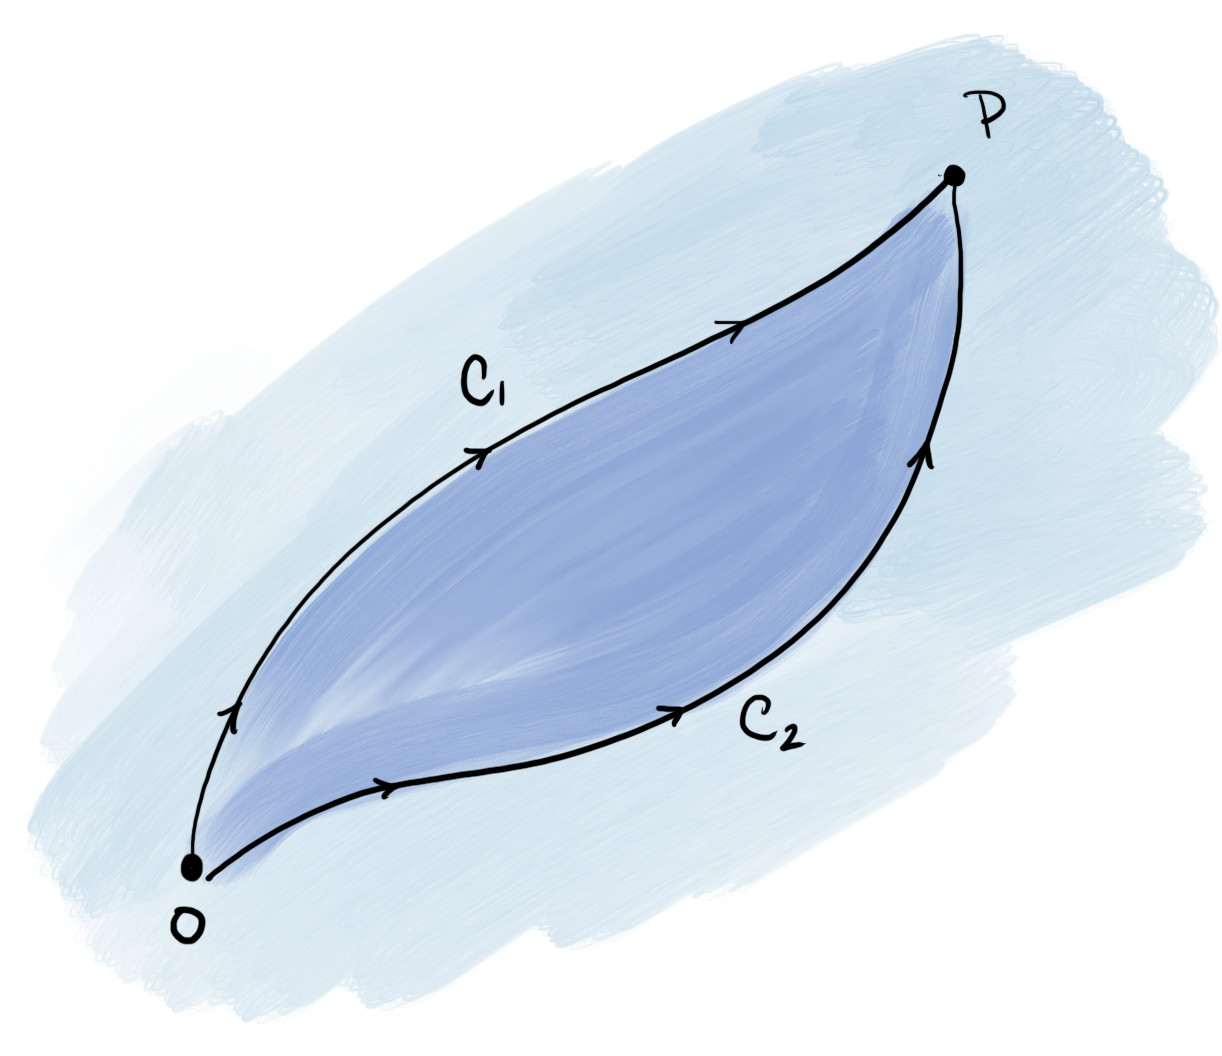
\includegraphics[width=\linewidth]{external/potentialproof.jpg}
\end{image}%
\tcblower
\end{figureptx}%
By Stokes' theorem,%
\begin{equation*}
\int_{C_1 - C_2} \bu \cdot \de{x} = \iint_S (\nabla \times \bu) \, \bn \, \de{S}, 
\end{equation*}
where \(S\) is any surface with bounding curve \(C_1 - C_2\), and with unit normal \(\bn\) positively oriented with the bounding curve. However, the right hand-side is zero by irrotationality, and therefore%
\begin{equation*}
\int_{C_1} \bu \cdot \de{x} = \int_{C_2} \bu \cdot \de{x},
\end{equation*}
and our choice of curve in the definition of the potential is irrelevant.%
\par
The converse direction of the theorem follows directly from the fact that "curl grad equals zero", i.e. \(\nabla \times \nabla \phi = 0\).%
\end{proof}
Let us return to discussing the setting of potential flow.%
\par
In addition to being irrotational, we furthermore have assumed that the flow is incompressible. Therefore from \hyperref[def-incompressible]{Theorem~{\xreffont\ref{def-incompressible}}},%
\begin{equation}
\nabla \cdot \bu = \pd{u}{x} + \pd{v}{y} = \pd{^2\phi}{x^2} + \pd{^2\phi}{y^2} = 0.\label{eqn-2d-divu}
\end{equation}
This is the crucial result, which is that in potential flows, we need only solve the Laplace equation:%
\begin{equation}
\nabla^2 \phi = 0,\label{eqn-2d-laplace}
\end{equation}
within the flow region. This is effectively a single linear equation for the single unknown \(\phi\). However, for different problems, the boundary conditions can render even this "simple" problem difficult.%
\par
Once the velocity potential \(\phi\) has been solved, the velocities in the flow can be recovered from the relationship \hyperref[eqn-vel-potential]{({\xreffont\ref{eqn-vel-potential}})}. The pressure in the flow also follows from Bernoulli's equation. For the situation of a steady potential flow, following \hyperref[thm-bernoulli-potential]{Theorem~{\xreffont\ref{thm-bernoulli-potential}}}, it is%
\begin{equation}
\frac{p}{\rho} + \frac{1}{2} |\nabla \phi|^2 + \chi = \textrm{constant}.\label{eqn-2d-bernoulli}
\end{equation}
%
\end{introduction}%
%
%
\typeout{************************************************}
\typeout{Subsection 4.1.1 Elementary flows}
\typeout{************************************************}
%
\begin{subsectionptx}{Subsection}{Elementary flows}{}{Elementary flows}{}{}{sec-Potential-and-streamfunction-3}
The next three examples will introduce you to the elementary flows consisting of uniform flow, stagnation point flow, and line source\slash{}sink flows. You will also investigate the notion of a source "strength".%
\begin{example}{Example}{Uniform flow.}{example-potential-uniform}%
\index{uniform flow}%
Consider the potential given by the linear function%
\begin{equation*}
\phi(x, y) = Ux \cos\alpha + Uy \sin\alpha,
\end{equation*}
with constants \(U\) and \(\alpha\). Then by differentiation we have that the velicity is%
\begin{equation*}
\bu = U[\cos\alpha, \sin\alpha].
\end{equation*}
%
\par
The image shown below shows the streamlines of the flow.%
\begin{figureptx}{Figure}{Streamlines (or velocity field) of uniform flow with \(U = 1\) and \(\alpha = \pi/4\).}{fig-potential-uniform}{}%
\begin{image}{0.05}{0.9}{0.05}{}%
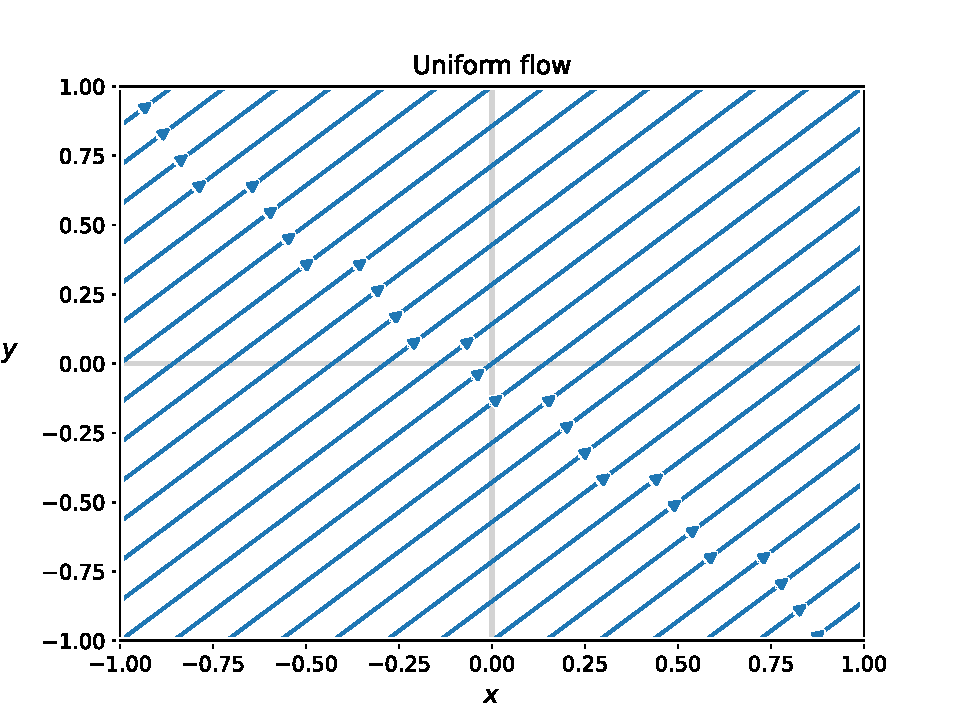
\includegraphics[width=\linewidth]{external/uniformflow.pdf}
\end{image}%
\tcblower
\end{figureptx}%
\end{example}
\begin{example}{Example}{Stagnation point flow.}{example-potential-stagnation}%
\index{stagnation point flow}%
We can verify that the velocity potential%
\begin{equation*}
\phi = \frac{1}{2} (x^2 - y^2),
\end{equation*}
satisfies Laplace's equation. The corresponding velocity field is given by%
\begin{equation*}
[u, v] = [x, -y]. 
\end{equation*}
and corresponds to \emph{stagnation point flow}.%
\par
The streamlines (or velocity field) is shown below.%
\begin{figureptx}{Figure}{Streamlines (or velocity field) of stagnation point flow.}{fig-potential-stagnation}{}%
\begin{image}{0.05}{0.9}{0.05}{}%
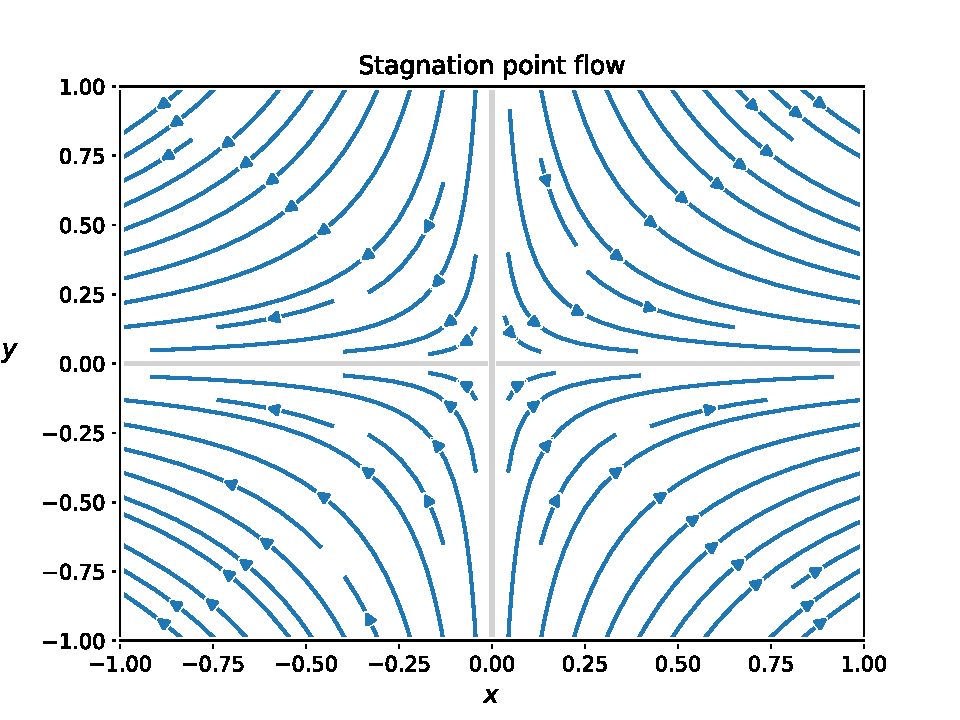
\includegraphics[width=\linewidth]{external/stagnationflow.pdf}
\end{image}%
\tcblower
\end{figureptx}%
\end{example}
\begin{example}{Example}{Line source.}{example-potential-linesource}%
\index{line source}%
We aim to derive the potential and velocity for a \emph{line source}, imagined as the flow consisting of a point source or point sink that ejects\slash{}drains fluid from a point in space. Since it would be expected for the potential to be axisymmetric, we attempt to solve \(\nabla^2 \phi = 0\) in plane polar coordinates. This is given by%
\begin{equation*}
\nabla^2 \phi = \frac{1}{r} \pd{}{r}\left(r \pd{\phi}{r}\right) + \frac{1}{r^2} \pd{^2 \phi}{\theta^2} = 0.
\end{equation*}
We assume that the potential takes the form \(\phi = \phi(r)\). Then direct integration gives%
\begin{equation*}
\phi = \frac{Q}{2\pi} \log r, 
\end{equation*}
where we have set an additional constant of integration to zero without loss of generality. The leading constant has been set to \(Q/(2\pi)\) so that \(Q\) can be later identified with a physical quantity.%
\par
The velocity then follows from consideration of the gradient in polar form,%
\begin{equation*}
\bu = \nabla \phi = \pd{\phi}{r} \be_r + \frac{1}{r}\pd{\phi}{\theta} \be_{\theta} = \frac{Q}{2\pi r} \be_r,
\end{equation*}
where the unit vectors written in the Cartesian basis are \(\be_r = [\cos\theta, \sin\theta]\) and \(\be_{\theta} = [-\sin\theta, \cos\theta]\). Thus we can write the velocity as%
\begin{equation*}
\bu = \frac{Q}{2\pi r^2} r[\cos\theta, \sin\theta] = \frac{Q}{2\pi r^2} [x, y].
\end{equation*}
The above corresponds to a velocity field directed radially outwards from the origin. The flow is a called a \emph{line source} because fluid is ejected from the origin (a source). It refers to a "line" because in \((x, y, z)\), the source runs parallel to the \(z\)-axis.%
\par
The streamlines (or velocity field) are shown below.%
\begin{figureptx}{Figure}{Streamlines (or velocity field) of line source flow.}{fig-potential-linesource}{}%
\begin{image}{0.05}{0.9}{0.05}{}%
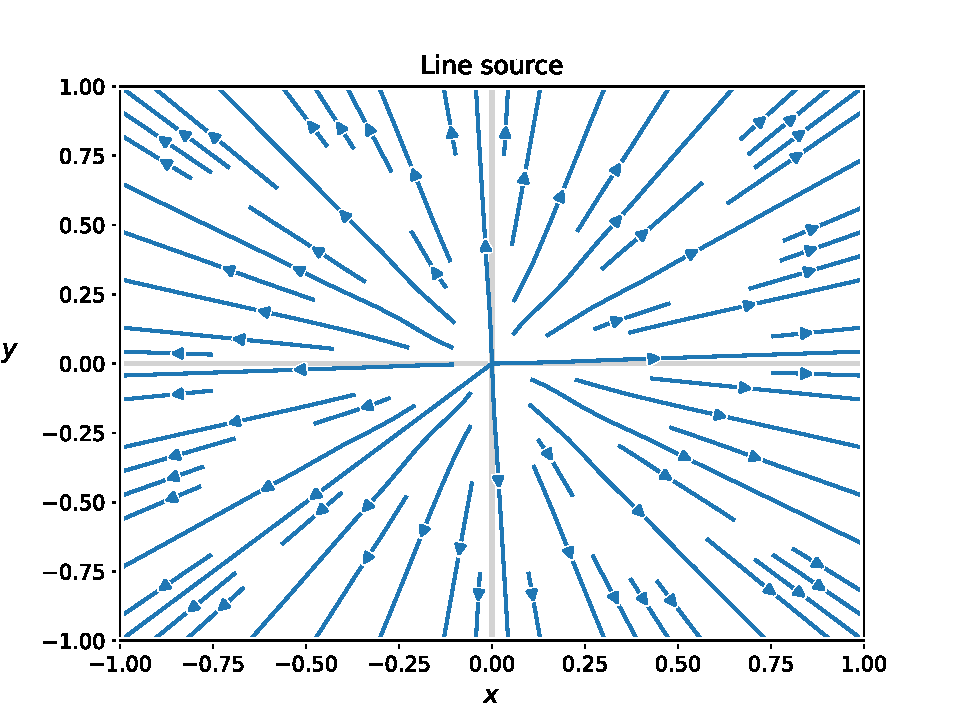
\includegraphics[width=\linewidth]{external/linesource.pdf}
\end{image}%
\tcblower
\end{figureptx}%
Let us also identify the \emph{strength} of this line source. Consider a closed contour \(C\) around the origin. Then the quantity%
\begin{equation*}
\int_C \bu \cdot \bn \, \de{s},
\end{equation*}
is the flux (the flow per unit time) of fluid crossing the contour, with \(\bn\) denoting the unit normal along \(C\).%
\par
For simplicity, let us take the contour \(C\) to be a circle of constant radius \(r = a\). Then since the unit normal is precisely \(\be_r\), we have that%
\begin{equation*}
\int_C \bu \cdot \bn \, \de{s} = \int_0^{2\pi} \frac{Q}{2\pi a} \be_r \cdot \be_r \, (a \, \de\theta) = Q. 
\end{equation*}
In computing the above integral, remember that the conversion following the polar Jacobian is \(\de{s} = r \de{\theta}\) where \(r = a\).%
\par
Therefore, \(Q\) is the rate at which fluid is produced from the line source. If \(Q \lt 0\), we refer to the flow as a \emph{line sink}. \index{line sink}%
\end{example}
Crucially, because the governing fluid mechanical equation is only Laplace's equation: this is a linear partial differential equation, and therefore the summation of elementary flows also produces an admissible flow.%
\begin{example}{Example}{Line source in a uniform flow.}{example-potential-movingsource}%
For instance, we may combine a uniform flow in the \(x\)-direction with a line source:%
\begin{equation*}
\phi = Ux + \frac{Q}{2\pi} \log r = Ux + \frac{Q}{2\pi} \log \sqrt{x^2 + y^2}.
\end{equation*}
We can then obtain the velocity field as%
\begin{equation*}
\bu = [U, 0] + \frac{Q}{2\pi(x^2 + y^2)} [x, y].
\end{equation*}
%
\par
The streamlines (or velocity field) is shown below.%
\begin{figureptx}{Figure}{Streamlines (or velocity field) of a line source in a uniform flow with \(U = 1\) and \(Q = 1\).}{fig-potential-movinglinesource}{}%
\begin{image}{0.05}{0.9}{0.05}{}%
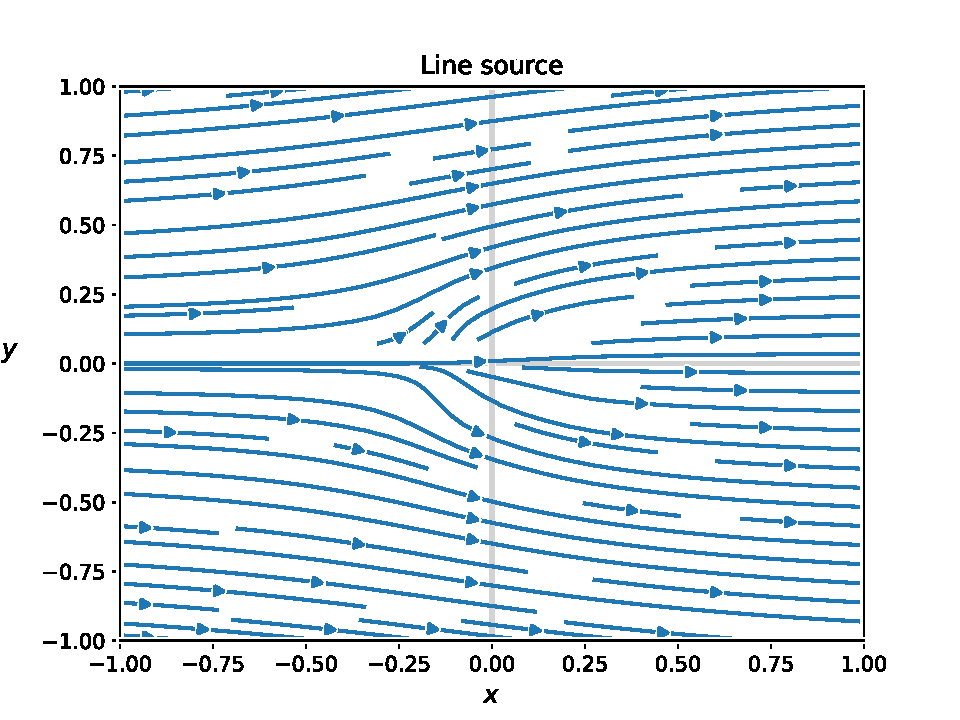
\includegraphics[width=\linewidth]{external/movinglinesource.pdf}
\end{image}%
\tcblower
\end{figureptx}%
Where do you think the stagnation point lies in this flow?%
\end{example}
\end{subsectionptx}
\end{sectionptx}
%
%
\typeout{************************************************}
\typeout{Section 4.2 The streamfunction}
\typeout{************************************************}
%
\begin{sectionptx}{Section}{The streamfunction}{}{The streamfunction}{}{}{ch-chapter04-potentialflows-4}
\begin{introduction}{}%
Our next task is to introduce the concept of the \emph{streamfunction}. Remember that in 2D, the irrotational flow led to the equation \hyperref[eqn-2d-irrotational]{({\xreffont\ref{eqn-2d-irrotational}})} and this led to the existence of the potential function. If we begin with incompressibility, however, we have \hyperref[eqn-2d-divu]{({\xreffont\ref{eqn-2d-divu}})}, which can be written as%
\begin{equation}
\nabla \times [-v, u] = 0.\label{eqn-1d-divu-cross}
\end{equation}
And we can deduce the existence of an analogous function, the \emph{streamfunction}, \(\psi(x, y, t)\) satisfying,%
\begin{equation}
u = \pd{\psi}{y} \quad \textrm{and} \quad v = -\pd{\psi}{x}.\label{eqn-2d-uv-streamfunction}
\end{equation}
Alternatively and more conveniently, we can write%
\begin{equation}
\bu = \nabla \times (\psi \bk).\label{eqn-2d-streamfunction}
\end{equation}
To establish the existence of the streamfunction, we follow a similar proof as in \hyperref[thm-exist-potential]{Theorem~{\xreffont\ref{thm-exist-potential}}} but now with the definition that%
\begin{equation}
\psi(x, y, t) = \psi_0(t) + \int_0^{\bx} (u \de{y} - v \de{x}),\label{eqn-streamfunction-def-psi}
\end{equation}
where again \(\psi_0(t)\) is an arbitrary function of \(t\). The proof is otherwise identical, relying on establishing the independence of path of the integral using Stokes' theorem.%
\par
Why all this work? The streamfunction has an intuitive intepretation via the following result.%
\begin{theorem}{Theorem}{The streamfunction is constant along streamlines.}{}{thm-streamfunction}%
The streamfunction, \(\psi(x, y, t)\), is constant along streamlines of the flow (i.e. the trajectory formed by a particle in the flow).%
\end{theorem}
\begin{proof}{Proof}{}{thm-streamfunction-3}
The proof follows simply by the fact that%
\begin{equation*}
\bu \cdot \nabla \psi = \left(\pd{\psi}{y}, -\pd{\psi}{x}\right) \cdot \left(\pd{\psi}{x}, \pd{\psi}{y}\right) = 0,
\end{equation*}
and for which the substitution in the first equality follows from \hyperref[eqn-2d-uv-streamfunction]{({\xreffont\ref{eqn-2d-uv-streamfunction}})}.%
\par
The above equality indicates that the velocity vector, \(\bu\), is orthogonal to the vector pointing along \(\nabla \psi\). However, it is known from Vector Calculus that \(\nabla \psi\) runs along curves of steepest descent\slash{}ascent of \(\psi\)-{}-{}-these must hence be orthogonal to the level sets of \(\psi\). Therefore, the level sets of \(\psi\) are tangential to \(\bu\) (the definition of a streamline).%
\end{proof}
A graphical depiction of the property in \hyperref[thm-streamfunction]{Theorem~{\xreffont\ref{thm-streamfunction}}} is shown below.%
\begin{figureptx}{Figure}{Flow between two streamlines, where the streamlines \(\psi_1\) and \(\psi_2\) are constant. Later, we will consider the flux through the contour \(C\) illustrated in the figure along with its unit normal \(\bn\).}{fig-streamfunction}{}%
\begin{image}{0.15}{0.7}{0.15}{}%
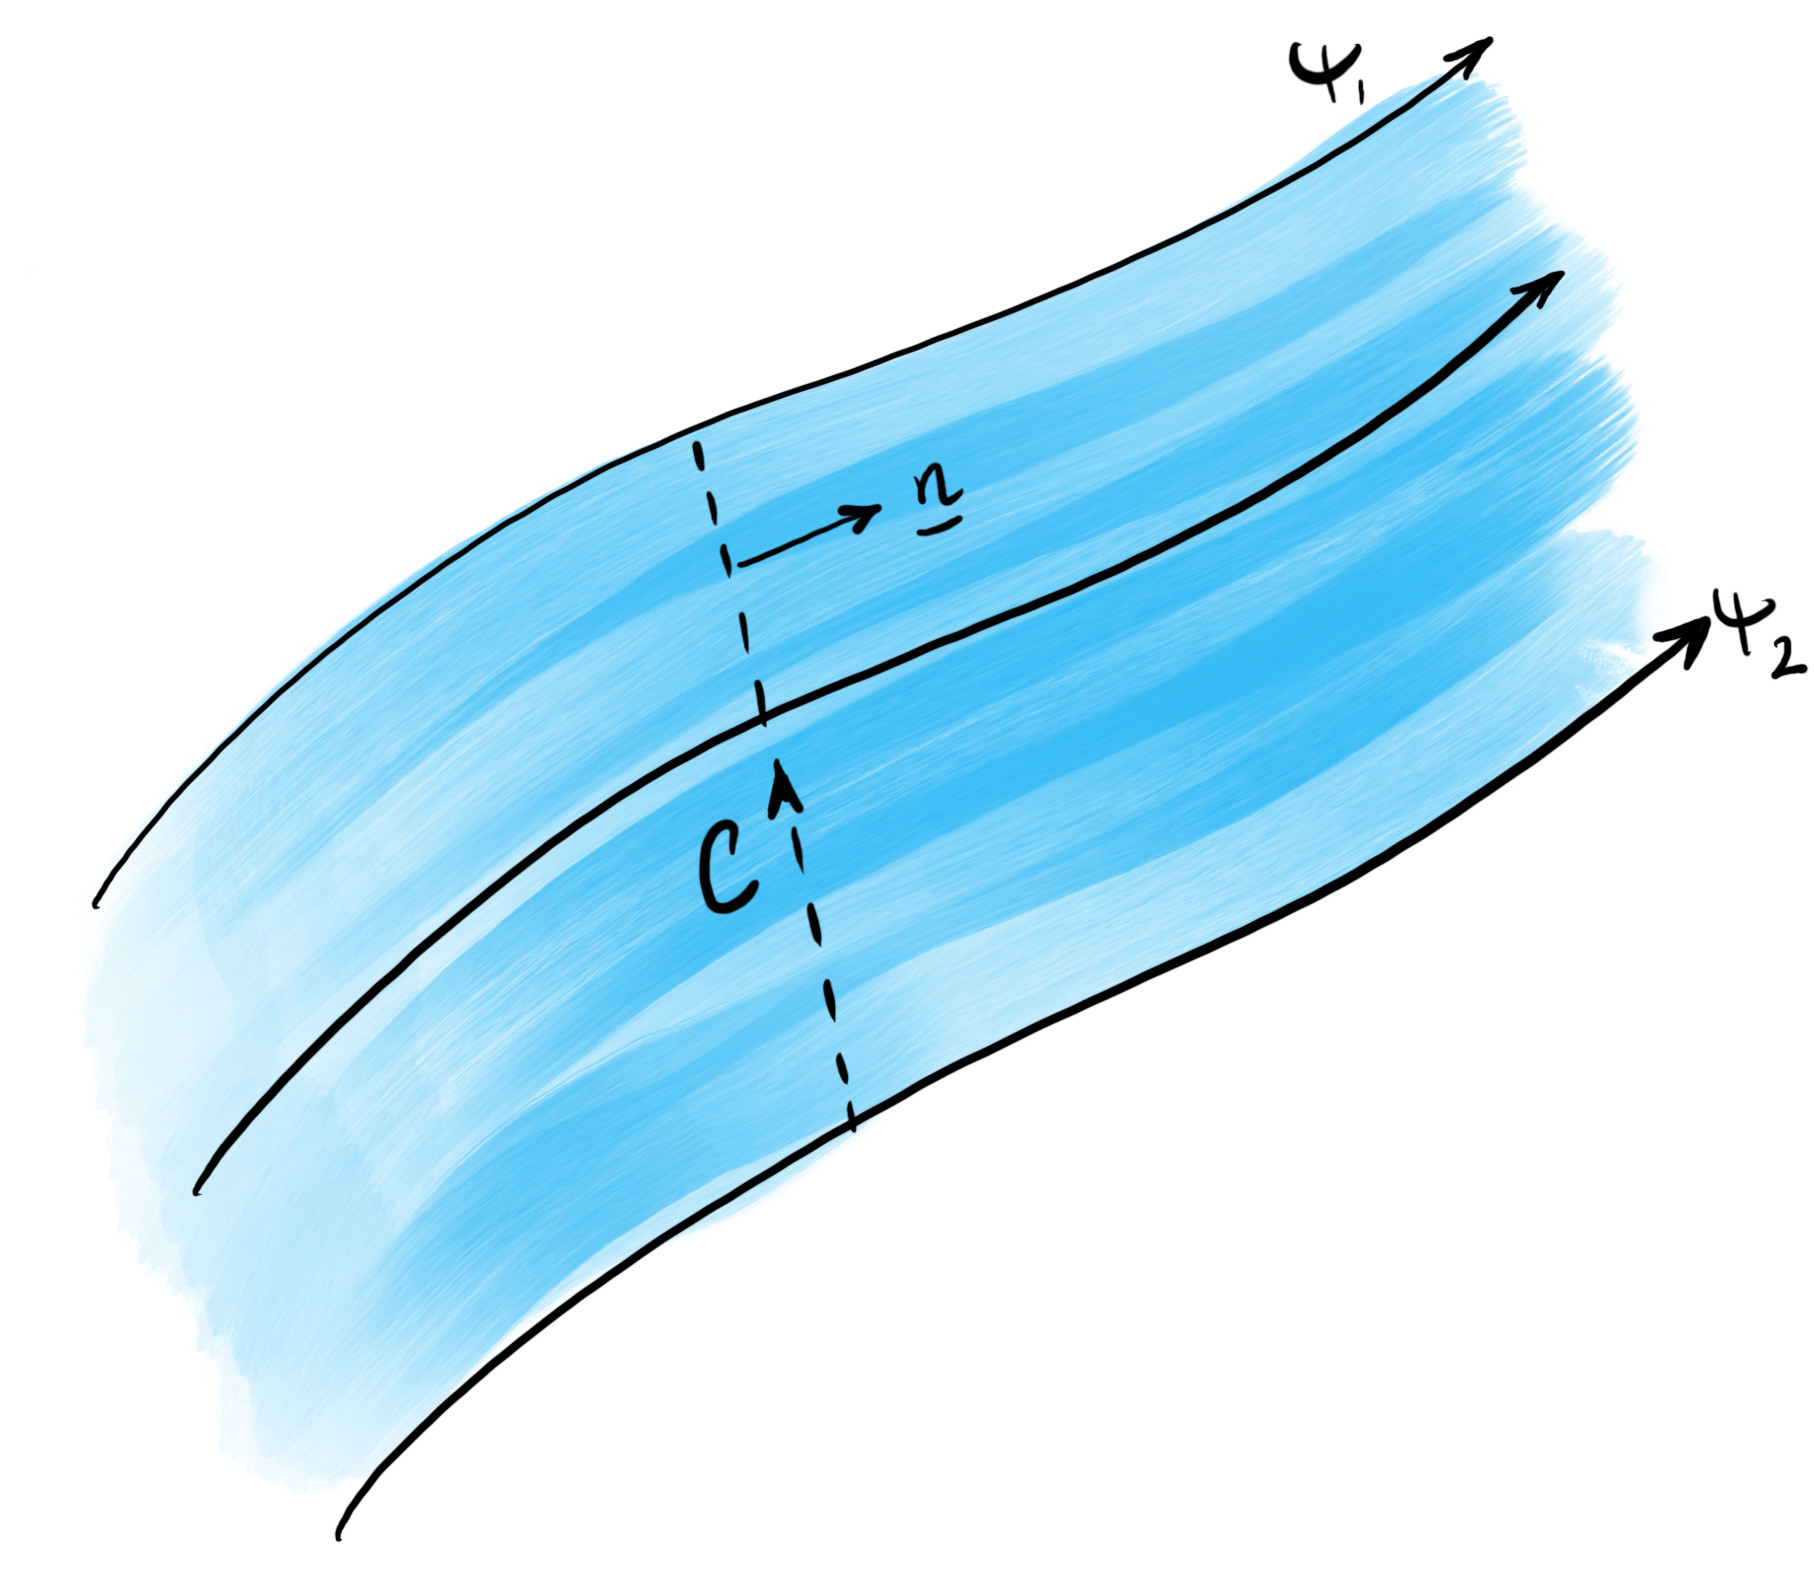
\includegraphics[width=\linewidth]{external/streamfunction.jpg}
\end{image}%
\tcblower
\end{figureptx}%
The streamfunction is thus constant on streamlines. Consider two streamlines. The following theorem relates the flux between the streamlines to the streamline values.%
\begin{theorem}{Theorem}{Flux between streamlines.}{}{thm-flux-streamlines}%
Consider streamlines \(\psi = \psi_1\) and \(\psi = \psi_2\). The \emph{flux} (net flow of fluid) between the two streamlines is given by%
\begin{equation*}
\textrm{flux} = \psi_1 - \psi_2.
\end{equation*}
%
\end{theorem}
\begin{proof}{Proof}{}{thm-flux-streamlines-3}
By definition, the flux is given by the integral%
\begin{equation*}
\int_C \bu \cdot \bn \, \de{s},
\end{equation*}
where \(C\) is any smooth path joining the two streamlines with unit normal \(\bn\), as shown in FIGURE.%
\par
Note that given the curve, the unit normal is written as \([-\de{y}, \de{x}]/\de s\), so \(\bn \de{s} = [\de{y}, -\de{x}]\). Then the flux is re-written as the following:%
\begin{align*}
\textrm{flux} \amp= \int_C \left[\pd{\psi}{y}, -\pd{\psi}{x}\right] \cdot [\de{y}, \de{x}], \\
\amp= \int_C \left(\pd{\psi}{x} \, \de{x} + \pd{\psi}{y} \right), \\
\amp= \bigl[ \psi \bigr]_C, \\
\amp= \psi_2 - \psi_1. 
\end{align*}
In the third line above, \([\psi]_C\) is the change of \(\psi\) across the contour. Note that there is somewhat an arbitrary choice of direction for the contour \(C\), as related to the selection of the normal direction \(\bn\), and the positivity or negativity of the flux.%
\end{proof}
Finally, note that the velocity potential was governed by Laplace's equation, \(\nabla^2 \phi = 0\). The streamfunction is also governed by the same Laplace's equation.%
\begin{theorem}{Theorem}{Streamfunction satisfies Laplace's equation.}{}{thm-streamfunction-laplace}%
Like the velocity potential, the streamfunction satisfies Laplace's equation:%
\begin{equation}
\pd{^2 \psi}{x^2} + \pd{^2 \psi}{y^2} = \nabla^2 \psi = 0.\label{eqn-2d-streamfunction-laplace}
\end{equation}
%
\end{theorem}
\begin{proof}{Proof}{}{thm-streamfunction-laplace-3}
Substitute the relationship \hyperref[eqn-2d-uv-streamfunction]{({\xreffont\ref{eqn-2d-uv-streamfunction}})} into \hyperref[eqn-2d-irrotational]{({\xreffont\ref{eqn-2d-irrotational}})}.%
\end{proof}
Like in the situation of certain flows, e.g. the line source in \hyperref[example-potential-linesource]{Example~{\xreffont\ref{example-potential-linesource}}}, it is easier to work in alternative coordinate systems to study the streamfunction. Since we know that \(\bu = \nabla \times (\psi \bk)\) by \hyperref[eqn-2d-streamfunction]{({\xreffont\ref{eqn-2d-streamfunction}})}, we can use the conversion of the curl to polar coordinates in \hyperref[eqn-identity-curlpolar]{({\xreffont\ref{eqn-identity-curlpolar}})} to give%
\begin{equation}
u_r = \frac{1}{r} \pd{\psi}{\theta} \quad \textrm{and} \quad u_{\theta} = -\pd{\psi}{r}\,\label{eqn-streamfunction-polar}
\end{equation}
which allows us to relate the radial and angular velocities to the streamfunction.%
\end{introduction}%
%
%
\typeout{************************************************}
\typeout{Subsection 4.2.1 Elementary flows}
\typeout{************************************************}
%
\begin{subsectionptx}{Subsection}{Elementary flows}{}{Elementary flows}{}{}{ch-chapter04-potentialflows-4-3}
Let us return to each of the examples in \hyperref[sec-Potential-and-streamfunction]{Section~{\xreffont\ref{sec-Potential-and-streamfunction}}} and reconsider their corresponding streamfunctions.%
\begin{example}{Example}{Uniform flow.}{ch-chapter04-potentialflows-4-3-3}%
\index{uniform flow, streamfunction}%
From \hyperref[example-potential-uniform]{Example~{\xreffont\ref{example-potential-uniform}}}, we can directly integrate \(u = \psi_y\) and \(v = -\psi_x\) to get%
\begin{equation*}
\psi = Uy\cos\alpha - Ux\sin\alpha, 
\end{equation*}
up to an arbitrary constant. Therefore, lines of constant \(\psi\) correspond to%
\begin{equation*}
y = x\tan\alpha + \textrm{constant},
\end{equation*}
which indeed yields the image seen in \hyperref[fig-potential-uniform]{Figure~{\xreffont\ref{fig-potential-uniform}}}.%
\end{example}
\begin{example}{Example}{Stagnation point flow.}{ch-chapter04-potentialflows-4-3-4}%
\index{stagnation point flow, streamfunction}%
Now turning to \hyperref[example-potential-stagnation]{Example~{\xreffont\ref{example-potential-stagnation}}}, we integrate \(u = y = \psi_x\) and \(v = x = \psi_y\). This gives%
\begin{equation*}
\psi = xy, 
\end{equation*}
up to an arbitrary constant. Indeed curves of constant \(\psi\) match the hyperbole shown in \hyperref[fig-potential-stagnation]{Figure~{\xreffont\ref{fig-potential-stagnation}}}.%
\end{example}
\begin{example}{Example}{Line source.}{example-streamfunction-linesource}%
\index{line source, streamfunction}%
For the situation of the line source in \hyperref[example-potential-linesource]{Example~{\xreffont\ref{example-potential-linesource}}}, we want to work with polar coordinates. From the previous work, we have for this situation the potential \(\phi = Q/(2\pi log r\). It then follows from the polar version of the gradient in \hyperref[eqn-identity-grad-polar]{({\xreffont\ref{eqn-identity-grad-polar}})}, that the velocity is entirely radial and%
\begin{equation}
\bu = \pd{\phi}{r}\be_r + 0 = \frac{Q}{2\pi r} \be_r.\label{eqn-streamfunction-u-linesource}
\end{equation}
We use the formulae in \hyperref[eqn-streamfunction-polar]{({\xreffont\ref{eqn-streamfunction-polar}})} and integrate \(\frac{1}{r} \pd{\psi}{\theta} = \frac{Q}{2\pi r}\) yielding%
\begin{equation*}
\psi = \frac{Q}{2\pi} \theta.
\end{equation*}
Then indeed note that the lines of constant \(\psi\) are given by the radial lines of constant \(\theta\), matching the illustration in \hyperref[fig-potential-linesource]{Figure~{\xreffont\ref{fig-potential-linesource}}}.%
\end{example}
Another remark concerns the fact that \(\psi\) is a multi-valued function in the example of the line source \hyperref[example-streamfunction-linesource]{Example~{\xreffont\ref{example-streamfunction-linesource}}}, gaining a jump of \(Q\) every time the origin is encircled. This is indeed a warning that the standard proof, analogous to \hyperref[thm-exist-potential]{Theorem~{\xreffont\ref{thm-exist-potential}}}, leading to the existence of a unique streamfunction, via \hyperref[eqn-streamfunction-def-psi]{({\xreffont\ref{eqn-streamfunction-def-psi}})} would not apply since the velocity field \hyperref[example-streamfunction-linesource]{Example~{\xreffont\ref{example-streamfunction-linesource}}} is not defined at the origin. However, despite this, we see that the streamfunction provides well-defined predictions of streamlines on the \emph{cut} plane with e.g. \(\theta \in [0, 2\pi)\).%
\begin{example}{Example}{Line source in a uniform flow.}{ch-chapter04-potentialflows-4-3-7}%
Like the case of the potential function in \hyperref[example-potential-movingsource]{Example~{\xreffont\ref{example-potential-movingsource}}}, the linearity of the equation governing the streamfunction implies that we can consider the combination of those streamfunctions for a line source with a uniform flow. This yields%
\begin{equation*}
\psi = Uy + \frac{Q}{2\pi}\theta, 
\end{equation*}
for the case of uniform flow of speed \(U\) in the positive \(x\)-direction. The streamlines are then given by%
\begin{equation*}
Uy + \frac{Q}{2\pi} \theta = \frac{Q}{2\pi}C,
\end{equation*}
having designed the constant combination on the right hand-side for convenience. Then using \(y = r\sin\theta\), we have%
\begin{equation*}
r = \left(\frac{Q}{2\pi U}\right) \frac{C - \theta}{\sin\theta}.
\end{equation*}
%
\end{example}
Our previous examples were reliant on considering the flows generated by the velocity potentials studied previously. However, we can also consider "fundamental solutions" of the equation \(\nabla^2 \psi = 0\) in their own right. Recall that in deriving the velocity potential of the line source in \hyperref[example-potential-linesource]{Example~{\xreffont\ref{example-potential-linesource}}}, we considered the solution of an axi-symmetric problem, where \(\phi = \phi(r)\) is only dependent on the distance from the origin. A similar argument must imply that the analogous axi-symmetric streamfunction is a permissible solution. And this leads us to the following example.%
\begin{example}{Example}{Line vortex.}{example-streamfunction-linevortex}%
\index{line vortex}%
The fundamental solution for the streamfunction, in plane polar coordinates, is the axisymmetric solution,%
\begin{equation}
\psi = -\frac{\Gamma}{2\pi}\log r,\label{eqn-streamfunction-linevortex}
\end{equation}
defined up to a constant, and corresponds to a \emph{line vortex}.%
\par
The streamlines of such a flow correspond to circular trajectories with \(r\) constant, and are visualised in %
\begin{figureptx}{Figure}{Streamlines (or velocity field) of a line vortex with \(\Gamma = 1\).}{fig-streamfunction-linevortex}{}%
\begin{image}{0.05}{0.9}{0.05}{}%
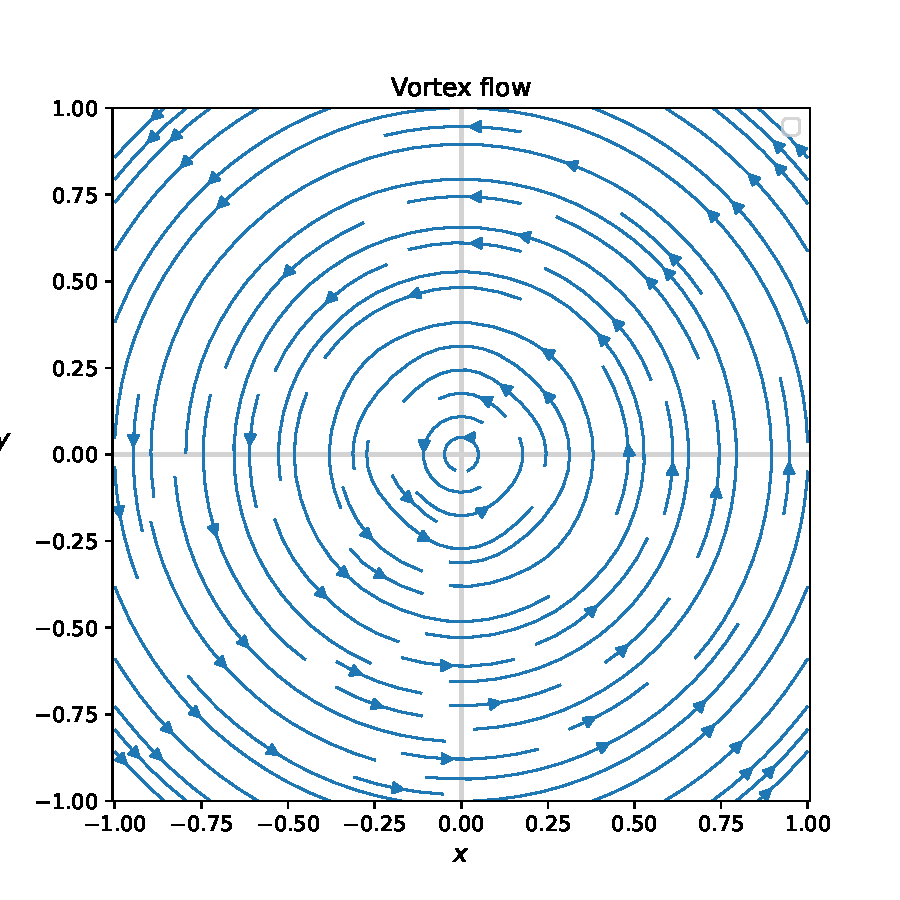
\includegraphics[width=\linewidth]{external/linevortex.pdf}
\end{image}%
\tcblower
\end{figureptx}%
Recall that the radial and angular velocities are given by \hyperref[eqn-streamfunction-polar]{({\xreffont\ref{eqn-streamfunction-polar}})}. Therefore, we see that the velocity vector is given by%
\begin{equation*}
\bu = -\pd{\psi}{r} \be_{\theta} = \frac{\Gamma}{2\pi r} \be_{\theta},
\end{equation*}
and thus this flow corresponds to entirely circular trajectories orbiting the origin, and with angular velocity increasing as \(r \to 0\).%
\par
The quantity \(\Gamma\) is called the \emph{vortex strength}, analogous to the source strength \(Q\) in \hyperref[example-potential-linesource]{Example~{\xreffont\ref{example-potential-linesource}}}. Let us consider the amount of circulation around a contour \(C\) that contains the origin:%
\begin{equation*}
\oint_C \bu \cdot \de{\bx} = \oint_C (u \, \de{x} + v \, \de{y}),
\end{equation*}
i.e. one envisions encircling the origin along \(C\), adding up each of the velocity components tangential to the path. This is the circulation. By Stokes' theorem it is equal to the flux of vorticity of the corresponding bounding surface.%
\par
Choosing \(C\) to be the circle of radius \(r = a\), we have \(\de{\bx} = a \be_{\theta} \de{\theta}\). Then the circulation is given by%
\begin{equation*}
\oint_C \bu \cdot \de{\bx} = \int_0^{2\pi} \frac{\Gamma}{2\pi a} \be_{\theta} \cdot \be_{\theta} a \de\theta = \Gamma.
\end{equation*}
So indeed this gives us an intuitive understanding of \(\Gamma\). Notice that \(\Gamma \gt 0\) corresponds to flow in the anticlockwise sense, and \(\Gamma \lt 0\) corresponds to flow in the clockwise sense.%
\end{example}
\end{subsectionptx}
\end{sectionptx}
%
%
\typeout{************************************************}
\typeout{Section 4.3 The complex potential}
\typeout{************************************************}
%
\begin{sectionptx}{Section}{The complex potential}{}{The complex potential}{}{}{sec-complex-potential}
\begin{introduction}{}%
In the previous two sections, we studied the properties and utility of the velocity potential \(\phi\) and streamfunction \(\psi\) in the context of two-dimensional potential flows (inviscid, incompressible, irrotational). We did this with techniques from real-valued Vector Calculus.  As it turns out, there is a much more elegant and powerful framework for studying two-dimensional flow which leverages the significant power of complex analysis and complex variables.%
\par
In fact, you may have already noticed this on an intuitive level, given the intimate relationships between \(\phi\) and \(\psi\), seeming to exhibit a certain kind of symmetry in formulae and operations. Complex analysis is the language in which we can make this kind of "symmetry" transparent.%
\par
We begin by reviewing (or in some cases, introducing) you to some key theorems about the properties of well-behaved (analytic) complex functions.%
\par
In his section, we will refer to a complex function generically as%
\begin{equation*}
f(z) = u(x, y) + \im v(x, y)
\end{equation*}
where \(u\) and \(v\) and the real-valued decompositions of the complex-valued function \(f\). Also, \(z = x + \im y\).%
\par
A complex function is differentiated in much the same way as real-valued functions, with the definition that%
\begin{equation}
f'(z) = \lim_{\Delta z \to 0} \frac{f(z + \Delta z) - f(z)}{\Delta z}.\label{eqn-complex-derivative}
\end{equation}
The crucial difference with real-valued differentiation is that the above limit is required to hold whilst approaching the point \(z\) in any direction of the complex plane.%
\begin{remark}{Remark}{}{sec-complex-potential-2-6}%
As long as you stay away from exceptional points of a function, the "calculus" of complex functions is largely the same as for real-valued functions, e.g.%
\begin{gather*}
\dd{(z^m)}{z} = mz^{m-1}, \qquad \dd{\e^z}{z} = \e^z,\\
\dd{(\log (z+1))}{z} = \frac{1}{z + 1}, \quad \dd{\sin(z^2)}{z} = 2z\cos(z^2). 
\end{gather*}
and the usual rules of algebraic manipulations hold. There are some caveats, however, which are dealt with on an individual manner.%
\end{remark}
Below, we will often use susbcripts for partial differentiation, e.g. \(u_x = \pd{u}{x}\).%
\end{introduction}%
%
%
\typeout{************************************************}
\typeout{Subsection 4.3.1 Cauchy's theorem and harmonic functions}
\typeout{************************************************}
%
\begin{subsectionptx}{Subsection}{Cauchy's theorem and harmonic functions}{}{Cauchy's theorem and harmonic functions}{}{}{subsec-complex-introduction}
We will follow the reference text by \hyperlink{ref-kreyszig}{[{\xreffont 2}]} and \hyperlink{ref-fornberg}{[{\xreffont 6}]}  and introduce the basic notions of complex functions that we will need.%
\begin{definition}{Definition}{Analyticity.}{def-analytic}%
\index{analytic}%
A function \(f: \mathbb{C} \to \mathbb{C}\) is said to be analytic in a domain if \(f(z)\) is defined and differentiable at all points in the domain. The function is said to be \emph{analytic at a point} \(z = z_0\) if it is analytic in a neighbourhood of \(z_0\).%
\par
When we refer to an \emph{analytic function}, we mean a function that is analytic in some domain of \(\mathbb{C}\) (often clear by context).%
\par
The function is \emph{holomorphic}\index{holomorphic} if it is analytic; the terms are synonyms.%
\par
An analytic function is \emph{entire}\index{entire} if its region of analyticity includes all points in \(\mathbb{C}\), including infinity.%
\end{definition}
Note that above, we have stated that a function is analytic if it is well-defined and differentiable \emph{once}(!) As it turns out, the requirement that a complex-valued function is differentiable is a strong condition. An analytic function turns out to be infinitely differentiable by consequence!%
\begin{remark}{Remark}{}{subsec-complex-introduction-5}%
In this module, we will not be concerned with formalities when they are not relevant. For example, in our definition of analyticity, we do not specify if the relevant domains are open or closed. The functions we work with are generally non-pathological-{}-{}-they may have isolated singularities or exceptional points, but generally the application and context will make it clear the limits of our results.%
\end{remark}
Now we have one of the most important theorems of complex analysis.%
\begin{theorem}{Theorem}{Cauchy-Riemann equations I.}{}{thm-CR1}%
If \(f(z) = u(x, y) + \im v(x, u)\) is differentiable, then the Cauchy-Riemann equations, given by%
\begin{equation}
u_x = v_y \quad \text{and} \quad u_y = -v_x,\label{eqn-CR}
\end{equation}
hold.%
\par
In particular, if \(f\) is analytic on a domain, then its real and complex parts must satisfy the Cauchy-Riemann equations \hyperref[eqn-CR]{({\xreffont\ref{eqn-CR}})} (in that domain).%
\end{theorem}
\begin{proof}{Proof}{}{thm-CR1-3}
(Non-examinable)%
\par
This follows by considering the definition of the derivative \hyperref[eqn-complex-derivative]{({\xreffont\ref{eqn-complex-derivative}})} when the point \(z\) is approached from the \(x\) or \(y\) directions.%
\par
With \(\Delta z = \Delta x\) real, we can verify from applying the definition that%
\begin{equation*}
f'(z) = \pd{u}{x} + \im \pd{v}{x}.
\end{equation*}
On the other hand, approaching with \(\Delta z = \im \Delta y\) gives%
\begin{equation*}
f'(z) = -\im \pd{u}{y} + \pd{v}{y}. 
\end{equation*}
Equating the two results then yields the Cauchy-Riemann equations.%
\end{proof}
It turns out that the Cauchy-Riemann equations are not only necessary to an analytic function, but are actually sufficient as well.%
\begin{theorem}{Theorem}{Cauchy-Riemann equations II.}{}{thm-CR2}%
If two real-valued continuous functions, \(u(x, y)\) and \(v(x, y)\) of two real variables \(x\) and \(y\) have continuous firsst partial derivatives that satisfy the Cauchy-Riemann equations \hyperref[eqn-CR]{({\xreffont\ref{eqn-CR}})} in some domain, then \(f(z0 = u(x, y) + \im v(x, y)\) is analytic in that domain.%
\end{theorem}
\begin{proof}{Proof}{}{thm-CR2-3}
(Non-examinable)%
\par
The proof is not difficult, but we will refer students to \hyperlink{ref-kreyszig}{[{\xreffont 2}]} for its proof. It relies on constructing the derivative of \(f\) along any direction using the decomposition into the two Cartesian directions.%
\end{proof}
\begin{theorem}{Theorem}{}{}{thm-complex-inf-derivatives}%
If \(f\) is analytic, it is differentiable to all orders.%
\end{theorem}
Our last step involves relating complex functions to the solution of Laplace's equation(s), i.e. \hyperref[eqn-2d-laplace]{({\xreffont\ref{eqn-2d-laplace}})} or \hyperref[eqn-2d-streamfunction-laplace]{({\xreffont\ref{eqn-2d-streamfunction-laplace}})}, that govern potential flow.%
\begin{theorem}{Theorem}{Analyticity and Laplace's equation.}{}{thm-complex-laplace}%
If \(f(z) = u(x, y) + \im v(x, y)\) is analytic in a domain \(D\), then \(u\) and \(v\) satisfy Laplace's equation,%
\begin{equation*}
\nabla^2 u = u_{xx} + u_{yy} = 0 \quad \textrm{and} \quad
\nabla^2 v = v_{xx} + v_{yy} = 0,
\end{equation*}
in \(D\), and have continuous second partial derivatives in \(D\).%
\end{theorem}
\begin{proof}{Proof}{}{thm-complex-laplace-3}
Since \(f\) is analytic, then it follows from \hyperref[thm-CR1]{Theorem~{\xreffont\ref{thm-CR1}}} that \(u_x = v_y\) and \(u_y = -v_x\). It furthermore follows from \hyperref[thm-complex-inf-derivatives]{Theorem~{\xreffont\ref{thm-complex-inf-derivatives}}} that \(f\) is differentiable to all orders; therefore, we can take derivatives to obtain%
\begin{equation*}
u_{xx} = v_{yx} \quad \text{and} \quad -u_{yy} = v_{xy}. 
\end{equation*}
The second derivatives are continuous and therefore \(v_{xy} = v_{yx}\). Therefore \(u_{xx} + u_{yy} = 0\). Laplace's equation is analogously proved for \(v\).%
\end{proof}
The above theorem is truly a remarkable result; it would not be a stretch to state that this single result was at the forefront of why complex analysis played such an important role in the development of applied mathematics and physics in the 18th, 19th, and 20th centuries.%
\par
Since Laplace's equation, \(\nabla^2 \phi = 0\), is such an important equation in physics, occuring in theories of gravitation, electrostatics, fluid mechanics, etc. the theorem establishes that there exists a parallel theory in the language of complex variables for the specific case of two-dimensional applications.%
\par
A potential fluid, for example, can be studied by manipulating complex functions of the form%
\begin{equation*}
f(z) = \phi(x, y) + \im \psi(x, y).
\end{equation*}
One can envision all kinds of different forms of \(f\)-{}-{}-polynomials, cosines and sines, exponentials, logarithms, etc. As long as the function is locally differentiable, it is thus analytic and therefore can be associated with (some kind of) fluid flow.%
\end{subsectionptx}
%
%
\typeout{************************************************}
\typeout{Subsection 4.3.2 Examples of elementary flows}
\typeout{************************************************}
%
\begin{subsectionptx}{Subsection}{Examples of elementary flows}{}{Examples of elementary flows}{}{}{subsec-complex-examples}
Let us return to the examples of flows studied in \hyperref[sec-Potential-and-streamfunction]{Section~{\xreffont\ref{sec-Potential-and-streamfunction}}} and re-interpret them using the theory of analytic functions.%
\par
We will associate the velocity potential, \(\phi\), and streamfunction \(\psi\) with an analytic function in the following way.%
\begin{definition}{Definition}{}{def-complex-potential}%
Let \(\phi(x,y)\) and \(\psi(x, y)\) be the respective velocity potential and streamfunction for some potential flow. We define%
\begin{equation}
f(z) = \phi(x, y) + \im \psi(x, y),\label{eqn-complex-potential}
\end{equation}
and call \(f\) the \emph{complex potential}.%
\par
Note that by differentiating in the horizontal and vertical directions, we have%
\begin{equation*}
\dd{f}{z} = \pd{}{x} (\phi + \im \psi) = \pd{}{y} (\phi + \im \psi). 
\end{equation*}
Therefore it follows that the horizontal and vertical velocity components of the flow, related via \(\bu = [u, v]\), are given by%
\begin{equation}
\dd{f}{z} = u - \im v.\label{eqn-complex-velocity}
\end{equation}
%
\end{definition}
\begin{example}{Example}{Uniform flow.}{subsec-complex-examples-5}%
\index{uniform flow, complex}%
We can verify that the complex potential for uniform flow is given from%
\begin{equation*}
f(z) = U \e^{-\im \alpha} z.
\end{equation*}
This can be compared to  \hyperref[example-potential-uniform]{Example~{\xreffont\ref{example-potential-uniform}}}.%
\end{example}
\begin{example}{Example}{Stagnation point flow.}{subsec-complex-examples-6}%
\index{stagnation point flow, complex}%
We can verify that the complex potential for a stagnation point flow is given by%
\begin{equation*}
f(z) = \frac{z^2}{2}.
\end{equation*}
This can be compared to  \hyperref[example-potential-stagnation]{Example~{\xreffont\ref{example-potential-stagnation}}}.%
\end{example}
\begin{example}{Example}{Line source.}{subsec-complex-examples-7}%
\index{line source, complex}%
We can verify that the complex potential for a line source flow is given by%
\begin{equation}
f(z) = \frac{Q}{2\pi} \log z\label{eqn-complex-linesource}
\end{equation}
This can be compared to  \hyperref[example-potential-linesource]{Example~{\xreffont\ref{example-potential-linesource}}}.%
\par
The complex logarithm is an example of a function that is not analytic at the isolated point \(z = 0\) where it possesess a \emph{branch point}. However, it still provides a permissible analytic function away from the origin.%
\par
The evaluation of the complex logarithm can be performed via the definition%
\begin{equation}
\log z = \log r + \im \theta,\label{eqn-complex-logarithm}
\end{equation}
where \(z = r\e^{\im \theta}\) is the polar form representation of \(z\). In particular \(log z\) is a multi-function with a \emph{branch point} at the origin.%
\par
With the above decomposition of the logarithm in mind, notice that we can then conclude that the velocity potential and streamfunction are given by%
\begin{equation*}
\phi = \Re[f] = \frac{Q}{2\pi} \log r \quad \text{and} \quad
\psi = \Im[f] = \frac{Q}{2\pi} \theta.
\end{equation*}
Indeed the streamlines are along the rays \(\theta\) constant.%
\par
From \hyperref[eqn-complex-linesource]{({\xreffont\ref{eqn-complex-linesource}})}, we can also compute the velocities using the relationship \hyperref[eqn-complex-velocity]{({\xreffont\ref{eqn-complex-velocity}})}. We thus have%
\begin{equation*}
u - \im v = \frac{Q}{2\pi} \frac{1}{z} = \frac{Q}{2\pi} \frac{x - \im y}{(x^2 + y^2)},
\end{equation*}
once we have multiplied the top and bottom by the conjugate of \(z\).%
\end{example}
\begin{example}{Example}{Line vortex flow.}{subsec-complex-examples-8}%
\index{line vortex, complex}%
We can verify that the complex potential for a line vortex is given by%
\begin{equation*}
f(z) = -\frac{\im \Gamma}{2\pi} \log z.
\end{equation*}
This can be compared to  \hyperref[example-streamfunction-linevortex]{Example~{\xreffont\ref{example-streamfunction-linevortex}}}.%
\par
Again, using the definition of the complex logarithm, via \hyperref[eqn-complex-logarithm]{({\xreffont\ref{eqn-complex-logarithm}})}, we can write \(f\) in terms of its real and complex components as%
\begin{equation*}
f(z) = \frac{\Gamma}{2\pi} (\theta - \im \log r),
\end{equation*}
where \(z = r\e^{\im\theta}\)\textgreater{}. Therefore, the streamfunction is given by \(\psi = -(\Gamma/2\pi) \log r\) and is constant along circular trajectories with constant distance from the origin, \(r\).%
\end{example}
\end{subsectionptx}
\end{sectionptx}
%
%
\typeout{************************************************}
\typeout{Section 4.4 The method of images}
\typeout{************************************************}
%
\begin{sectionptx}{Section}{The method of images}{}{The method of images}{}{}{sec-method-of-images}
\begin{introduction}{}%
The preceeding sections would give the misleading impression that solving potential-flow problems for two-dimensional flows is easy. This is not the case, and the primary reason is due to the presence of \emph{boundary conditions}. The elementary flows we have previously considered were unconfined and\slash{}or we did not consider additonal constraints on their behaviours at infinity. In reality, a real physical fluid, whether in the ocean, the air, or in a container, is confined in some direction, and we must often consider subtle questions about the mechanism that produces the fluid motion.%
\par
In this section, we consider the situation of solving for the potential flow in a fluid region with boundaries. Recall that this is equivalent to finding a velocity potential satisfying \(\nabla^2 \phi = 0\) or an analytic complex potential, \(f(z)\).%
\par
Recall from \hyperref[note-noflux-BC]{Note~{\xreffont\ref{note-noflux-BC}}} that on solid boundaries, we must impose the no-flux condition that%
\begin{equation*}
\bu \cdot \bn = \nabla \phi \cdot \bn = 0 \quad \text{on $\partial V$}.
\end{equation*}
%
\end{introduction}%
%
%
\typeout{************************************************}
\typeout{Subsection 4.4.1 Planar boundaries: a half-plane}
\typeout{************************************************}
%
\begin{subsectionptx}{Subsection}{Planar boundaries: a half-plane}{}{Planar boundaries: a half-plane}{}{}{subsec-images-planar}
Consider the situation illustrated in \hyperref[image-planar01]{Figure~{\xreffont\ref{image-planar01}}}.%
\begin{figureptx}{Figure}{Blah}{image-planar01}{}%
\begin{image}{0.1}{0.8}{0.1}{}%
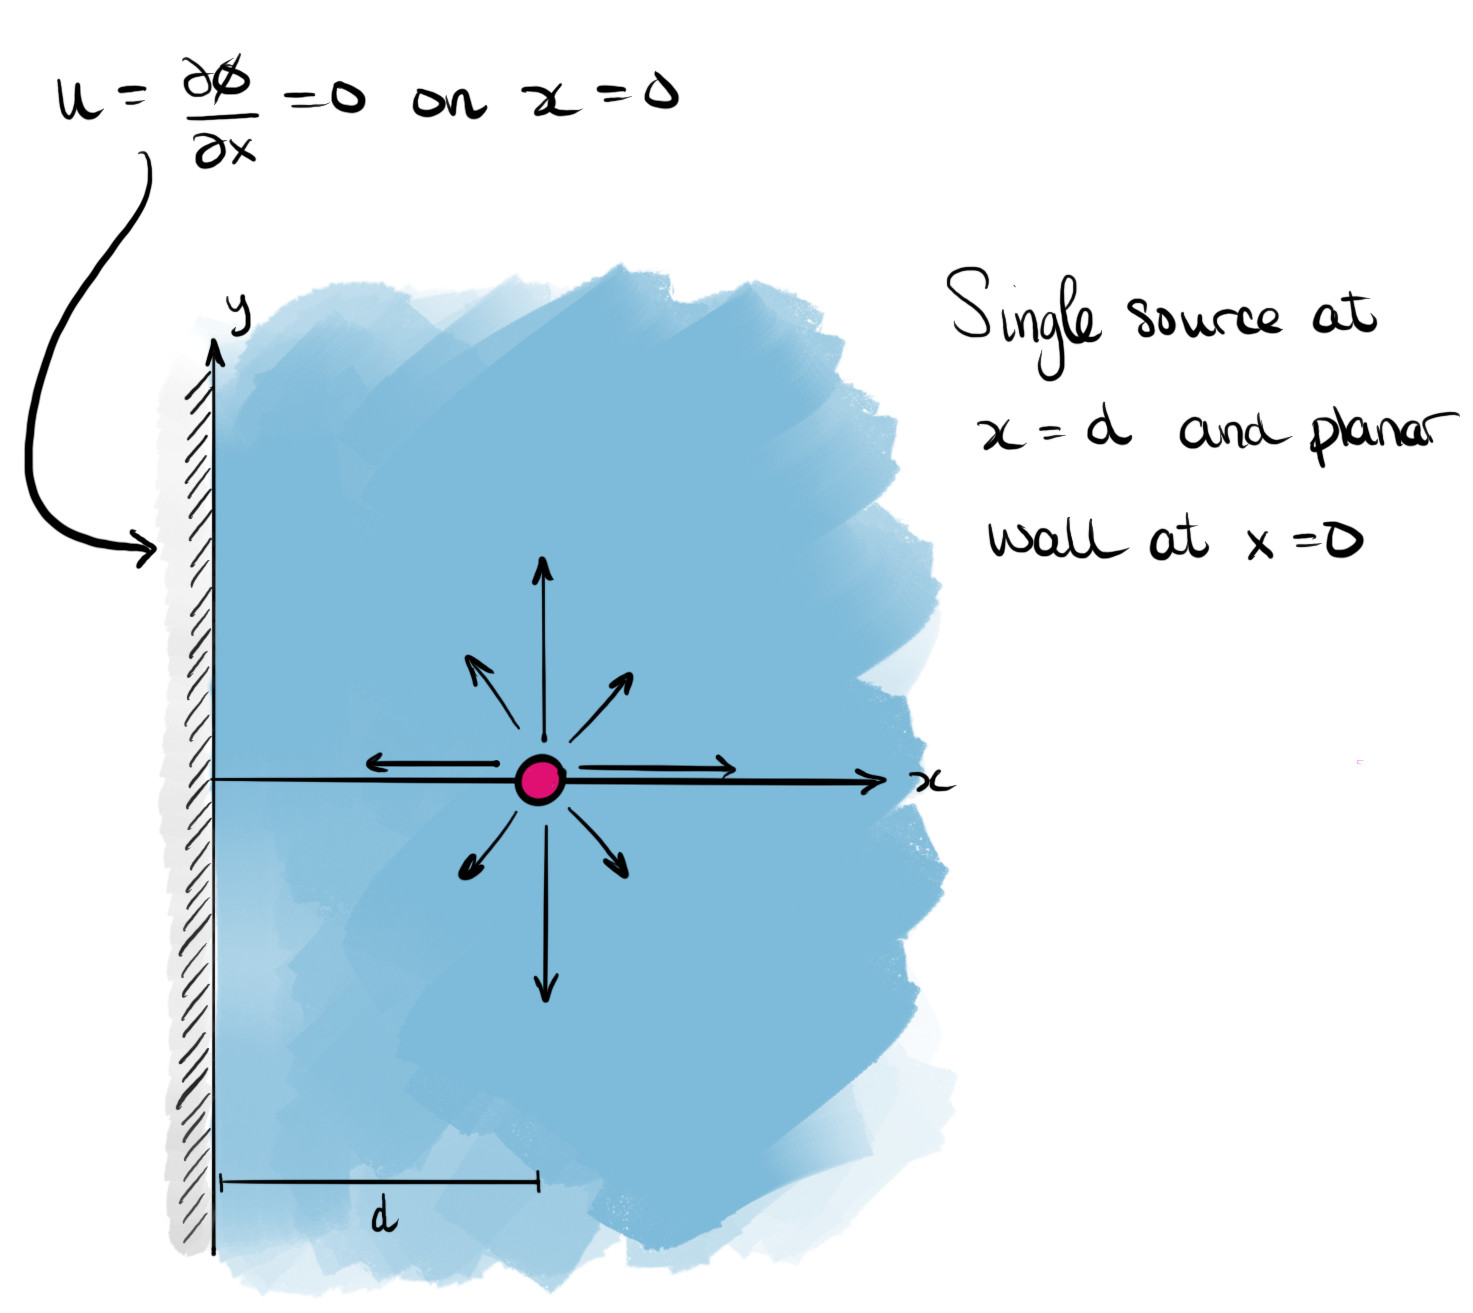
\includegraphics[width=\linewidth]{external/image-planar01.jpg}
\end{image}%
\tcblower
\end{figureptx}%
We envision a semi-infinite region of fluid bounded on the left by a wall at \(x = 0\). A single (line) source of strength \(Q\) is placed at \(x = d\). Therefore from \hyperref[eqn-complex-linesource]{({\xreffont\ref{eqn-complex-linesource}})}, we would expect that at least near \(x = d\), the complex potential behaves as%
\begin{equation*}
f(z) \sim \frac{Q}{2\pi} \log (z-d) \quad \text{as $z \to d$}.
\end{equation*}
However the above solution does not satisfy the required boundary conditions at \(x = 0\) since it corresponds to a velocity field for which the horizontal velocity penetrates through \(x = 0\). This can be verified via inspection. For example, we can inspect the velocity or the streamlines; this is part of \hyperlink{ps-image-planar01}{Exercise~{\xreffont 4.6.1}}.%
\par
Rephrased in terms of the streamlines, the boundary condition at \(x = 0\) is equivalent to the constraint that%
\begin{equation*}
\Im f(z) = \psi = \textrm{constant at $x = 0$}.
\end{equation*}
%
\par
Our inspired solution to the above problem is referred to as \emph{the method of images}.%
\begin{note}{Note}{Method of images.}{note-method-of-images}%
Given potential flow problem, we consider the superposition of elementary sinks\slash{}sources, i.e.%
\begin{equation*}
f(z) = \frac{1}{2\pi} \sum_{j=0}^{N-1} Q_j \log(z - z_j), 
\end{equation*}
and\slash{}or vortices,%
\begin{equation*}
f(z) = -\frac{\im}{2\pi} \sum_{j=0}^{N-1} \Gamma_j \log(z - z_j).
\end{equation*}
The strengths and locations of the individual contributions are chosen so that boundary conditions on the required boundaries (including at infinity) can be met.%
\end{note}
Notice that the \emph{linearity} of the potential flow problem is crucial: any analytic function is associated with a velocity potential that satisfies Laplace's equation, \(\nabla^2 \phi = 0\), and therefore the superposition of such functions also yields a permissible complex potential, \(f\).%
\par
We consider the addition of a "fictitious" image source, with the same strength at the reflected point \(x = -d\), which lies outside of the posited fluid region. This gives the complex potential of%
\begin{equation*}
f(z) = \frac{Q}{2\pi} \log(z - d) + \frac{Q}{2\pi} \log(z + d). 
\end{equation*}
This yields the illustration of the flow in \hyperref[fig-image-planar02]{Figure~{\xreffont\ref{fig-image-planar02}}}%
\begin{figureptx}{Figure}{Blah}{fig-image-planar02}{}%
\begin{image}{0.1}{0.8}{0.1}{}%
\includegraphics[width=\linewidth]{external/image-planar02.jpg}
\end{image}%
\tcblower
\end{figureptx}%
The corresponding complex velocity is given by%
\begin{equation*}
u - \im v = f'(z) = \frac{Q}{2\pi}\frac{z}{z^2 - d^2}.
\end{equation*}
So indeed, on the central boundary, we have \(z = \im y\), and%
\begin{equation*}
u - \im v = - \im \frac{Q}{\pi} \frac{y}{y^2 + d^2},
\end{equation*}
and the velocity is entirely vertical. So indeed, the condition that \(\bu \cdot \bn = 0\) on the planar boundary is satisfied.%
\par
In order to study the complex velocity, \(f(z)\), and develop an equation for the streamlines of the flow, we must first navigate the fact that the complex logarithm function is only well-defined in a slit complex plane. First, let%
\begin{equation*}
z - d = r_1 \e^{\im \theta_1} \quad \textrm{and} \quad z + d = r_2 \e^{\im \theta_2}.
\end{equation*}
Using the definition of the complex logarithm \hyperref[eqn-complex-logarithm]{({\xreffont\ref{eqn-complex-logarithm}})}, we have%
\begin{equation*}
f(z) = \frac{Q}{2\pi} \left[ \log r_1 + \log r_2\right] + \im \frac{Q}{2\pi}\left[ \theta_1 + \theta_2 \right].
\end{equation*}
The definitions of \(r_1, r_2\) and \(\theta_1, \theta_2\), are shown in the below figure. In order for each logarithm to be well defined, the angles \(\theta_1\) and \(\theta_2\) must be restricted to be less than a complete revolution. We thus restrict \(\theta_1 \in [0, 2\pi)\) and \(\theta_1 \in [-\pi, \pi)\).%
\begin{figureptx}{Figure}{Blah}{fig-image-duallog}{}%
\begin{image}{0}{1}{0}{}%
\includegraphics[width=\linewidth]{external/image-duallog.jpg}
\end{image}%
\tcblower
\end{figureptx}%
In \hyperlink{ps-image-planar02}{Exercise~{\xreffont 4.6.2}}, you will be asked to develop an equation for the streamlines of this flow.%
\par
The above ideas can be extended to the situation of a line vortex in a half plane. Again, we are interested in describing the flow due to a line vortex at \(z = d\), and therefore we expect that near this point,%
\begin{equation*}
f(z) \sim -\frac{\im\Gamma}{2\pi} \log(z - d) \quad \textrm{as $z \to d$}.
\end{equation*}
However, the above potential does not satisfy the necessary zero-flux condition at \(x = 0\).%
\par
In this case, the approach is to add an image vortex at \(z = -d\), but opposite in direction:%
\begin{equation*}
f(z) = -\frac{\im\Gamma}{2\pi} \log(z - d) + \frac{\im\Gamma}{2\pi} \log(z + d).
\end{equation*}
Therefore, this flow is composed by a line vortex circulating anticlockwise on the right, and a line vortex circulating clockwise on the left. It can be verified that the complex velocity is given by%
\begin{equation*}
u - \im v = -\frac{\im \Gamma d}{\pi(z^2 - d^2)}
\end{equation*}
and indeed the velocity at \(x = 0\) is entirely vertical and there is no flux through the boundary.%
\par
There is an exercise in \hyperlink{ps-image-planar03}{Exercise~{\xreffont 4.6.3}}.%
\begin{remark}{Remark}{Uniqueness of solutions.}{subsec-images-planar-18}%
You may be wondering: if a permissible potential function is found that satisfies the necessary boundary conditions, can we be certain it is the unique solution in the problem (up to a constant)? You may understand the construction of potentials, via the method of images, but perhaps irked that it involves the insertion of these so-called 'fictitious' points. The answer, at least for most non-pathological problems in potential flow theory (i.e. all the problems you study) is \emph{yes}, the solution you have found is assured to be the only solution (up to a constant).%
\par
This is, to some extent, related to the \href{https://proofwiki.org/wiki/Uniqueness_of_Analytic_Continuation}{uniqueness of analytic continuation}. In a nutshall, the relevant theorem states that given two admissible complex potentials, say \(f_1(z)\) and \(f_2(z)\), that agree on the line \(x = 0\) (in the case of the above situation), it is the case that \(f_1 = f_2\) everywhere (where they are analytic).%
\par
Therefore, you can be certain that solutions you find via the trick of method of images are the only solutions.%
\end{remark}
\end{subsectionptx}
\end{sectionptx}
%
%
\typeout{************************************************}
\typeout{Section 4.5 Conformal mapping}
\typeout{************************************************}
%
\begin{sectionptx}{Section}{Conformal mapping}{}{Conformal mapping}{}{}{sec-conformal-mapping}
\begin{introduction}{}%
The essential idea of conformal mapping is as follows. Suppose that we are given a two-dimensional potential fluid flow problem in a region, \(R \subseteq \mathbb{C}\), with impermeable boundary \(\partial R\). There may be singularities in \(R\) corresponding to sinks, sources, vortices, etc. We then seek a \emph{conformal mapping} from the \(z\)-plane to the \(\zeta\)-plane via%
\begin{equation*}
\zeta = g(z),
\end{equation*}
so that the region \(R\) is mapped to a new region \(\hat{R} \subseteq \mathbb{C}\), as shown in \hyperref[fig-conformal-general]{Figure~{\xreffont\ref{fig-conformal-general}}}.%
\par
The hope is that within the \(\zeta\)-plane, the fluid region is sufficiently simple that a complex potential, say \(F(\zeta)\), can be found. This task is aided by virtue of the fact that sinks\slash{}sources and vortices are preserved by the conformal map. Typically, we wish for \(\hat{R}\) to be e.g. the upper half-plane or the unit disc, with \(\partial\hat{R}\) to be the real axis or circumferance of the unit disc, respectively. Once found, the complex potential in the \(z\)-plane is then obtained simply by inverting the conformal map, i.e.%
\begin{equation*}
f(z) = F(g(\zeta)) = \phi(x, y) + \im \psi(x, y).
\end{equation*}
This simple idea turns out to yield many insights to potential flows in two dimensions.%
\begin{figureptx}{Figure}{A general conformal mapping from the \(z\)-plane to the \(\zeta\)-plane. The object is to map the region \(R\) to the region \(\hat{R}\), which is geometrically simpler.}{fig-conformal-general}{}%
\begin{image}{0}{1}{0}{}%
\includegraphics[width=\linewidth]{external/conformal_generalmap.jpg}
\end{image}%
\tcblower
\end{figureptx}%
\end{introduction}%
%
%
\typeout{************************************************}
\typeout{Subsection 4.5.1 Source in a wedge}
\typeout{************************************************}
%
\begin{subsectionptx}{Subsection}{Source in a wedge}{}{Source in a wedge}{}{}{sec-conformal-mapping-3}
Consider fluid contained in a wedge with walls at \(\theta = 0\) and \(\theta = \alpha > 0\), and with the fluid in \(0 < \theta < \alpha\). A source of strength \(Q\) is placed somewhere within the flow, say at the point \(z = c\).%
\par
Consider then the map%
\begin{equation}
\zeta = g(z) = z^{\pi/\alpha}.\label{eqn-conformal-wedge-map}
\end{equation}
It can be verified that this map transforms the fluid region to the upper half-\(\zeta\)-plane. Indeed the ray \(\theta = 0\) is mapped to the positive real axis and the ray \(\theta = \alpha\) is mapped to the negative real axis. This is shown in \hyperref[fig-conformal-wedge]{Figure~{\xreffont\ref{fig-conformal-wedge}}}.%
\begin{figureptx}{Figure}{The map from the wedge-shaped region in the \(z\)-plane (left) and the upper half-\(\zeta\)-plane (right).}{fig-conformal-wedge}{}%
\begin{image}{0}{1}{0}{}%
\includegraphics[width=\linewidth]{external/conformal_wedge.jpg}
\end{image}%
\tcblower
\end{figureptx}%
In the \(\zeta\)-plane, the fluid problem thus consists of solving for flow in the upper half-plane with a source of strength \(Q\) at the location \(\zeta = c^{\pi/\alpha} = \zeta_c\), with an impermeable boundary on the real \(\zeta\)-axis. Indeed, from the previous section, we know this can be solved using the method of images, with a source placed at both the point \(\zeta_c\) and its complex conjugate point, \(\overline{\zeta_c}\). It then follows that the complex potential is%
\begin{equation}
F(\zeta) = \frac{Q}{2\pi} \log(\zeta - \zeta_c) + \frac{Q}{2\pi} \log(\zeta - \overline{\zeta_c}).\label{eqn-conformal-zeta-wedge}
\end{equation}
We can then invert the above formula, expressing the complex potential in the \(z\)-plane as%
\begin{equation}
f(z) = F(g(z)) = \frac{Q}{2\pi} \log(z^{\pi/\alpha} - c^{\pi/\alpha}) + \frac{Q}{2\pi} \log(z^{\pi/\alpha} - \overline{c^{\pi/\alpha}}).\label{eqn-conformal-z-wedge}
\end{equation}
%
\par
We can verify with a computational plot that this complex potential indeed seems to duplicate the necessary fluid flow within the wedge.%
\end{subsectionptx}
%
%
\typeout{************************************************}
\typeout{Subsection 4.5.2 The conformal mapping method}
\typeout{************************************************}
%
\begin{subsectionptx}{Subsection}{The conformal mapping method}{}{The conformal mapping method}{}{}{subsec-conformal-theory}
How does it work?%
\par
We can say that the conformal mapping method is dependent on a number of key properties of conformal maps.%
\begin{definition}{Definition}{Conformal map.}{def-conformal-mapping}%
Let us specifically define a \emph{conformal map} as a mapping, \(\zeta = g(z)\), where \(g\) is analytic in a region \(R\) and also that \(\dd{g}{z} \neq 0\) in \(R\).%
\end{definition}
The following properties hold for conformal maps.%
\begin{proposition}{Proposition}{Properties of conformal maps.}{}{prop-conformal}%
%
\begin{enumerate}
\item{}Conformal maps preserve angles.%
\item{}If the boundary \(\partial{\hat{R}}\) is a streamline in the \(\zeta\)-plane, then the corresponding boundary \(\partial R\) is a streamline in the \(z\)-plane (and vice versa).%
\item{}A source (or vortex) of strength \(Q\) at \(\zeta = g(c) \in \hat{R}\) in the \(\zeta\)-plane corresponds to a source (or vortex) of the same strength \(Q\) at \(z = c \in R\) in the \(z\)-plane (and vice versa).%
\end{enumerate}
%
\end{proposition}
\end{subsectionptx}
%
%
\typeout{************************************************}
\typeout{Subsection 4.5.3 Standard conformal maps}
\typeout{************************************************}
%
\begin{subsectionptx}{Subsection}{Standard conformal maps}{}{Standard conformal maps}{}{}{sec-conformal-mapping-5}
The \emph{exponential map} is used to map a channel to a half-space. Consider a channel of width \(h\) in the region \(0 < \Im z < h\) in the \(z\)-plane. Then%
\begin{equation}
\zeta = g(z) = \e^{\pi z/h},\label{eqn-conformal-exp-map}
\end{equation}
maps this channel to the upper half-\(\zeta\)-plane. The correspondence of critical points and points at infinity in the pre-image and the image is shown in \hyperref[eqn-conformal-exp-map]{({\xreffont\ref{eqn-conformal-exp-map}})}. It is good to see the map as essentially 'unfolding' the infinite channel, sending points AD to the origin, while sending B to negative infinity and C to positive infinity. The conformal map will preserve the orientation of the boundary, so as we traverse along ABCD, the fluid region is always on the left.%
\begin{figureptx}{Figure}{The exponential map maps the infinite strip of height \(h\) to the upper half-plane.}{fig-conformal-exp}{}%
\begin{image}{0}{1}{0}{}%
\includegraphics[width=\linewidth]{external/conformal_exp.jpg}
\end{image}%
\tcblower
\end{figureptx}%
\emph{Trigonometric maps} are used to map semi-infinite channels into a half space. Consider for example, the region \(R\) given in the following diagram in \hyperref[eqn-conformal-sin-map]{({\xreffont\ref{eqn-conformal-sin-map}})}. We can then see that the semi-infinite channel of width \(2a\) has been mapped to the upper half-plane. The two corners at \(z = \pm a\) have been mapped to \(\zeta = \pm 1\), respectively.%
\begin{figureptx}{Figure}{The exponential maps the infinite strip of height \(h\) to the upper half-plane.}{fig-conformal-sin}{}%
\begin{image}{0}{1}{0}{}%
\includegraphics[width=\linewidth]{external/conformal_sin.jpg}
\end{image}%
\tcblower
\end{figureptx}%
The above map is given by%
\begin{equation}
\zeta = g(z) = \sin\left(\frac{\pi z}{2a}\right).\label{eqn-conformal-sin-map}
\end{equation}
%
\begin{example}{Example}{Vortex flow in a semi-infinite channel.}{sec-conformal-mapping-5-7}%
Consider the channel shown in the left of \hyperref[fig-conformal-sinh]{Figure~{\xreffont\ref{fig-conformal-sinh}}}. Insert a vortex of strength \(\Gamma\) at the point \(z = d \in \mathbb{R^+}\). Verify that an appropriate conformal map is given by%
\begin{equation}
\zeta = g(z) = \textrm{sinh}\left(\frac{\pi z}{2a}\right),\label{eqn-conformal-sinh}
\end{equation}
and find where the map sends the relevant critical points of the pre-image.%
\par
Using the conformal map, find the complex velocity of the flow.%
\begin{figureptx}{Figure}{The exponential maps the infinite strip of height \(h\) to the upper half-plane.}{fig-conformal-sinh}{}%
\begin{image}{0}{1}{0}{}%
\includegraphics[width=\linewidth]{external/conformal_sinh.jpg}
\end{image}%
\tcblower
\end{figureptx}%
\end{example}
\end{subsectionptx}
\end{sectionptx}
%
%
\typeout{************************************************}
\typeout{Exercises 4.6 Exercises}
\typeout{************************************************}
%
\begin{exercises-section}{Exercises}{Exercises}{}{Exercises}{}{}{ws-potentialflows}
\begin{introduction}{}%
\begin{warning}{Warning}{}{ws-potentialflows-1-1}%
We look to complete worksheets in the week prior to the content being delivered. Once this is done, this disclaimer message will be removed.%
\end{warning}
\end{introduction}%
\begin{divisionexercise}{1}{Single source in a semi-infinite flow.}{}{ps-image-planar01}%
Verify that a single source of strength \(Q\) placed at the point \(z = d > 0\) is insufficient to describe flow bounded in the semi-infinite region, \(x > 0\), with a planar boundary at \(x = 0\). What is the horizontal and vertical velocities on the boundary? Find an equation for the streamlines and sketch the flow.%
\end{divisionexercise}%
\begin{divisionexercise}{2}{A source in a semi-infinite flow.}{}{ps-image-planar02}%
Consider the situation of two point sources of identical strength, \(Q\), placed at \(z = \pm d\), with \(d \gt 0\). Develop equations for the complex potential, \(f(z) = \phi + \im \psi\), and complex velocity, \(u - \im v\).%
\par
Demonstrate that the streamlines are given by hyperbolae and develop the equation for their form.%
\end{divisionexercise}%
\begin{divisionexercise}{3}{Two vortices and a dividing boundary.}{}{ps-image-planar03}%
Consider the situation of two point vorticies of identical strength, but opposite direction, placed at \(z = \pm d\), with \(d \gt 0\). Develop equations for the complex potential, \(f(z) = \phi + \im \psi\), and complex velocity, \(u - \im v\).%
\par
Demonstrate that the streamlines are given by%
\begin{equation*}
\psi = \frac{\Gamma}{2\pi}\log \left( \frac{r_2}{r_1}\right).
\end{equation*}
%
\end{divisionexercise}%
\begin{divisionexercise}{4}{}{}{ps-conformal-check-exp-sin}%
Check.%
\end{divisionexercise}%
\end{exercises-section}
\end{chapterptx}
%
%
\typeout{************************************************}
\typeout{Chapter 5 Water waves}
\typeout{************************************************}
%
\begin{chapterptx}{Chapter}{Water waves}{}{Water waves}{}{}{ch-chapter05-waves}
\renewcommand*{\chaptername}{Chapter}
\begin{introduction}{}%
In this chapter, you will study the theory of linear and nonlinear water waves. Linear water waves can be obtained by series expansions of the relevant free-surface equations. Nonlinear water waves requires the use of computational methods.%
\end{introduction}%
\end{chapterptx}
%
%
\typeout{************************************************}
\typeout{Chapter 6 Vortex motion}
\typeout{************************************************}
%
\begin{chapterptx}{Chapter}{Vortex motion}{}{Vortex motion}{}{}{ch-chapter06-vorticity}
\renewcommand*{\chaptername}{Chapter}
\begin{introduction}{}%
In this chapter, we will study the motion of vortices in an inviscid fluid. We will define vortex lines, which are to the vorticity field as the streamlines defined in \hyperref[ch-chapter02-kinematics]{Chapter~{\xreffont\ref{ch-chapter02-kinematics}}} are to the velocity field. We will show that vortex lines move with the fluid and that a fluid that starts irrotational remains irrotational for all time.%
\begin{sidebyside}{3}{0}{0}{0}%
\begin{sbspanel}{0.333333333333333}%
\begin{panelfigureptx}{Figure}{A tornado (credit Greg Johnson, Unsplash).}{ch-chapter06-vorticity-2-2-1}{}%
\noindent\includegraphics[width=\linewidth]{external/ch-chapter06-greg-johnson-5V3FUicslvo-unsplash.jpg}
\tcblower
\end{panelfigureptx}%
\end{sbspanel}%
\begin{sbspanel}{0.333333333333333}%
\begin{panelfigureptx}{Figure}{Wingtip vortices behind an aircraft (credit NASA Langley Research Center).}{ch-chapter06-vorticity-2-2-2}{}%
\noindent\includegraphics[width=\linewidth]{external/ch-chapter06-NASA-Langley-Research-Center-il_wingtipvortexedit_lg.jpg}
\tcblower
\end{panelfigureptx}%
\end{sbspanel}%
\begin{sbspanel}{0.333333333333333}%
\begin{panelfigureptx}{Figure}{Vortex created when a cup of tea is stirred, also showing the secondary flow that results, which in turn leads to the \emph{tea leaf paradox} in which tea leaves sprinkled on the bottom of a cup migrate into a pile in the centre (you can try this at home). Credit Wikipedia.}{ch-chapter06-vorticity-2-2-3}{}%
\noindent\includegraphics[width=\linewidth]{external/ch-chapter06-220px-Tea_leaf_Paradox_Illustration.png}
\tcblower
\end{panelfigureptx}%
\end{sbspanel}%
\end{sidebyside}%
\par
Examples of vortex motion abound in nature and industry. The most familiar examples are perhaps tornadoes and hurricanes, which are large-scale vortices in the atmosphere. Other examples include the swirling motion that forms when water drains from a bath or sink, the wake vortices that form behind aircraft wings, and the vortices that form behind a swimming fish or a flying bird. Vortices are also important in engineering applications, for example in the design of aircraft wings and turbine blades.%
\par
Recall the fluid vorticity \(\bomega=\nabla\times\bu\) that was introduced in Definition \hyperref[def-vorticity]{Definition~{\xreffont\ref{def-vorticity}}}. Many people struggle to understand the concept of vorticity when they first encounter it, so you should not worry if it takes a while to sink in. The excellent (although dated) movie \textasciigrave{}Vorticity, Part 1’ by Ascher Shapiro available at \href{https://web.mit.edu/hml/ncfmf.html}{this website} gives a clear and comprehensive introduction to the phenomenon. To recap:%
\begin{itemize}[label=\textbullet]
\item{}Vorticity, \(\bomega\), is a vector field and it is a function of space and time (like the fluid velocity).%
\item{}At each point in the fluid, \(\bomega\) points in the direction of the axis of the local fluid rotation.%
\item{}The magnitude of \(\bomega\) is twice the local angular velocity.%
\item{}In the special case of a two-dimensional flow (that is \(\bu(\bx,t)=(u(x,y,t),v(x,y,t),0)\)), the vorticity is unidirectional, pointing in the \(z\)-direction with magnitude%
\begin{equation*}
\pd{v}{x}-\pd{u}{y}\text{.}
\end{equation*}
%
\end{itemize}
%
\begin{example}{Example}{Steady two-dimensional vortex flow.}{ex-vorticity-intro}%
Consider the steady, two-dimensional flow given by%
\begin{equation*}
\bu = (-y,x, 0)\text{,}
\end{equation*}
which is flow anti-clockwise around the origin. Note that this flow is a type of \emph{rigid body rotation}: it is the flow that would be generated by a rigid body rotating about the \(z\)-axis with angular velocity \(1\).%
\par
%
\begin{enumerate}
\item{}Plot the streamlines of this flow.%
\item{}Convert this flow to plane polar coordinates \((r,\theta)\) (where \(x = r\cos\theta\) and \(y = r\sin\theta\)), and show that the \(r\)-component of the velocity is zero and the \(\theta\)-component is \(1\).%
\item{}Hence find the angular velocity of the fluid.%
\item{}Calculate the vorticity of the flow.%
\end{enumerate}
%
\par\smallskip%
\noindent\textbf{\blocktitlefont Solution}.\hypertarget{ex-vorticity-intro-3}{}\quad{}The answers are as follows.%
\begin{enumerate}
\item{}The streamlines satisfy the differential equation%
\begin{equation*}
\dd{\bx}{s}=\bu(\bx(s)),
\end{equation*}
where \(s\) is a parameter along the streamline. In components, this reads%
\begin{equation*}
\dd{x}{s}=-y, \quad \dd{y}{s}=x.
\end{equation*}
Differentiating the first equation with respect to \(s\) and using the second gives%
\begin{equation*}
\dd{^2x}{s^2}=-\dd{y}{s}=-x,
\end{equation*}
which has general solution \(x=A\cos s + B\sin s\). Using the first equation then gives \(y=A\sin s - B\cos s\). Thus the streamlines are circles around the origin, given by \(x^2+y^2=A^2+B^2\).%
\item{}We have%
\begin{equation*}
\dd{r}{t}=\frac{x}{r}(-y)+\frac{y}{r}(x)=0,
\end{equation*}
and%
\begin{align*}
\dd{\theta}{t}\amp=\dd{}{t}\left(\tan^{-1}\frac{y}{x}\right)\\
\amp=\frac{1}{1+y^2/x^2}\left(-\frac{y}{x^2}\right)(-y)+\frac{1}{1+y^2/x^2}\left(\frac{1}{x}\right)(x)\\
\amp=1.
\end{align*}
Thus, in plane polar coordinates, the velocity is \((0,1)\).%
\item{}The angular velocity is everywhere \((0,0,1)\).%
\item{}The vorticity of the flow is given by%
\begin{equation*}
\bomega = \bnabla\times\bu
= \begin{vmatrix}
\bi \amp \bj \amp \bk \\
\pd{}{x} \amp \pd{}{y} \amp \pd{}{z} \\
-y \amp x \amp 0
\end{vmatrix}
= (0,0,2),
\end{equation*}
which is twice the local angular momentum (magnitude twice the rotation rate, with axis in the direction of the axis of rotation).%
\end{enumerate}
%
\end{example}
\end{introduction}%
%
%
\typeout{************************************************}
\typeout{Section 6.1 The Helmholtz principle}
\typeout{************************************************}
%
\begin{sectionptx}{Section}{The Helmholtz principle}{}{The Helmholtz principle}{}{}{sec-helmholtz}
\begin{introduction}{}%
As mentioned in Chapter \hyperref[ch-chapter03-equations]{Chapter~{\xreffont\ref{ch-chapter03-equations}}}, the vorticity obeys the vorticity equation \hyperref[eqn-vorticity-equation-lagrange]{({\xreffont\ref{eqn-vorticity-equation-lagrange}})}:%
\begin{equation*}
\DD{\bomega}{t} = (\bomega \cdot \nabla)\bu.
\end{equation*}
In two-dimensional irrotational flow, the right-hand side is zero, so the vorticity of each fluid particle is constant in time. This is a special case of the more general result known as the \emph{Helmholtz principle}, which states that in an inviscid fluid, the vorticity of each fluid particle is conserved.%
\end{introduction}%
%
%
\typeout{************************************************}
\typeout{Subsection 6.1.1 The circulation in a flow}
\typeout{************************************************}
%
\begin{subsectionptx}{Subsection}{The circulation in a flow}{}{The circulation in a flow}{}{}{sec-circulation}
\begin{definition}{Definition}{Circulation.}{def-circulation}%
We define the circulation around a closed loop \(C\) in the flow as%
\begin{equation*}
\Gamma = \oint_C \mathbf{u} \cdot \de\mathbf{x}.
\end{equation*}
%
\end{definition}
\begin{theorem}{Theorem}{Kelvin's circulation theorem.}{}{thm-kelvin-circulation-theorem}%
Assume that a fluid is inviscid and incompressible and that a conservative body force (e.g. gravity) acts on it. If a loop \(C\) is fixed in the fluid (and thus moves around in the Lagrangian sense as the fluid moves) then the circulation around \(C\) is constant in time.%
\end{theorem}
\begin{proof}{Proof}{Proof of Kelvin's circulation theorem.}{sec-circulation-4}
A proof of this theorem is given in Exercise \hyperlink{ex-kelvin-circulation-theorem}{Exercise~{\xreffont 6.3.1}}.%
\end{proof}
\begin{remark}{Remark}{Importance of Kelvin's circulation theorem.}{sec-circulation-5}%
This theorem explains why the circulation is an important physical concept. In particular, if a flow is initally irrotational, then the circulation around any loop is zero at \(t=0\). The theorem then implies that the circulation around any loop is zero for all time. Therefore the flow at any time is irrotational.%
\end{remark}
\begin{remark}{Remark}{Relationship between circulation and vorticity.}{sec-circulation-6}%
Using Stokes' theorem%
\begin{equation}
\Gamma=\oint_C{\bu}\cdot \de{\bx}=\int_S\left(\bnabla\times{\bu}\right)\cdot{\bn}\,{\de}S
=\int_S\bomega\cdot{\bn}\,{\de}S,\label{eq-circulationvorticity}
\end{equation}
where \(S\) is any surface spanning the loop \(C\). Thus the circulation equals the flux of vorticity through the spanning surface.%
\end{remark}
\end{subsectionptx}
%
%
\typeout{************************************************}
\typeout{Subsection 6.1.2 Vortex lines and the Helmholtz vortex theorems}
\typeout{************************************************}
%
\begin{subsectionptx}{Subsection}{Vortex lines and the Helmholtz vortex theorems}{}{Vortex lines and the Helmholtz vortex theorems}{}{}{sec-helmholtz-4}
\begin{definition}{Definition}{Vortex lines.}{def-vortex-lines}%
Vortex lines are curves that point in the same direction as the vorticity vector. They satisfy the differential equation%
\begin{equation*}
\dd{\bx}{s}=\bomega(\bx(s),t),
\end{equation*}
where \(t\) is fixed. Just as the streamlines give a picture of the flow field, so the vortex lines give a picture of the vorticity field. Note that if the vorticity is zero at some point, the vortex lines are not defined there.%
\end{definition}
\begin{remark}{Remark}{Analogy with streamlines.}{sec-helmholtz-4-3}%
The vortex lines are to the vorticity of the fluid as the streamlines are to its velocity.%
\end{remark}
\begin{remark}{Remark}{Vortex lines in a two-dimensional flow.}{sec-helmholtz-4-4}%
In a two-dimensional flow, the vorticity is unidirectional, so the vortex lines are straight lines parallel to the vorticity vector. For example, for a flow in the \((x,y)\)-plane, the vorticity points in the \(z\)-direction, and the vortex lines are straight lines parallel to the \(z\)-axis.%
\end{remark}
\begin{theorem}{Theorem}{The Helmholtz vortex theorems.}{}{thm-helmholtz-vortex-theorems}%
These state%
\begin{enumerate}
\item{}Vortex lines move with the fluid. Thus they follow the material paths of the fluid particles. We can group nearby vortex lines together to form a vortex tube, as shown in \hyperref[fig-vortextube]{Figure~{\xreffont\ref{fig-vortextube}}} (taken from \hyperlink{ref-acheson}{[{\xreffont 4}]}), and the vortex tube moves with the flow. The surfaces of the vortex tube are vortex lines. This is a strong part of the reason why it is useful to calculate vortex lines.%
\item{}\begin{figureptx}{Figure}{Sketch of a vortex tube.}{fig-vortextube}{}%
\begin{image}{0.25}{0.5}{0.25}{}%
\includegraphics[width=\linewidth]{external/ch-chapter06-vortextube.jpg}
\end{image}%
\tcblower
\end{figureptx}%
The circulation of the tube is \(\Gamma=\oint_C\bu\cdot \de{\bx}\) around any closed curve \(C\) that goes once anticlockwise around the vortex tube, or equivalently \(\Gamma=\int_S\bomega\cdot{\bn}\,\de S\), where \(S\) is any cross-section of the vortex tube, see \hyperref[eq-circulationvorticity]{({\xreffont\ref{eq-circulationvorticity}})}. The circulation is independent of the choice of curve \(C\) or cross-section \(S\) at all times.%
\end{enumerate}
%
\end{theorem}
\begin{proof}{Proof}{Proof of the Helmholtz vortex theorems.}{sec-helmholtz-4-6}
To do.%
\end{proof}
\begin{remark}{Remark}{}{sec-helmholtz-4-7}%
Thus if a vortex line becomes stretched then \emph{spin up} occurs. If we consider a thin vortex tube surrounding the vortex line, then, as the vortex line is stretched, the tube becomes thinner and longer. However, \(\Gamma=\int_S\bomega\cdot{\bn}\,dS\) must remain constant, and therefore, since the area of the cross-section \(S\) is decreasing, \(\bomega\) must get bigger. Conversely, if a vortex line shortens we get \emph{spin down} and \(\bomega\) gets smaller.%
\end{remark}
\begin{example}{Example}{Example of spin up and spin down.}{sec-helmholtz-4-8}%
\begin{sidebyside}{2}{0}{0}{0}%
\begin{sbspanel}{0.5}%
\begin{panelfigureptx}{Figure}{Spin up of vorticity as thunderclouds move overhead.}{fig-spinup}{}%
\noindent\includegraphics[width=\linewidth]{external/ch-chapter06-spinup.jpg}
\tcblower
\end{panelfigureptx}%
\end{sbspanel}%
\begin{sbspanel}{0.5}%
\begin{panelfigureptx}{Figure}{Spin down of a cup of tea. Secondary circulations (shown by the arrows) tend to spread the material lines out radially. Thus the tall thin column of fluid (a) becomes a short fat one(b).}{fig-spindown}{}%
\noindent\includegraphics[width=\linewidth]{external/ch-chapter06-spindown.jpg}
\tcblower
\end{panelfigureptx}%
\end{sbspanel}%
\end{sidebyside}%
\par
The two sketches in \hyperref[fig-spinup]{Figure~{\xreffont\ref{fig-spinup}}} and \hyperref[fig-spindown]{Figure~{\xreffont\ref{fig-spindown}}} (taken from \hyperlink{ref-acheson}{[{\xreffont 4}]}) show examples of spin up and spin down, respectively. Spin up occurs in thunderstorms; as the cloud moves, the vortex lines get stretched, which could result in a tornado. Spin up happens in a cup of tea after it has been stirred. Secondary flows in the cup tend to spread the column of rotating fluid horizontally, making the area of the cross-section of the vortex tube bigger, and hence the vorticity smaller, which is spin down.%
\end{example}
\end{subsectionptx}
\end{sectionptx}
%
%
\typeout{************************************************}
\typeout{Section 6.2 Examples illustrating the use of the Helmholtz principle}
\typeout{************************************************}
%
\begin{sectionptx}{Section}{Examples illustrating the use of the Helmholtz principle}{}{Examples illustrating the use of the Helmholtz principle}{}{}{sec-helmholtz-examples}
Here are some examples.%
\end{sectionptx}
%
%
\typeout{************************************************}
\typeout{Exercises 6.3 Exercises}
\typeout{************************************************}
%
\begin{exercises-section}{Exercises}{Exercises}{}{Exercises}{}{}{ws-vorticity}
\begin{introduction}{}%
\begin{warning}{Warning}{}{ws-vorticity-1-1}%
We look to complete worksheets in the week prior to the content being delivered. Once this is done, this disclaimer message will be removed.%
\end{warning}
\end{introduction}%
\begin{divisionexercise}{1}{Kelvin’s Circulation Theorem.}{}{ex-kelvin-circulation-theorem}%
The circulation \(\Gamma\) around a closed curve \(C(t)\) is defined by%
\begin{equation*}
\Gamma = \oint_{C} \mathbf{u} \cdot \de\mathbf{x}.
\end{equation*}
By transforming to Lagrangian variables show that \(\Gamma\) is independent of \(t\). Deduce that a flow that is initially irrotational (i.e. \(\bomega = 0\) at \(t=0\)) remains irrotational for all time.%
\par
Note that this is a key result: if a flow is initially irrotational, it remains so indefinitely and we can introduce a velocity potential \(\phi\) such that \(\mathbf{u} = \nabla \phi\).%
\par\smallskip%
\noindent\textbf{\blocktitlefont Answer}.\hypertarget{ex-kelvin-circulation-theorem-3}{}\quad{}\begin{figureptx}{Figure}{Curve \(\Gamma\) at times \(t\) and \(t+\de t\). The inset shows the relationship between the two curves.}{kelvin-circulation-theorem-fig}{}%
\begin{image}{0.1}{0.8}{0.1}{}%
\includegraphics[width=\linewidth]{external/ch-chapter03-kelvin-circulation.png}
\end{image}%
\tcblower
\end{figureptx}%
Assuming a conservative body force \(-\bnabla\chi\) per unit volume, the Euler equation reads%
\begin{equation*}
\DD{\bu}{t}=-\bnabla\left(\frac{p}{\rho}-\chi\right),
\end{equation*}
%
\begin{align*}
\left.\bu\cdot\de\bx\right|_{t+\de t}\amp=\bu(\bx+\bu(\bx,t)\de t,t+\de t)\cdot\left((\bx+\de\bx+\bu(\bx+\de\bx,t)\de t)-(\bx+\bu(\bx,t)\de t)\right)\\
\amp=\left(\bu(\bx,t)-\bnabla\left(\frac{p}{\rho}-\chi\right)\de t\right)\cdot\left(\de\bx+(\de\bx\cdot\bnabla)\bu\de t\right)\\
\amp=\left.\bu\cdot\de\bx\right|_{t}+\left(\bu\cdot(\de\bx\cdot\bnabla)\bu-\bnabla\left(\frac{p}{\rho}-\chi\right)\cdot\de\bx\right)\de t.
\end{align*}
Hence%
\begin{align*}
\dd{\Gamma}{t}\amp=\lim_{\de t\rightarrow0}\frac1{\de t}\oint_C\left(\bu\cdot(\de\bx\cdot\bnabla)\bu-\bnabla\left(\frac{p}{\rho}-\chi\right)\cdot\de\bx\right)\de t\\
\amp=\oint_C\bu\cdot(\de\bx\cdot\bnabla)\bu-\bnabla\left(\frac{p}{\rho}-\chi\right)\cdot\de\bx\\
\amp=\oint_C\bnabla\left(\frac12\bu^2\right)\cdot\de\bx-\bnabla\left(\frac{p}{\rho}+\chi\right)\cdot\de\bx\\
\amp=\oint_C\bnabla\left(\frac12\bu^2-\frac{p}{\rho}-\chi\right)\cdot\de\bx\\
\amp=0.
\end{align*}
The final equality above follows because the line integral of a gradient around a closed curve is zero. Thus \(\Gamma\) is independent of \(t\). If the flow is initially irrotational, then \(\Gamma=0\) at \(t=0\) for any closed curve \(C(0)\), and hence \(\Gamma=0\) for all time. Since this holds for any closed curve, it follows that \(\omega=\bnabla\times\bu=0\) for all time.%
\end{divisionexercise}%
\end{exercises-section}
\end{chapterptx}
%
%
\typeout{************************************************}
\typeout{Chapter 7 Viscous flows}
\typeout{************************************************}
%
\begin{chapterptx}{Chapter}{Viscous flows}{}{Viscous flows}{}{}{ch-viscousflows}
\renewcommand*{\chaptername}{Chapter}
\begin{introduction}{}%
So far in this course, you have been considering \emph{inviscid flows}, that is flows in which the fluid \emph{viscosity} is not important. In this chapter we introduce the effect of \emph{viscosity} into the dynamics. Fluid \emph{viscosity} is a friction effect internal to the fluid, and it arises due to layers of fluid sliding over each other during fluid motion. Including viscosity in our fluid model will lead to the famous Navier\textendash{}Stokes equations, which are the governing equations for many fluid flows of practical interest. In many real life applications, the effect of viscosity completely changes the nature of the fluid flow from that which would be observed with an inviscid fluid, and this effect can be confined to a region of the fluid or can be throughout the entire flow.%
\begin{figureptx}{Figure}{Steady, laminar flow of a viscous fluid through a uniform, circular pipe. The velocity profile is parabolic. A similar profile is found for flow between two parallel plates. Credit Fu, Liang, Zhang (Symmetry, 2020).}{ch-viscousflows-2-2}{}%
\begin{image}{0.2}{0.6}{0.2}{}%
\includegraphics[width=\linewidth]{external/ch-chapter07-Fu-Liang-Zhang-Symmetry-2020-12-00846-g001a-crop.png}
\end{image}%
\tcblower
\end{figureptx}%
\begin{sidebyside}{2}{0}{0}{0}%
\begin{sbspanel}{0.5}%
\begin{panelfigureptx}{Figure}{Sphere falling through viscous fluid at low Reynolds number. Credit Kraaiennest.}{figure-falling-ball}{}%
\noindent\includegraphics[width=\linewidth]{external/ch-chapter07-Kraaiennest_CC-BY-SA-3.0-Stokes_sphere.svg.png}
\tcblower
\end{panelfigureptx}%
\end{sbspanel}%
\begin{sbspanel}{0.5}%
\begin{panelfigureptx}{Figure}{Thin film flow \slash{} lubrication theory. If the thickness of a fluid layer is much less than the lengthscale in the other two dimensions, we may considerably simplify the governing equations. Credit J Mo Painting.}{ch-viscousflows-2-3-2}{}%
\noindent\includegraphics[width=\linewidth]{external/ch-chapter07-J_Mo_Painting-still-from-video-paint-on-surface.jpg}
\tcblower
\end{panelfigureptx}%
\end{sbspanel}%
\end{sidebyside}%
\par
Flows that can be described as inviscid include:%
\begin{itemize}[label=\textbullet]
\item{}free surface flows, such as water waves in the ocean,%
\item{}aerodynamic flow, such as flow past an aircraft wing or a car body at high speed.%
\end{itemize}
Even in some of these flows, the effect of viscosity is important, for example in the flow past an aerodynamic body there is a thin layer of fluid close to the body surface, called a \emph{boundary layer}, in which viscous effects are important. Flows that are completely dominated by viscosity are called \emph{viscous flows}, and these tend to include flows that are on a small spatial scale, have a low velocity scale, or are of a particularly viscous fluid, for example:%
\begin{itemize}[label=\textbullet]
\item{}Many flows in internal physiology, for example the flow of blood through blood vessels, especially capillaries (the smallest vessels), the flow of mucus in the respiratory system, fluid flows within tissues, the flow of synovial fluid in joints. These are often on a small spatial scale and have a low velocity scale.%
\item{}Several manufacturing processes, for example paint, adhesives or food products, since the spatial scales involved are not large and the fluids are often quite viscous.%
\item{}Other examples include lubricating flows, such as ball bearings and glacier flow.%
\end{itemize}
%
\end{introduction}%
%
%
\typeout{************************************************}
\typeout{Section 7.1 Important definitions}
\typeout{************************************************}
%
\begin{sectionptx}{Section}{Important definitions}{}{Important definitions}{}{}{definitions}
%
%
\typeout{************************************************}
\typeout{Subsection 7.1.1 Viscosity}
\typeout{************************************************}
%
\begin{subsectionptx}{Subsection}{Viscosity}{}{Viscosity}{}{}{viscosity}
Viscosity quantifies the fluid's internal resistance to flow when a force is applied (the higher the resistance the higher the viscosity). One of the most common mathematical models of an idealised fluid is a \emph{Newtonian} fluid, which will be defined precisely in \hyperref[subsec-newtonian-fluids]{Section~{\xreffont\ref{subsec-newtonian-fluids}}}. For these fluids, the shear viscosity \(\mu\) (sometimes called dynamic viscosity, or just viscosity) is a scalar quantity. In S.I. units, it is measured in \(\textrm{Pa\,s} = \mathrm{kg\,m^{-1}\,s^{-1}}\).%
\begin{example}{Example}{Thought experiment to measure viscosity.}{example-viscosity}%
We could imagine a thought experiment to measure the shear viscosity of a fluid as follows, see also \hyperref[fig-viscosity-measurement]{Figure~{\xreffont\ref{fig-viscosity-measurement}}}. A solid block of area \(A\) floats on the surface of a thin layer of the fluid of thickness \(h\). The block is pushed with a force \(F\) parallel to the surface of the fluid, causing it to move with a steady velocity \(U\). The shear viscosity is given by%
\begin{equation*}
\mu = \frac{F h}{A U}.
\end{equation*}
In principle this formula could be used to determine the viscosity of a fluid experimentally; however, in practice it is more common to use a falling ball viscometer (see \hyperlink{ps-falling-ball-viscometer}{Exercise~{\xreffont 7.6.1}} in the worksheet at the end of this chapter).%
\begin{figureptx}{Figure}{Experiment to determine the shear viscosity of a fluid.}{fig-viscosity-measurement}{}%
\begin{image}{0.2}{0.6}{0.2}{}%
\includegraphics[width=\linewidth]{external/ch-chapter07-viscosity-measurement.png}
\end{image}%
\tcblower
\end{figureptx}%
\end{example}
\begin{definition}{Definition}{Kinematic viscosity.}{viscosity-4}%
It is sometimes mathematically more convenient to work in terms of the kinematic viscosity \(\nu\) (measured in \(\mathrm{m^2\,s^{-1}}\)). This is related to the shear viscosity via%
\begin{equation*}
\nu = \frac{\mu}{\rho}.
\end{equation*}
%
\end{definition}
\begin{tableptx}{Table}{\textbf{Shear viscosities at \(1\,\mathrm{atm}\) pressure and \(20\,^\circ\mathrm{C}\).}}{viscosity-5}{}%
\centering%
{\tabularfont%
\begin{tabular}{llll}
{\bfseries{}}&{\bfseries{}\(\mu\) (\(\mathrm{kg\,m^{-1}\,s^{-1}}\))}&{\bfseries{}\(\rho\) (\(\mathrm{kg\,m^{-3}}\))}&{\bfseries{}\(\nu\) (\(\mathrm{m^2\,s^{-1}}\))}\tabularnewline[0pt]
Air&\(1.8\times 10^{-5}\)&\(1.2\)&\(1.51\times 10^{-5}\)\tabularnewline[0pt]
Water&\(1.0\times 10^{-3}\)&\(998\)&\(1.01\times 10^{-6}\)\tabularnewline[0pt]
Blood&\(2.5\times 10^{-3}\)&\(1050\)&\(2.4\times 10^{-6}\)\tabularnewline[0pt]
Glycerol&\(1.5\)&\(1260\)&\(1.19\times 10^{-3}\)\tabularnewline[0pt]
Honey&\(10\)&\(1420\)&\(7.04\times 10^{-3}\)\tabularnewline[0pt]
Tar&\(1000\)&\(1420\)&\(0.70\)
\end{tabular}
}%
\end{tableptx}%
The shear viscosity of air increases with increasing temperature, whereas that of water decreases with increasing temperature. This is typical behaviour for gases and liquids, respectively. Many real fluids have more complicated viscosity properties, for example blood, mucus, shampoo, egg white and custard. In this course we mainly consider Newtonian fluids, thereby avoiding a lot of complexity!%
\begin{remark}{Remark}{}{viscosity-7}%
Note that we have not yet formally defined the shear viscosity, although the example given in \hyperref[example-viscosity]{Example~{\xreffont\ref{example-viscosity}}} provides an informal definition. This concept will be formalised in \hyperref[sec-stress]{Section~{\xreffont\ref{sec-stress}}}.%
\end{remark}
\end{subsectionptx}
%
%
\typeout{************************************************}
\typeout{Subsection 7.1.2 Reynolds number}
\typeout{************************************************}
%
\begin{subsectionptx}{Subsection}{Reynolds number}{}{Reynolds number}{}{}{reynolds-number}
This is one of the most important flow parameters in the study of fluid dynamics, as its order of magnitude determines many of the qualitative features of the flow. In a given flow, it quantifies the relative importance of inertial and viscous effects.%
\begin{definition}{Definition}{The Reynolds number.}{reynolds-number-3}%
The Reynolds number is a dimensionless quantity, defined by%
\begin{equation*}
\textrm{Re} = \frac{\rho U L}{\mu} = \frac{U L}{\nu},
\end{equation*}
where \(U\) is a \emph{characteristic} (or typical) velocity of the flow and \(L\) is a \emph{characteristic} lengthscale. It equals the typical size of an inertial acceleration divided by a typical size of a viscous acceleration in the flow.%
\end{definition}
\begin{remark}{Remark}{Choice of characteristic scales.}{example-choice-of-scales}%
What do we pick as the \emph{characteristic} length and velocity scales? This is something that gets easier with increasing experience. For a given problem there are usually ‘natural’ scales that arise within it.%
\par
As an illustrative example of how we might think about choosing suitable scales, consider a steady flow along a pipe with a circular cross-section. An appropriate choice of \(L\) could be the pipe radius or diameter, while an appropriate value of \(U\) could be the velocity along the centreline (axis) of the pipe or the average velocity across the pipe cross-section (equal to the volumetric flux (volume per unit time) of fluid passing along the pipe divided by the cross-sectional area of the pipe).%
\par
Different choices of scales (for example radius vs. diameter and centreline vs. average velocity in the pipe example given in \hyperref[example-choice-of-scales]{Remark~{\xreffont\ref{example-choice-of-scales}}}) would lead to different numerical values of \(\textrm{Re}\). However, note:%
\begin{itemize}[label=\textbullet]
\item{}The order of magnitude of the Reynolds number is the same for all choices. Thus, when describing a flow, the value of \(\textrm{Re}\) is often quoted as an order-of-magnitude property.%
\item{}If we give detailed information about exactly which length and velocity scales are being used then we can directly compare different values of \(\textrm{Re}\), even if they are of the same order of magnitude. For example, we might do this in a plot of a property of the flow against the Reynolds number. In this case, it would be good scientific practice to specify the choice of velocity and length scales used.%
\end{itemize}
%
\end{remark}
\begin{remark}{Remark}{Flow characteristics at different Reynolds numbers.}{reynolds-number-5}%
Typical characteristics of the flow are strongly associated with the order of magnitude of the Reynolds number:%
\begin{itemize}[label=\textbullet]
\item{}\emph{Low-Reynolds-number flows (\(Re \ll 1\)):}%
\begin{itemize}[label=$\circ$]
\item{}Examples include several biological examples, such as flow in capillaries (the smallest blood vessels) swimming bacteria or other single cell organisms, lymphatic system flow, and other examples include microfluidics, glacier flow, and spreading honey on toast.%
\item{}These flows are called Stokes flows (after G. G. Stokes who studied them) or creeping flows.%
\item{}Low-Reynolds-number flows are also reversible, meaning that if a force is applied, followed by the reverse of that force then the fluid particles return to their original positions. This \href{https://www-cambridge-org.ezproxy1.bath.ac.uk/core/homsy/category/95}{movie} shows a low-Reynolds-number flow that is reversible, whereas this \href{https://www-cambridge-org.ezproxy1.bath.ac.uk/core/homsy/category/96}{movie} shows a flow with a higher Reynolds number that is not reversible.%
\item{}Inertial effects are negligible and viscous effects are important.%
\end{itemize}
%
\item{}\emph{Flows with moderate Reynolds number (\(1 \ll Re \ll 2{,}000\)):}%
\begin{itemize}[label=$\circ$]
\item{}Examples include flows in most blood vessels that are not capillaries, small fish swimming, not-too-fast flow out of a domestic tap, stirring a cup of tea.%
\item{}Flows in pipes with moderate Reynolds number are often described as \emph{laminar}, meaning that the fluid moves in ‘layers’ sliding past each other (in fluid dynamics, the word ‘laminar’ is often used to mean that the flow is not \emph{turbulent}).%
\end{itemize}
%
\item{}\emph{High-Reynolds-number flows (typically \(Re\) above about \(1{,}000\)):}%
\begin{itemize}[label=$\circ$]
\item{}Examples include atmospheric and ocean flows, rivers, large industrial processes, flows around vehicles, airflow in trachea and ships or large animals swimming.%
\item{}Inertial effects are important and viscous effects are small.%
\item{}Since viscous effects are small, they may often be neglected in these flows, and the \emph{Euler equations} \hyperref[def-euler]{Definition~{\xreffont\ref{def-euler}}} govern the dynamics.%
\item{}These flows are often unstable or turbulent (especially for very high Reynolds numbers).%
\end{itemize}
%
\end{itemize}
This \href{https://www-cambridge-org.ezproxy1.bath.ac.uk/core/homsy/category/67}{movie} shows flows for a range of Reynolds numbers.%
\end{remark}
\begin{remark}{Remark}{Turbulent flow.}{reynolds-number-6}%
This is a qualitative type of flow that is characterised as having many different length scales, and the flow is mathematically \emph{chaotic}. Chaotic flow means that fluid particles that start close together can become widely separated over time. As well as the scale of the whole experiment, the turbulence has eddies on all small length scales. Turbulent flows are analysed mathematically by decomposing the fluid velocity into a \emph{mean flow}, which describes the large-scale flow and a \emph{fluctuating flow}, which describes the eddies. Equations can be written for each of these, but this decomposition leads to the so-called \emph{closure problem}, in which an assumption needs to be made to provide a final equation that governs the dynamics.%
\par
Turbulence is of great importance in applications such as aeronautical engineering, weather forecasting and large-scale industrial flows, basically because large and fast moving flows have a sufficiently high Reynolds number that turbulence is unavoidable and it dominates the flow characteristics.%
\par
The study of turbulence could constitute a lecture course in its own right, and therefore a detailed analysis is beyond the scope of this course.%
\end{remark}
\end{subsectionptx}
%
%
\typeout{************************************************}
\typeout{Subsection 7.1.3 State relations}
\typeout{************************************************}
%
\begin{subsectionptx}{Subsection}{State relations}{}{State relations}{}{}{state-relations}
\begin{introduction}{}%
In addition to the balances implied by mass and momentum conservation that you have so far been working on in this course, there is an additional condition needed, and this is called a \emph{state relation}. This relates the thermodynamic variables density \(\rho\), pressure \(p\) and temperature \(T\). In this section, we give two of the most common state relations that are used mathematically, the first for liquids and the second for gases.%
\end{introduction}%
%
%
\typeout{************************************************}
\typeout{Subsubsection 7.1.3.1 Liquids}
\typeout{************************************************}
%
\begin{subsubsectionptx}{Subsubsection}{Liquids}{}{Liquids}{}{}{state-relations-3}
Liquids are often assumed to be incompressible, that is we assume \(\rho = \textrm{constant}\). This is the most common assumption made in this course. However, it is important to be aware that it is not always appropriate.%
\begin{remark}{Remark}{}{state-relations-3-3}%
One of the most common reasons that making the assumption \(\rho = \textrm{constant}\) does not capture the flow dynamics accurately is if there are significant temperature variations within the liquid. Typically, liquids expand as the temperature rises, and this leads to \emph{thermal convection}, which needs to be taken into account in the mathematical analysis.%
\end{remark}
\begin{definition}{Definition}{The Boussinesq approximation.}{def-boussinesq}%
In a problem in which temperature variations are important in the fluid dynamics, it is often sufficient to assume the \emph{Boussinesq approximation}:%
\begin{itemize}[label=\textbullet]
\item{}In the buoyancy term of the momentum conservation equation (that is the term \(\rho g\) appearing in the Euler equation), we assume the density is a linear function of the temperature. Thus we write%
\begin{equation*}
\rho = \rho_0(1 - \alpha(T - T_0))\text{,}
\end{equation*}
where \(T_0\) and \(\rho_0\) are a reference temperature and density, respectively, and \(\alpha\) is the \emph{coefficient of thermal expansion}.%
\item{}In all other appearances in the governing equations, \(\rho\) is replaced by the constant value \(\rho_0\).%
\end{itemize}
%
\end{definition}
\end{subsubsectionptx}
%
%
\typeout{************************************************}
\typeout{Subsubsection 7.1.3.2 Gases}
\typeout{************************************************}
%
\begin{subsubsectionptx}{Subsubsection}{Gases}{}{Gases}{}{}{state-relations-4}
Gases (especially at high temperatures and low pressures) closely follow the \emph{ideal or perfect gas law}.%
\begin{definition}{Definition}{The ideal or perfect gas law.}{state-relations-4-3}%
This law states%
\begin{equation}
p = \rho R_{\textrm{spec}} T,\label{eqn-idealgas}
\end{equation}
where%
\begin{itemize}[label=\textbullet]
\item{}\(R_{\textrm{spec}} = c_p - c_v = R / M\) is the specific gas constant,%
\item{}\(c_p = 1005\) m\(^2\)\slash{}s\(^2\)\slash{}K (for air) is the specific heat capacity at constant pressure,%
\item{}\(c_v = 718\) m\(^2\)\slash{}s\(^2\)\slash{}K (for air) is the specific heat capacity at constant temperature,%
\item{}\(R = 8.314\) J\slash{}mol\slash{}K is the universal gas constant,%
\item{}\(M = 28.96\,\textrm{g/mol}=0.02896\) kg\slash{}mol for dry air.%
\end{itemize}
%
\end{definition}
\begin{remark}{Remark}{}{state-relations-4-4}%
You have probably previously encountered the \emph{ideal gas law} in the form \(pV=nRT\), where \(V\) is the volume occupied by \(n\) moles of a gas.%
\par
\emph{Proof that this is equivalent to \hyperref[eqn-idealgas]{({\xreffont\ref{eqn-idealgas}})}.} The relationship \(pV=nRT\) implies%
\begin{equation*}
p=\frac{n}{V}RT=\left(\frac{nM}{V}\right)\left(\frac{R}{M}\right)T
=\rho R_{\textrm{spec}} T,
\end{equation*}
since \(nM\) is the mass of the gas molecules in \(V\) and therefore \(nM/V\) is the average density.%
\par
In fluid dynamics the form \hyperref[eqn-idealgas]{({\xreffont\ref{eqn-idealgas}})} is more convenient than \(pV=nRT\) because it can be applied at each point in the gas, whereas \(pV=nRT\) is a law applying to a fixed finite volume.%
\end{remark}
\end{subsubsectionptx}
\end{subsectionptx}
\end{sectionptx}
%
%
\typeout{************************************************}
\typeout{Section 7.2 Boundaries, surfaces and interfaces of fluids}
\typeout{************************************************}
%
\begin{sectionptx}{Section}{Boundaries, surfaces and interfaces of fluids}{}{Boundaries, surfaces and interfaces of fluids}{}{}{boundaries-surfaces-interfaces}
\begin{introduction}{}%
This \href{https://www-cambridge-org.ezproxy1.bath.ac.uk/core/homsy/category/118}{movie} shows an experiment in which two dye streaks illustrate the motion of a viscous fluid. As can be seen:%
\begin{itemize}[label=\textbullet]
\item{}The end of dye streak at the solid wall does not move relative to the wall. This motivates the \emph{no slip} condition at a solid\textendash{}fluid boundary \hyperref[def-fluid-solid-boundary]{Definition~{\xreffont\ref{def-fluid-solid-boundary}}}.%
\item{}The two dye streaks on either side of the fluid\textendash{}fluid interface move together, illustrating that the velocity is continuous across a fluid\textendash{}fluid interface \hyperref[def-fluid-fluid-interface]{Definition~{\xreffont\ref{def-fluid-fluid-interface}}}.%
\end{itemize}
%
\end{introduction}%
%
%
\typeout{************************************************}
\typeout{Subsection 7.2.1 Boundary conditions on the velocity}
\typeout{************************************************}
%
\begin{subsectionptx}{Subsection}{Boundary conditions on the velocity}{}{Boundary conditions on the velocity}{}{}{boundary-conditions-velocity}
\begin{definition}{Definition}{Fluid\textendash{}solid boundary.}{def-fluid-solid-boundary}%
It is observed empirically that Newtonian viscous fluids interact with solid boundaries in such a way that%
\begin{equation*}
\bu_{\textrm{fluid}} = \bu_{\textrm{wall}}
\end{equation*}
are satisfied. This condition on the velocity components is called the \emph{no-slip condition}. When solving problems in fluid mechanics we usually apply these relationships to provide boundary conditions.%
\end{definition}
\begin{remark}{Remark}{}{boundary-conditions-velocity-3}%
In many cases, \(\bu_{\textrm{wall}} = \boldsymbol{0}\), so the no-slip conditions mean that the velocity is zero at the boundaries.%
\end{remark}
\begin{remark}{Remark}{Comparison with inviscid fluids.}{boundary-conditions-velocity-4}%
In the previous sections of the course, you studied \emph{inviscid fluids}, for which the boundary conditions was%
\begin{equation*}
\bu_{\textrm{fluid}}\cdot\bn=\bu_{\textrm{wall}}\cdot\bn.
\end{equation*}
Note that this condition is weaker than the corresponding one for viscous fluids, since it only applies to one component of the velocity. As we will shortly see, the extra conditions for viscous fluids are mathematically necessary, since the equation for conservation of momentum for viscous fluids has spatial derivatives of higher order.%
\end{remark}
\begin{definition}{Definition}{Fluid\textendash{}fluid interface.}{def-fluid-fluid-interface}%
At the interface between two different viscous fluids, the velocities must match:%
\begin{equation*}
\bu_{\textrm{fluid 1}} = \bu_{\textrm{fluid 2}}.
\end{equation*}
%
\end{definition}
\begin{remark}{Remark}{Comparison with inviscid fluids.}{boundary-conditions-velocity-6}%
For inviscid fluids, only the normal component balances:%
\begin{equation*}
\bu_{\textrm{fluid 1}}\cdot\bn=
\bu_{\textrm{fluid 2}}\cdot\bn.
\end{equation*}
%
\end{remark}
\end{subsectionptx}
%
%
\typeout{************************************************}
\typeout{Subsection 7.2.2 Force balance at the boundary\slash{}interface}
\typeout{************************************************}
%
\begin{subsectionptx}{Subsection}{Force balance at the boundary\slash{}interface}{}{Force balance at the boundary\slash{}interface}{}{}{boundaries-surfaces-interfaces-4}
In addition to the boundary conditions on the velocity given in \hyperref[boundary-conditions-velocity]{Subsection~{\xreffont\ref{boundary-conditions-velocity}}}, we sometimes need to apply a \emph{force balance} condition at the boundary of the fluid or at the interface between two fluids in a free boundary problem.%
\begin{remark}{Remark}{Rigid boundaries.}{boundaries-surfaces-interfaces-4-3}%
Thankfully, in the case of a fluid\textendash{}solid boundary, if the solid is rigid (which we often assume), the no-slip boundary conditions on the velocity are sufficient to solve the problem mathematically. If desired, a force balance can be performed after solving the problem, and this determines the \emph{stress} (force per unit area) that the fluid exerts on the solid wall, and we can thus find the \emph{reaction force} that the wall applies in order to maintain its position in the presence of the flowing fluid.%
\end{remark}
However, if the solid \emph{moves in response to the fluid}, either because it is an elastic solid or because the solid is not \emph{tethered}, then a force balance is required to solve the problem mathematically. This is called a \emph{fluid\textendash{}structure interaction problem}, and these are typically very difficult to solve.%
\par
Furthermore, at a fluid\textendash{}fluid interface, a force balance is typically required to solve the problem. The difference between the stresses of the two fluids on the interface (the forces each fluid exerts on the interface per unit area of the interface) is balanced by the \emph{surface tension} that arises within the interface.%
\end{subsectionptx}
%
%
\typeout{************************************************}
\typeout{Subsection 7.2.3 Surface tension}
\typeout{************************************************}
%
\begin{subsectionptx}{Subsection}{Surface tension}{}{Surface tension}{}{}{boundaries-surfaces-interfaces-5}
The interface between two immiscible fluids (e.g. air and water, or water and mercury) creates surface tension, a force per unit length. This is of considerable importance in many fluid mechanics problems, especially those involving small lengthscales.%
\begin{figureptx}{Figure}{Surface tension is very important if you are small! Credit J. Bush and D. Hu}{fig-water-strider}{}%
\begin{image}{0.25}{0.5}{0.25}{}%
\includegraphics[width=\linewidth]{external/ch-chapter07-waterstrider-J-Bush-and-D-Hu.jpg}
\end{image}%
\tcblower
\end{figureptx}%
A cut of length \(dl\) experiences forces \(\gamma\,dl\) on each edge, with \(\gamma\) being the surface tension coefficient.%
\begin{figureptx}{Figure}{Thought experiment to illustrate surface tension}{fig-surfacetension}{}%
\begin{image}{0.25}{0.5}{0.25}{}%
\includegraphics[width=\linewidth]{external/ch-chapter07-surfacetension1.jpg}
\end{image}%
\tcblower
\end{figureptx}%
This \href{https://www-cambridge-org.ezproxy1.bath.ac.uk/core/homsy/category/926}{movie} shows the effect of different values of \(\gamma\) on the shape of a droplet.%
\begin{example}{Example}{Droplet pressure.}{boundaries-surfaces-interfaces-5-7}%
A spherical fluid droplet of radius \(R\) has coefficient of surface tension \(\gamma\). What is the pressure difference between the inside and outside of the droplet?%
\begin{equation*}
\Delta p = p_{\textrm{in}} - p_{\textrm{out}} = \frac{2\gamma}{R}.
\end{equation*}
%
\begin{figureptx}{Figure}{Surface tension example: droplet}{fig-droplet}{}%
\begin{image}{0.25}{0.5}{0.25}{}%
\includegraphics[width=\linewidth]{external/ch-chapter07-droplet.jpg}
\end{image}%
\tcblower
\end{figureptx}%
\end{example}
\begin{example}{Example}{Meniscus.}{boundaries-surfaces-interfaces-5-8}%
\begin{figureptx}{Figure}{Surface tension example: meniscus}{fig-meniscus}{}%
\begin{image}{0.25}{0.5}{0.25}{}%
\includegraphics[width=\linewidth]{external/ch-chapter07-meniscus.png}
\end{image}%
\tcblower
\end{figureptx}%
%
\begin{itemize}[label=\textbullet]
\item{}Flat surface: no net surface tension force \(\rightarrow\) pressures equal.%
\item{}Concave up: resultant points outward \(\rightarrow\) pressure below surface lower than atmospheric.%
\item{}Concave down: resultant points inward \(\rightarrow\) pressure inside greater than atmospheric.%
\end{itemize}
%
\par
These agree with the hydrostatic pressure profile within the fluid. In principle, the shape of the meniscus can be calculated from this agreement.%
\end{example}
\end{subsectionptx}
\end{sectionptx}
%
%
\typeout{************************************************}
\typeout{Section 7.3 Stress in a fluid}
\typeout{************************************************}
%
\begin{sectionptx}{Section}{Stress in a fluid}{}{Stress in a fluid}{}{}{sec-stress}
%
%
\typeout{************************************************}
\typeout{Subsection 7.3.1 Stress at a surface}
\typeout{************************************************}
%
\begin{subsectionptx}{Subsection}{Stress at a surface}{}{Stress at a surface}{}{}{sec-stress-2}
\begin{definition}{Definition}{Definition of stress at a surface.}{def-stress-surface}%
The fluid stress on a surface, \(\btau\), is the force per unit area exerted by the fluid; note that this is a vector quantity. It is often convenient to decompose the stress into two contributions, as these are often quite different both in magnitude and in physical origin:%
\begin{itemize}[label=\textbullet]
\item{}Shear stress: the components tangential to the surface%
\item{}Normal stress: the component perpendicular to the surface.%
\end{itemize}
%
\end{definition}
\begin{example}{Example}{Fluid stress in arteries.}{example-shear-stress}%
The shear stress on arterial walls is everywhere maintained at around \(\sim1.5\) Pa, whereas the normal stress is typically much larger at \textasciitilde{}11–16 kPa. The distribution of shear stress, although much smaller than the normal stress, is known to be of great importance to our health as it is linked to the development of atherosclerosis, which leads to heart attacks and strokes, two of the leading causes of death worldwide.%
\end{example}
\begin{definition}{Definition}{Calculation of stress at a surface.}{def-stress-surface-calculation}%
For \emph{Newtonian fluids} at a no-slip surface:%
\begin{itemize}[label=\textbullet]
\item{}The wall shear stress equals the fluid shear viscosity multiplied by the normal derivative of the tangential velocity.%
\item{}Provided the surface is not accelerating, the normal stress equals the pressure.%
\end{itemize}
Note that in 3D there are two shear components and one normal component.%
\end{definition}
\begin{example}{Example}{Shear stress at a flat wall.}{sec-stress-2-5}%
Flat wall at \(z=0\) and fluid in \(z>0\):%
\begin{equation*}
\tau_x = \mu\pd{u}{z},\quad \tau_y = \mu\pd{v}{z}.
\end{equation*}
Flat wall at \(z=0\) and fluid in \(z<0\):%
\begin{equation*}
\tau_x = -\mu\pd{u}{z},\quad \tau_y = -\mu\pd{v}{z}.
\end{equation*}
%
\end{example}
\begin{example}{Example}{Shear stress on a circular pipe.}{sec-stress-2-6}%
Flow in a circular pipe, wall at \(r=a\) in cylindrical polar coordinates:%
\begin{equation*}
\tau_{\textrm{axial}} = -\mu\pd{u_z}{r},\quad
\tau_{\textrm{azimuthal}} = -\mu\pd{u_{\theta}}{r}.
\end{equation*}
%
\end{example}
\begin{example}{Example}{Cone-and-plate viscometer.}{sec-stress-2-7}%
Cone-and-plate viscometer: cone lowered into fluid, torque needed to rotate cone gives viscosity.%
\begin{figureptx}{Figure}{Cone and plate viscometer}{fig-cone-and-plate-viscometer}{}%
\begin{image}{0.25}{0.5}{0.25}{}%
\includegraphics[width=\linewidth]{external/ch-chapter07-Cone_and_plate.jpg}
\end{image}%
\tcblower
\end{figureptx}%
\end{example}
\begin{example}{Example}{Falling ball viscometer.}{sec-stress-2-8}%
Falling-ball viscometer: measure terminal velocity of a ball in fluid at low Reynolds number (see \hyperref[figure-falling-ball]{Figure~{\xreffont\ref{figure-falling-ball}}}).%
\end{example}
\end{subsectionptx}
%
%
\typeout{************************************************}
\typeout{Subsection 7.3.2 The stress tensor}
\typeout{************************************************}
%
\begin{subsectionptx}{Subsection}{The stress tensor}{}{The stress tensor}{}{}{subsec-stress-tensor}
Cauchy showed that the state of stress at a point in a continuum body is completely defined by a rank two tensor (that is, a matrix with appropriate transformation properties) called the \emph{Cauchy stress tensor}, \(\bsigma(\bx,t)\), given by%
\begin{equation}
\bsigma=\left(\begin{matrix}
\sigma_{11} & \sigma_{12} & \sigma_{13} \\
\sigma_{21} & \sigma_{22} & \sigma_{23} \\
\sigma_{31} & \sigma_{32} & \sigma_{33}
\end{matrix}\right),\label{eqn-stress-tensor}
\end{equation}
which has nine scalar components.%
\begin{definition}{Definition}{Obtaining the stress from the stress tensor.}{subsec-stress-tensor-3}%
\hyperref[def-stress-surface]{Definition~{\xreffont\ref{def-stress-surface}}} can be extended to any surface within the fluid. The stress is a vector (or rank one tensor), \(\btau\), given by%
\begin{equation}
\btau(\bn)=\bsigma\bn,\label{eqn-stress-on-surface}
\end{equation}
where \(\bn\) is the unit normal vector to the surface, pointing into the fluid that is giving rise to the stress.%
\end{definition}
\begin{remark}{Remark}{Element interpretation of the stress tensor.}{subsec-stress-tensor-4}%
The element \(\sigma_{ij}\) of the stress tensor can be defined as the \(i\)th component of the stress on the plane with normal vector \(\be_j\) in the direction of increasing \(x_j\).%
\par
Thus for example \(\sigma_{23}(x,y,z_0,t)\) is the \(y\)-component of the stress on the surface \(z=z_0\) within the fluid, and acting on the fluid in \(z>z_0\). There is an \emph{equal and opposite stress} acting on the fluid in \(z<z_0\).%
\end{remark}
\begin{remark}{Remark}{Notes about the stress tensor.}{subsec-stress-tensor-5}%
%
\begin{itemize}[label=\textbullet]
\item{}The stress \(\btau\) is the force per unit area exerted by the fluid on the right-hand side of the small imaginary surface \(dS\) shown in the figure below upon the fluid on the left-hand side of \(dS\).%
\begin{figureptx}{Figure}{Imaginary surface in a flowing fluid, illustrating the concept of stress within a fluid.}{fig-stress-surface}{}%
\begin{image}{0.2}{0.6}{0.2}{}%
\includegraphics[width=\linewidth]{external/ch-chapter07-stress-surface.jpg}
\end{image}%
\tcblower
\end{figureptx}%
\item{}The stresses acting on opposite sides of a surface (i.e. on the surfaces with normals \(\bn\) and \(-\bn\)) are equal and opposite. This is required for linear equilibrium within the fluid.%
\item{}The stress tensor is symmetric, i.e. \(\sigma_{ij}=\sigma_{ji}\). This is required for rotational equilibrium within the fluid, and can be derived from the principle of conservation of angular momentum.%
\item{}The elements on the principal diagonal of the stress tensor matrix are called \emph{the normal stresses}. The other six elements are called \emph{the shear stresses}. The diagram below illustrates this; a cuboid with side lengths \(X\), \(Y\) and \(Z\) in the \(x\)-, \(y\)- and \(z\)-directions, respectively, is shown, and the \(x\)- and \(y\)-components of the stresses on those faces that can be seen are shown.%
\begin{figureptx}{Figure}{Components of the stress on the faces of a small cuboid within a fluid.}{fig-stress-cuboid}{}%
\begin{image}{0.2}{0.6}{0.2}{}%
\includegraphics[width=\linewidth]{external/ch-chapter07-stress-on-square.jpg}
\end{image}%
\tcblower
\end{figureptx}%
In \hyperref[fig-stress-cuboid]{Figure~{\xreffont\ref{fig-stress-cuboid}}}:%
\begin{itemize}[label=$\circ$]
\item{}The \(z\)-components of the stresses are not shown in order that the diagram does not get too complicated (also the stress on the back face is not shown).%
\item{}The \(z\)-axis points outwards from the figure \textendash{} right-handed axes.%
\item{}Note that these forces assume that the components of the stress tensor are uniform over the faces in question, which would not generally be the case, (although it is quite accurate in the case that the lengths \(X\), \(Y\) and \(Z\) are small.%
\end{itemize}
%
\end{itemize}
%
\end{remark}
\begin{remark}{Remark}{Defining the fluid pressure in terms of the stress tensor.}{subsec-stress-tensor-6}%
We can now write a mathematical definition of the fluid pressure in terms of the stress tensor:%
\begin{equation}
p=-\frac13\textrm{tr}\left(\bsigma\right)=-\frac13\textrm{tr}\left(\bsigma\right).\label{eq-defofp}
\end{equation}
This equation gives us a method by which we can (at least in our imagination) think about measuring the pressure at a particular point in the fluid. We consider three small, mutually orthogonal planes passing through the point (aligned perpendicular to the \(x\)-, \(y\)- and \(z\)-directions) and measure the three forces on the three surfaces. Dividing each force by the area of the respective plane leads to the stresses on the surfaces, which are, respectively,%
\begin{equation*}
\left(\begin{matrix}\sigma_{11}\\\sigma_{21}\\\sigma_{31}\end{matrix}\right),\quad
\left(\begin{matrix}\sigma_{12}\\\sigma_{22}\\\sigma_{32}\end{matrix}\right),
\quad\textrm{and}\quad
\left(\begin{matrix}\sigma_{13}\\\sigma_{23}\\\sigma_{33}\end{matrix}\right).
\end{equation*}
The normal components of the respective stresses are \(\sigma_{11}\), \(\sigma_{22}\) and \(\sigma_{33}\), and hence the pressure is the average of the three normal components of the stresses. The interpretation of the pressure is different for compressible and incompressible fluids:%
\begin{itemize}[label=\textbullet]
\item{}\emph{Compressible fluids:} From classical thermodynamics it is known that we can define the pressure of the fluid as a parameter of state, making use of an equation of state (for example \(p=\rho RT\) for an ideal gas).%
\item{}\emph{Incompressible fluids:} For an incompressible fluid the pressure \(p\) is an independent, purely dynamical, variable.%
\end{itemize}
In this course we mainly consider incompressible fluids.%
\end{remark}
\begin{remark}{Remark}{Notes about the stress tensor and pressure.}{subsec-stress-tensor-7}%
\hyperref[eq-defofp]{({\xreffont\ref{eq-defofp}})} naturally leads to%
\begin{equation*}
\sigma_{ij}=-p \delta_{ij}+d_{ij},
\end{equation*}
where \(\bd=(d_{ij})\) is called the \emph{deviatoric stress tensor}, and this part of the stress occurs entirely due to the fluid motion. Taking the trace of this equation gives \(\textrm{tr}(\bsigma)=-3p+\textrm{tr}(\bd)\), and \hyperref[eq-defofp]{({\xreffont\ref{eq-defofp}})} implies that \(\textrm{tr}(\bd)=\boldsymbol{0}\).%
\end{remark}
\begin{remark}{Remark}{Special case of a fluid at rest.}{subsec-stress-tensor-8}%
In a fluid at rest we have \(d_{ij}=0\), and thus \(\bsigma=-p\bI\), where \(\bI\) is the identity matrix, meaning that \(\bsigma\) is a multiple of the identity matrix and the only stresses are due to the pressure.%
\end{remark}
\begin{definition}{Definition}{The constitutive relationship of a fluid.}{def-constitutive-relation}%
This is an equation that describes the relationship between the stress tensor and the kinematic state of the fluid. It is found from experiments, and governs the mechanical behaviour of the fluid, that is the \emph{rheology} of the fluid. Together with the equations of mass and momentum conservation, this closes the problem for the velocity and pressure fields. Every fluid obeying the continuum approximation has a constitutive relationship, which can be thought of as a definition of its mechanical properties.%
\end{definition}
\end{subsectionptx}
\end{sectionptx}
%
%
\typeout{************************************************}
\typeout{Section 7.4 Newtonian fluids}
\typeout{************************************************}
%
\begin{sectionptx}{Section}{Newtonian fluids}{}{Newtonian fluids}{}{}{subsec-newtonian-fluids}
\begin{definition}{Definition}{Incompressible Newtonian fluid.}{def-newtonian-fluid}%
We can define a \emph{Newtonian fluid} by stating its constitutive relationship.%
\begin{equation}
\sigma_{ij}=-p\delta_{ij}
+\mu\left(\pd{u_j}{x_i}+\pd{u_i}{x_j}\right),\label{eq-Newtonianstress-incompressible}
\end{equation}
where \(\mu\) is the \emph{dynamic shear viscosity}. Alternatively, in vector form,%
\begin{equation}
\bsigma=-p\bI+2\mu\be,\label{eq-Newtonianstress-incompressible-vectorform}
\end{equation}
where \(\be\) is the rate-of-strain tensor,%
\begin{equation*}
\be=\left(\begin{matrix}
e_{11}&e_{12}&e_{13}\\
e_{21}&e_{22}&e_{23}\\
e_{31}&e_{32}&e_{33}
\end{matrix}\right),
\end{equation*}
where%
\begin{equation}
\be=\frac12\left(\nabla\bu+\left(\nabla\bu\right)^T\right)
\quad\textrm{or}\quad
e_{ij}=\frac12\left(\pd{u_j}{x_i}+\pd{u_i}{x_j}\right),\label{eq-rateofstrain}
\end{equation}
or, alternatively,%
\begin{equation}
\be=\left(\begin{array}{ccc}
\pd{u}{x}&\frac12\left(\pd{u}{y}+\pd{v}{x}\right)&\frac12\left(\pd{u}{z}+\pd{w}{x}\right)\\
\frac12\left(\pd{u}{y}+\pd{v}{x}\right)&\pd{v}{y}&\frac12\left(\pd{v}{z}+\pd{w}{y}\right)\\
\frac12\left(\pd{u}{z}+\pd{w}{x}\right)&\frac12\left(\pd{v}{z}+\pd{w}{y}\right)&\pd{w}{z}
\end{array}\right).\label{eq-cartesianrateofstrain}
\end{equation}
All three of these forms (\hyperref[eq-rateofstrain]{({\xreffont\ref{eq-rateofstrain}})} and \hyperref[eq-cartesianrateofstrain]{({\xreffont\ref{eq-cartesianrateofstrain}})}) are equivalent. Using \hyperref[eq-Newtonianstress-incompressible-vectorform]{({\xreffont\ref{eq-Newtonianstress-incompressible-vectorform}})}, we may write the stress tensor of an incompressible Newtonian fluid in component form in Cartesian coordinates as%
\begin{equation}
\bsigma=\left(\begin{matrix}
-p+2\mu\pd{u}{x}&\mu\left(\pd{u}{y}+\pd{v}{x}\right)&\mu\left(\pd{u}{z}+\pd{w}{x}\right)\\
\mu\left(\pd{u}{y}+\pd{v}{x}\right)&-p+2\mu\pd{v}{y}&\mu\left(\pd{v}{z}+\pd{w}{y}\right)\\
\mu\left(\pd{u}{z}+\pd{w}{x}\right)&\mu\left(\pd{v}{z}+\pd{w}{y}\right)&-p+2\mu\pd{w}{z}
\end{matrix}\right).\label{eq-cartesiannewtonianstress}
\end{equation}
%
\end{definition}
\begin{remark}{Remark}{Derivation of Newtonian fluid stress tensor from first principles.}{subsec-newtonian-fluids-3}%
\emph{Non-examinable:}%
\par
Newtonian fluids have the following properties:%
\begin{enumerate}
\item{}The deviatoric part of the stress tensor, \(\bd\), is a linear function of the nine velocity gradients,%
\begin{equation*}
(\nabla\bu)_{ij}=\pd{u_j}{x_i}.
\end{equation*}
This implies%
\begin{equation*}
d_{ij}=\sum_{l=1}^3\sum_{k=1}^3c_{ijkl}\pd{u_l}{x_k}
\end{equation*}
for some unknown scalars \(c_{ijkl}\).%
\item{}The fluid is homogeneous, i.e. \(\bsigma\) does not depend explicitly on \(\bx\). This implies that the \(c_{ijkl}\)'s are constant in space. An example of when this would not be the case would be an inhomogeneous fluid, such as a fluid that is heated differentially.%
\item{}The fluid is isotropic, i.e. there is no preferred direction. Insisting that \(\bd\) transforms correctly under rotations (and in fact we only need to consider rotations through \(90^\circ\) about the coordinate axes) implies that \(c_{ijkl}\) is zero unless each subscript appears an even number of times. That is, the only non-zero terms are \(c_{1111}\), \(c_{2222}\), \(c_{3333}\) (which must all be equal), and those \(c_{ijkl}\)'s in which two of the indices \(i\), \(j\), \(k\), \(l\) are '1' and two indices are '2', also terms with two \textasciigrave{}2's and two \textasciigrave{}3's, and terms with two \textasciigrave{}1's and two \textasciigrave{}3's (and these obey certain equalities too). An example of when this would not be the case would be an anisotropic fluid, such as nematic liquid crystals (long chain molecules that align in a magnetic field) or flowing blood in which the red blood cells align in the direction of flow).%
\end{enumerate}
Additionally requiring that \(\bd\) is a symmetric matrix means that, in component form, we can reduce the \(c_{ijkl}\)'s down to just two independent scalar parameters, \(\lambda\) and \(\mu\), and we have%
\begin{equation}
\sigma_{ij}=-p\delta_{ij}+\lambda\delta_{ij}\sum_{k=1}^3\pd{u_k}{x_k}
+\mu\left(\pd{u_j}{x_i}+\pd{u_i}{x_j}\right),\label{eq-Newtonianstress}
\end{equation}
where \(\lambda\) is the \emph{bulk viscosity} of the fluid and \(\mu\) is the \emph{dynamic shear viscosity}. In vector form%
\begin{equation*}
\bsigma=-p\bI+\lambda\left(\nabla\cdot\bu\right)\bI+2\mu\be,
\end{equation*}
where \(\be\) is the rate-of-strain tensor, given by%
\begin{equation*}
\be=\left(\begin{matrix}
e_{11}&e_{12}&e_{13}\\
e_{21}&e_{22}&e_{23}\\
e_{31}&e_{32}&e_{33}
\end{matrix}\right).
\end{equation*}
If the fluid is incompressible, then \(\nabla\cdot\bu=0\) and the bulk viscosity is undefined, meaning that \hyperref[eq-Newtonianstress]{({\xreffont\ref{eq-Newtonianstress}})} reduces to \hyperref[eq-Newtonianstress-incompressible]{({\xreffont\ref{eq-Newtonianstress-incompressible}})}.%
\end{remark}
\begin{remark}{Remark}{Formula in cylindrical and spherical coordinates.}{subsec-newtonian-fluids-4}%
In cylindrical polar coordinates the rate-of-strain tensor is given by%
\begin{equation}
\be=\left(\begin{matrix}
\pd{u_r}{r}&\frac12\left(r\pd{(u_\theta/r)}{r}+\frac1r\pd{u_r}{\theta}\right)&\frac12\left(\pd{u_z}{r}+\pd{u_r}{z}\right)\\
\frac12\left(r\pd{(u_\theta/r)}{r}+\frac1r\pd{u_r}{\theta}\right)&\frac1r\pd{u_\theta}{\theta}+\frac{u_r}{r}&\frac12\left(\pd{u_\theta}{z}+\frac1r\pd{u_z}{\theta}\right)\\
\frac12\left(\pd{u_z}{r}+\pd{u_r}{z}\right)&\frac12\left(\pd{u_\theta}{z}+\frac1r\pd{u_z}{\theta}\right)&\pd{u_z}{z}
\end{matrix}\right),\label{eq-strainrate-cyl}
\end{equation}
and in spherical polar coordinates it is%
\begin{equation}
\be=\left(\begin{matrix}
\pd{u_r}{r}&\frac12\left(r\pd{(u_\theta/r)}{r}+\frac1r\pd{u_r}{\theta}\right)&\frac12\left(r\pd{(u_\phi/r)}{r}+\frac1{r\sin\theta}\pd{u_r}{\phi}\right)\\
\frac12\left(r\pd{(u_\theta/r)}{r}+\frac1r\pd{u_r}{\theta}\right)&\frac1r\pd{u_\theta}{\theta}+\frac{u_r}{r}&\frac12\left(\frac1{r\sin\theta}\pd{u_\theta}{\phi}+\frac{\sin\theta}{r}\pd{(u_\phi/\sin\theta)}{\theta}\right)\\
\frac12\left(r\pd{(u_\phi/r)}{r}+\frac1{r\sin\theta}\pd{u_r}{\phi}\right)&\frac12\left(\frac1{r\sin\theta}\pd{u_\theta}{\phi}+\frac{\sin\theta}r\pd{(u_\phi/\sin\theta)}{\theta}\right)&\frac1{r\sin\theta}\pd{u_\phi}{\phi}+\frac{u_r+u_\theta\cot\theta}{r}
\end{matrix}\right).\label{eq-eincylsph}
\end{equation}
You do not need to know these matrices for this course. You might have to use them, but these formulae would be supplied. You do need to know the Cartesian equivalent \hyperref[eq-cartesianrateofstrain]{({\xreffont\ref{eq-cartesianrateofstrain}})}.%
\end{remark}
\begin{remark}{Remark}{Notes on the Newtonian fluids stress tensor.}{subsec-newtonian-fluids-5}%
%
\begin{itemize}[label=\textbullet]
\item{}For an incompressible Newtonian fluid the stress tensor has only one parameter, the shear viscosity, \(\mu\), and there are are only two parameters needed to describe the mechanical behaviour of the fluid: \(\mu\) and the fluid density, \(\rho\).%
\item{}The shear viscosity, \(\mu\), is often a function of temperature, and sometimes of pressure too. For most common fluids the shear viscosity decreases with increasing temperature.%
\end{itemize}
%
\end{remark}
\begin{remark}{Remark}{Stress at a surface.}{subsec-newtonian-fluids-6}%
In \hyperref[def-stress-surface-calculation]{Definition~{\xreffont\ref{def-stress-surface-calculation}}}, we stated formulae for the stress that a fluid exerts on a rigid solid boundary. We are now in a position to check the formulae given there.%
\par
The \emph{normal stress} on a surface with normal \(\bn\) is given by%
\begin{equation}
\left(\bsigma\bn\right)\cdot\bn
=-p+2\mu\bn\cdot\nabla\left(\bu\cdot\bn\right).\label{eq-normalstress}
\end{equation}
The last term represents \(2\mu\) times the derivative of the normal component of the velocity in the normal direction. Thus the normal stress is not necessary equal to the pressure!%
\par
However, if we assume that the surface is \emph{fixed} then we may show that the normal stress of an incompressible Newtonian fluid does equal the pressure:%
\begin{itemize}[label=\textbullet]
\item{}By rotating the coordinate axes we may assume that \(\bn=\bi\).%
\item{}From \hyperref[eq-normalstress]{({\xreffont\ref{eq-normalstress}})}, the normal stress is \(-p+2\mu\partial u/\partial x\).%
\item{}Since the fluid is incompressible,%
\begin{equation*}
\nabla\cdot\bu=\pd{u}{x}+\pd{v}{y}+\pd{w}{z}=0.
\end{equation*}
%
\item{}The boundary conditions at the solid surface are \(u=v=w=0\). Thus%
\begin{equation*}
\pd{v}{y}=\pd{w}{z}=0
\end{equation*}
on the surface. The continuity equation implies that%
\begin{equation*}
\pd{u}{x}=0
\end{equation*}
also.%
\item{}Hence the normal stress on the surface is \(-p\).%
\end{itemize}
%
\par
At a fixed solid surface the shear stress of a Newtonian fluid equals the viscosity multiplied by the derivative of the component of velocity parallel to the surface with respect to the perpendicular coordinate. We can show this as follows:%
\begin{itemize}[label=\textbullet]
\item{}As before we may rotate the coordinate axes so that \(\bn=\bi\).%
\item{}Using \hyperref[eq-cartesiannewtonianstress]{({\xreffont\ref{eq-cartesiannewtonianstress}})}, the stress at the surface is%
\begin{equation*}
\btau=\bsigma\bn
=\left(\begin{matrix}
-p+2\mu\pd{u}{x}\\
\mu\left(\pd{u}{y}+\pd{v}{x}\right)\\
\mu\left(\pd{u}{z}+\pd{w}{x}\right)
\end{matrix}\right),
\end{equation*}
and the shear stresses are given by the \(y\)- and \(z\)-components:%
\begin{equation*}
\tau_y=\mu\left(\pd{u}{y}+\pd{v}{x}\right),\quad
\tau_z=\mu\left(\pd{u}{z}+\pd{w}{x}\right).
\end{equation*}
%
\item{}No slip boundary conditions at the solid surface are \(u=v=w=0\). Thus%
\begin{equation*}
\pd{u}{y}=\pd{u}{z}=0
\end{equation*}
on the surface.%
\item{}Hence the shear stresses on the surface are%
\begin{equation*}
\tau_y=\mu\pd{v}{x}\quad\textrm{and}\quad\tau_z=\mu\pd{w}{x},
\end{equation*}
agreeing with the previous definitions.%
\end{itemize}
%
\end{remark}
\begin{remark}{Remark}{Inviscid fluids.}{subsec-newtonian-fluids-7}%
In previous chapters, you studied \emph{inviscid} or \emph{ideal} fluids. These are fluids with \(\mu=0\). In this case, the constitutive law \hyperref[eq-cartesiannewtonianstress]{({\xreffont\ref{eq-cartesiannewtonianstress}})} becomes%
\begin{equation}
\bsigma=-p \bI=\left(\begin{matrix}
-p&0&0\\
0&-p&0\\
0&0&-p
\end{matrix}\right),\label{eq-inviscidstress}
\end{equation}
and thus the stress in the fluid is not affected by the fluid motion.%
\end{remark}
\begin{remark}{Remark}{Non-Newtonian fluids.}{subsec-newtonian-fluids-8}%
Many fluids do not obey the assumptions underlying a Newtonian fluid, meaning that their constitutive relationship takes a more complicated form. Many foods and household products, e.g. egg white, custard, shampoo, toothpaste have a \emph{non-Newtonian} rheology. In the case of foods, this is often because the non-Newtonian properties themselves lend a texture that makes them taste better! For household products the non-Newtonian properties help us use them (for example a Newtonian shampoo might drain off our hair before we have a chance to work it in).%
\par
The Navier\textendash{}Stokes equations do not work for genuinely non-Newtonian flows, and the pressure and viscous terms must be replaced by a formula that captures the rheology. However, for a surprising variety of complex fluids, the Navier\textendash{}Stokes equations do in fact provide a remarkably good description of the behaviour.%
\par
In general, however, the rheology of non-Newtonian fluids is often very complex, and is an area of active research. Categories include the following:%
\begin{itemize}[label=\textbullet]
\item{}\emph{Non-constant viscosity:} This is perhaps the simplest way a fluid can be non-Newtonian. Examples include shear thinning fluids, e.g. blood, and shear-thickening fluids, e.g. fluids containing cornflour such as custard, or fluids whose viscosity depends on the temperature of the fluid.%
\begin{figureptx}{Figure}{Examples of Non-Newtonian fluids}{fig-nonnewtonian}{}%
\begin{image}{0}{1}{0}{}%
\includegraphics[width=\linewidth]{external/ch-chapter07-nonnewtonian.jpg}
\end{image}%
\tcblower
\end{figureptx}%
A short \href{http://www.teachertube.com/video/walking-on-custard-brainiac-41345}{video} on shear thickening fluids is both fun and educational.%
\item{}\emph{Viscoelastic fluids:} These are fluids that have both elastic and viscous properties, that is the molecules seem to have a memory and spring back when they are suddenly displaced (but not so much when they are slowly displaced); thus they are sometimes described as having a \textasciigrave{}fading memory'. In this case the formula for the deviatoric part of the stress tensor involves an integral over the previous states of the fluid. Examples include ketchup, paint, mucus and vitreous humour.%
\item{}\emph{Anisotropic fluids:} Some fluids respond differently to the same stress but applied in different directions. An example of this is blood, which contains red blood cells affecting the dynamics. When the blood is flowing the cells align, meaning the effective viscosity is much less in the direction of flow and more in the transverse direction (this is also related to the fact that blood is shear thinning). In large arteries it is usually acceptable to model blood as a Newtonian fluid because the diameter of the artery is many times that of the cells. However, for small arteries, such as that in \hyperref[fig-artery]{Figure~{\xreffont\ref{fig-artery}}}, the Newtonian model does not give an accurate picture.%
\begin{figureptx}{Figure}{Computer simulation of blood flow in a microvessel by the Biological Flow Studies Laboratory in Tohoku University, Japan. The left picture shows the view of the blood from the outside (with the vessel walls removed), whilst that on the right shows the view in the central plane of the vessel.}{fig-artery}{}%
\begin{image}{0.05}{0.9}{0.05}{}%
\includegraphics[width=\linewidth]{external/ch-chapter07-artery.jpg}
\end{image}%
\tcblower
\end{figureptx}%
\hyperref[fig-liquid-crystals]{Figure~{\xreffont\ref{fig-liquid-crystals}}} shows a schematic representation of nematic liquid crystals, which are used in computer displays, electronic signs etc. These align by themselves to a preferred direction for high enough temperatures, and a magnetic field can be used to set the direction.%
\begin{figureptx}{Figure}{Schematic representation of nematic liquid crystals, an example of an anisotropic fluid.}{fig-liquid-crystals}{}%
\begin{image}{0.35}{0.3}{0.35}{}%
\includegraphics[width=\linewidth]{external/ch-chapter07-liquid-crystals.jpg}
\end{image}%
\tcblower
\end{figureptx}%
\end{itemize}
%
\end{remark}
\begin{example}{Example}{Calculating the stress due to a shear flow.}{subsec-newtonian-fluids-9}%
\begin{figureptx}{Figure}{Shear flow}{fig-sample-flow1}{}%
\begin{image}{0.25}{0.5}{0.25}{}%
\includegraphics[width=\linewidth]{external/ch-chapter07-sample-flow1.jpg}
\end{image}%
\tcblower
\end{figureptx}%
Consider an incompressible Newtonian fluid flowing in \(y\geq0\) in Cartesian coordinates \((x,y,z)\) in a uniform pressure field \(p=p_0\) with \(p_0\) constant, and whose velocity components are respectively given by%
\begin{equation*}
u=ky,\quad v=0,\quad w=0,
\end{equation*}
(it may be shown these satisfy the governing equations). Find the stress tensor at a general location. Hence find the stress at a general location on an imaginary surface with unit normal vector \(\bn=(n_x,n_y,0)\). In this question you may neglect gravity.%
\par\smallskip%
\noindent\textbf{\blocktitlefont Solution}.\hypertarget{subsec-newtonian-fluids-9-3}{}\quad{}The stress tensor is given by%
\begin{equation*}
\bsigma=-p\bI+2\mu\be,
\end{equation*}
where the rate-of-strain tensor \(\be\) is given by%
\begin{equation*}
\be=\left(\begin{matrix}
\pd{u}{x}&\frac12\left(\pd{u}{y}+\pd{v}{x}\right)\\
\frac12\left(\pd{u}{y}+\pd{v}{x}\right)&\pd{v}{y}
\end{matrix}\right)
=\left(\begin{matrix}0&k/2\\k/2&0\end{matrix}\right).
\end{equation*}
Hence the stress tensor \(\bsigma\) is given by%
\begin{equation*}
\bsigma=-p\bI+2\mu\be
=\left(\begin{matrix}-p_0&k\mu\\k\mu&-p_0\end{matrix}\right).
\end{equation*}
Thus for a general unit vector%
\begin{equation*}
\btau=\bsigma\bn
=\left(\begin{matrix}-p_0&k\mu\\k\mu&-p_0\end{matrix}\right)\left(\begin{matrix}n_x\\n_y\end{matrix}\right)
=\left(\begin{matrix}-p_0n_x+k\mu n_y\\k\mu n_x-p_0n_y\end{matrix}\right).
\end{equation*}
Note:%
\begin{itemize}[label=\textbullet]
\item{}For example with \(\bn=\bj\), we have \(\btau=(k\mu,-p_0)\). This makes sense as there is a background pressure \(p_0\) pressing into the surface and a stress \(k\mu\) arising from the shear flow and running along the surface. It also agrees with the formulae for stress at a surface given in \hyperref[def-stress-surface-calculation]{Definition~{\xreffont\ref{def-stress-surface-calculation}}}.%
\item{}Likewise if \(\bn=\bi\), we have \(\btau=(-p_0,k\mu)\). This formula cannot be compared with the formula given in \hyperref[def-stress-surface-calculation]{Definition~{\xreffont\ref{def-stress-surface-calculation}}} as it would not be possible to put in a rigid surface with normal \(\bn=\bi\) without changing the flow.%
\end{itemize}
%
\end{example}
\begin{example}{Example}{Calculating the stress due to flow in a pipe.}{subsec-newtonian-fluids-10}%
We consider a flow of an incompressible Newtonian fluid in a circular cylinder of radius \(a\) and infinite length in the \(z\)-direction, working in cylindrical polar coordinates \((r,\theta,z)\) with axis along the cylinder axis. The velocity components are given by%
\begin{equation*}
(u_r,u_\theta,u_z)=\left(0,0,\frac{G}{4\mu}\left(a^2-r^2\right)\right),
\end{equation*}
where \(G=-\partial p/\partial z\) is the axial pressure gradient. Find the stress tensor at a general point and comment on it. Note that this flow is a famous solution of the governing equations and is called \emph{Hagen\textendash{}Poiseuille flow}.%
\par\smallskip%
\noindent\textbf{\blocktitlefont Solution}.\hypertarget{subsec-newtonian-fluids-10-3}{}\quad{}We have the rate-of-strain tensor given by \hyperref[eq-strainrate-cyl]{({\xreffont\ref{eq-strainrate-cyl}})} as%
\begin{align*}
\be=&\left(\begin{matrix}
\pd{u_r}{r}&\frac12\left(r\pd{(u_\theta/r)}{r}+\frac1r\pd{u_r}{\theta}\right)&\frac12\left(\pd{u_z}{r}+\pd{u_r}{z}\right)\\
\frac12\left(r\pd{(u_\theta/r)}{r}+\frac1r\pd{u_r}{\theta}\right)&\frac1r\pd{u_\theta}{\theta}+\frac{u_r}{r}&\frac12\left(\pd{u_\theta}{z}+\frac1r\pd{u_z}{\theta}\right)\\
\frac12\left(\pd{u_z}{r}+\pd{u_r}{z}\right)&\frac12\left(\pd{u_\theta}{z}+\frac1r\pd{u_z}{\theta}\right)&\pd{u_z}{z}
\end{matrix}\right)\\
=&\left(\begin{matrix}0&0&-\frac{Gr}{4\mu}\\0&0&0\\-\frac{Gr}{4\mu}&0&0\end{matrix}\right)
\end{align*}
and hence%
\begin{equation*}
\bsigma=-p\bI+2\mu\be
=\left(\begin{matrix}-p&0&-\frac12Gr\\0&-p&0\\-\frac12Gr&0&-p\end{matrix}\right).
\end{equation*}
Incompressibility requires \(G\) to be constant, and hence \(p=p_0-Gz\), where \(p_0\) is a constant, and giving%
\begin{equation*}
\bsigma=\left(\begin{matrix}-p_0+Gz&0&-\frac12Gr\\0&-p_0+Gz&0\\-\frac12Gr&0&-p_0+Gz\end{matrix}\right).
\end{equation*}
Hence for imaginary surfaces with normal vectors \(\hat{\boldsymbol{r}}\), \(\hat{\boldsymbol{\theta}}\), \(\hat{\boldsymbol{z}}\), respectively, the stress on the surface is given by%
\begin{align*}
\btau_r=&\bsigma\hat{\boldsymbol{r}}=\left(Gz-p_0\right)\hat{\boldsymbol{r}}-\frac12Gr\hat{\boldsymbol{z}},\\
\btau_\theta=&\bsigma\hat{\boldsymbol{\theta}}=\left(Gz-p_0\right)\hat{\boldsymbol{\theta}},\\
\btau_z=&\bsigma\hat{\boldsymbol{z}}=\left(Gz-p_0\right)\hat{\boldsymbol{z}}-\frac12Gr\hat{\boldsymbol{r}}.
\end{align*}
It is not possible to compare these formulae with the ones given in \hyperref[def-stress-surface-calculation]{Definition~{\xreffont\ref{def-stress-surface-calculation}}}. The exception is the case when we find the stress on the wall (\(r=a\)), which we can do by setting the normal vector \(\bn=-\hat{\boldsymbol{r}}\), giving%
\begin{equation*}
\btau=-\bsigma\hat{\boldsymbol{r}}=\left(p_0-Gz\right)\hat{\boldsymbol{r}}+\frac12Ga\hat{\boldsymbol{z}},
\end{equation*}
that is a normal stress equal to minus the pressure and an axial shear stress \(Ga/2\) (which is \(-\mu\,\partial u_z/\partial r\), as expected).%
\end{example}
\end{sectionptx}
%
%
\typeout{************************************************}
\typeout{Section 7.5 Conservation of linear momentum}
\typeout{************************************************}
%
\begin{sectionptx}{Section}{Conservation of linear momentum}{}{Conservation of linear momentum}{}{}{sec-linear-momentum-cons}
\begin{introduction}{}%
\begin{figureptx}{Figure}{Small cube used to derive the equations of motion}{fig-small-cube}{}%
\begin{image}{0.25}{0.5}{0.25}{}%
\includegraphics[width=\linewidth]{external/ch-chapter07-small-cube.jpg}
\end{image}%
\tcblower
\end{figureptx}%
We consider the balance of linear momentum in a small cube of side length \(\delta\) for an \emph{incompressible fluid}, see \hyperref[fig-small-cube]{Figure~{\xreffont\ref{fig-small-cube}}}. To do this we employ the Reynolds Transport Theorem \hyperref[eqn-RTT]{({\xreffont\ref{eqn-RTT}})}, with \(\bf(\bx,t)\) equal to the linear momentum of the fluid per unit volume, \(\bf=\rho\bu\), and \(V(t)\) being the small volume of fluid under consideration, which coincides with the cube at time \(t\) (however, note that the volume of fluid we are following is not generally a cube at other times). The theorem states that:%
\begin{equation*}
\dd{}{t} \iiint_{V(t)} f \, \de{x} \, \de{y} \, \de{z} = \iiint_{V(t)} \left[
\pd{f}{t} + \nabla \cdot (f\bu)\right] \, \de{x} \, \de{y} \, \de{z}.
\end{equation*}
%
\end{introduction}%
%
%
\typeout{************************************************}
\typeout{Subsection 7.5.1 Left-hand side}
\typeout{************************************************}
%
\begin{subsectionptx}{Subsection}{Left-hand side}{}{Left-hand side}{}{}{subsec-rtt-lhs}
We note that \(\iiint_{V(t)} f \, \de{x} \, \de{y} \, \de{z}\) is the integral of the linear momentum per unit volume over the volume and is therefore the total momentum of the fluid particles in \(V(t)\). The left-hand side of this equation is thus the Lagrangian rate of change of momentum of these fluid particles. By Newton's second law, this must equal the total force acting on the fluid in \(V(t)\), which we denote by \(\bF\). This force has different contributions, which can be categorised into \emph{body forces} (which act on the whole volume of fluid) and \emph{surface forces} (acting only on the surface of the fluid, and which arise from the fluid stress):%
\begin{equation*}
\dd{}{t} \iiint_{V(t)} f \, \de{x} \, \de{y} \, \de{z}
= \bF
= \bF_{\textrm{body}} + \bF_{\textrm{surface}}.
\end{equation*}
%
\par
\emph{Body forces:} These are equal to either zero (if gravity is not important) or equal to the gravitational force%
\begin{equation*}
\bF_{\textrm{surface}}=\bF_{\textrm{gravity}}=\rho V\bg.
\end{equation*}
%
\par
\emph{Surface forces:} These arise from the stress exerted at the surface of the fluid parcel, and these can be computed by integrating the stress vector \(\tau\) over the surface of the cube. On the left face, we have \(\bn=-\bi\), and, using  \hyperref[eq-cartesiannewtonianstress]{({\xreffont\ref{eq-cartesiannewtonianstress}})}, the stress vector is%
\begin{align*}
\btau=&\bsigma\bn\\
=&\left(-p\bI+2\mu\be\right)\left(-\bi\right)\\
=&\left(\begin{matrix}
-p+2\mu\pd{u}{x}&\mu\left(\pd{u}{y}+\pd{v}{x}\right)&\mu\left(\pd{u}{z}+\pd{w}{x}\right)\\
\mu\left(\pd{u}{y}+\pd{v}{x}\right)&-p+2\mu\pd{v}{y}&\mu\left(\pd{v}{z}+\pd{w}{y}\right)\\
\mu\left(\pd{u}{z}+\pd{w}{x}\right)&\mu\left(\pd{v}{z}+\pd{w}{y}\right)&-p+2\mu\pd{w}{z}
\end{matrix}\right)
\left(\begin{matrix}-1\\0\\0\end{matrix}\right)\\
=&-\left(\begin{matrix}
-p+2\mu\pd{u}{x}\\
\mu\left(\pd{u}{y}+\pd{v}{x}\right)\\
\mu\left(\pd{u}{z}+\pd{w}{x}\right)
\end{matrix}\right),
\end{align*}
and the force on the left face is this expression multiplied by the area \(\delta^2\). Similarly, on the right-hand face, we have \(\bn=\bi\), and the stress vector is%
\begin{equation*}
\btau=\bsigma\bn
=\left(\begin{matrix}
-p+2\mu\pd{u}{x}\\
\mu\left(\pd{u}{y}+\pd{v}{x}\right)\\
\mu\left(\pd{u}{z}+\pd{w}{x}\right)
\end{matrix}\right),
\end{equation*}
with the contribution to the force being this expression multiplied by \(\delta^2\). Hence the contribution to the force from the left and right faces is%
\begin{align*}
&\left.\left(\begin{matrix}
-p+2\mu\pd{u}{x}\\
\mu\left(\pd{u}{y}+\pd{v}{x}\right)\\
\mu\left(\pd{u}{z}+\pd{w}{x}\right)
\end{matrix}\right)\delta^2\right|_{x=x_0+\delta}
-\left.\left(\begin{matrix}
-p+2\mu\pd{u}{x}\\
\mu\left(\pd{u}{y}+\pd{v}{x}\right)\\
\mu\left(\pd{u}{z}+\pd{w}{x}\right)
\end{matrix}\right)\delta^2\right|_{x=x_0}\\
=&\pd{}{x}\left(\begin{matrix}
-p+2\mu\pd{u}{x}\\
\mu\left(\pd{u}{y}+\pd{v}{x}\right)\\
\mu\left(\pd{u}{z}+\pd{w}{x}\right)
\end{matrix}\right)\delta^3\\
=&\pd{}{x}\left(\begin{matrix}
-p+2\mu\pd{u}{x}\\
\mu\left(\pd{u}{y}+\pd{v}{x}\right)\\
\mu\left(\pd{u}{z}+\pd{w}{x}\right)
\end{matrix}\right)V.
\end{align*}
After a similar calculation, the contributions from the front and back faces can be shown to be%
\begin{equation*}
\pd{}{y}\left(\begin{matrix}
\mu\left(\pd{v}{x}+\pd{u}{y}\right)\\
-p+2\mu\pd{v}{y}\\
\mu\left(\pd{v}{z}+\pd{w}{y}\right)
\end{matrix}\right)V,
\end{equation*}
and from the top and bottom faces we get%
\begin{equation*}
\pd{}{z}\left(\begin{matrix}
\mu\left(\pd{w}{x}+\pd{u}{z}\right)\\
\mu\left(\pd{w}{y}+\pd{v}{z}\right)\\
-p+2\mu\pd{w}{z}
\end{matrix}\right)V.
\end{equation*}
Hence the total force due to surface stresses is%
\begin{align*}
\bF_{\textrm{surface}}=\bF_{\textrm{stress}}=&
\pd{}{x}\left(\begin{matrix}
-p+2\mu\pd{u}{x}\\
\mu\left(\pd{u}{y}+\pd{v}{x}\right)\\
\mu\left(\pd{u}{z}+\pd{w}{x}\right)
\end{matrix}\right)V
+\pd{}{y}\left(\begin{matrix}
\mu\left(\pd{v}{x}+\pd{u}{y}\right)\\
-p+2\mu\pd{v}{y}\\
\mu\left(\pd{v}{z}+\pd{w}{y}\right)
\end{matrix}\right)V
+\pd{}{z}\left(\begin{matrix}
\mu\left(\pd{w}{x}+\pd{u}{z}\right)\\
\mu\left(\pd{w}{y}+\pd{v}{z}\right)\\
-p+2\mu\pd{w}{z}
\end{matrix}\right)V\\
=&
\left(\begin{matrix}
-\pd{p}{x}+\mu\left(\pd{^2u}{x^2}+\pd{^2v}{x\partial y}+\pd{^2w}{x\partial z}+\nabla^2u\right)\\
-\pd{p}{y}+\mu\left(\pd{^2u}{x\partial y}+\pd{^2v}{y^2}+\pd{^2w}{y\partial z}+\nabla^2v\right)\\
-\pd{p}{z}+\mu\left(\pd{^2u}{x\partial z}+\pd{^2v}{y\partial z}+\pd{^2w}{z^2}+\nabla^2w\right)
\end{matrix}\right)V\\
=&\left(\nabla p+\mu\left(\nabla\pd{u}{x}+\nabla\pd{v}{y}+\nabla\pd{w}{z}\right)
+\mu\nabla^2\bu\right)V\\
=&\left(\nabla p+\mu\nabla\nabla\cdot\bu+\mu\nabla^2\bu\right)V\\
=&\left(\nabla p+\mu\nabla^2\bu\right)V,
\end{align*}
where the final equality was obtained using the incompressibility condition \(\nabla\cdot\bu=0\) \hyperref[eqn-incompressibledef]{({\xreffont\ref{eqn-incompressibledef}})}.%
\par
Hence, the left-hand side of the Reynolds Transport Theorem becomes%
\begin{equation*}
\dd{}{t} \iiint_{V(t)} f \, \de{x} \, \de{y} \, \de{z}
= \bF_{\textrm{body}} + \bF_{\textrm{surface}}
= \left(\rho\bg-\nabla p + \mu\nabla^2\bu\right)V.
\end{equation*}
%
\end{subsectionptx}
%
%
\typeout{************************************************}
\typeout{Subsection 7.5.2 Right-hand side}
\typeout{************************************************}
%
\begin{subsectionptx}{Subsection}{Right-hand side}{}{Right-hand side}{}{}{subsec-rtt-rhs}
We now evaluate the right-hand side of the Reynolds Transport Theorem:%
\begin{align*}
&\iiint_{V(t)} \left[ \pd{\bf}{t} + \nabla \cdot (\bf\bu)\right] \, \de{x} \, \de{y} \, \de{z}\\
=& \iiint_{V(t)} \left[ \pd{(\rho\bu)}{t} + \nabla \cdot (\rho\bu\otimes\bu)\right] \, \de{x} \, \de{y} \, \de{z}\\
=& \iiint_{V(t)} \rho\left[ \pd{\bu}{t} + (\bu\cdot\nabla)\bu+\bu(\nabla\cdot\bu)\right] \, \de{x} \, \de{y} \, \de{z}\\
=& \iiint_{V(t)} \rho\left[ \pd{\bu}{t} + (\bu\cdot\nabla)\bu\right] \, \de{x} \, \de{y} \, \de{z},
\end{align*}
where the final equality was obtained using the incompressibility condition \(\nabla\cdot\bu=0\) \hyperref[eqn-incompressibledef]{({\xreffont\ref{eqn-incompressibledef}})}.%
\end{subsectionptx}
%
%
\typeout{************************************************}
\typeout{Subsection 7.5.3 Equating the two sides}
\typeout{************************************************}
%
\begin{subsectionptx}{Subsection}{Equating the two sides}{}{Equating the two sides}{}{}{subsec-rtt-equality}
Setting the two sides equal gives%
\begin{equation*}
\left(\rho\bg-\nabla p + \mu\nabla^2\bu\right)V=\iiint_{V(t)} \rho\left[ \pd{\bu}{t} + (\bu\cdot\nabla)\bu\right] \, \de{x} \, \de{y} \, \de{z},
\end{equation*}
and since this must hold for any small volume of fluid, we obtain%
\begin{equation*}
\rho\bg-\nabla p + \mu\nabla^2\bu=\rho\left[ \pd{\bu}{t} + (\bu\cdot\nabla)\bu\right].
\end{equation*}
Rearranging gives the incompressible Navier\textendash{}Stokes equation:%
\begin{equation}
\boxed{\rho\DD{\bu}{t}
=-\nabla p+\mu\nabla^2\bu+\rho{\bg}.}\label{eqn-navierstokes}
\end{equation}
%
\begin{remark}{Remark}{Clarification on the detail of the proof.}{subsec-rtt-equality-3}%
Note that there was some sleight of hand going on in this proof! We assumed that the stress was uniform over each face of the cube, meaning we could just multiply the stress on each face by the area of the face to get the force on that face. Indeed, if this were actually the case, then the stress would be uniform over the whole surface of the cube, and hence the net force on the surface would be zero. To resolve this, we would need to add higher-order contributions into the integrand when calculating the force on each face, which could result in higher-order contributions to the resultant force due to the sum of the stresses. We could do this by writing the stress as a Taylor series about the corner of the cube. Happily, with a bit more work (not included here), these higher order terms cancel and the result we obtained here holds.%
\end{remark}
\begin{remark}{Remark}{}{subsec-rtt-equality-4}%
The incompressible Navier\textendash{}Stokes equation \hyperref[eqn-navierstokes]{({\xreffont\ref{eqn-navierstokes}})} together with the incompressible continuity equation \hyperref[eqn-incompressibledef]{({\xreffont\ref{eqn-incompressibledef}})} is often used to study problems encountered in fluid dynamics and it was developed by Claude-Louis Navier (1785\textendash{}1836) and George Gabriel Stokes (1819\textendash{}1903).%
\end{remark}
\end{subsectionptx}
%
%
\typeout{************************************************}
\typeout{Subsection 7.5.4 Discussion of the Navier\textendash{}Stokes equation}
\typeout{************************************************}
%
\begin{subsectionptx}{Subsection}{Discussion of the Navier\textendash{}Stokes equation}{}{Discussion of the Navier\textendash{}Stokes equation}{}{}{subsec-navierstokes-discussion}
\begin{remark}{Remark}{Inertial terms.}{subsec-navierstokes-discussion-2}%
The terms on the left-hand side of  \hyperref[eqn-navierstokes]{({\xreffont\ref{eqn-navierstokes}})} represent inertial effects, since the material derivative%
\begin{equation*}
\DD{\bu}{t}=\pd{\bu}{t}+(\bu\cdot\nabla)\bu
\end{equation*}
is the acceleration moving with the fluid.  Thus the left-hand side is rate of change of momentum of the fluid particles per unit volume of the fluid. As remarked earlier in this course, it is not surprising that the material derivative appears in the governing equations, since forces act on fluid particles.%
\end{remark}
\begin{remark}{Remark}{Solving the equations.}{subsec-navierstokes-discussion-3}%
The Navier\textendash{}Stokes equation is notoriously difficult to solve, particularly as the term%
\begin{equation*}
\rho\bu\cdot\nabla\bu
\end{equation*}
is nonlinear. In fact, one of the famous \href{https://www.claymath.org/millennium-problems/}{Millennium Prize Problems} is to prove that in three dimensions, given suitable initial and boundary conditions, there always exists a smooth solution of the Navier\textendash{}Stokes equation for all time, or to provide an example where this does not hold.  The problem is that the nonlinear term can lead to singularities developing in the solution, which would correspond to infinite velocities or pressures at some point in the fluid.  This is not expected to happen in real fluids, but proving this rigorously is a major challenge.%
\par
You will be relieved to know that in this course we will only consider simple solutions of the Navier\textendash{}Stokes equations (often ones in which the nonlinear term equals zero).%
\par
In a typical problem, there are four unknown variables: \(u\), \(v\), \(w\) and \(p\). There are four equations governing their behaviour, which are the incompressible continuity equation \hyperref[eqn-incompressibledef]{({\xreffont\ref{eqn-incompressibledef}})} and the three components of the Navier\textendash{}Stokes equation \hyperref[eqn-navierstokes]{({\xreffont\ref{eqn-navierstokes}})}. In addition, we need to specify appropriate boundary conditions (for example, no slip conditions at a solid boundary) and initial conditions (the velocity and pressure at time \(t=0\)).%
\end{remark}
\begin{remark}{Remark}{Equations in components.}{remark-navierstokes-components}%
The Navier\textendash{}Stokes and continuity equations \hyperref[eqn-navierstokes]{({\xreffont\ref{eqn-navierstokes}})} and \hyperref[eqn-incompressibledef]{({\xreffont\ref{eqn-incompressibledef}})} can be written in component form as%
\begin{align*}
&\rho\left(\pd{u}{t}+u\pd{u}{x}+v\pd{u}{y}+w\pd{u}{z}\right)=-\pd{p}{x}+\mu\left(\pd{^2u}{x^2}+\pd{^2u}{y^2}+\pd{^2u}{z^2}\right)+\rho g_x,\\
&\rho\left(\pd{v}{t}+u\pd{v}{x}+v\pd{v}{y}+w\pd{v}{z}\right)=-\pd{p}{y}+\mu\left(\pd{^2v}{x^2}+\pd{^2v}{y^2}+\pd{^2v}{z^2}\right)+\rho g_y,\\
&\rho\left(\pd{w}{t}+u\pd{w}{x}+v\pd{w}{y}+w\pd{w}{z}\right)=-\pd{p}{z}+\mu\left(\pd{^2w}{x^2}+\pd{^2w}{y^2}+\pd{^2w}{z^2}\right)+\rho g_z,\\
&\pd{u}{x}+\pd{v}{y}+\pd{w}{z}=0.
\end{align*}
Or, in two dimensions:%
\begin{align*}
&\rho\left(\pd{u}{t}+u\pd{u}{x}+v\pd{u}{y}\right)=-\pd{p}{x}+\mu\left(\pd{^2u}{x^2}+\pd{^2u}{y^2}\right)+\rho g_x,\\
&\rho\left(\pd{v}{t}+u\pd{v}{x}+v\pd{v}{y}\right)=-\pd{p}{y}+\mu\left(\pd{^2v}{x^2}+\pd{^2v}{y^2}\right)+\rho g_y,\\
&\pd{u}{x}+\pd{v}{y}=0.
\end{align*}
%
\par
The special case of an axisymmetric flow (one that is rotationally symmetric) is also much simpler to analyse (and sometimes this is also referred to as being two-dimensional). You will derive the equations in other coordinates in \hyperlink{ps-polar-coordinates}{Exercise~{\xreffont 7.6.4}}.%
\end{remark}
\begin{remark}{Remark}{Comparison with analysis of the extensive properties.}{subsec-navierstokes-discussion-5}%
As mentioned in \hyperref[rem-RTT-control-volume]{Remark~{\xreffont\ref{rem-RTT-control-volume}}}, some engineering problems can be analysed in terms of applying the principle of mass and linear momentum conservation to a defined region of the fluid, and this can be used for some engineering applications. In contrast, the Navier\textendash{}Stokes and continuity equations, \hyperref[eqn-navierstokes]{({\xreffont\ref{eqn-navierstokes}})} and \hyperref[eqn-incompressibledef]{({\xreffont\ref{eqn-incompressibledef}})}, apply mass and linear momentum conservation at each point in the fluid.%
\end{remark}
\begin{remark}{Remark}{The Cauchy equation.}{subsec-navierstokes-discussion-6}%
Instead of working in terms of the stress tensor for Newtonian fluids, as we did in the derivation of the Navier\textendash{}Stokes equation \hyperref[eqn-navierstokes]{({\xreffont\ref{eqn-navierstokes}})}, we can instead work in terms of a general stress tensor to derive the Cauchy equation, which applies to any fluid. This states%
\begin{equation}
\rho\DD{\bu}{t}=\nabla\cdot\bsigma+\rho\bf,\label{eqn-cauchy-equation}
\end{equation}
where \(\bf\) is the body force per unit mass (for example, gravity). This is a more general equation than the Navier\textendash{}Stokes equation, which applies only to Newtonian fluids obeying the consititutive law \hyperref[eq-cartesiannewtonianstress]{({\xreffont\ref{eq-cartesiannewtonianstress}})}. You will perform the derivation in this more general case in \hyperlink{ps-Cauchy-equation}{Exercise~{\xreffont 7.6.3}}.%
\end{remark}
\begin{remark}{Remark}{Non-inertial reference frames.}{subsec-navierstokes-discussion-7}%
The Navier\textendash{}Stokes equations can be adapted for use in a non-inertial reference frame:%
\begin{equation*}
\rho\left(\pd{\bu_n}{t}+\bu_n\cdot\nabla_n\bu_n\right)
=-\nabla_n p+\mu\nabla_n^2\bu_n+\rho\bf_{\textrm{apparent}}+\rho{\bf g}_n,
\end{equation*}
where \(\bu_n\) and \(\nabla_n\) are, respectively, the velocity and gradient operator in the non-inertial coordinates, and \(\bf_{\textrm{apparent}}\) is the apparent additional force acting on the fluid due to the non-inertial nature of the reference frame, which has contributions due to the linear acceleration and angular accelerations of the non-inertial reference frame, and the Coriolis and centrifugal forces.%
\end{remark}
\begin{remark}{Remark}{Inviscid fluids.}{subsec-navierstokes-discussion-8}%
In the case of an inviscid fluid, \(\mu=0\), and we recover the Euler equation \hyperref[eqn-euler-momentum]{({\xreffont\ref{eqn-euler-momentum}})}.%
\end{remark}
\end{subsectionptx}
%
%
\typeout{************************************************}
\typeout{Subsection 7.5.5 Example of the application}
\typeout{************************************************}
%
\begin{subsectionptx}{Subsection}{Example of the application}{}{Example of the application}{}{}{subsec-example-application}
\begin{example}{Example}{Application of Navier\textendash{}Stokes and continuity equations.}{subsec-example-application-2}%
Consider an incompressible Newtonian fluid flowing in a gravitational field \(\bg=-g\bk\) with velocity%
\begin{equation*}
\bu=Kx\bi+Ky\bj-2Kz\bk.
\end{equation*}
Check that this flow satisfies the continuity and Navier\textendash{}Stokes equations, and find the pressure field. Based on Problem 4.34 in \hyperlink{ref-white-5}{[{\xreffont 9}]}.%
\par\smallskip%
\noindent\textbf{\blocktitlefont Solution}.\hypertarget{subsec-example-application-2-3}{}\quad{}To check the continuity equation, we show%
\begin{equation*}
\nabla\cdot\bu=K+K-2K=0,
\end{equation*}
so this is satisfied.%
\par
The Navier\textendash{}Stokes equations are%
\begin{equation*}
\rho\left(\pd{\bu}{t}
+(\bu\cdot\nabla)\bu\right)
=-\nabla p+\mu\nabla^2\bu-\rho g\bk.
\end{equation*}
For the flow given%
\begin{itemize}[label=\textbullet]
\item{}\(\partial\bu/\partial t=0\),%
\item{}%
\begin{equation*}
\bu\cdot\nabla=Kx\pd{}{x}+Ky\pd{}{y}-2Kz\pd{}{z},
\end{equation*}
which gives%
\begin{equation*}
(\bu\cdot\nabla)\bu=K^2x\bi+K^2y\bj+4K^2z\bk,
\end{equation*}
%
\item{}\(\nabla^2\bu=0\).%
\end{itemize}
Hence, the components of the Navier\textendash{}Stokes equations become%
\begin{equation*}
\rho K^2x=-\pd{p}{x},\quad
\rho K^2y=-\pd{p}{y},\quad
4\rho K^2z=-\pd{p}{z}-\rho g.
\end{equation*}
The question of whether the flow satisfies the Navier\textendash{}Stokes equations now becomes a question of whether we can find a pressure field \(p\) satisfying each of these equations. The first equation has solution%
\begin{equation*}
p=-\frac12\rho K^2x^2+f_1(y,z),
\end{equation*}
where \(f_1(y,z)\) is an arbitrary function of \(y\) and \(z\). Substituting this solution into the second equation gives%
\begin{align*}
&\pd{f_1}{y}=-\rho K^2y\\
\Rightarrow\quad
&f_1(y,z)=-\frac12\rho K^2y^2+f_2(z)\\
\Rightarrow\quad
&p=-\frac12\rho K^2(x^2+y^2)+f_2(z),
\end{align*}
where \(f_2(z)\) is an arbitrary function of \(z\). Substituting this solution into the third equation gives%
\begin{align*}
&\dd{f_2}{z}=-4\rho K^2z-\rho g\\
\Rightarrow\quad
&f_2(z)=-2\rho K^2z^2-\rho gz+p_0\\
\Rightarrow\quad
&p=-\frac12\rho K^2(x^2+y^2+4z^2)-\rho gz+p_0.
\end{align*}
Since we have found an expression for the pressure that satisfies all three components of the Navier\textendash{}Stokes equations, we can say that the given flow does satisfy the equations.%
\end{example}
\begin{remark}{Remark}{}{subsec-example-application-3}%
Note that in general if we have an expression for \(\nabla p\), say we know that \(\nabla p={\bf q}\), then we can check whether or not it it is possible to find \(p\) by taking the curl of both sides, i.e. \(\nabla\times{\bf q}=\nabla\times\nabla p=0\) (since \(\nabla\times\nabla f=0\) for all functions \(f\)). If \({\bf q}\) satisfies \(\nabla\times{\bf q}=0\) then it is possible to find a pressure field (and hence the Navier\textendash{}Stokes equations are satisfied), otherwise it is not.  In this example%
\begin{equation*}
\nabla p=-\rho K^2x\bi-\rho K^2y\bj
-(4\rho K^2z+\rho g)\bk,
\end{equation*}
and%
\begin{equation*}
\nabla\times\left(-\rho K^2x\bi-\rho K^2y\bj
-(4\rho K^2z+\rho g)\bk\right)=0,
\end{equation*}
as expected.%
\end{remark}
\begin{remark}{Remark}{}{subsec-example-application-4}%
It is quite possible for a flow not to satisfy the Navier\textendash{}Stokes equations. For example, the similar looking flow%
\begin{equation}
\bu=K(x+y)\bi+Ky\bj-2Kz\bk,\label{eq-altflow}
\end{equation}
does satisfy the continuity equation, but has%
\begin{equation*}
\bu\cdot\nabla\bu=K^2(x+2y)\bi+K^2y\bj+4K^2z\bk.
\end{equation*}
The Navier\textendash{}Stokes equations would give%
\begin{equation*}
\nabla p=-\left(-\rho K^2(x+2y),-\rho K^2y,-4\rho K^2z-\rho g\right).
\end{equation*}
Trying to solve this from the first equation would give%
\begin{equation*}
p=-\frac12\rho K^2(x^2+4xy)+f_1(y,z),
\end{equation*}
and substituting this solution into the second equation gives%
\begin{equation*}
-2\rho K^2x+\pd{f_1}{y}=-\rho K^2y\quad\Rightarrow\quad
\pd{f_1}{y}=2\rho K^2x-\rho K^2y.
\end{equation*}
This is a contradiction as \(f_1\) is supposed to be a function of \(y\) and \(z\) only, but here the right-hand side depends on \(x\), meaning that \(f_1\) has to depend on \(x\). Alternatively we could show that the curl of \(\nabla p\) is non-zero, which also implies a contradiction.%
\par
If the flow were given at a particular point in time by \hyperref[eq-altflow]{({\xreffont\ref{eq-altflow}})}, what do you think would happen next?%
\end{remark}
\end{subsectionptx}
\end{sectionptx}
%
%
\typeout{************************************************}
\typeout{Exercises 7.6 Exercises}
\typeout{************************************************}
%
\begin{exercises-section}{Exercises}{Exercises}{}{Exercises}{}{}{ws-viscousflows}
\begin{introduction}{}%
\begin{warning}{Warning}{}{ws-viscousflows-1-1}%
We look to complete worksheets in the week prior to the content being delivered. Once this is done, this disclaimer message will be removed.%
\end{warning}
\end{introduction}%
\begin{divisionexercise}{1}{Falling ball viscometer.}{}{ps-falling-ball-viscometer}%
For slowly moving spheres, the resistive force is given by Stokes drag, and equals \(3\pi\mu Du\), where \(D\) is the diameter of the sphere, \(\mu\) is the dynamic viscosity of the fluid, and \(u\) is the speed of the sphere (this is a famous result).%
\begin{enumerate}[font=\bfseries,label=(\alph*),ref=\alph*]%
\item{}Check the dimensions of the Stokes drag. Is the dimension what you expect?%
\par\smallskip%
\noindent\textbf{\blocktitlefont Solution}.\hypertarget{ps-falling-ball-viscometer-3-2}{}\quad{}The dimensions of the terms are as follows:%
\begin{equation*}
[3\pi]=1,\quad
[\mu]=ML^{-1}T^{-1},\quad
[D]=L,\quad
[u]=LT^{-1},
\end{equation*}
meaning that%
\begin{equation*}
\left[3\pi\mu Du\right]=1\times ML^{-1}T^{-1}\times L\times LT^{-1}
=MLT^{-2}.
\end{equation*}
Thus the expression \(3\pi\mu Du\) for the Stokes drag has the dimensions of force, as expected.%
\item{}A steel ballbearing of mass \(m\), diameter \(D\) falls slowly through a viscous fluid of dynamic viscosity \(\mu\). In this question you can neglect the buoyancy force. What are the other two forces acting on the ballbearing?%
\par\smallskip%
\noindent\textbf{\blocktitlefont Solution}.\hypertarget{ps-falling-ball-viscometer-4-2}{}\quad{}Gravity and fluid drag%
\item{}Write down a differential equation for the time-evolution of the velocity \(u\) of the ballbearing, assuming that the acceleration due to gravity is \(g\).%
\par\smallskip%
\noindent\textbf{\blocktitlefont Solution}.\hypertarget{ps-falling-ball-viscometer-5-2}{}\quad{}Newton's second law gives%
\begin{equation*}
m\frac{du}{dt}=mg-3\pi\mu Du.
\end{equation*}
%
\item{}Given that the ballbearing is released from rest, solve the differential equation to show that%
\begin{equation*}
u=u_t\left(1-e^{-t/\tau}\right),
\end{equation*}
where \(u_t\) and \(\tau\) are constant parameters that you should define. What is the physical significance of \(u_t\) and \(\tau\)?%
\par\smallskip%
\noindent\textbf{\blocktitlefont Solution}.\hypertarget{ps-falling-ball-viscometer-6-2}{}\quad{}We have%
\begin{equation*}
\frac{du}{dt}+\frac{3\pi\mu D}{m}u=g,
\end{equation*}
for which the integrating factor is \(e^{\frac{3\pi\mu D}{m}t}\), and%
\begin{equation*}
ue^{\frac{3\pi\mu D}{m}t}=\int ge^{\frac{3\pi\mu D}{m}t}dt
=\frac{mg}{3\pi\mu D}e^{\frac{3\pi\mu D}{m}t}+c,
\end{equation*}
where \(c\) is a constant of integration. Hence%
\begin{equation*}
u=\frac{mg}{3\pi\mu D}+ce^{-\frac{3\pi\mu D}{m}t}
\end{equation*}
The initial condition is \(u=0\) at \(t=0\), and, substituting this into the above equation, \(0=\frac{mg}{3\pi\mu D}+c\), giving \(c=-\frac{mg}{3\pi\mu D}\). Hence%
\begin{equation*}
u=\frac{mg}{3\pi\mu D}\left(1-e^{-\frac{3\pi\mu D}{m}t}\right).
\end{equation*}
We substitute \(u_t=\frac{mg}{3\pi\mu D}\) and \(\tau=\frac{m}{3\pi\mu D}\). With these substitutions we get%
\begin{equation*}
u=u_t\left(1-e^{-t/\tau}\right).
\end{equation*}
The physical significance of these choices is that \(u_t\) is the terminal velocity of the sphere and \(\tau\) is the timescale over which the velocity of the sphere approaches the terminal velocity. Every \(\tau\) units of time, the velocity of the sphere becomes closer to the terminal velocity \(u_t\) by a factor \(e\approx2.7\).%
\item{}Sketch the velocity as a function of time.%
\par\smallskip%
\noindent\textbf{\blocktitlefont Solution}.\hypertarget{ps-falling-ball-viscometer-7-2}{}\quad{}\begin{figureptx}{Figure}{Sketch of velocity as a function of time.}{ball-low-re}{}%
\begin{image}{0.1}{0.8}{0.1}{}%
\includegraphics[width=\linewidth]{external/ch-chapter07-ball-low-re.png}
\end{image}%
\tcblower
\end{figureptx}%
\item{}If the ballbearing has diameter 2 mm and is falling through glycerol at 20\(^\circ\)C, what is its terminal velocity in mm\slash{}s and what is the timescale taken to reach the terminal velocity? You may assume that the dynamic viscosity of glycerol at 20\(^\circ\)C is 1.2 Pa s and the density of steel is 8,000 kg\slash{}m\(^3\).%
\par\smallskip%
\noindent\textbf{\blocktitlefont Solution}.\hypertarget{ps-falling-ball-viscometer-8-2}{}\quad{}Using the fact that the volume of a sphere is \(\pi D^3/6\), where \(D\) is the diameter, we have \(m=\pi\rho_sD^3/6\), where \(\rho_s=8,000\) kg\slash{}m\(^3\). Thus%
\begin{align*}
u_t=&\frac{mg}{3\pi\mu D}=\frac{mg}{3\pi\mu D}=\frac{\rho_sgD^2}{18\mu}\\
=&\frac{8000\times9.81\times(4\times10^{-6})}{18\times1.2}
=0.0146\,\textrm{m/s}=14.6\,\textrm{mm/s}.
\end{align*}
The timescale \(\tau\) is given by%
\begin{equation*}
\tau=\frac{m}{3\pi\mu D}=\frac{\rho_sD^2}{18\mu}
=\frac{8000\times4\times10^{-6}}{18\times1.2}
=0.00148\,\textrm{s}.
\end{equation*}
%
\item{}Comment on the experimental set up needed to measure the terminal velocity.%
\par\smallskip%
\noindent\textbf{\blocktitlefont Solution}.\hypertarget{ps-falling-ball-viscometer-9-2}{}\quad{}The ball would attain its terminal velocity very quickly (in much less than a second), and since \(u_t\) is on order of centimetres per second, a container of about 10 cm deep would be suitable for measurement. In fact this idea is commonly used to measure the viscosity of fluids (since the viscosity can be calculated from the terminal velocity); this is called a \emph{falling ball viscometer}.%
\end{enumerate}%
\end{divisionexercise}%
\begin{divisionexercise}{2}{Stress on a surface due to the pressure.}{}{ps-stress-pressure}%
In this problem, you will calculate the resultant force on the cube shown in \hyperref[fig-small-cube]{Figure~{\xreffont\ref{fig-small-cube}}} due to the pressure in the surrounding fluid acting on the fluid within the cube. We will consider two different methods of calculating this force.%
 \par
Note that, in this question, as with the derivation of the Navier\textendash{}Stokes equations \hyperref[eqn-navierstokes]{({\xreffont\ref{eqn-navierstokes}})}, you may use some sleight of hand, so as to avoid carefully integrating the force over the surface. However, as in that case, fortunately the errors cancel and the result is correct.%
\begin{enumerate}[font=\bfseries,label=(\alph*),ref=\alph*]%
\item{}Assuming that the pressure \(p(x,y,z)\) is uniform over the surface \(x=x_0\) and over the surface \(x=x_0+\delta\), calculate the force on the fluid in the cube due to the pressure of the surrounding fluid on these two faces and show that it is approximately%
\begin{equation*}
-\delta^3\pd{p}{x}\bi=-V\pd{p}{x}\bi,
\end{equation*}
where \(V=\delta^3\) is the volume of the cube.%
\par\smallskip%
\noindent\textbf{\blocktitlefont Solution}.\hypertarget{ps-stress-pressure-3-2}{}\quad{}The force on \(x=x_0\) is pressure times area acting into the cube, which is \(\delta^2p|_{x_0}\bi\), while the force on \(x=x_0+\delta\) equals \(-\delta^2p|_{x+\delta}\bi\). Hence the contribution to the force from these two faces is%
\begin{equation*}
\delta^2p|_{x_0}\bi-\delta^2p|_{x+\delta}\bi
\approx-\delta^3\pd{p}{x}\bi=-V\pd{p}{x}\bi.
\end{equation*}
%
\item{}Similarly, calculate the force on the fluid in the cube due to the pressure of the surrounding fluid on the faces \(y=y_0\) and \(y=y_0+\delta\), and on the faces \(z=z_0\) and \(z=z_0+\delta\). Hence show that the total force on the fluid in the cube due to the pressure of the surrounding fluid is given by%
\begin{equation*}
-V\pd{p}{x}\bi-V\pd{p}{y}\bj-V\pd{p}{z}\bk=-V\nabla p.
\end{equation*}
%
\par\smallskip%
\noindent\textbf{\blocktitlefont Solution}.\hypertarget{ps-stress-pressure-4-2}{}\quad{}The force on \(y=y_0\) is \(\delta^2p|_{y_0}\bj\) and that on \(y=y_0+\delta\) is \(-\delta^2p|_{y+\delta}\bj\). This gives a contribution%
\begin{equation*}
\delta^2p|_{y_0}\bj-\delta^2p|_{y+\delta}\bj
\approx-\delta^3\pd{p}{y}\bj=-V\pd{p}{y}\bj.
\end{equation*}
Similarly, the force on \(z=z_0\) is \(\delta^2p|_{z_0}\bk\) and that on \(z=z_0+\delta\) is \(-\delta^2p|_{z+\delta}\bk\). This gives a contribution%
\begin{equation*}
\delta^2p|_{z_0}\bk-\delta^2p|_{z+\delta}\bk
\approx-\delta^3\pd{p}{z}\bk=-V\pd{p}{z}\bk.
\end{equation*}
Hence the total force on the fluid in the cube due to the pressure of the surrounding fluid is given by%
\begin{equation*}
-V\pd{p}{x}\bi-V\pd{p}{y}\bj-V\pd{p}{z}\bk=-V\nabla p.
\end{equation*}
%
\item{}Check that you get the same result using the stress tensor of an inviscid fluid \hyperref[eq-inviscidstress]{({\xreffont\ref{eq-inviscidstress}})}.%
\par\smallskip%
\noindent\textbf{\blocktitlefont Solution}.\hypertarget{ps-stress-pressure-5-2}{}\quad{}The unit normal to the face \(x=x_0\) is \(\hat{\bn}=-\bi\), and hence the stress at a point in this face is%
\begin{equation*}
\tau=\bsigma\hat{\bn}=-p\bI(-\bi)=p\bi.
\end{equation*}
Hence the force on this face equals \(\delta^2p_{x=x_0}\bi\). Similarly, the unit normal to the face \(x=x_0+\delta\) is \(\hat{\bn}=\bi\), and hence the stress at a point in this face is%
\begin{equation*}
\tau=\bsigma\hat{\bn}=-p\bI(\bi)=-p\bi.
\end{equation*}
Hence the force on this face equals \(-\delta^2p_{x=x_0+\delta}\bi\). Thus the contribution to the force from these two faces is%
\begin{equation*}
\delta^2p|_{x_0}\bi-\delta^2p|_{x+\delta}\bi
\approx-\delta^3\pd{p}{x}\bi=-V\pd{p}{x}\bi.
\end{equation*}
The contributions from the other faces can be calculated similarly, and the total force on the fluid in the cube due to the pressure of the surrounding fluid is given by%
\begin{equation*}
-V\pd{p}{x}\bi-V\pd{p}{y}\bj-V\pd{p}{z}\bk=-V\nabla p.
\end{equation*}
%
\end{enumerate}%
\end{divisionexercise}%
\begin{divisionexercise}{3}{Derivation of the Cauchy equation.}{}{ps-Cauchy-equation}%
In this problem, you will derive the Cauchy equation \hyperref[eqn-cauchy-equation]{({\xreffont\ref{eqn-cauchy-equation}})} for the conservation of linear momentum in a more general fluid (the Navier\textendash{}Stokes equation only applies to Newtonian fluids). We will consider a small cube of fluid as shown in \hyperref[fig-small-cube]{Figure~{\xreffont\ref{fig-small-cube}}}, and apply the Reynolds Transport Theorem \hyperref[eqn-RTT]{({\xreffont\ref{eqn-RTT}})}.%
\begin{enumerate}[font=\bfseries,label=(\alph*),ref=\alph*]%
\item{}In this task you will%
\par\smallskip%
\noindent\textbf{\blocktitlefont Solution}.\hypertarget{ps-Cauchy-equation-3-2}{}\quad{}Here is the solution.%
\end{enumerate}%
\end{divisionexercise}%
\begin{divisionexercise}{4}{Expressing the Navier\textendash{}Stokes equation in other coordinates.}{}{ps-polar-coordinates}%
In this problem, you will express the Navier\textendash{}Stokes equation in terms of cylindrical and spherical polar coordinates.%
\end{divisionexercise}%
\begin{divisionexercise}{5}{Expressing the Navier\textendash{}Stokes equation in other coordinates.}{}{ps-streamfunction}%
Streamfunction and in axisymmetric flows.%
\end{divisionexercise}%
\end{exercises-section}
\end{chapterptx}
%
\appendix%
%
\clearpage\phantomsection%
\addcontentsline{toc}{part}{Appendices}%
%
%
\typeout{************************************************}
\typeout{Appendix A Vector calculus}
\typeout{************************************************}
%
\begin{appendixptx}{Appendix}{Vector calculus}{}{Vector calculus}{}{}{backmatter-2}
\renewcommand*{\appendixname}{Appendix}
We write scalar functions as, e.g. \(\phi(\)%
%
%
\typeout{************************************************}
\typeout{Section A.1 Identities for plane polar coordinates}
\typeout{************************************************}
%
\begin{sectionptx}{Section}{Identities for plane polar coordinates}{}{Identities for plane polar coordinates}{}{}{sec-vector-calculus-planepolar}
The conversion from polar \((r, \theta)\) coordinates and Cartesian \((x, y)\) is given by%
\begin{equation}
x = r\cos\theta, \qquad y = r\sin\theta. \label{eqn-appendix-polarxy}
\end{equation}
%
\par
The corresponding unit basis vectors are%
\begin{equation}
\be_r = \bi \cos\theta + \bj \sin\theta, \qquad \be_{\theta} = -\bi \sin\theta + \bj \cos\theta,  \label{eqn-appendix-polar-er-etheta}
\end{equation}
where the usual Cartesian basis vectors are \(\bi\) and \(\bj\).%
\par
The gradient and curl operators are converted as%
\begin{align}
\nabla \phi \amp= \pd{\phi}{r}\be_r + \frac{1}{r} \pd{\phi}{\theta}\be_{\theta} \label{eqn-identity-grad-polar}\\
\nabla \times \bu \amp= \left(\frac{1}{r} \pd{(ru_\theta)}{r} - \frac{1}{r} \pd{u_r}{\theta}\right) \bk \label{eqn-identity-curlpolar}
\end{align}
%
\end{sectionptx}
\end{appendixptx}
%
%
\typeout{************************************************}
\typeout{Appendix B List of Symbols}
\typeout{************************************************}
%
\begin{appendixptx}{Appendix}{List of Symbols}{}{List of Symbols}{}{}{backmatter-3}
\renewcommand*{\appendixname}{Appendix}
\begin{longtable}[l]{lp{0.60\textwidth}r}
\addtocounter{table}{-1}
\textbf{Symbol}&\textbf{Description}&\textbf{Page}\\[1em]
\endfirsthead
\textbf{Symbol}&\textbf{Description}&\textbf{Page}\\[1em]
\endhead
\multicolumn{3}{r}{(Continued on next page)}\\
\endfoot
\endlastfoot
\end{longtable}
\end{appendixptx}
%
\backmatter%
%
\clearpage\phantomsection%
\addcontentsline{toc}{part}{Back Matter}%
%
%% The index is here, setup is all in preamble
%% Index locators are cross-references, so same font here
{\xreffont\printindex}
%
%
%
\typeout{************************************************}
\typeout{References  References and further reading}
\typeout{************************************************}
%
\begin{references-chapter-numberless}{References}{References and further reading}{}{References and further reading}{}{}{refs-references}
%% If this is a top-level references
%%   you can replace the "referencelist" environment
%%   with a standard "thebibliography" environment
\begin{referencelist}
\bibitem[1]{ref-homsy}\hypertarget{ref-homsy}{}Homsy, G. M. (Ed.) (2019). Multimedia Fluid Mechanics Online. Cambridge University Press.%

\bibitem[2]{ref-kreyszig}\hypertarget{ref-kreyszig}{}Kreyszig, E. (2007). Advanced engineering mathematics 9th edition. Wiley. US: John Wiley and Sons.%

\bibitem[3]{ref-album}\hypertarget{ref-album}{}Van Dyke, M. (1982). An Album of Fluid Motion. Parabolic Press.%

\bibitem[4]{ref-acheson}\hypertarget{ref-acheson}{}Acheson, D. J. (1990). Elementary fluid dynamics. Oxford University Press.%

\bibitem[5]{ref-needham}\hypertarget{ref-needham}{}Needham, T. (2023). Visual complex analysis. Oxford University Press.%

\bibitem[6]{ref-fornberg}\hypertarget{ref-fornberg}{}Fornberg, B. and Piret, C. (2019). Complex Variables and Analytic Functions. Society for Industrial and Applied Mathematics.%

\bibitem[7]{ref-ncfmf}\hypertarget{ref-ncfmf}{}Shapiro, A. (Ed.) (1961). National Committee for Fluid Mechanics Films. Available at https:\slash{}\slash{}web.mit.edu\slash{}hml\slash{}ncfmf.html.%

\bibitem[8]{ref-white-9}\hypertarget{ref-white-9}{}White, F. M. and Xue H. (2021). Fluid mechanics (ninth edition). McGraw-{}-{}Hill, New York.%

\bibitem[9]{ref-white-5}\hypertarget{ref-white-5}{}White, F. M. (2003). Fluid mechanics (fifth edition). McGraw-{}-{}Hill, New York.%

\bibitem[10]{ref-paterson}\hypertarget{ref-paterson}{}Paterson, A. R. (1983). A first course in fluid dynamics. Cambridge University Press.%

\end{referencelist}
\end{references-chapter-numberless}
\end{document}
